% Stuff that may change from year to year; also check slide s:other-courses
\newcommand{\coursepath}{/teaching/2425/ConcDisSys/}
\newcommand{\courseurl}{\url{https://www.cst.cam.ac.uk\coursepath}}
\newcommand{\thisyear}{2024/25}
\newcommand{\timestampexample}{2021-11-09T09:50:17+00:00}
\newcommand{\whenissecurity}{Part IB Easter term}
\newcommand{\whenisnetworking}{Part IB Lent term}
\newcommand{\networking}{https://www.cl.cam.ac.uk/teaching/2425/CompNet/}
\newcommand{\security}{https://www.cl.cam.ac.uk/teaching/2425/CySecurity/}
\newcommand{\ledgersystems}{https://www.cl.cam.ac.uk/teaching/2425/R47/}
\newcommand{\multicore}{https://www.cl.cam.ac.uk/teaching/2425/L304/}

\newcommand{\mydetails}{%
    Dr.\ Martin Kleppmann\\
    martin.kleppmann@cst.cam.ac.uk\\[1em]
    University of Cambridge\\
    Computer Science Tripos, Part IB%
}

\fancypagestyle{plain}{%
  \renewcommand{\headrulewidth}{0pt}%
  \fancyhf{}%
  \fancyfoot[C]{%
      \raisebox{-0.15cm}{
\includegraphics[height=0.5cm]{images/creative-commons.png}}\hspace{5pt}
      This work is published under a \href{https://creativecommons.org/licenses/by-sa/4.0/}{Creative Commons BY-SA license}.%
  }%
}

\begin{document}
\title{Distributed Systems}
\subtitle{University of Cambridge\\%
Computer Science Tripos, Part IB\\%
Michaelmas term \thisyear\\%
\courseurl}

\author{Dr.\ Martin Kleppmann\\martin.kleppmann@cst.cam.ac.uk}
\date{}
\maketitle
\tableofcontents

\vspace{10pt}\noindent Thank you to Jean-Pascal Billaud, Alexandre Fruchaud, Leela Venkaiah Gangavarapu, Joshua George, David Greaves, Rishabh Jain, and Jorn Janneck for reporting mistakes in earlier versions of these notes.

\def\sectionautorefname{Section}%
\def\subsectionautorefname{Section}%
\def\subsubsectionautorefname{Section}%

\newpage
\section{Introduction}\label{sec:introduction}

\begin{frame}
    \label{s:title}
    \begin{center}
        \textbf{\huge{\color{darkblue}{Distributed Systems}}} \\[2em]
        The second half of \emph{Concurrent and Distributed Systems}\\[0.5em]
        \url{https://www.cl.cam.ac.uk/teaching/current/ConcDisSys}\\[2em]
        \mydetails\\[1em]
    \end{center}
    \begin{columns}[totalwidth=9cm]
        \begin{column}{4cm}
            \hfill
\includegraphics[height=0.5cm]{images/creative-commons.png}\hspace{5pt}
        \end{column}
        \begin{column}{5cm}\scriptsize
            This work is published under a\\\href{https://creativecommons.org/licenses/by-sa/4.0/}{Creative Commons BY-SA license}.
        \end{column}
    \end{columns}
\end{frame}

This 8-lecture course on distributed systems forms the second half of \emph{Concurrent and Distributed Systems}.
While the first half focussed on concurrency among multiple processes or threads running on the same computer, this second half takes things further by examining systems consisting of multiple communicating computers.

Concurrency on a single computer is also known as \emph{shared-memory concurrency}, since multiple threads running in the same process have access to the same address space.
Thus, data can easily be passed from one thread to another: a variable or pointer that is valid for one thread is also valid for another.
To coordinate, threads often use primitives such as locks, semaphores, or atomic instructions such as compare-and-swap.
Threads communicate by reading and writing to the shared memory.

This situation changes when we move to distributed systems.
We still have concurrency in a distributed system, since different computers can execute programs in parallel.
However, we don't typically have shared memory, since each computer in a distributed system runs its own operating system with its own address space, using the memory built into that computer.
Different computers can only communicate by sending each other messages over a network.

\begin{frame}
    \label{s:shared-memory}
    \frametitle{Two models of concurrency}
    Shared-memory concurrency:
    \begin{center}
        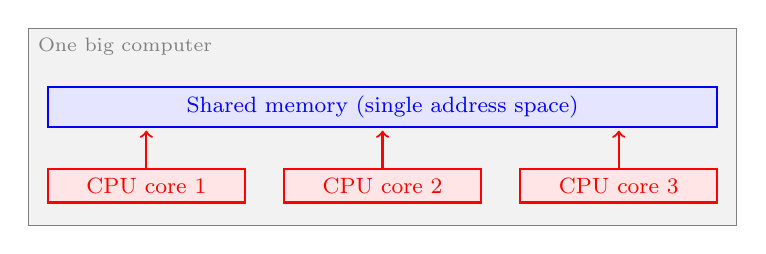
\begin{tikzpicture}
            \tikzstyle{cpu}=[draw=red, fill=red!10, thick, minimum width=2.5cm, font=\footnotesize]
            \tikzstyle{memory}=[blue, draw=blue, fill=blue!10, thick, minimum width=8.5cm, font=\footnotesize]
            \draw [black!50, fill=black!5] (0, 0) rectangle (9, 2.5);
            \node [black!50, anchor=north west, font=\scriptsize] at (0, 2.5) {One big computer};
            \node [memory] at (4.5, 1.5) {Shared memory (single address space)};
            \draw [thick, red, ->] (1.5, 0.5) node [cpu] {CPU core 1} -- (1.5, 1.2);
            \draw [thick, red, ->] (4.5, 0.5) node [cpu] {CPU core 2} -- (4.5, 1.2);
            \draw [thick, red, ->] (7.5, 0.5) node [cpu] {CPU core 3} -- (7.5, 1.2);
        \end{tikzpicture}
    \end{center}

    Message-passing distributed systems:
    \begin{center}
        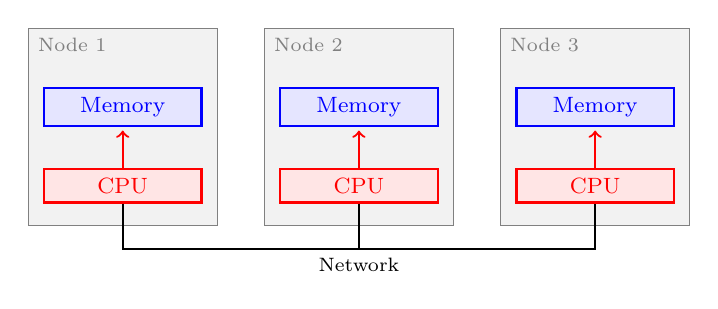
\begin{tikzpicture}
            \tikzstyle{machine}=[black!50, anchor=north west, font=\scriptsize]
            \tikzstyle{cpu}=[draw=red, fill=red!10, font=\footnotesize, thick, minimum width=2cm]
            \tikzstyle{memory}=[blue, draw=blue, fill=blue!10, font=\footnotesize, thick, minimum width=2cm]
            \draw [machine, fill=black!5] (0.3, 0) rectangle (2.7, 2.5);
            \draw [machine, fill=black!5] (3.3, 0) rectangle (5.7, 2.5);
            \draw [machine, fill=black!5] (6.3, 0) rectangle (8.7, 2.5);
            \node [machine] at (0.3, 2.5) {Node 1};
            \node [machine] at (3.3, 2.5) {Node 2};
            \node [machine] at (6.3, 2.5) {Node 3};
            \node [memory] at (1.5, 1.5) {Memory};
            \node [memory] at (4.5, 1.5) {Memory};
            \node [memory] at (7.5, 1.5) {Memory};
            \draw [thick, red, ->] (1.5, 0.5) node [cpu] (t1) {CPU} -- (1.5, 1.2);
            \draw [thick, red, ->] (4.5, 0.5) node [cpu] (t2) {CPU} -- (4.5, 1.2);
            \draw [thick, red, ->] (7.5, 0.5) node [cpu] (t3) {CPU} -- (7.5, 1.2);
            \draw [thick] (t1.south) -- (1.5, -0.3) -- (7.5, -0.3) -- (t3.south);
            \draw [thick] (t2.south) -- (4.5, -0.3);
            \node [anchor=north, font=\scriptsize] at (4.5, -0.3) {Network};
        \end{tikzpicture}
    \end{center}
\end{frame}
\inlineslide{s:shared-memory}{}

(Message-passing is sometimes also used among threads on the same machine.
Conversely, limited forms of distributed shared memory exist in some supercomputers and research systems, and there are technologies like \emph{remote direct memory access} (RDMA) that allow computers to access each others' memory over a network.
Also, databases can in some sense be regarded as shared memory, but with a different data model compared to byte-addressable memory.
However, most practical distributed systems are based on message-passing.)

\begin{frame}
    \label{s:dist-sys-definition}
    \frametitle{A distributed system is\dots}
    \begin{itemize}
        \item Multiple ``nodes'' (computers, servers, phones, \dots)
        \item communicating via an unreliable network
        \item trying to achieve some task together
    \end{itemize}\vspace{1em}\pause
    \rowcolors[]{2}{}{blue!10}
    \renewcommand{\arraystretch}{1.3}
    \begin{tabular}{p{5cm}|p{5cm}}
        \hline
        \textbf{shared memory} & \textbf{distributed system} \\\hline
        hardware fails \newline$\Rightarrow$ all threads stop & one machine fails \newline$\Rightarrow$ others continue running \pause\\
        reliable communication\newline between CPU cores & unreliable network \pause\\
        locks, semaphores, atomic\newline instructions (e.g.\ CAS) & only message-passing \\\hline
    \end{tabular}
\end{frame}
\inlineslide{s:dist-sys-definition}{}

Each of the computers in a distributed system is called a \emph{node}.
Here, ``computer'' is interpreted quite broadly: nodes might be desktop computers, servers in datacenters, mobile devices, internet-connected cars, industrial control systems, sensors, or many other types of device.
In this course we don't distinguish them: a node can be any type of communicating computing device.

In a single computer, if one component fails (e.g.\ one of the RAM modules develops a fault), we normally don't expect the computer to continue working nevertheless: it will probably just crash.
Software does not need to be written in a way that explicitly deals with faulty RAM.
However, in a distributed system we often \emph{do} want to tolerate some parts of the system being broken, and for the rest to continue working.
For example, if one node has crashed (a \emph{partial failure}), the remaining nodes may still be able to continue providing the service.

\subsection{About distributed systems}\label{sec:about}

These notes and lectures should be self-contained, but if you would like to read up on further detail, there are several suggested textbooks:
\begin{itemize}
    \item Maarten van Steen and Andrew S.\ Tanenbaum. \emph{Distributed Systems}. ISBN 978-1543057386.
        Free download from \url{https://www.distributed-systems.net/index.php/books/ds3/} (third edition, 2017).

        This book gives a broad overview over a large range of distributed systems topics, with lots of examples from practical systems.

    \item Christian Cachin, Rachid Guerraoui, and Luís Rodrigues.
        \emph{Introduction to Reliable and Secure Distributed Programming}.
        Second edition, Springer, 2011. ISBN 978-3-642-15259-7.

        Ebook download for Cambridge users: \url{https://link.springer.com/book/10.1007/978-3-642-15260-3} then click Log in $\rightarrow$ via your Institution $\rightarrow$ type \emph{University of Cambridge} $\rightarrow$ log in with Raven.

        This book is more advanced, going into depth on several important distributed algorithms, and proving their correctness.
        Recommended if you want to explore the theory in greater depth than this course covers.

    \item Martin Kleppmann. \emph{Designing Data-Intensive Applications}, O'Reilly, 2017. ISBN 978-1449373320.

        This book goes more in the direction of databases, but also covers a number of distributed systems topics.
        It is designed for software engineers in industry working with distributed databases.

    \item Jean Bacon and Tim Harris. \emph{Operating Systems: Concurrent and Distributed Software Design}.
        Addison-Wesley, 2003. ISBN 978-0321117892.

        This book provides a link to the \emph{concurrent systems} half of the course, and to operating systems topics.
        It is now sadly out of print, but you can find copies in many college libraries.
\end{itemize}

Where appropriate, these lecture notes also contain references to research papers and other useful background reading (these are given in square brackets, and the details appear at the end of this document).
However, only material covered in the lectures and these notes is examinable.

\begin{frame}
    \label{s:reading}
    \frametitle{Recommended reading}
    \begin{itemize}
        \item van Steen \& Tanenbaum.\\ ``\textbf{Distributed Systems}''\\(any ed), free ebook available
        \item Cachin, Guerraoui \& Rodrigues. \\ ``\textbf{Introduction to Reliable and Secure Distributed Programming}'' (2nd ed), Springer 2011
        \item Kleppmann.\\ ``\textbf{Designing Data-Intensive Applications}'',\\O’Reilly 2017
        \item Bacon \& Harris.\\ ``\textbf{Operating Systems: Concurrent and Distributed Software Design}'', Addison-Wesley 2003
    \end{itemize}
\end{frame}
\inlineslide{s:reading}{}

As for other courses, past exam questions are available at \url{https://www.cl.cam.ac.uk/teaching/exams/pastpapers/t-ConcurrentandDistributedSystems.html}.
The syllabus, slides, and lecture notes for this course were substantially updated and revised in 2020/21.
Because of syllabus changes, the following past exam questions are no longer applicable: 2018~P5~Q8; 2015~P5~Q8; 2014~P5~Q9~(a); 2013~P5~Q9; 2011~P5~Q8~(b).

These notes also contain exercises, which are suggested material for discussion in supervisions.
Solution notes for supervisors are available from the course web page.

This course is related to several other courses in the tripos, as shown on \autoref{l:other-courses}.

\begin{frame}
    \label{s:other-courses}
    \frametitle{Relationships with other courses}
    \begin{itemize}
        \item \textbf{Concurrent Systems} -- Part IB\\
            (every distributed system is also concurrent)
        \item \textbf{Operating Systems} -- Part IA\\
            (inter-process communication, scheduling)
        \item \textbf{Databases} -- Part IA\\
            (many modern databases are distributed)
        \item \textbf{Computer Networking} -- \whenisnetworking\\
            (distributed systems involve network communication)
        \item \textbf{Further Java} -- Part IB Michaelmas\\
            (distributed programming practical exercises)
        \item \textbf{Cybersecurity} -- \whenissecurity\\
            (web and internet security)
        \item \textbf{Cloud Computing} -- Part II\\
            (distributed systems for processing large amounts of data)
    \end{itemize}
\end{frame}
\inlineslide{s:other-courses}{}\label{l:other-courses}

There are a number of reasons for creating distributed systems.
Some applications are \emph{intrinsically distributed}: if you want to send a message from your phone to your friend's phone, that operation inevitably requires those phones to communicate via some kind of network.

Some distributed systems do things that in principle a single computer could do, but they do it \emph{more reliably}.
A single computer can fail and might need to be rebooted from time to time, but if you are using multiple nodes, then one node can continue serving users while another node is rebooting.
Thus, a distributed system has the potential to be more reliable than a single computer, at least if it is well-designed!

Another reason for distribution is for better \emph{performance}: if a service has users all over the world, and they all have to access a single node, then either the users in the UK or the users in New Zealand are going to find it slow (or both).
By placing nodes in multiple locations around the world, we can get around the slowness of the speed of light by routing each user to a nearby node.

Finally, some large-scale data processing or computing tasks are simply \emph{too big} to perform on a single computer, or would be intolerably slow.
For example, the Large Hadron Collider at CERN is supported by a worldwide computing infrastructure with 1 million CPU cores for data analysis, and 2 exabytes ($2 \cdot 10^{18}$ bytes) of storage! See \url{https://wlcg-public.web.cern.ch/}.

\begin{frame}
    \label{s:why-distribute}
    \frametitle{Why make a system distributed?}
    \begin{itemize}\pause
        \item \textbf{It's inherently distributed:}\\e.g. sending a message from your mobile phone to your friend's phone\pause
        \item \textbf{For better reliability:}\\even if one node fails, the system as a whole keeps functioning\pause
        \item \textbf{For better performance:}\\get data from a nearby node rather than one halfway round the world\pause
        \item \textbf{To solve bigger problems:}\\e.g. huge amounts of data, can't fit on one machine
    \end{itemize}
\end{frame}
\inlineslide{s:why-distribute}{}\label{l:why-distribute}

However, there are also downsides to distributed systems, because things can go wrong, and the system needs to deal with such faults.
The network may fail, leaving the nodes unable to communicate.

\begin{frame}
    \label{s:no-internet}
    
\includegraphics[height=\paperheight]{images/no-internet.png}
\end{frame}
\inlineslide{s:no-internet}{}

Another thing that can go wrong is that a node may crash, or run much slower than usual, or misbehave in some other way (perhaps due to a software bug or a hardware failure).
If we want one node to take over when another node crashes, we need to detect that a crash has happened; as we shall see, even that is not straightforward.
Network failures and node failures can happen at any moment, without warning.

If one component of a system stops working, we call that a \emph{fault}, and many distributed systems strive to provide \emph{fault tolerance}: that is, the system as a whole continues functioning despite the fault.
Dealing with faults is what makes distributed computing fundamentally different, and often harder, compared to programming a single computer.
Some distributed system engineers believe that if you can solve a problem on a single computer, it is basically easy!
Though, in fairness to our colleagues in other areas of computer science, this is probably not true.

\begin{frame}
    \label{s:why-not}
    \frametitle{Why NOT make a system distributed?}
    The trouble with distributed systems:
    \begin{itemize}
        \item Communication may fail (and we might not even know it has failed).
        \item Processes may crash (and we might not know).
        \item All of this may happen nondeterministically and without warning.
    \end{itemize}\vspace{1em}\pause
    \textbf{Fault tolerance}: we want the system as a whole to continue working, even when some parts are faulty.\\[1em]
    This is hard.\\[1em]
    Writing a program to run on a single computer is comparatively easy?!
\end{frame}
\inlineslide{s:why-not}{}

A practical goal in many distributed systems is to ensure the system provides consistently good performance and availability, especially as the system grows to handle larger volumes of requests and data (\emph{scalability}).
On the other hand, the theory of distributed systems focuses primarily on ensuring that certain correctness guarantees are always met.
This difference in emphasis leads us to pay attention to different things: to achieve good performance, what matters is to optimise the operations that happen frequently; to achieve correctness, we have to also examine the obscure edge cases that occur infrequently (but which cannot be ruled out entirely).

\begin{frame}
    \label{s:theory-practice}
    \frametitle{Theory and practice}
    \textbf{Practice:}\\ How can we achieve good performance in the common case? \\[1em]
    \textbf{Theory:}\\ How can we guarantee correctness in all possible scenarios? \pause\\[1em]
    Build a system without understanding the theory?
    \begin{itemize}
        \item works fine for a while\dots\\
        \item but one day it fails catastrophically due to some weird edge case, and corrupts all your data
            \raisebox{-2pt}{
\includegraphics[height=12pt]{images/1f62d.pdf}} \pause\\[1em]
    \end{itemize}
    \raisebox{-2pt}{
\includegraphics[height=12pt]{images/26a0.pdf}} 
    Distributed systems are notoriously hard to get right.\\
    The theory helps us build robust systems.
\end{frame}
\inlineslide{s:theory-practice}{}\label{l:theory-practice}

Many practical systems have suffered severe bugs, often causing data loss, because their designers did not understand the theoretical foundations.
Distributed systems are notoriously subtle and difficult to get right, and theory is the best tool we have for making sense of this complexity.
Having a good grasp of distributed systems theory is very valuable for making practical systems reliable and preventing catastrophic bugs.
This course therefore places greater emphasis on the theory than on the practical techniques for achieving high performance.

\subsection{Distributed systems and computer networking}\label{sec:networking}

The web is an example of a distributed system that you use every day.

\begin{frame}[plain]
    \label{s:website}
    \begin{tikzpicture}[remember picture,overlay]
        \node at (current page.center) {
\includegraphics[height=\paperheight]{images/website.png}};
    \end{tikzpicture}
\end{frame}
\inlineslide{s:website}{}

The computers that make up the web play two main roles: \emph{servers} host websites, and \emph{clients} (web browsers) display them.
When you load a web page, your web browser sends a \emph{HTTP request} message to the appropriate server.
On receiving that request, the web server sends a \emph{response} message containing the page contents to the client that requested it.
These messages are normally invisible, but we can capture and visualise the network traffic with a tool such as Charles (\url{https://www.charlesproxy.com/}), shown on \autoref{l:http-capture}.

\begin{frame}
    \label{s:client-server}
    \frametitle{Client-server example: the web}
    Time flows from top to bottom.
    \begin{center}
        \begin{tikzpicture}
            \node [rectangle,fill=red!10,draw] (client) at (0,4) {client};
            \node [rectangle,fill=red!10,draw] (server) at (8,4) {server www.cst.cam.ac.uk};
            \draw (client) -- (0,0);
            \draw (server) -- (8,0);
            \draw<2-> [bigarrow] (0,3) -- node [above,sloped] {GET \coursepath} (8,2);
            \draw<3> [bigarrow] (8,1.5) -- node [above,sloped] {\texttt{<!DOCTYPE html><html>...}} (0,0.5);
        \end{tikzpicture}
    \end{center}
\end{frame}
\inlineslide{s:client-server}{}

In a URL such as \courseurl, the part between the \verb|//| and the following \verb|/| is the hostname of the server to which the client is going to send the request (\texttt{www.cst.cam.ac.uk}), and the rest (\texttt{\coursepath}) is the path that the client asks for in its request message.
Besides the path, the request also contains some extra information, such as the HTTP method (e.g.\ \texttt{GET} to load a page, or \texttt{POST} to submit a form), the version of the client software (the \emph{user-agent}), and a list of file formats that the client understands (the \emph{accept header}).
The response message contains the file that was requested, and an indicator of its file format (the \emph{content-type}); in the case of a web page, this might be a HTML document, an image, a video, a PDF document, or any other type of file.

\begin{frame}[plain]
    \label{s:http-capture}
    \begin{tikzpicture}
        \node at (0,0) {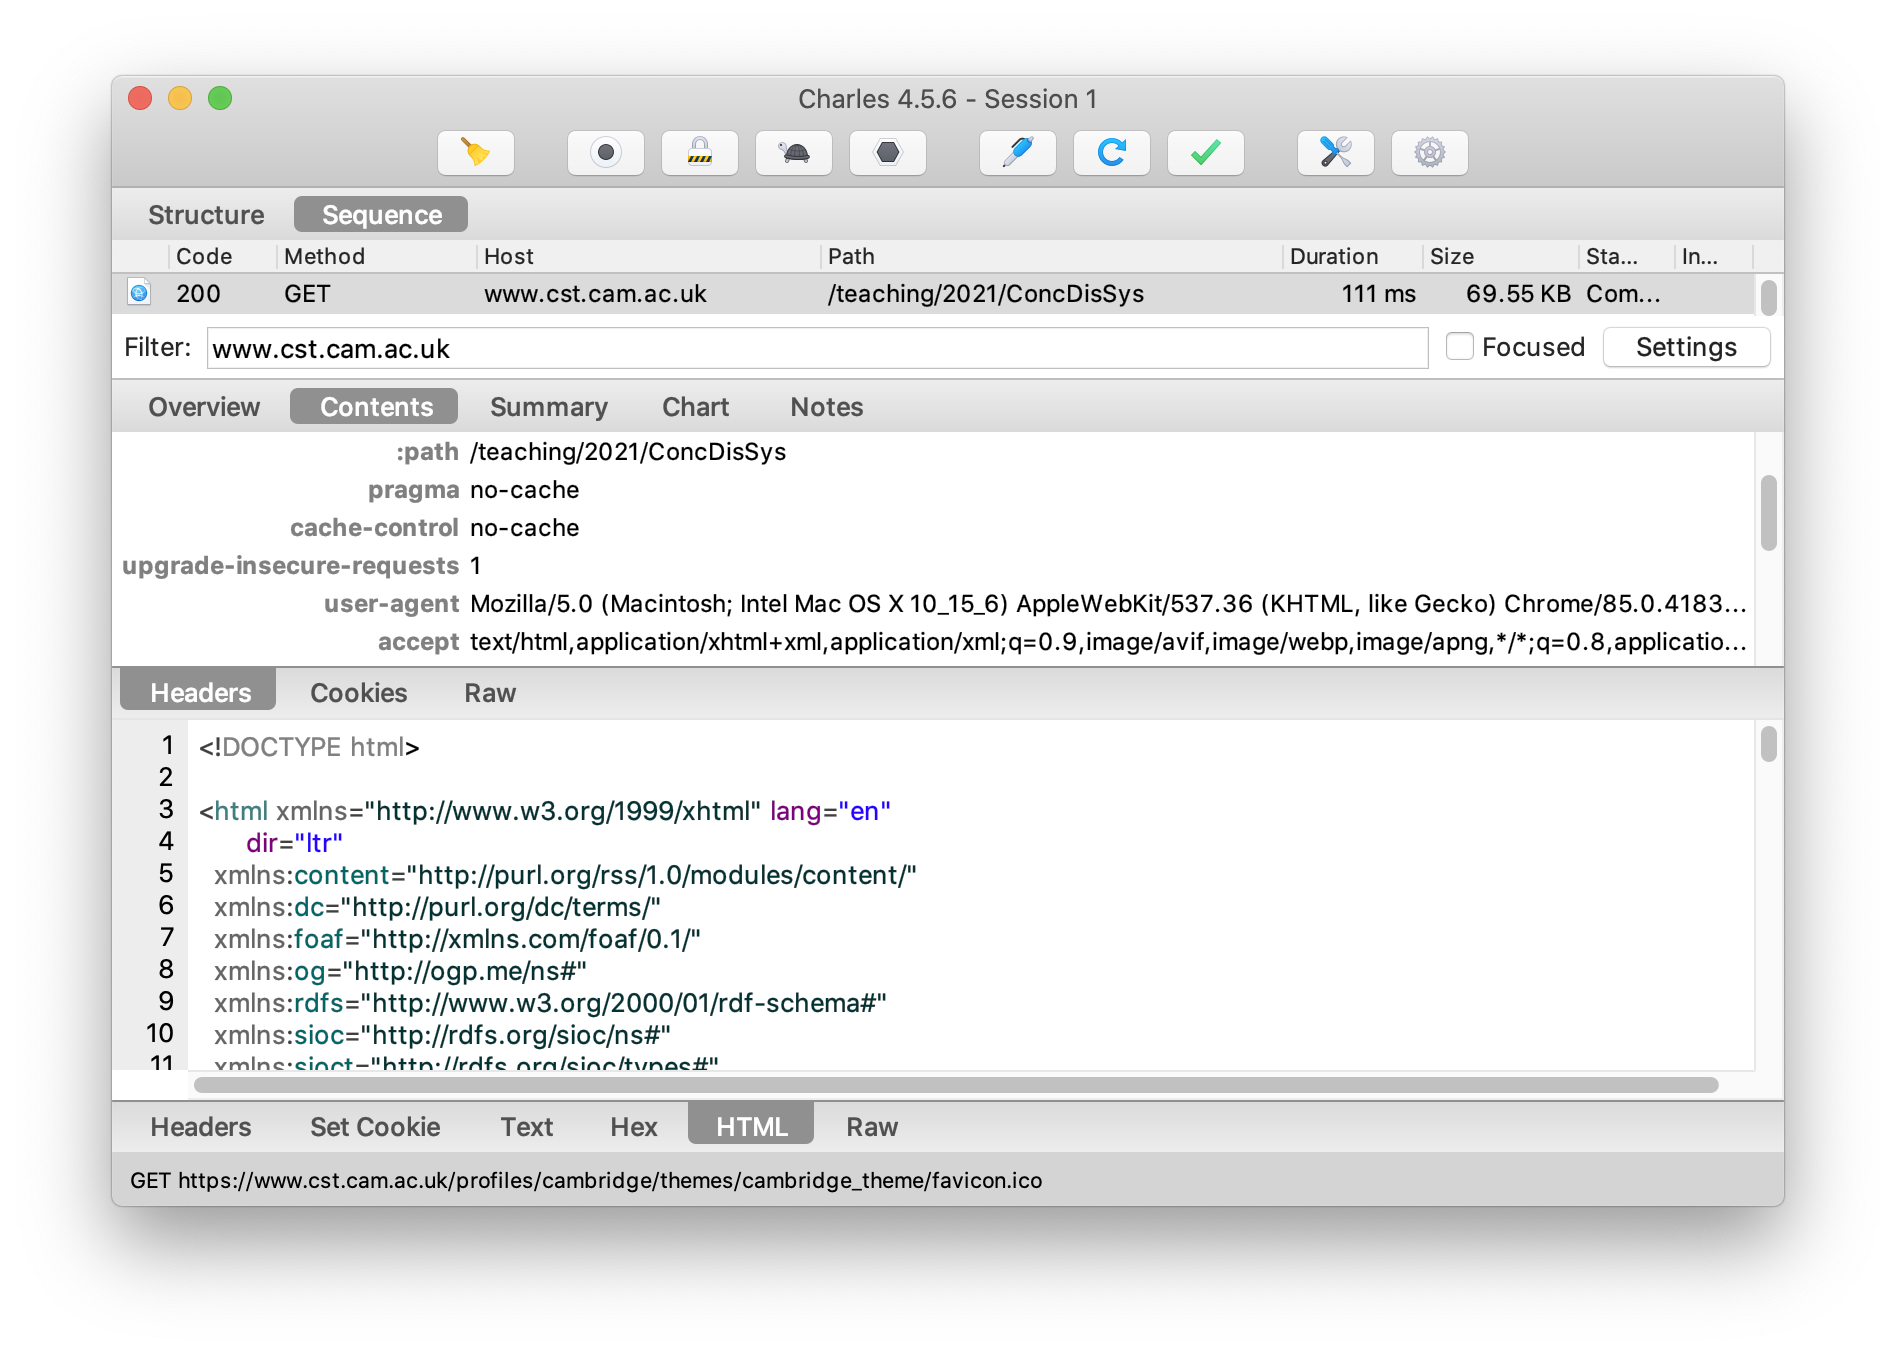
\includegraphics[height=8cm]{images/http-capture.png}};
        \node<2> (request) at (-4,-4.5) [red] {request message};
        \node<2> (response) at (2,-4.5) [red] {response message};
        \draw<2> [-Stealth,red,line width=4pt] (request) -- (-4,1.0);
        \draw<2> [-Stealth,red,line width=4pt] (response) -- (0,-1.2);
    \end{tikzpicture}
\end{frame}
\inlineslide{s:http-capture}{}\label{l:http-capture}

Since the requests and responses can be larger than we can fit in a single network packet, the HTTP protocol runs on top of TCP, which breaks down a large chunk of data into a stream of small network packets (see \autoref{l:wireshark}), and puts them back together again at the recipient.
(TCP will be discussed in detail in the \href{\networking}{Computer Networking} course.)
HTTP also allows multiple requests and multiple responses to be sent over a single TCP connection.

\begin{frame}[plain]
    \label{s:wireshark}
    \begin{tikzpicture}[remember picture,overlay]
        \node at (current page.center) {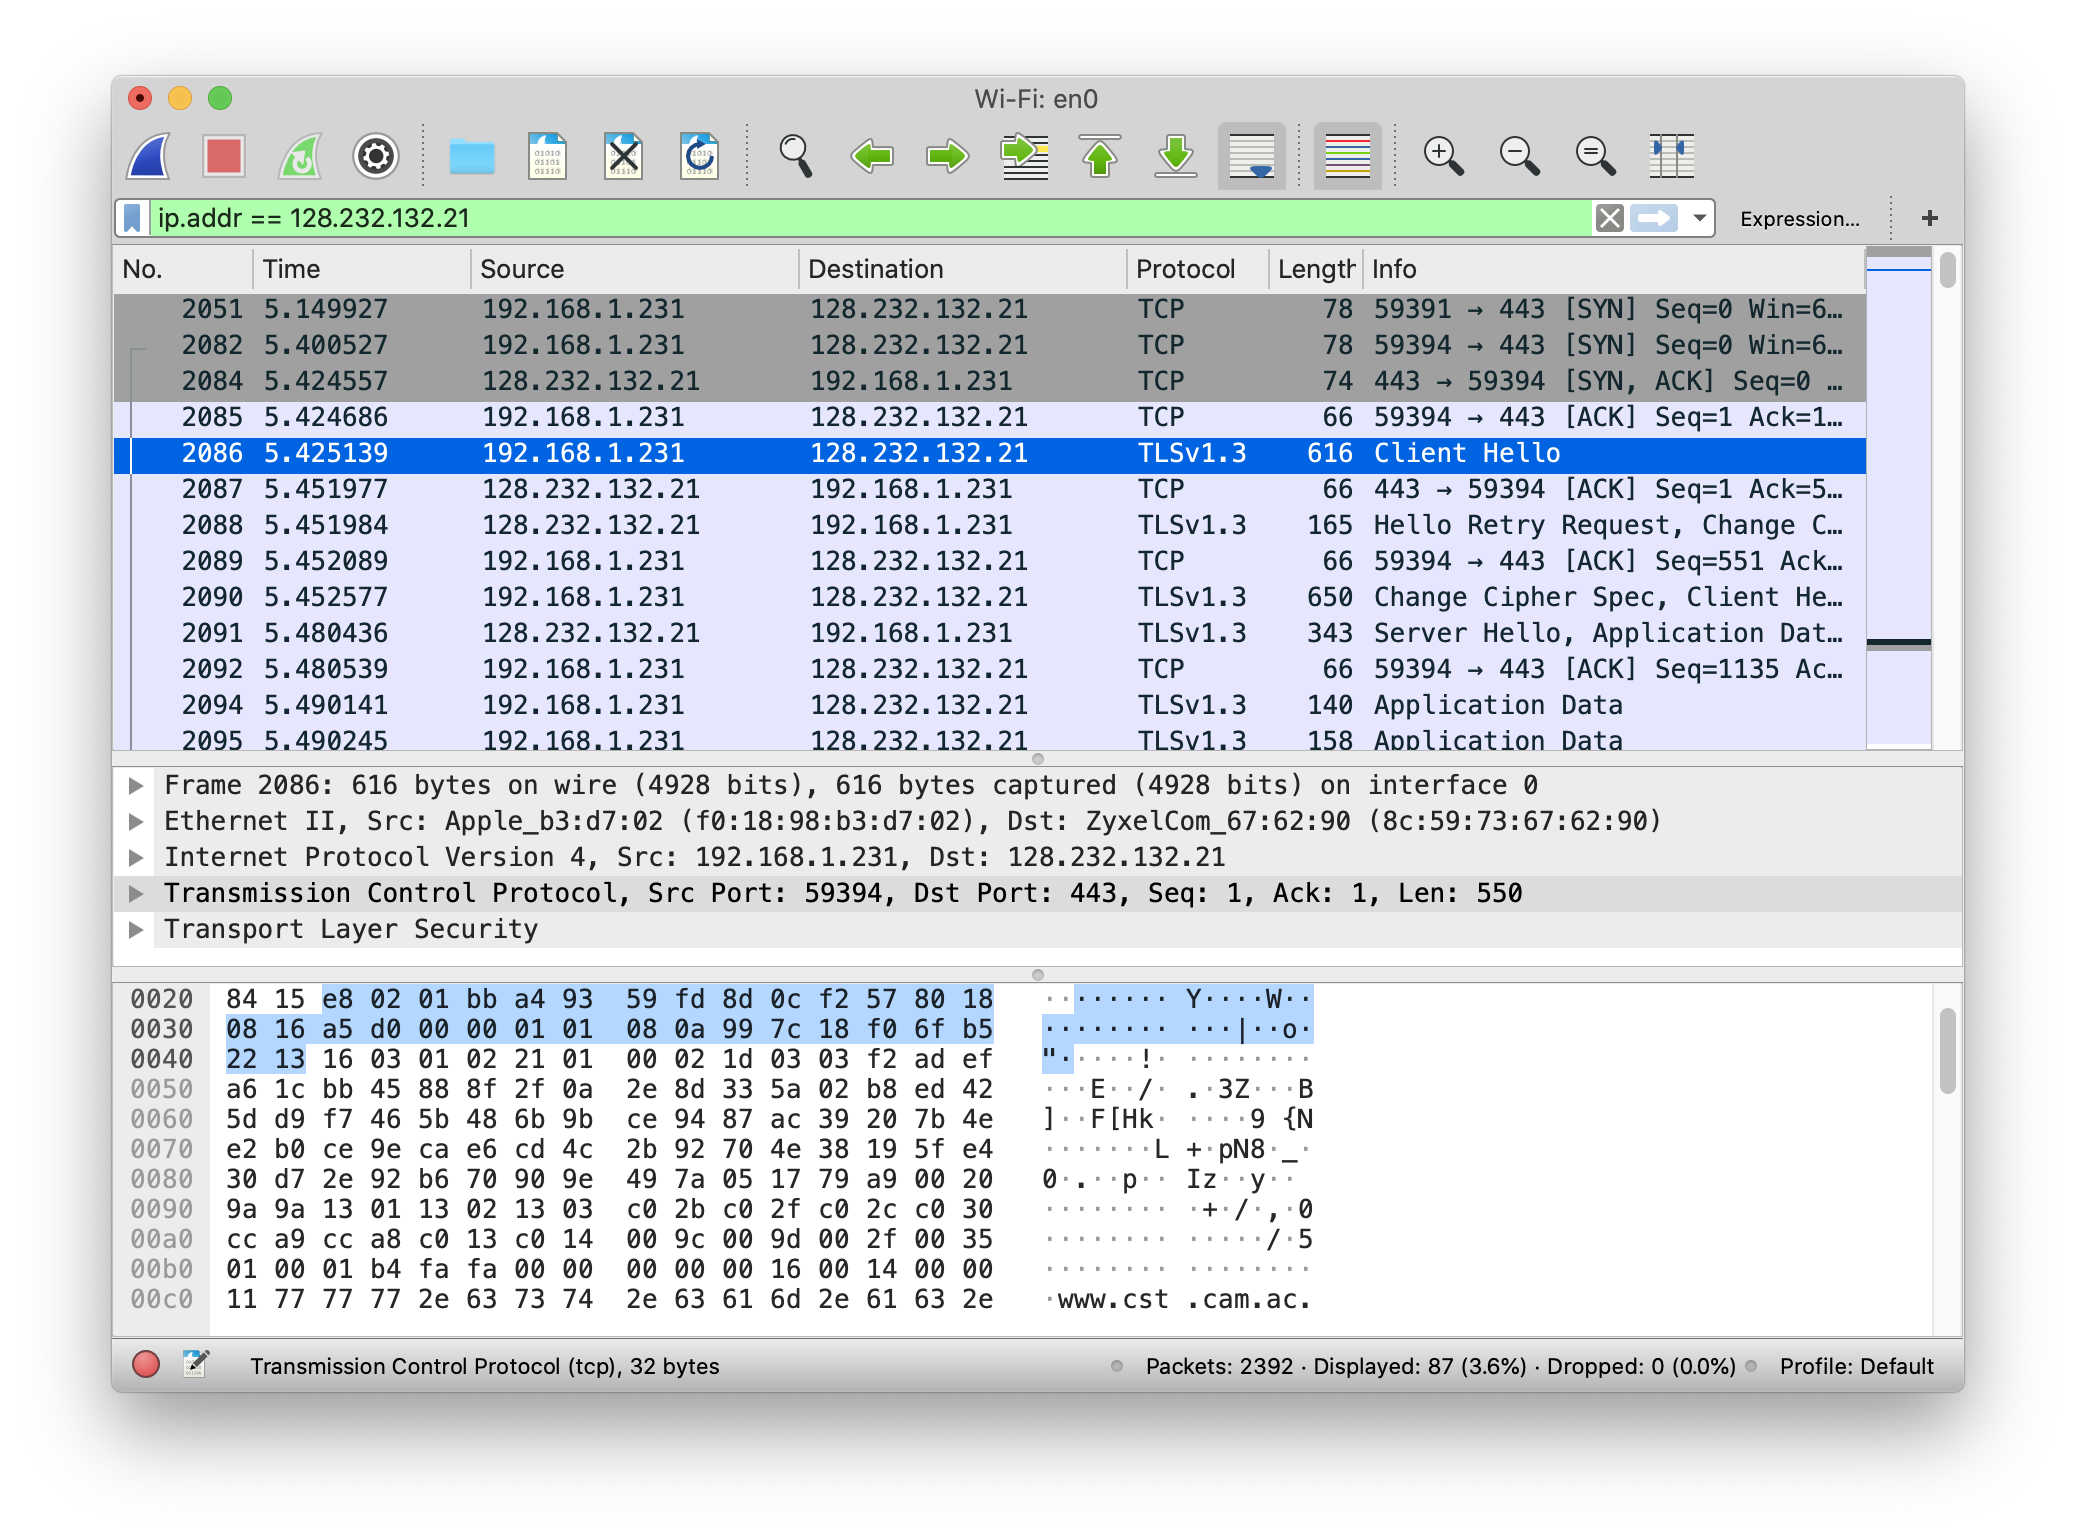
\includegraphics[height=\paperheight]{images/wireshark.png}};
    \end{tikzpicture}
\end{frame}
\inlineslide{s:wireshark}{}\label{l:wireshark}

\supervision{
    A TCP connection allows two nodes to send each other arbitrarily long sequences of bytes.
    You decide that you want to send multiple requests and responses over the same TCP connection.
    What do you need to do in order to implement such a request-response protocol using TCP?
}{
    Once you have encoded a request or response message as a sequence of bytes, you need some way for the sender of a message to tell the recipient where one request/response ends and the next one begins.
    This is known as \emph{message framing}.
    One way is for each message to contain a header indicating the size of the following message in bytes.
    Another approach is to reserve a certain sequence of bytes as message separator, and ensure that this sequence cannot occur in the middle of a message (for example, HTTP/1.1 uses \texttt{{\char`\\}r{\char`\\}n{\char`\\}r{\char`\\}n} as message separator for requests).

    Next, to associate requests and responses, one option is to rely on ordering: the first response sent by one node corresponds to the first request sent by the other node, and so on for the second, third, etc.\ request/response (HTTP/1.1 uses this approach).
    A downside of this approach is that if one request is slow to process, all of the following requests must wait until the slow one is complete before their responses can be sent (this is known as \emph{head-of-line blocking}).
    An alternative is to give each request a unique ID of some sort, and for each response to quote the ID of the request it is responding to.
    That allows the responses to be sent in a different order from the requests, which means a response can be sent as soon as it is ready, without waiting for other requests (HTTP/2 works like this).
}

However, when looking at this protocol from a distributed systems point of view, this detail is not important: we treat the request as one message and the response as another message, regardless of the number of physical network packets involved in transmitting them.
This keeps things independent of the underlying networking technology.

In the following lectures, we just assume that there is some way for one node to send a message to another node.
We don't particularly care how messages are physically represented or encoded~-- the network protocols, informally known as the \emph{bytes on the wire}~-- because the basic principle of sending and receiving messages remains the same, even as particular networking technologies come and go.
The ``wire'' may actually be radio waves, lasers, a USB thumb drive in someone's pocket, or even hard drives in a van.

\begin{frame}
    \label{s:networking}
    \frametitle{Abstracting over networking details}
    Network packets are too much low-level detail.

    We use a simple abstraction of communication:
    \begin{center}
        \begin{tikzpicture}
            \node [circle,fill=red!10,draw] (i) at (0,0) {node $i$};
            \node [circle,fill=red!10,draw] (j) at (6,0) {node $j$};
            \draw [bigarrow] (i) -- node [above] {message $m$} (j);
        \end{tikzpicture}
    \end{center}\pause

    Reality is much more complex:
    \begin{itemize}
        \item \textbf{Node:}\\ server, desktop computer, phone, car, robot, sensor, \dots\pause
        \item \textbf{Various network operators:}\\ eduroam, home DSL, cellular data, coffee shop wifi, submarine cable, satellite\dots\pause
        \item \textbf{Physical communication:}\\ electric current, radio waves, laser, hard drives in a van\dots
    \end{itemize}
\end{frame}
\inlineslide{s:networking}{}

\begin{frame}[plain]
    \label{s:snowball}
    \frametitle{Hard drives in a van?!}
    \begin{center}
        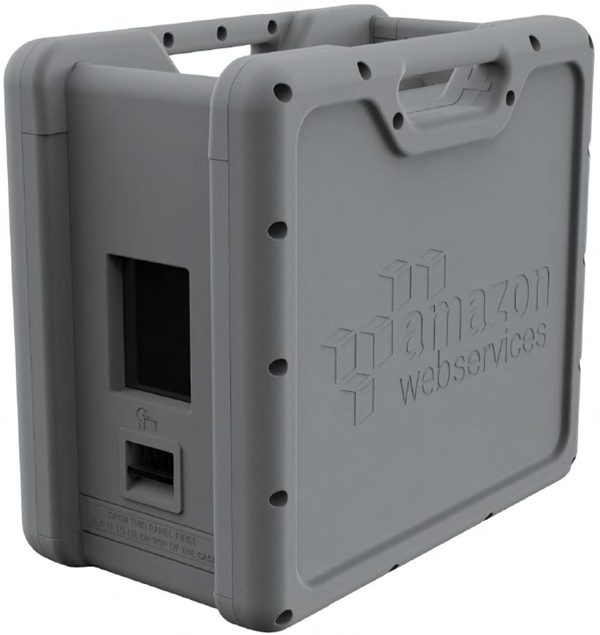
\includegraphics[height=5cm]{images/aws-snowball.png}\\[0.5em]
        {\scriptsize\url{https://docs.aws.amazon.com/snowball/latest/ug/using-device.html}}\\[1em]
        High latency, high bandwidth!
    \end{center}
\end{frame}
\inlineslide{s:snowball}{}

% Snowmobile is a whole shipping container full of hard drives https://aws.amazon.com/snowmobile/

Indeed, if you want to send a very large message (think tens of terabytes), it would be slow to send that data over the Internet, and it is in fact faster to write that data to a bunch of hard drives, load them into a van, and to drive them to their destination.
But from a distributed systems point of view, the method of delivering the message is not important: we only see an abstract communication channel with a certain \emph{latency} (delay from the time a message is sent until it is received) and \emph{bandwidth} (the volume of data that can be transferred per unit time).

\begin{frame}
    \label{s:latency-bandwidth}
    \frametitle{Latency and bandwidth}
    \textbf{Latency}: time until message arrives
    \begin{itemize}
        \item In the same datacenter: $\approx 100$ {\textmu}s
        \item One continent to another: $\approx 100$ ms
        \item Hard drives in a van: $\approx 1$ day\\[2em]
    \end{itemize}\pause
    \textbf{Bandwidth}: data volume per unit time
    \begin{itemize}
        \item 4G cellular data: $\approx 10$ Mbit/s
        \item Home broadband: $\approx 100$ Mbit/s
        \item Hard drives in a van: 50~TB/box $\approx 1$ Gbit/s
        \item In the same datacenter: $\approx 10$ Gbit/s\\[1em]
    \end{itemize}
    (Very rough numbers, vary hugely in practice!)
\end{frame}
\inlineslide{s:latency-bandwidth}{}
% Datacenter network stats: https://github.com/sirupsen/napkin-math

The \href{\networking}{Computer Networking} course (\whenisnetworking) focusses on the network protocols that enable messages to get to their destination.
Distributed systems build upon that facility, and instead focus on how several nodes should coordinate in order to achieve some shared task.
The design of distributed algorithms is about deciding what messages to send, and how to process the messages when they are received.

There are also differences in perspective.
For example, TCP is often described as providing a ``reliable'' way of transferring data over a network, in the sense that if packets are lost in transit, the TCP implementation will automatically retransmit the lost packets and put them back in the correct order at the recipient.
However, if too many packets are lost, TCP gives up and returns a timeout error.
Depending on the network, such extended packet loss might be a rare occurrence, but it can certainly happen~-- for example, if someone unplugs the network cable.
From a theoretical point of view, it is therefore not correct to call TCP ``reliable'', since there is a nonzero risk that it fails to correctly deliver a message.

\begin{frame}
    \label{s:networking2}
    \frametitle{Distributed Systems and Networking}
    \rowcolors[]{2}{}{blue!10}
    \renewcommand{\arraystretch}{1.3}
    \begin{tabular}{p{5cm}|p{5cm}}
        \hline
        \textbf{networking} & \textbf{distributed systems} \\\hline
        how to get data from A to B \newline (packets, routing, \dots) & how to achieve some goal by sending/receiving messages \pause\\
        ``TCP is reliable'' \newline (dropped packets are automatically retransmitted) & any message can be lost \newline (unplug the network cable \newline$\Rightarrow$ TCP timeout) \\\hline
    \end{tabular}
    \begin{center}
        % Source for network-cable.jpg: https://pixabay.com/photos/modem-antenna-wire-cable-router-5436144/
        % (Royalty-free, no attribution required)
        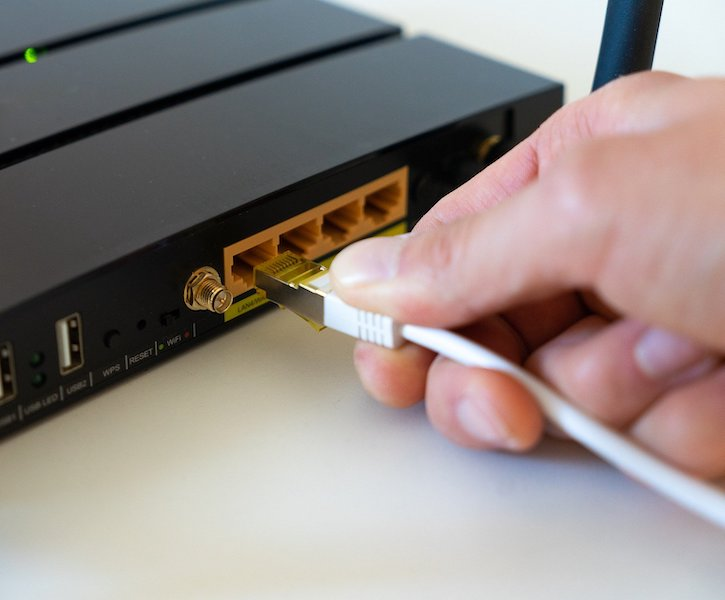
\includegraphics[width=4cm]{images/network-cable.jpg}
    \end{center}
\end{frame}
\inlineslide{s:networking2}{}\label{l:networking2}

\subsection{Availability and fault tolerance}\label{sec:availability}

\begin{frame}
    \label{s:availability}
    \frametitle{Availability}
    Online shop wants to sell stuff 24/7! \\
    Service unavailability = downtime = losing money \\[1em]
    Availability = uptime = fraction of time that a service is functioning correctly
    \begin{itemize}
        \item ``Two nines'' = 99\% up = down 3.7 days/year
        \item ``Three nines'' = 99.9\% up = down 8.8 hours/year
        \item ``Four nines'' = 99.99\% up = down 53 minutes/year
        \item ``Five nines'' = 99.999\% up = down 5.3 minutes/year\\[1.5em]
    \end{itemize}\pause
    \textbf{Service-Level Objective} (SLO):\\ e.g. ``99.9\% of requests in a day get a response in 200~ms''\\[1em]
    \textbf{Service-Level Agreement} (SLA):\\ contract specifying some SLO, penalties for violation
\end{frame}
\inlineslide{s:availability}{}\label{l:availability}

From a business point of view, what usually matters most is the \emph{availability} of a service, such as a website.
For example, an online shop wants to be able to sell products at any time of day or night: any outage of the website means a lost opportunity to make money.
For other services, there may even be contractual agreements with customers requiring the service to be available.
If a service is unavailable, this can also damage the reputation of the service provider.

The availability of a service is typically measured in terms of its ability to respond correctly to requests within a certain time.
The definition of whether a service is ``available'' or ``unavailable'' can be somewhat arbitrary: for example, if it takes 5 seconds to load a page, do we still consider that website to be available?
What if it takes 30 seconds?
An hour?

Typically, the availability expectations of a service are formalised as a \emph{service-level objective} (SLO), which typically specifies the percentage of requests that need to return a correct response within a specified timeout, as measured by a certain client over a certain period of time.
A \emph{service-level agreement} (SLA) is a contract that specifies some SLO, as well as the consequences if the SLO is not met (for example, the service provider may need to offer a refund to its customers).

Faults (such as node crashes or network interruptions) are a common cause of unavailability.
In order to increase availability, we can reduce the frequency of faults, or we can design systems to continue working despite some of its components being faulty; the latter approach is called \emph{fault tolerance}.
Reducing the frequency of faults is possible through buying higher-quality hardware and introducing redundancy, but this approach can never reduce the probability of faults to zero.
Instead, fault tolerance is the approach taken by many distributed systems.

Tolerating faults also makes day-to-day operations easier: for example, if a service can tolerate one out of three nodes being unavailable, then a software upgrade can be rolled out by installing it and restarting one node at a time, while the remaining two nodes continue providing the service.
Being able to roll out software upgrades in this way, without clients noticing any interruption, is important for many organisations that are continually working to improve their software, because it allows the software to be updated frequently.

\begin{frame}
    \label{s:fault-tolerance}
    \frametitle{Achieving high availability: fault tolerance}
    \textbf{Failure}: system as a whole isn't working\\
    \textbf{Fault}: some part of the system isn't working
    \begin{itemize}
        \item Node fault: crash, deadlock, \dots
        \item Network fault: dropping or significantly delaying messages\pause\\[1em]
    \end{itemize}
    To increase availability: have fewer faults, or \textbf{tolerate} faults\\[1em]
    \textbf{Fault tolerance}:\\system as a whole continues working, despite faults\\
    (up to some maximum number of faults)\pause\\[1em]
    \textbf{Single point of failure} (SPOF):\\ node/network link whose fault leads to failure\\[1em]
    Fault tolerance is also useful for \textbf{software updates}:\\ reboot one node at a time while continuing to serve users
\end{frame}
\inlineslide{s:fault-tolerance}{}\label{l:fault-tolerance}

Fault tolerance is always relative to the maximum number of faults that can be tolerated: for example, some distributed algorithms are able to make progress provided that fewer than half of the nodes have crashed, but they stop working if more than half the nodes crash.
It does not make sense to want to tolerate an unlimited number of faults: if all nodes crash and don't recover, then no algorithm will be able to get any work done, no matter how clever it might be.

In some systems, a single component becoming faulty would cause an outage of the entire system.
Such a component is called a \emph{single point of failure} (SPOF), and fault-tolerant generally systems try to avoid having any SPOF.
For example, the Internet is designed to have no SPOF: there is no one server or router whose destruction would bring down the entire Internet (although the loss of some components, such as key intercontinental fibre links, does cause noticeable disruption).
% Also BGP hijacking...

%\begin{frame}
    %\label{s:availability-discuss}
    %\frametitle{High availability costs and benefits}
    % TODO: visualise a rolling software upgrade?
%\end{frame}
%\inlineslide{s:availability-discuss}{}\label{l:availability-discuss}

For safety-critical applications, such as air-traffic control systems, it is undoubtedly important to invest in good fault-tolerance mechanisms.
However, it is not always the case that higher availability is better.
Reaching extremely high availability requires a highly focussed engineering effort, and often conservative design choices.
For example, the old-fashioned fixed-line telephone network is designed for ``five nines'' availability, but the downside of this focus on availability is that it has been very slow to evolve.
Most Internet services do not even reach four nines because of diminishing returns: beyond some point, the additional cost of achieving higher availability exceeds the cost of occasional downtime, so it is economically rational to accept a certain amount of downtime.

\subsection{Example: Remote Procedure Calls (RPC)}\label{sec:rpc}

Besides the web, another example of an everyday distributed system is when you buy something online using a credit/debit card.
When you enter your card number in some online shop, that shop will send a payment request over the Internet to a service that specialises in processing card payments.
The payments service in turn communicates with a card network such as Visa or MasterCard, which communicates with the bank that issued your card in order to take the payment.
For the programmers who are implementing the online shop, the code for processing the payment may look something like the code on \autoref{l:payment-rpc}.

\begin{frame}
    \label{s:payment-example}
    \frametitle{Client-server example: online payments}
    \begin{center}
        \begin{tikzpicture}
            \node [rectangle,fill=red!10,draw] (client) at (0,4) {online shop};
            \node [rectangle,fill=red!10,draw] (server) at (8,4) {payments service};
            \draw (client) -- (0,0);
            \draw (server) -- (8,0);
            \draw<2-> [bigarrow] (0,3) -- node [above,sloped] {charge {\textsterling}3.99 to credit card 1234\dots} (8,2);
            \draw<3> [bigarrow] (8,1.5) -- node [above,sloped] {success} (0,0.5);
        \end{tikzpicture}
    \end{center}
\end{frame}
\inlineslide{s:payment-example}{}

\begin{frame}
    \label{s:payment-rpc}
    \frametitle{Remote Procedure Call (RPC) example}
    \inputminted{java}{code/payment-rpc.java}
    \begin{tikzpicture}[remember picture,overlay]
        \node (call) [xshift=2cm,yshift=-0.5cm] at (current page.center) {};
        \node<2> (label) [anchor=south east,red,yshift=0.5cm] at (current page.south east) {Implementation of this function is on another node!};
        \draw<2> [-Stealth,red,line width=4pt] (label) -- (call);
    \end{tikzpicture}
\end{frame}
\inlineslide{s:payment-rpc}{}\label{l:payment-rpc}

Calling the \verb|processPayment| function looks like calling any other function, but in fact, what is happening behind the scenes is that the shop is sending a request to the payments service, waiting for a response, and then returning the response it received.
The actual implementation of \verb|processPayment|~-- the logic that communicates with the card network and the banks~-- does not exist in the code of the shop: it is part of the payments service, which is another program running on another node belonging to a different company.

This type of interaction, where code on one node appears to call a function on another node, is called a \emph{Remote Procedure Call} (RPC).
In Java, it is called \emph{Remote Method Invocation} (RMI).
The software that implements RPC is called an \emph{RPC framework} or \emph{middleware}.
(Not all middleware is based on RPC; there is also middleware that uses different communication models.)

When an application wishes to call a function on another node, the RPC framework provides a \emph{stub} in its place.
The stub has the same type signature as the real function, but instead of executing the real function, it encodes the function arguments in a message and sends that message to the remote node, asking for that function to be called.
The process of encoding the function arguments is known as \emph{marshalling}.
In the example on \autoref{l:payment-json}, a JSON encoding is used for marshalling, but various other formats are also used in practice.

\begin{frame}[plain]
    \label{s:payment-json}
    \hspace*{-1cm}
    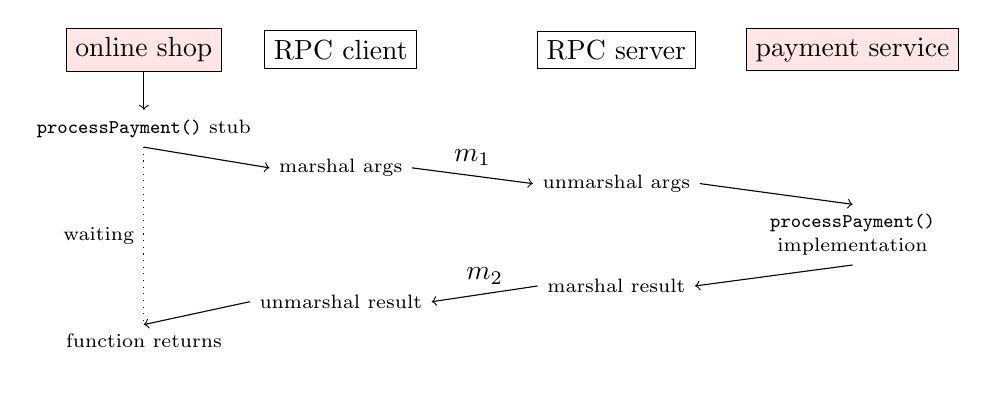
\begin{tikzpicture}
        \node [rectangle,fill=red!10,draw] (client) at (0,4) {online shop};
        \node [rectangle,draw] (rpc-client) at (2.5,4) {RPC client};
        \node [rectangle,draw] (rpc-server) at (6,4) {RPC server};
        \node [rectangle,fill=red!10,draw] (server) at (9,4) {payment service};
        \node [font=\scriptsize] (invoke) at (0,3) {\texttt{processPayment()} stub};
        \draw [->] (client) -- (invoke);
        \node<2-> [font=\scriptsize] (send-req) at (2.5,2.5) {marshal args};
        \draw<2-> [->] (invoke.south) -- (send-req.west);
        \node<2-> [font=\scriptsize] (recv-req) at (6,2.3) {unmarshal args};
        \draw<2-> [->] (send-req.east) -- node [above] {$m_1$} (recv-req.west);
        \node<3-> [font=\scriptsize] (exec) at (9,1.8) {\texttt{processPayment()}};
        \node<3-> [font=\scriptsize] (exec2) at (9,1.5) {implementation};
        \draw<3-> [->] (recv-req.east) -- (exec.north);
        \node<4-> [font=\scriptsize] (send-res) at (6,1) {marshal result};
        \draw<4-> [->] (exec2.south) -- (send-res.east);
        \node<4-> [font=\scriptsize] (recv-res) at (2.5,0.8) {unmarshal result};
        \draw<4-> [->] (send-res.west) -- node [above] {$m_2$} (recv-res.east);
        \node<5> [font=\scriptsize] (return) at (0,0.3) {function returns};
        \draw<5> [->] (recv-res.west) -- (return.north);
        \draw [dotted] (invoke.south) -- node [left,font=\scriptsize] {waiting} (0,0.5);
        \node at (0,0) {}; % so that messages below stay put as the slide builds
    \end{tikzpicture}
    \hspace*{-1cm}\mbox{
        \onslide<2->{
            $m_1$ = \begin{minipage}{5.5cm}
            \inputminted[fontsize=\scriptsize,frame=single,bgcolor=lightgrey]{json}{code/payment-rpc.json}
            \end{minipage}
        }
        \onslide<4->{
            $m_2$ = \begin{minipage}{3.8cm}
            \inputminted[fontsize=\scriptsize,frame=single,bgcolor=lightgrey]{json}{code/payment-response.json}
            \end{minipage}
        }
    }
\end{frame}
\inlineslide{s:payment-json}{}\label{l:payment-json}

The sending of the message from the RPC client to the RPC server may happen over HTTP (in which case this is also called a \emph{web service}), or one of a range of different network protocols may be used.
On the server side, the RPC framework unmarshals (decodes) the message and calls the desired function with the provided arguments.
When the function returns, the same happens in reverse: the function's return value is marshalled, sent as a message back to the client, unmarshalled by the client, and returned by the stub.
Thus, to the caller of the stub, it looks as if the function had executed locally.

\begin{frame}
    \label{s:rpc-problems}
    \frametitle{Remote Procedure Call (RPC)}
    Ideally, RPC makes a call to a remote function look the same as a local function call.\\[1em]
    \textbf{``Location transparency''}:\\ system hides where a resource is located.\\[1em]\pause
    In practice\dots
    \begin{itemize}
        \item what if the service crashes during the function call?
        \item what if a message is lost?
        \item what if a message is delayed?
        \item if something goes wrong, is it safe to retry?
    \end{itemize}
\end{frame}
\inlineslide{s:rpc-problems}{}

The difficulty with RPC is that many things can go wrong, as networks and nodes might fail.
If the client sends an RPC request but receives no response, it doesn't know whether or not the server received and processed the request.
It could resend the request if it doesn't hear back for a while, but that might cause the request to be performed more than once (e.g.\ charging a credit card twice).
Even if we retry, there is no guarantee that the retried messages will get through either.
Waiting forever is not a good approach, so in practice the client will have to give up after some timeout.

\supervision{
    How is RPC different from a local function call?
    Is location transparency achievable?
}{
    \begin{itemize}
        \item RPCs may time out if the request or response message is lost.
            Even if we retry, there is no guarantee that the messages will get through.
            The application must handle this error condition, and the possibility of failure may need to be reflected in the type signature.
            For example, Java RPC libraries often throw a checked exception, and JavaScript RPC clients often return a \emph{promise}, which can either succeed or fail.
        \item If a timeout occurs, the RPC client doesn't know whether the server executed the function; local function calls don't have this uncertainty.
        \item RPC is often much slower than a local function call, due to network latency.
            Moreover, network latency is often variable and unpredictable, while the execution speed of a local function is usually predictable.
        \item RPC clients and servers may need to take measures to make function invocation \emph{idempotent} (this concept is introduced a later lecture), to allow safe retries in case of message loss.
        \item Another difference is that if an object reference is passed as an argument, a local function call can potentially mutate the object (unless it is immutable).
            This is not possible with RPC, since the remote function cannot access the caller's memory; the only way how the remote function can pass information back to the caller is through the return value, or through another RPC.
        \item Perfect location transparency can only be achieved by making local function calls more like RPCs (e.g.\ allowing them to unpredictably fail).
            This is undesirable in most cases, and therefore most systems do not attempt to completely hide the distinction between local and remote calls.
    \end{itemize}
}

Over the decades many variants of RPC have been developed, with the goal of making it easier to program distributed systems.
This includes object-oriented middleware such as CORBA in the 1990s.
However, the underlying distributed systems challenges have remained the same \citep{Waldo:1994wx}.

\begin{frame}
    \label{s:rpc-history}
    \frametitle{RPC history}
    \begin{itemize}
        \item SunRPC/ONC RPC (1980s, basis for NFS)
        \item CORBA: object-oriented middleware, hot in the 1990s
        \item Microsoft's DCOM and Java RMI (similar to CORBA)
        \item SOAP/XML-RPC: RPC using XML and HTTP (1998)
        \item Thrift (Facebook, 2007)
        \item gRPC (Google, 2015)
        \item REST (often with JSON)
        \item JavaScript in web browsers making server requests \\
            (XMLHttpRequest, AJAX, fetch API, \dots)
    \end{itemize}
\end{frame}
\inlineslide{s:rpc-history}{}

Today, the most common form of RPC is implemented using JSON data sent over HTTP.
A popular set of design principles for such HTTP-based APIs is known as \emph{representational state transfer} or \emph{REST} \citep{Fielding:2000}, and APIs that adhere to these principles are called \emph{RESTful}.
These principles include:
\begin{itemize}
    \item communication is stateless (each request is self-contained and independent from other requests),
    \item resources (objects that can be inspected and manipulated) are represented by URLs, and
    \item the state of a resource is updated by making a HTTP request with a standard method type, such as \texttt{POST} or \texttt{PUT}, to the appropriate URL.
\end{itemize}
The popularity of REST is due to the fact that JavaScript code running in a web browser can easily make this type of HTTP request, as shown on \autoref{l:javascript-rpc}.
In modern websites it is very common to use JavaScript to make HTTP requests to a server without reloading the whole page.

% TODO: give a live demo of RESTful API with Dropwizard, curl, and JavaScript client?

\begin{frame}
    \label{s:javascript-rpc}
    \frametitle{RPC/REST in JavaScript}
    \inputminted{js}{code/payment-rpc.js}
\end{frame}
\inlineslide{s:javascript-rpc}{}\label{l:javascript-rpc}

The code on \autoref{l:javascript-rpc} takes the arguments \verb|args|, marshals them to JSON using \verb|JSON.stringify()|, and then sends them to the URL \verb|https://example.com/payments| using a HTTP POST request.
There are three possible outcomes: either the server returns a status code indicating success (in which case we unmarshal the response using \verb|response.json()|), or the server returns a status code indicating an error, or the request fails because no response was received from the server (most likely due to a network interruption).
The code calls either the \verb|success()| or the \verb|failure()| function in each of these cases.

Even though RESTful APIs and HTTP-based RPC originated on the web (where the client is JavaScript running in a web browser), they are now also commonly used with other types of client (e.g.\ mobile apps), or for server-to-server communication.

\begin{frame}
    \label{s:rpc-discussion}
    \frametitle{RPC in enterprise systems}
    \textbf{``Service-oriented architecture''} (SOA) / ``microservices'':\\[1em]
    splitting a large software application into multiple services\\ (on multiple nodes) that communicate via RPC.\\[1em]
    (Server-to-server RPC within the same company)\\[1.5em]\pause

    Different services implemented in different languages:
    \begin{itemize}
        \item interoperability: datatype conversions
        \item \textbf{Interface Definition Language} (IDL): language-independent API specification
    \end{itemize}
\end{frame}
\inlineslide{s:rpc-discussion}{}

Such server-to-server RPC is especially common in large enterprises, whose software systems are too large and complex to run in a single process on a single machine.
To manage this complexity, the system is broken down into multiple services, which are developed and administered by different teams and which may even be implemented in different programming languages.
RPC frameworks facilitate the communication between these services.

% TODO: note that microservices don't make sense for small organisations; cite Sam Newman's book

When different programming languages are used, the RPC framework needs to convert datatypes such that the caller's arguments are understood by the code being called, and likewise for the function's return value.
A typical solution is to use an \emph{Interface Definition Language} (IDL) to provide language-independent type signatures of the functions that are being made available over RPC.
From the IDL, software developers can then automatically generate marshalling/unmarshalling code and RPC stubs for the respective programming languages of each service and its clients.
\autoref{l:rpc-idl} shows an example of the IDL used by gRPC, called \emph{Protocol Buffers}.
The details of the language are not important for this course.

\begin{frame}
    \label{s:rpc-idl}
    \frametitle{gRPC IDL example}
    \inputminted[fontsize=\scriptsize]{protobuf}{code/payment-rpc.proto}
\end{frame}
\inlineslide{s:rpc-idl}{}\label{l:rpc-idl}

\section{Models of distributed systems}\label{sec:system-models}

\begin{frame}
    \begin{center}
        {\Large{\color{darkblue}{Models of distributed systems}}} \\[2em]
        \mydetails
    \end{center}
\end{frame}

A \emph{system model} captures our assumptions about how nodes and the network behave.
It is an abstract description of their properties, which can be implemented by various technologies in practice.
In this section we will look at two classic thought experiments in distributed systems: the \emph{two generals problem} and the \emph{Byzantine generals problem}.

\subsection{The two generals problem}\label{sec:two-generals}

In the two generals problem \citep{Gray:1978}, we imagine two generals, each leading an army, who want to capture a city.
The city's defences are strong, and if only one of the two armies attacks, the army will be defeated.
However, if both armies attack at the same time, they will successfully capture the city.

\begin{frame}
    \label{s:two-generals}
    \frametitle{The two generals problem}
    \begin{center}
        \begin{tikzpicture}
            \node [rectangle,fill=red!10,draw] (army1) at (0,0) {army 1};
            \node [rectangle,fill=red!10,draw] (army2) at (8,0) {army 2};
            \node [circle,fill=blue!10,draw] (city) at (4,2) {city};
            \draw [thick,dashed,-{Stealth[length=3mm]}] (army1) -- node [left,yshift=0.2cm] {attack?} (city);
            \draw [thick,dashed,-{Stealth[length=3mm]}] (army2) -- node [right,yshift=0.2cm] {attack?} (city);
            \draw [doublebigarrow] (army1) -- node [below] {messengers} (army2);
        \end{tikzpicture}\\[1em]\pause
        \rowcolors[]{2}{}{blue!10}
        \renewcommand{\arraystretch}{1.3}
        \begin{tabular}{c|c|c}
            \hline
            \textbf{army 1} & \textbf{army 2} & \textbf{outcome} \\\hline
            does not attack & does not attack & nothing happens \\
            attacks & does not attack & army 1 defeated \\
            does not attack & attacks & army 2 defeated \\
            attacks & attacks & city captured \\\hline
        \end{tabular}\\[1em]
        \textbf{Desired:} army 1 attacks \emph{if and only if} army 2 attacks
    \end{center}
\end{frame}
\inlineslide{s:two-generals}{}\label{l:two-generals}

Thus, the two generals need to coordinate their attack plan.
This is made difficult by the fact that the two armies are camped some distance apart, and they can only communicate by messenger.
The messengers must pass through territory controlled by the city, and so they are sometimes captured.
Thus, a message sent by one general may or may not be received by the other general, and the sender does not know whether their message got through, except by receiving an explicit reply from the other party.
If a general does not receive any messages, it is impossible to tell whether this is because the other general didn't send any messages, or because all messengers were captured.

\begin{frame}
    \label{s:romeo-juliet}
    \frametitle{The Romeo and Juliet problem}
    \begin{center}
        \begin{tikzpicture}
            \node [rectangle,fill=red!10,draw] (army1) at (0,0) {Romeo};
            \node [rectangle,fill=red!10,draw] (army2) at (8,0) {Juliet};
            \node [circle,fill=blue!10,draw] (city) at (4,2) {forest};
            \draw [thick,dashed,-{Stealth[length=3mm]}] (army1) -- node [left,yshift=0.2cm] {meet at?} (city);
            \draw [thick,dashed,-{Stealth[length=3mm]}] (army2) -- node [right,yshift=0.2cm] {meet at?} (city);
            \draw [doublebigarrow] (army1) -- node [below] {messenger doves
                \raisebox{-2pt}{
\includegraphics[height=12pt]{images/1f54a.pdf}} 
            } (army2);
        \end{tikzpicture}\\[1em]\pause
        \rowcolors[]{2}{}{blue!10}
        \renewcommand{\arraystretch}{1.3}
        \begin{tabular}{c|c|c}
            \hline
            \textbf{Romeo} & \textbf{Juliet} & \textbf{outcome} \\\hline
            does not go & does not go & nothing happens \\
            goes & does not go & Romeo gets desperate \\
            does not go & goes & Juliet gets desperate \\
            goes & goes & happy ever after \\\hline
        \end{tabular}\\[1em]
        \textbf{Desired:} Romeo goes to the forest \emph{if and only if} Juliet goes
    \end{center}
\end{frame}
\inlineslide{s:romeo-juliet}{}\label{l:romeo-juliet}

I am not a fan of this militaristic analogy, but unfortunately the problem is well known under the name ``two generals problem''.
Here is an alternative formulation, thanks to \href{https://twitter.com/anne_biene/status/1386975750671187970}{Annette Bieniusa}:
Romeo and Juliet want to secretly meet in the forest and need to agree on a date.
But if only one of them arrives at the meeting place, he or she becomes desperate and a tragedy occurs.
It is therefore essential that they both go to the forest on the same date.
Unfortunately, their way of communication via doves is not very reliable.
The doves often get distracted or lost or shot\dots

\begin{frame}
    \label{s:two-generals-comms}
    \frametitle{Reaching agreement with message loss}
    \begin{center}
        \begin{tikzpicture}
            \node [rectangle,fill=red!10,draw] (gen1) at (0,3) {Romeo};
            \node [rectangle,fill=red!10,draw] (gen2) at (8,3) {Juliet};
            \draw (gen1) -- (0,0);
            \draw (gen2) -- (8,0);
            \draw [bigarrow] (0,2.2) -- node [above,sloped] {%
                \raisebox{-2pt}{
\includegraphics[height=12pt]{images/1f54a.pdf}}
                meet 10 Nov, okay?} (8,1.2);
            \draw [messageloss] (8,0.7) -- node [above,sloped] {%
                \raisebox{-2pt}{
\includegraphics[height=12pt]{images/1f54a.pdf}}
                10 Nov agreed!} (2,0);
        \end{tikzpicture}\pause\\[1em]
        From Romeo's point of view, this is indistinguishable from:\\[1em]
        \begin{tikzpicture}
            \node [rectangle,fill=red!10,draw] (gen1) at (0,3) {Romeo};
            \node [rectangle,fill=red!10,draw] (gen2) at (8,3) {Juliet};
            \draw (gen1) -- (0,1);
            \draw (gen2) -- (8,1);
            \draw [messageloss] (0,2.2) -- node [above,sloped] {%
                \raisebox{-2pt}{
\includegraphics[height=12pt]{images/1f54a.pdf}}
                meet 10 Nov, okay?} (6,1.4);
        \end{tikzpicture}
    \end{center}
\end{frame}
\inlineslide{s:two-generals-comms}{}

What protocol should Romeo and Juliet (or the two generals) use to agree on a plan?
For each participant there are two options: either they promise to go ahead with the meeting in any case (even if no response is received), or they wait for an acknowledgement before committing to meet.
In the first case, the person who promises to go ahead risks being alone at the meeting.
In the second case, the person who awaits acknowledgement shifts the problem to the other person, who must now decide whether to commit to meeting (and risk being alone) or wait for an acknowledgement of the acknowledgement.

\begin{frame}
    \label{s:two-generals-proto}
    \frametitle{How should Romeo and Juliet decide?}
    \begin{enumerate}
        \item Romeo always goes into the forest, even if no response is received?
            \begin{itemize}
                \item Send lots of messages to increase probability that one will get through
                \item If all are lost, Juliet does not know about the meeting, so Romeo is alone\\[1em]\pause
            \end{itemize}
        \item Romeo only goes into the forest if positive response from Juliet is received?
            \begin{itemize}
                \item Now Romeo is safe
                \item But Juliet knows that Romeo will only go if Juliet's response gets through
                \item Now Juliet is in the same situation as Romeo in option 1\\[0.5em]\pause
            \end{itemize}
    \end{enumerate}
    \textbf{No common knowledge}: the only way of knowing something is to communicate it
\end{frame}
\inlineslide{s:two-generals-proto}{}

The problem is that no matter how many messages are exchanged, neither Romeo nor Juliet can ever be certain that the other one will also turn up at the same time.
A repeated sequence of back-and-forth acknowledgements can build up gradually increasing confidence that they are in agreement, but it can be proved that they cannot reach certainty by exchanging any finite number of messages.

This thought experiment demonstrates that in a distributed system, there is no way for one node to have certainty about the state of another node.
The only way how a node can know something is by having that knowledge communicated in a message.
On a philosophical note, this is perhaps similar to communication between humans: we have no telepathy, so the only way for someone else to know what you are thinking is by communicating it (through speech, writing, body language, etc).

As a practical example of the two generals problem, \autoref{l:two-generals-applied} adapts the model from \autoref{l:two-generals} to the application of paying for goods in an online shop.
The shop and the credit card payment processing service communicate per RPC, and some of these messages may be lost.
Nevertheless, the shop wants to ensure that it dispatches the goods only if they are paid for, and it only charges the customer card if the goods are dispatched.

\begin{frame}
    \label{s:two-generals-applied}
    \frametitle{The two generals problem applied}
    \begin{center}
        \begin{tikzpicture}
            \node [rectangle,fill=red!10,draw] (army1) at (0,0) {online shop};
            \node [rectangle,fill=red!10,draw] (army2) at (8,0) {payments service};
            \node [circle,fill=blue!10,draw] (city) at (4,2) {customer};
            \draw [thick,dashed,-{Stealth[length=3mm]}] (army1) -- node [left,yshift=0.2cm] {dispatch goods} (city);
            \draw [thick,dashed,-{Stealth[length=3mm]}] (army2) -- node [right,yshift=0.2cm] {charge credit card} (city);
            \draw [doublebigarrow] (army1) -- node [below] {RPC} (army2);
        \end{tikzpicture}\\[0.5em]\pause
        \rowcolors[]{2}{}{blue!10}
        \renewcommand{\arraystretch}{1.3}
        \begin{tabular}{c|c|c}
            \hline
            \textbf{online shop} & \textbf{payments service} & \textbf{outcome} \\\hline
            does not dispatch & does not charge & nothing happens \\
            dispatches & does not charge & shop loses money \\
            does not dispatch & charges & customer complaint \\
            dispatches & charges & everyone happy \\\hline
        \end{tabular}\\[1em]
        \textbf{Desired:} online shop dispatches \emph{if and only if} payment made
    \end{center}
\end{frame}
\inlineslide{s:two-generals-applied}{}\label{l:two-generals-applied}

In practice, the online shopping example does not exactly match the two generals problem: in this scenario, it is safe for the payments service to always go ahead with a payment, because if the shop ends up not being able to dispatch the goods, it can refund the payment.
The fact that a payment is something that can be undone (unlike an army being defeated, or Romeo/Juliet suffering a tragedy) makes the problem solvable.
If the communication between shop and payment service is interrupted, the shop can wait until the connection is restored, and then query the payments service to find out the status of any transactions whose outcome was unknown.

\begin{frame}
    \label{s:two-generals-shopping}
    \frametitle{Two generals $\neq$ online shopping}
    Analysing more carefully, we find that online shopping is not like the two generals after all.\\[1em]
    Online shopping can use the following protocol:\pause
    \begin{enumerate}
        \item Try to charge customer's credit card\pause
        \item If charge was successful, try dispatching goods\pause
        \item If dispatch was unsuccessful (e.g. out of stock):\\\textbf{refund the credit card payment}\pause\\[1em]
    \end{enumerate}
    The fact that one of the actions (payment) can be undone makes the problem solveable.\\[1em]
    Defeat of an army cannot be undone.\\
    Dispatching goods cannot be undone.
\end{frame}
\inlineslide{s:two-generals-shopping}{}\label{l:two-generals-shopping}

\subsection{The Byzantine generals problem}\label{sec:byzantine}

The Byzantine generals problem \citep{Lamport:1982} has a similar setting to the two generals problem.
Again we have armies wanting to capture a city, though in this case there can be three or more.
Again generals communicate by messengers, although this time we assume that if a message is sent, it is always delivered correctly.

\begin{frame}
    \label{s:byzantine-generals}
    \frametitle{The Byzantine generals problem}
    \begin{center}
        \begin{tikzpicture}
            \node [rectangle,fill=red!10,draw] (army1) at (0,0) {army 1};
            \node [rectangle,fill=red!10,draw] (army2) at (8,0) {army 2};
            \node [rectangle,fill=red!10,draw] (army3) at (4,5.5) {army 3};
            \node [circle,fill=blue!10,draw] (city) at (4,2.5) {city};
            \draw [thick,dashed,-{Stealth[length=3mm]}] (army1) -- node [right,yshift=-0.2cm] {attack?} (city);
            \draw [thick,dashed,-{Stealth[length=3mm]}] (army2) -- node [left,yshift=-0.2cm] {attack?} (city);
            \draw [thick,dashed,-{Stealth[length=3mm]}] (army3) -- node [left,yshift=-0.4cm] {attack?} (city);
            \draw [doublebigarrow] (army1.east)  -- node [below] {messengers} (army2.west);
            \draw [doublebigarrow] (army1.north) -- node [left]  {messengers} (army3.south west);
            \draw [doublebigarrow] (army2.north) -- node [right] {messengers} (army3.south east);
        \end{tikzpicture}\\[1.5em]
        \textbf{Problem:} some of the generals might be traitors
    \end{center}
\end{frame}
\inlineslide{s:byzantine-generals}{}\label{l:byzantine-generals}

The challenge in the Byzantine setting is that some generals might be ``traitors'': that is, they might try to deliberately and maliciously mislead and confuse the other generals.
We call the traitors \emph{malicious}, and the others \emph{honest}.
One example of such malicious behaviour is shown on \autoref{l:byzantine-generals-comms}: here, general 3 receives two contradictory messages from generals 1 and 2.
General 1 tells general 3 to attack, whereas general 2 claims that general 1 ordered a retreat.
It is impossible for general 3 to determine whether general 2 is lying (the first case), or whether general 2 is honest while general 1 is issuing contradictory orders (the second case).

% TODO: this example does not apply if we can use digital signatures.
% Use a better example: general 2 agrees to one attack date when talking to general 1, and a different date when talking to general 3.

\begin{frame}
    \label{s:byzantine-generals-comms}
    \frametitle{Generals who might lie}
    \begin{center}
        \begin{tikzpicture}
            \node [rectangle,fill=red!10,draw] (gen1) at (0,2.6) {general 1};
            \node [rectangle,fill=red!10,draw] (gen2) at (4.5,2.6) {general 2};
            \node [rectangle,fill=red!10,draw] (gen3) at (9,2.6) {general 3};
            \draw (gen1) -- (0,0);
            \draw (gen2) -- (4.5,0);
            \draw (gen3) -- (9,0);
            \draw [bigarrow] (0,2.0) -- node [above,sloped,pos=0.25] {attack!} (9,1.2);
            \draw [bigarrow] (0,1.3) -- node [above,sloped] {attack!} (4.5,0.9);
            \draw [bigarrow] (4.5,0.6) -- node [above,sloped] {general 1 said retreat!} (9,0.2);
        \end{tikzpicture}\pause\\[1em]
        From general 3's point of view, this is indistinguishable from:\\[1em]
        \begin{tikzpicture}
            \node [rectangle,fill=red!10,draw] (gen1) at (0,2.6) {general 1};
            \node [rectangle,fill=red!10,draw] (gen2) at (4.5,2.6) {general 2};
            \node [rectangle,fill=red!10,draw] (gen3) at (9,2.6) {general 3};
            \draw (gen1) -- (0,0);
            \draw (gen2) -- (4.5,0);
            \draw (gen3) -- (9,0);
            \draw [bigarrow] (0,2.0) -- node [above,sloped,pos=0.25] {attack!} (9,1.2);
            \draw [bigarrow] (0,1.3) -- node [above,sloped] {retreat!} (4.5,0.9);
            \draw [bigarrow] (4.5,0.6) -- node [above,sloped] {general 1 said retreat!} (9,0.2);
        \end{tikzpicture}
    \end{center}
\end{frame}
\inlineslide{s:byzantine-generals-comms}{}\label{l:byzantine-generals-comms}

The honest generals don't know who the malicious generals are, but the malicious generals may collude and secretly coordinate their actions.
We might even assume that all of the malicious generals are controlled by an evil adversary.
The Byzantine generals problem is then to ensure that all honest generals agree on the same plan (e.g.\ whether to attack or to retreat).
By definition, it is impossible to specify what the malicious generals are going to do, so the best we can manage is to get the honest generals to agree.

This is difficult: in fact, in a system with malicious generals and unpredictable communication delays, it can be proved that the Byzantine generals problem can be solved only if strictly fewer than one third of the generals are malicious \citep[Theorem 4.4]{Dwork:1988dr}.
That is, in a system with $3f+1$ generals, no more than $f$ may be malicious.
For example, a system with 4 generals can tolerate $f=1$ malicious general, and a system with 7 generals can tolerate $f=2$.

\begin{frame}
    \label{s:byzantine-discussion}
    \frametitle{The Byzantine generals problem}
    \begin{itemize}
        \item Each general is either \emph{malicious} or \emph{honest}\\[0.5em]
        \item Up to $f$ generals might be malicious\\[0.5em]
        \item Honest generals don't know who the malicious ones are\\[0.5em]
        \item The malicious generals may collude\\[0.5em]
        \item Nevertheless, honest generals must agree on plan\\[2em]\pause
        \item Theorem: need $3f+1$ generals in total to tolerate $f$ malicious generals (i.e.\ $< \frac{1}{3}$ may be malicious)\\[0.5em]
        \item Cryptography (digital signatures) helps~-- but problem remains hard\\[0.5em]
    \end{itemize}
\end{frame}
\inlineslide{s:byzantine-discussion}{}

The problem is made somewhat easier if generals use cryptography (\emph{digital signatures}) to prove who said what: for example, this would allow general 2 to prove to general 3 what general 1's order was.
We will not go into details of digital signatures here, as they are covered in the Part II Cryptography course.
However, even with signatures, the Byzantine generals problem remains challenging.

Is the Byzantine generals problem of practical relevance?
Real distributed systems do often involve complex trust relationships.
For example, a customer needs to trust an online shop to actually deliver the goods they ordered, although they can dispute the payment via their bank if the goods never arrive or if they get charged too much.
But if an online shop somehow allowed customers to order goods without paying for them, this weakness would no doubt be exploited by fraudsters, so the shop must assume that customers are potentially malicious.
On the other hand, for RPC between services belonging to the shop, running in the same datacenter, one service can probably trust the other services run by the same company.
The payments service doesn't fully trust the shop, since someone might set up a fraudulent shop or use stolen credit card numbers, but the shop probably does trust the payments service.
And so on.
And in the end, we want the customer, the online shop, and the payments service to agree on any order that is placed.
The Byzantine generals problem is a simplification of such complex trust relationships, but it is a good starting point for studying systems in which some participants might behave maliciously.

\begin{frame}
    \label{s:byzantine-payment}
    \frametitle{Trust relationships and malicious behaviour}
    \begin{center}
        \begin{tikzpicture}
            \node [rectangle,fill=red!10,draw] (army1) at (0,0) {online shop};
            \node [rectangle,fill=red!10,draw] (army2) at (8,0) {payments service};
            \node [rectangle,fill=red!10,draw] (army3) at (4,5.5) {customer};
            \node [circle,fill=blue!10,draw] (city) at (4,2.5) {order};
            \draw [thick,dashed,-{Stealth[length=3mm]}] (army1) -- node [right,yshift=-0.2cm] {agree?} (city);
            \draw [thick,dashed,-{Stealth[length=3mm]}] (army2) -- node [left,yshift=-0.2cm] {agree?} (city);
            \draw [thick,dashed,-{Stealth[length=3mm]}] (army3) -- node [left,yshift=-0.4cm] {agree?} (city);
            \draw [doublebigarrow] (army1.east)  -- node [below] {RPC} (army2.west);
            \draw [doublebigarrow] (army1.north) -- node [left]  {RPC} (army3.south west);
            \draw [doublebigarrow] (army2.north) -- node [right] {RPC} (army3.south east);
        \end{tikzpicture}\\[1.5em]
        Who can trust whom?
    \end{center}
\end{frame}
\inlineslide{s:byzantine-payment}{}\label{l:byzantine-payment}

In distributed systems, some systems explicitly deal with the possibility that some nodes may be controlled by a malicious actor, and such systems are called \emph{Byzantine fault tolerant}.
This idea has become popular in recent years in the context of blockchains and cryptocurrencies, which aim to provide certain guarantees even if some of the participants of the system are actively trying to cheat or undermine it.
We will return to this topic in \autoref{sec:broadcast-replication}.

Before we move on, a brief digression about the origin of the word ``Byzantine''.
The term comes from the Byzantine empire, named after its capital city Byzantium or Constantinople, which is now Istanbul in Turkey.
There is no historical evidence that the generals of the Byzantine empire were any more prone to intrigue and conspiracy than those elsewhere.
Rather, the word \emph{Byzantine} had been used in the sense of ``excessively complicated, bureaucratic, devious'' long before Leslie Lamport adopted the word to describe the Byzantine generals problem; the exact etymology is unclear.

\pagebreak[3]
\begin{frame}
    \label{s:byzantine-empire}
    \frametitle{The Byzantine empire (650 CE)}
    \begin{tikzpicture}
        \node at (0,0) {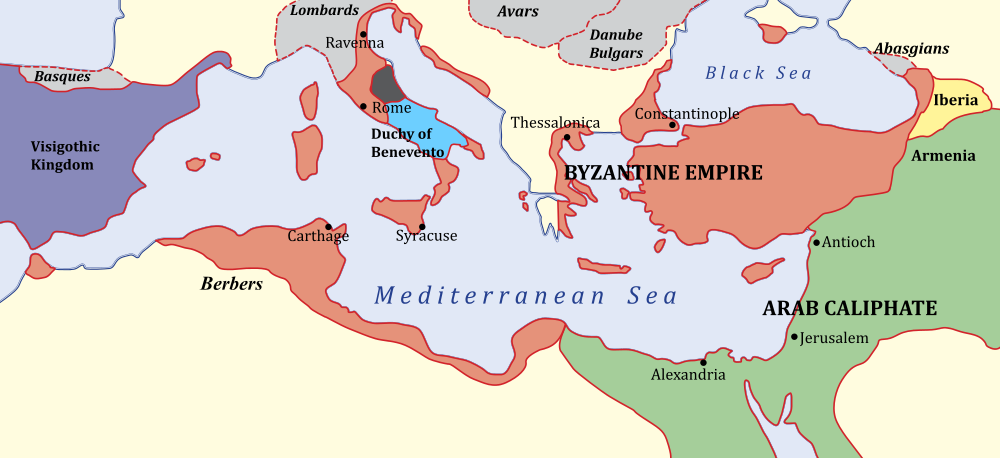
\includegraphics[height=5cm]{images/byzantium650.png}};
        \node (byzantium) at (2.4,3) {Byzantium/Constantinople/Istanbul};
        \draw [-Stealth,line width=4pt] (byzantium) -- (1.9,1.2);
    \end{tikzpicture}
    {\scriptsize Source: \url{https://commons.wikimedia.org/wiki/File:Byzantiumby650AD.svg}}\\[1em]
    \textbf{``Byzantine''} has long been used for ``excessively complicated, bureaucratic, devious'' (e.g.\ \emph{``the Byzantine tax law''})
\end{frame}
\inlineslide{s:byzantine-empire}{}\label{l:byzantine-empire}

\subsection{Describing nodes and network behaviour}\label{sec:system-behaviour}

When designing a distributed algorithm, a \emph{system model} is how we specify our assumptions about what faults may occur.

\begin{frame}
    \label{s:system-model}
    \frametitle{System models}
    We have seen two thought experiments:
    \begin{itemize}
        \item Two generals problem: a model of networks
        \item Byzantine generals problem: a model of node behaviour
    \end{itemize}
    In real systems, both nodes and networks may be faulty!\\[2em]\pause
    Capture assumptions in a \textbf{system model} consisting of:
    \begin{itemize}
        \item Network behaviour (e.g.\ message loss)
        \item Node behaviour (e.g.\ crashes)
        \item Timing behaviour (e.g.\ latency)
    \end{itemize}
    Choice of models for each of these parts.
\end{frame}
\inlineslide{s:system-model}{}\label{l:system-model}

Let's start with the network.
No network is perfectly reliable: even in carefully engineered systems with redundant network links, things can go wrong \citep{Bailis:2014jx}.
Someone might accidentally unplug the wrong network cable.
Sharks and cows have both been shown to cause damage and interruption to long-distance networks (see links on \autoref{l:shark-bite}).
Or a network may be temporarily overloaded, perhaps by accident or perhaps due to a denial-of-service attack.
Any of these can cause messages to be lost.

\begin{frame}
    \label{s:shark-bite}
    \frametitle{Networks are unreliable}
    % Source for network-cable.jpg: https://pixabay.com/photos/modem-antenna-wire-cable-router-5436144/
    % (Royalty-free, no attribution required)
    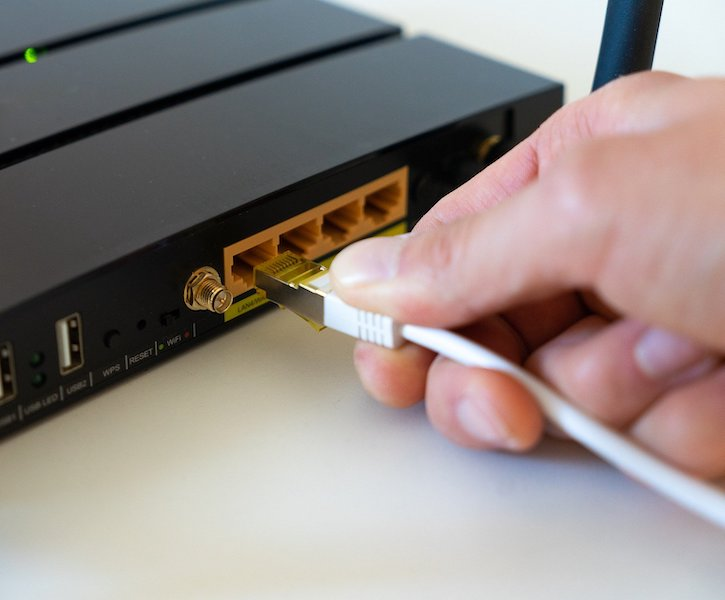
\includegraphics[height=4cm]{images/network-cable.jpg}
    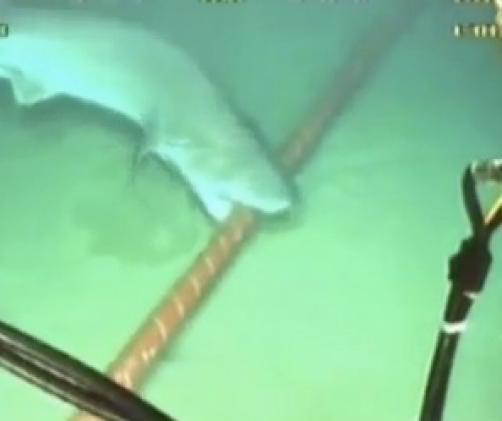
\includegraphics[height=4cm]{images/shark-bite.jpg}\\[1em]
    In the sea, sharks bite fibre optic cables \\
    {\scriptsize\url{https://slate.com/technology/2014/08/shark-attacks-threaten-google-s-undersea-internet-cables-video.html}}\\[1em]
    On land, cows step on the cables \\
    {\scriptsize\url{https://twitter.com/uhoelzle/status/1263333283107991558}}
\end{frame}
\inlineslide{s:shark-bite}{}\label{l:shark-bite}

In a system model, we take a more abstract view, which saves us from the details of worrying about sharks and cows.
Most distributed algorithms assume that the network provides bidirectional message-passing between pairs of nodes, also known as \emph{point-to-point} or \emph{unicast} communication.
Real networks do sometimes allow \emph{broadcast} or \emph{multicast} communication (sending a packet to many recipients at the same time, which is used e.g.\ for discovering a printer on a local network), but broadly speaking, assuming unicast-only is a good model of the Internet today.
Later, in \autoref{sec:broadcast}, we will explore how to implement broadcast on top of unicast communication.

We can then choose how reliable we want to assume these links to be.
Most algorithms assume one of the three choices listed on \autoref{l:model-network}.

\begin{frame}
    \label{s:model-network}
    \frametitle{System model: network behaviour}
    Assume bidirectional \textbf{point-to-point} communication between two nodes, with one of:\pause
    \begin{itemize}
        \item \textbf{Reliable} (perfect) links:\\
            A message is received if and only if it is sent.\tikz[remember picture]\node (reliable) {};\\
            Messages may be reordered.\pause
        \item \textbf{Fair-loss} links:\\
            Messages may be lost, duplicated, or reordered.\tikz[remember picture]\node (fairloss) {};\\
            If you keep retrying, a message eventually gets through.\pause
        \item \textbf{Arbitrary} links (active adversary):\\
            A malicious adversary may interfere with messages\tikz[remember picture]\node (arbitrary) {};\\
            (eavesdrop, modify, drop, spoof, replay).\\[1em]
    \end{itemize}\pause
    \textbf{Network partition}: some links dropping/delaying all messages for extended period of time
    \begin{tikzpicture}[remember picture,overlay]
        \draw<6-> [-Stealth,red,line width=4pt] (fairloss.north) .. controls +(1.6,0) and +(1.6,0) ..
            node [right,red,align=left] {retry +\\dedup} (reliable);
        \draw<7> [-Stealth,red,line width=4pt] (arbitrary) .. controls +(1.6,0) and +(1.6,0) ..
            node [right,red,align=left] {TLS} (fairloss.south);
    \end{tikzpicture}
\end{frame}
\inlineslide{s:model-network}{}\label{l:model-network}

Interestingly, it is possible to convert some types of link into others.
For example, if we have a fair-loss link, we can turn it into a reliable link by continually retransmitting lost messages until they are finally received, and by filtering out duplicated messages on the recipient side.
The fair-loss assumption means that any \emph{network partition} (network interruption) will last only for a finite period of time, but not forever.
Provided that the sender does not crash, we can guarantee that every message will eventually be received by retrying indefinitely.
However, if the sender crashes before the message gets through, it can no longer retry, and so the message will be lost.

Of course, any messages sent during a network partition will only be received after the interruption is repaired, which may take a long time, but the definitions on \autoref{l:model-network} do not say anything about network delay or latency.
We will get to that topic on \autoref{l:model-synchrony}.

The TCP protocol, which we discussed briefly in \autoref{sec:networking}, performs this kind of retry and deduplication at the network packet level.
However, TCP is usually configured with a timeout, so it will give up and stop retrying after a certain time, typically on the order of one minute.
To overcome network partitions that last for longer than this duration, a separate retry and deduplication mechanism needs to be implemented in addition to that provided by TCP.

\supervision{
    Say you have a client-server RPC system in which a client repeats an RPC request until it receives a response.
    How could the server deduplicate the requests?
}{
    When the server receives several identical requests, it needs to somehow determine whether they are duplicates, or whether the client really wanted the action to take place several times.
    One solution is for the client to attach a unique identifier to each distinct request, and to include the same identifier in all retries of that request.
    The server can then keep track of all request identifiers it has processed, and ignore any requests with identifiers it has already seen.
    This approach has the effect of making the RPC \emph{idempotent}, which we will discuss further in a later lecture.
}

An arbitrary link is an accurate model for communication over the Internet: whenever your communication is routed through a network (be it a coffee shop wifi or an Internet backbone network), the operator of that network can potentially interfere with and manipulate your network packets in arbitrary ways.
Someone who manipulates network traffic is also known as an \emph{active adversary}.
Fortunately, it is \emph{almost} possible to turn an arbitrary link into a fair-loss link using cryptographic techniques.
The \emph{Transport Layer Security} (TLS) protocol, which provides the ``s'' for ``secure'' in \verb|https://|, prevents an active adversary from eavesdropping, modifying, spoofing, or replaying traffic.

The only thing that TLS cannot prevent is the adversary dropping (blocking) communication.
Thus, an arbitrary link can be converted into a fair-loss link only if we assume that the adversary does not block communication forever.
In some networks, it might be possible to route around the interrupted network link, but this is not always the case.

Next, we consider different options for how nodes might behave.

\begin{frame}
    \label{s:model-nodes}
    \frametitle{System model: node behaviour}
    Each node executes a specified algorithm,\\assuming one of the following:
    \begin{itemize}
        \item \textbf{Crash-stop} (fail-stop):\\
            A node is faulty if it crashes (at any moment).\\
            After crashing, it stops executing forever.\pause
        \item \textbf{Crash-recovery} (fail-recovery):\\
            A node may crash at any moment, losing its in-memory state.
            It may resume executing sometime later.\\
            Data stored on disk survives the crash.\pause
        \item \textbf{Byzantine} (fail-arbitrary):\\
            A node is faulty if it deviates from the algorithm.\\
            Faulty nodes may do anything, including crashing or malicious behaviour.\\[1em]
    \end{itemize}
    A node that is not faulty is called \textbf{``correct''}
\end{frame}
\inlineslide{s:model-nodes}{}\label{l:model-nodes}

% Some distinguish between crash failures (cannot distinguish from slowness)
% and fail-stop (can detect accurately whether node has failed)
% https://twitter.com/lindsey/status/1465082487730700290

% Cachin et al. (page 17) define the following classes of *algorithm* (not of fault!):
% 1. fail-stop algorithms, designed under the assumption that processes can fail by
% crashing but the crashes can be reliably detected by all the other processes;
% 2. fail-silent algorithms, where process crashes can never be reliably detected;
% 3. fail-noisy algorithms, where processes can fail by crashing and the crashes can
% be detected, but not always in an accurate manner (accuracy is only eventual);

In the \emph{crash-stop} model, we assume that after a node crashes, it never recovers.
This is a reasonable model for an unrecoverable hardware fault, or when a phone is dropped in the river.
With a software crash, the crash-stop model might seem unrealistic, because we can just restart the node, after which it will recover.
Nevertheless, some algorithms assume a crash-stop model, since that makes the algorithm simpler than explicitly handling recovery after a crash.
In this case, a node that crashes and recovers would have to re-join the system as a new node.

Alternatively, the \emph{crash-recovery} model explicitly allows nodes to restart and resume processing after a crash.
When a node crashes and restarts, we assume that all of its in-memory state is lost, but any data it has stored persistently on disk is preserved.
The model makes no assumptions about how long it may take for a crashed node to recover, and it is possible for a crashed node to never recover.

Finally, the \emph{Byzantine} model is the most general model of node behaviour: as in the Byzantine generals problem, a faulty node may not only crash, but also deviate from the specified algorithm in arbitrary ways, including exhibiting malicious behaviour.
A bug in the implementation of a node could also be classed as a Byzantine fault.
However, if all of the nodes are running the same software, they will all have the same bug, and so any algorithm that is predicated on less than one third of nodes being Byzantine-faulty will not be able to tolerate such a bug.
In principle, we could try using several different implementations of the same algorithm, but this is rarely a practical option.
We therefore usually reserve the term \emph{Byzantine} when referring to deliberate deviation from the protocol, and not for bugs.

In the case of the network, it was possible to convert one model to another using generic protocols.
This is not the case with the different models of node behaviour.
For instance, an algorithm designed for a crash-recovery system model may look very different from a Byzantine algorithm.

% TODO: Dimitra Giantsidi's "Recipe" paper converts a CFT algorithm to BFT using TEEs. Paper not published yet, see Papers for draft

\begin{frame}
    \label{s:model-synchrony}
    \frametitle{System model: timing assumptions}
    Assume one of the following for network and nodes:
    \begin{itemize}
        \item \textbf{Synchronous}:\\
            Message latency no greater than a known upper bound.\\
            Nodes execute algorithm at a known speed.\pause
        \item \textbf{Partially synchronous}:\\
            The system is asynchronous for some finite (but unknown) periods of time, synchronous otherwise.\pause
        \item \textbf{Asynchronous}:\\
            Messages can be delayed arbitrarily.\\
            Nodes can pause execution arbitrarily.\\
            No timing guarantees at all.\\[1em]
    \end{itemize}
    \textbf{Note}: other parts of computer science use the terms ``synchronous'' and ``asynchronous'' differently.
\end{frame}
\inlineslide{s:model-synchrony}{}\label{l:model-synchrony}

The third part of a system model is the synchrony assumption, which is about timing.
The three choices we can make here are \emph{synchronous}, \emph{asynchronous}, or \emph{partially synchronous} \citep{Dwork:1988dr}.

\begin{mdframed}
Note: confusingly, these terms are also used with a different meaning in other contexts.
For example, in the context of RPC and I/O operations, ``synchronous'' often means ``the caller blocks/waits for the operation to complete'', and ``asynchronous'' means ``the caller continues executing after issuing a request, without waiting for the result''.
It's unfortunate that the same words are used with different meanings, but since these terms are widely used in the literature, we will stick with the standard terminology.
\end{mdframed}

A synchronous system is what we would love to have: a message sent over the network never takes longer than some known maximum latency, and nodes always execute their algorithm at a predictable speed.
Many problems in distributed computing are much easier if you assume a synchronous system.
And it is tempting to assume synchrony, because networks and nodes are well-behaved \emph{most of the time}, and so this assumption is often true.

Unfortunately, \emph{most of the time} is not the same as \emph{always}, and algorithms designed for a synchronous model often fail catastrophically if the assumptions of bounded latency and bounded execution speed are violated, even just for a short while, and even if this happens rarely.
And in practical systems, there are many reasons why network latency or execution speed may sometimes vary wildly, see \autoref{l:timing-violations}.

\begin{frame}
    \label{s:timing-violations}
    \frametitle{Violations of synchrony in practice}
    Networks usually have quite predictable latency, which can occasionally increase:
    \begin{itemize}
        \item Message loss requiring retry
        \item Congestion/contention causing queueing
        \item Network/route reconfiguration\\[1em]
    \end{itemize}\pause
    Nodes usually execute code at a predictable speed, with occasional pauses:
    \begin{itemize}
        \item Operating system scheduling issues, e.g.\ priority inversion
        \item Stop-the-world garbage collection pauses
        \item Page faults, swap, thrashing
    \end{itemize}
    Real-time operating systems (RTOS) provide scheduling guarantees, but most distributed systems do not use RTOS
\end{frame}
\inlineslide{s:timing-violations}{}\label{l:timing-violations}

The other extreme is an asynchronous model, in which we make no timing assumptions at all: we allow messages to be delayed arbitrarily in the network, and we allow arbitrary differences in nodes' processing speeds (for example, we allow one node to pause execution while other nodes continue running normally).
Algorithms that are designed for an asynchronous model are typically very robust, because they are unaffected by any temporary network interruptions or spikes in latency.

Unfortunately, some problems in distributed computing are impossible to solve in an asynchronous model, and therefore we have the \emph{partially synchronous} model as a compromise.
In this model, we assume that our system is synchronous and well-behaved most of the time, but occasionally it may flip into asynchronous mode in which all timing guarantees are off, and this can happen unpredictably.
The partially synchronous model is good for many practical systems, but using it correctly requires care.

There are many reasons why a system may violate synchrony assumptions.
We have already talked about latency increasing without bound if messages are lost and retransmitted, especially if we have to wait for a network partition to be repaired before the messages can get through.
Another reason for latency increases in a network is congestion resulting in queueing of packets in switch buffers.
Network reconfiguration can also cause large delays: even within a single datacenter, there have been documented cases of packets being delayed for more than a minute \citep{Imbriaco:2012tx}.

We might expect that the speed at which nodes execute their algorithms is constant: after all, an instruction generally takes a fixed number of CPU clock cycles, and the clock speed doesn't vary much.
However, even on a single node, there are many reasons why a running program may unexpectedly get paused for significant amounts of time.
Scheduling in the operating system can preempt a running thread and leave it paused while other programs run, especially on a machine under heavy load.
A real problem in memory-managed languages such as Java is that when the garbage collector runs, it needs to pause all running threads from time to time (this is known as a \emph{stop-the-world} garbage collection pause).
On large heaps, such pauses can be as long as several minutes \citep{Thompson:2013}!
Page faults are another reason why a thread may get suspended, especially when there is not much free memory left.

Threads can and will get preempted even at the most inconvenient moments, anywhere in a program.
In a distributed system, this is particularly problematic, because for one node, time appears to ``stand still'' while it is paused, and during this time all other nodes continue executing their algorithms normally.
Other nodes may even notice that the paused node is not responding, and assume that it has crashed.
After a while, the paused node resumes processing, without even realising that it was paused for a significant period of time.

Note that these execution pauses are not the same as a crash and restart as discussed on \autoref{l:model-nodes}.
When an executing process or thread is paused, it normally does not notice it has been paused, unless it regularly checks the system clock to measure elapsed time.
On the other hand, a restart is explicitly handled by the program, since its in-memory state is lost during the crash, and on restart it may load its persistent state from disk.

Combined with the many reasons for variable network latency, this means that in practical systems, it is very rarely safe to assume a synchronous system model.
Most distributed algorithms need to be designed for the asynchronous or partially synchronous model.

\begin{frame}
    \label{s:model-summary}
    \frametitle{System models summary}
    For each of the three parts, pick one:\\
    \begin{itemize}
        \item \textbf{Network:}\\
            reliable, fair-loss, or arbitrary\\[1em]
        \item \textbf{Nodes:}\\
            crash-stop, crash-recovery, or Byzantine\\[1em]
        \item \textbf{Timing:}\\
            synchronous, partially synchronous, or asynchronous\\[1em]
    \end{itemize}
    This is the basis for any distributed algorithm.\\
    If your assumptions are wrong, all bets are off!
\end{frame}
\inlineslide{s:model-summary}{}\label{l:model-summary}

\subsection{Failure detectors}\label{sec:failure-detectors}

As highlighted on \autoref{l:why-distribute}, one reason for building distributed systems is to achieve higher reliability than is possible with a single computer.
We will now explore this idea further in the light of the system models we have discussed.

The first step towards tolerating faults is to detect faults, which is often done with a \emph{failure detector}.
(``Fault detector'' would be a more logical name, but ``failure detector'' is the conventional term.)
A failure detector usually detects crash faults.
Byzantine faults are not always detectable, although in some cases Byzantine behaviour does leave evidence that can be used to identify and exclude malicious nodes.

\begin{frame}
    \label{s:failure-detector}
    \frametitle{Failure detectors}
    \textbf{Failure detector}:\\algorithm that detects whether another node is faulty\\[1em]
    \textbf{Perfect failure detector}:\\labels a node as faulty if and only if it has crashed\\[1em]\pause
    \textbf{Typical implementation} for crash-stop/crash-recovery:\\
    send message, await response, label node as crashed if no reply within some timeout\\[1em]\pause
    \textbf{Problem}:\\cannot tell the difference between crashed node, temporarily
    unresponsive node, lost message, and delayed message\\[1em]
\end{frame}
\inlineslide{s:failure-detector}{}\label{l:failure-detector}

In most cases, a failure detector works by periodically sending messages to other nodes, and labelling a node as crashed if no response is received within the expected time.
Ideally, we would like a timeout to occur if and only if the node really has crashed (this is called a \emph{perfect failure detector}).
However, the two generals problem tells us that this is not a totally accurate way of detecting a crash, because the absence of a response could also be due to message loss or delay.

A perfect timeout-based failure detector exists only in a synchronous crash-stop system with reliable links; in a partially synchronous system, a perfect failure detector does not exist.
Moreover, in an asynchronous system, no timeout-based failure exists, since timeouts are meaningless in the asynchronous model.
However, there is a useful failure detector that exists in partially synchronous systems: the \emph{eventually perfect failure detector} \citep{Chandra:1996}.

\begin{frame}
    \label{s:eventual-detector}
    \frametitle{Failure detection and partial synchrony}
    Perfect timeout-based failure detector exists only in a synchronous crash-stop system with reliable links.\\[1em]
    \textbf{Eventually perfect failure detector}:
    \begin{itemize}
        \item May \emph{temporarily} label a node as crashed,\\ even though it is correct
        \item May \emph{temporarily} label a node as correct,\\ even though it has crashed
        \item But \emph{eventually}, labels a node as crashed\\ if and only if it has crashed\\[1em]
    \end{itemize}
    Reflects fact that detection is not instantaneous, and we may have spurious timeouts
\end{frame}
\inlineslide{s:eventual-detector}{}\label{l:eventual-detector}

We will see later how to use such a failure detector to design fault-tolerance mechanisms and to automatically recover from node crashes.
Using such algorithms it is possible to build systems that are highly available.

\supervision{\label{q:fifo-links}
    Reliable network links allow messages to be reordered.
    Give pseudocode for an algorithm that strengthens the properties of a reliable point-to-point link such that messages are received in the order they were sent (this is called a FIFO link), assuming an asynchronous crash-stop system model.
}{
    The sender attaches a sequence number to each message, and increments that number for each message sent.
    The recipient delivers messages in increasing order by sequence number.
    This may require buffering a message on the recipient side until messages with prior sequence numbers have arrived.

    \begin{algorithmic}
        \On{initialisation}
            \State [We have a separate copy of the following variables for each network link.]
            \State $\mathit{lastSent} := 0;\; \mathit{nextReceived} := 1;\; \mathit{buffer} := \{\}$
        \EndOn
        \State
        \On{request to send message $m$ over FIFO link}
            \State \textit{lastSent}++
            \State \textbf{send} $(m, \mathit{lastSent})$ via the underlying network link
        \EndOn
        \State
        \On{receiving $(m, n)$ via the underlying network link}
            \State $\mathit{buffer} := \mathit{buffer} \cup \{(m,n)\}$
            \While{$\exists m'.\; (m', \mathit{nextReceived}) \in \mathit{buffer}$}
                \State \textbf{deliver} $m'$ to the application
                \State \textit{nextReceived}++
            \EndWhile
        \EndOn
    \end{algorithmic}
}

\supervision{
    How do we need to change the algorithm from \autoref{q:fifo-links} if we assume a crash-recovery model instead of a crash-stop model?
}{
    When a node crashes and recovers, all of its in-memory state is lost.
    The sequence number algorithm maintains state in the form of the variables \textit{lastSent}, \textit{nextReceived}, and \textit{buffer}.
    This information needs to be preserved across crashes, so it must be maintained in non-volatile storage (e.g.\ on disk).

    Another issue is that a node may crash while in the process of sending or delivering a message.
    In that case, we will need to decide: does that message get sent/delivered after recovering from the crash?
    If so, the information about such in-progress operations will also need to be written to non-volatile storage.
}

\section{Time, clocks, and ordering of events}\label{sec:time}

\begin{frame}
    \begin{center}
        {\Large{\color{darkblue}{Time, clocks, and ordering of events}}} \\[2em]
        \mydetails
    \end{center}
\end{frame}

Let's start with a riddle, which will be resolved later in this lecture.

\begin{frame}
    \label{s:mystery}
    \frametitle{A detective story}
    In the night from 30 June to 1 July 2012 (UK time), many online services and systems around the world crashed simultaneously.\\[1em]
    Servers locked up and stopped responding.\\[1em]
    Some airlines could not process any reservations or check-ins for several hours.\\[1em]
    What happened?
\end{frame}
\inlineslide{s:mystery}{}\label{l:mystery}

In this lecture we will look at the concept of time in distributed systems.
We have already seen that our assumptions about timing form a key part of the system model that distributed algorithms rely on.
For example, timeout-based failure detectors need to measure time to determine when a timeout has elapsed.
Operating systems rely extensively on timers and time measurements in order to schedule tasks, keep track of CPU usage, and many other purposes.
Applications often want to record the time and date at which events occurred: for example, when debugging an error in a distributed system, timestamps are helpful for debugging, since they allow us to reconstruct which things happened around the same time on different nodes.
All of these require more or less accurate measurements of time.

\begin{frame}
    \label{s:clocks-intro}
    \frametitle{Clocks and time in distributed systems}
    Distributed systems often need to measure time, e.g.:
    \begin{itemize}
        \item Schedulers, timeouts, failure detectors, retry timers\pause
        \item Performance measurements, statistics, profiling\pause
        \item Log files \& databases: record when an event occurred\pause
        \item Data with time-limited validity (e.g.\ cache entries)\pause
        \item Determining order of events across several nodes\\[1em]\pause
    \end{itemize}
    We distinguish two types of clock:
    \begin{itemize}
        \item \textbf{physical clocks}: count number of seconds elapsed
        \item \textbf{logical clocks}: count events, e.g.\ messages sent\\[1em]
    \end{itemize}\pause
    \textbf{NB.} Clock in digital electronics (oscillator)\\$\neq$ clock in distributed systems (source of \textbf{timestamps})
\end{frame}
\inlineslide{s:clocks-intro}{}\label{l:clocks-intro}

% Demo: load www.cst.cam.ac.uk in browser, open developer tools and view certificate expiry date
% Also run `dig www.cst.cam.ac.uk` in a terminal and see how the TTL counts down

\subsection{Physical clocks}\label{sec:physical-clocks}

\emph{Physical clocks} measure the time in seconds.
They include analogue/mechanical clocks based on pendulums or similar mechanisms, and digital clocks based e.g.\ on a vibrating quartz crystal.
Quartz clocks are found in most wristwatches, in every computer and mobile phone, in microwave ovens that display the time, and many other everyday objects.
Physical clocks are sometimes also called wall clocks, even though they need not be attached to an actual wall.

\begin{frame}
    \label{s:quartz-clocks}
    \frametitle{Quartz clocks}
    \begin{columns}
        \begin{column}{0.5\textwidth}
            \begin{itemize}
                \item Quartz crystal laser-trimmed to mechanically resonate at a specific frequency
                \item Piezoelectric effect: mechanical force $\Leftrightarrow$ electric field
                \item Oscillator circuit produces signal at resonant frequency
                \item Count number of cycles to measure elapsed time
            \end{itemize}
        \end{column}
        \begin{column}{0.5\textwidth}
            
\includegraphics[width=\textwidth]{images/quartz-crystal.jpg}\\[1em]
            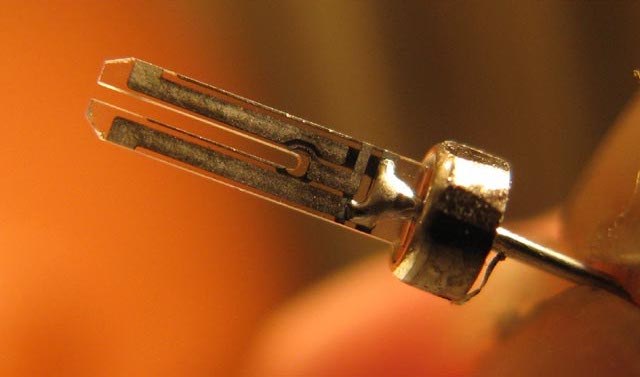
\includegraphics[width=\textwidth]{images/quartz-tuningfork.jpg}
        \end{column}
    \end{columns}
\end{frame}
\inlineslide{s:quartz-clocks}{}\label{l:quartz-clocks}
% Crystal image: https://pixabay.com/photos/rock-crystal-clear-to-white-gem-top-1603480/ (no attribution required)
% Tuning fork: https://commons.wikimedia.org/wiki/File:Inside_QuartzCrystal-Tuningfork.jpg (public domain)

Quartz clocks are cheap, but they are not totally accurate.
Due to manufacturing imperfections, some clocks run slightly faster than others.
Moreover, the oscillation frequency varies with the temperature.
Typical quartz clocks are tuned to be quite stable around room temperature, but significantly higher or lower temperatures slow down the clock.
The rate by which a clock runs fast or slow is called \emph{drift}.

\pagebreak[3]
\begin{frame}
    \label{s:quartz-drift}
    \frametitle{Quartz clock error: drift}
    \begin{itemize}
        \item One clock runs slightly fast, another slightly slow
        \item Drift measured in \textbf{parts per million} (ppm)
        \item 1~ppm = 1~microsecond/second = 86~ms/day = 32~s/year
        \item Most computer clocks correct within $\approx 50$~ppm\\[1em]
        % 50 ppm is about half an hour of drift per year
    \end{itemize}
    \begin{columns}
        \begin{column}{0.2\textwidth}
            Temperature significantly affects drift
        \end{column}
        \begin{column}{0.75\textwidth}
            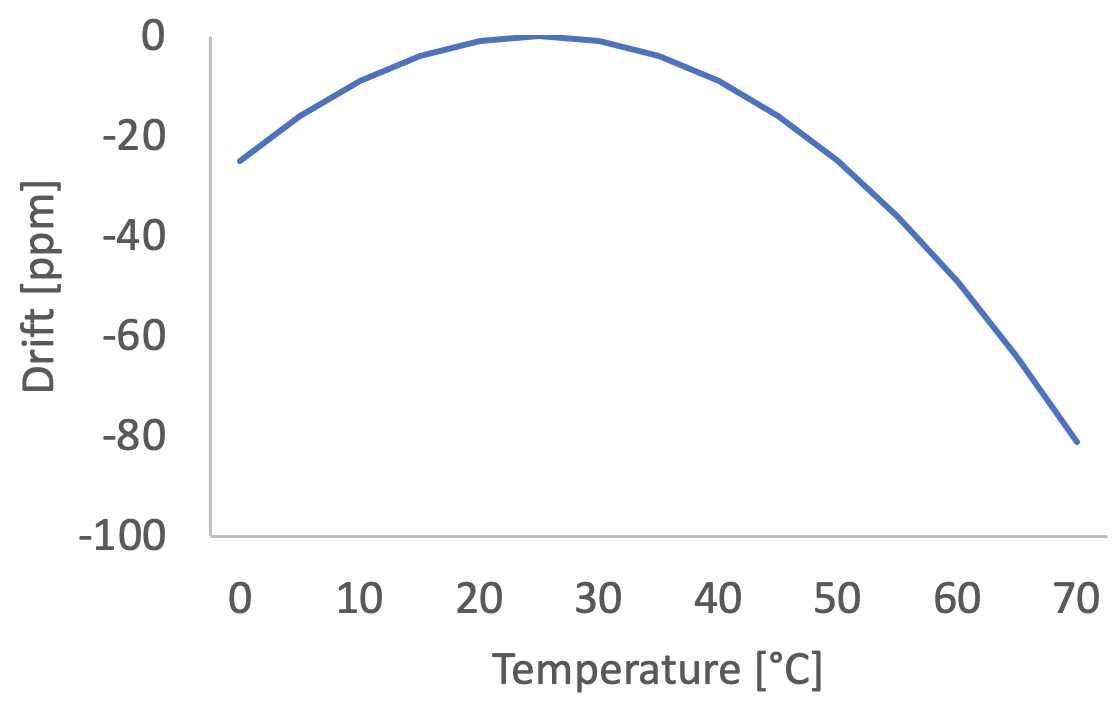
\includegraphics[width=\textwidth]{images/quartz-drift.png}
        \end{column}
    \end{columns}
\end{frame}
\inlineslide{s:quartz-drift}{}\label{l:quartz-drift}

When greater accuracy is required, atomic clocks are used.
These clocks are based on quantum-mechanical properties of certain atoms, such as caesium or rubidium.
In fact, the time unit of \emph{one second} in the International System of Units (SI) is defined to be exactly 9,192,631,770 periods of a particular resonant frequency of the caesium-133 atom.

\begin{frame}
    \label{s:atomic-clocks}
    \frametitle{Atomic clocks}
    \begin{columns}
        \begin{column}{0.5\textwidth}
            \begin{itemize}
                \item Caesium-133 has a resonance (``hyperfine transition'') at $\approx 9$~GHz
                \item Tune an electronic oscillator to that resonant frequency
                \item 1 second = 9,192,631,770 periods of that signal
                \item Accuracy $\approx 1 \text{ in } 10^{-14}$ (1 second in 3 million years)
                \item Price $\approx$ {\textsterling}20,000 (?)\\ (can get cheaper rubidium clocks for $\approx$ {\textsterling}1,000)
            \end{itemize}
        \end{column}
        \begin{column}{0.5\textwidth}
            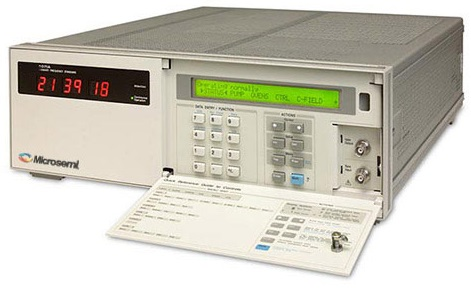
\includegraphics[width=\textwidth]{images/atomic-clock.jpg}\\[1em]
            \scriptsize\url{https://www.microsemi.com/product-directory/cesium-frequency-references/4115-5071a-cesium-primary-frequency-standard}
        \end{column}
    \end{columns}
\end{frame}
\inlineslide{s:atomic-clocks}{}\label{l:atomic-clocks}

Another high-accuracy method of obtaining the time is to rely on the GPS satellite positioning system, or similar systems such as Galileo or GLONASS.
These systems work by having several satellites orbiting the Earth and broadcasting the current time at very high resolution.
Receivers measure the time it took the signal from each satellite to reach them, and use this to compute their distance from each satellite, and hence their location.
By connecting a GPS receiver to a computer, it is possible to obtain a clock that is accurate to within a fraction of a microsecond, provided that the receiver is able to get a clear signal from the satellites.
In a datacenter, there is generally too much electromagnetic interference to get a good signal, so a GPS receiver requires an antenna on the roof of the datacenter building.

\begin{frame}
    \label{s:gps-time}
    \frametitle{GPS as time source}
    \begin{columns}
        \begin{column}{0.5\textwidth}
            \begin{itemize}
                \item 31 satellites, each carrying an atomic clock
                \item satellite broadcasts current time and location
                \item calculate position from speed-of-light delay between satellite and receiver
                \item corrections for atmospheric effects, relativity, etc.
                \item in datacenters, need antenna on the roof
            \end{itemize}
        \end{column}
        \begin{column}{0.5\textwidth}
            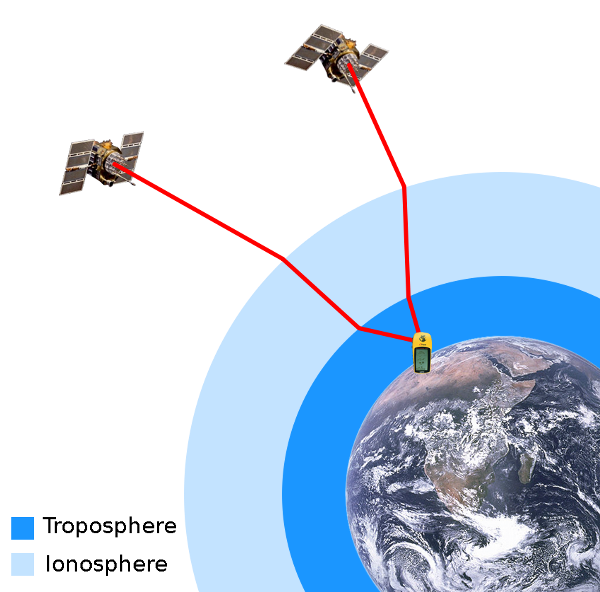
\includegraphics[width=\textwidth]{images/gps-satellites.png}\\[1em]
            \scriptsize\url{https://commons.wikimedia.org/wiki/File:Gps-atmospheric-efects.png}
        \end{column}
    \end{columns}
\end{frame}
\inlineslide{s:gps-time}{}\label{l:gps-time}

The system of time measurement based on atomic clocks (International Atomic Time, TAI) works well, but it is disconnected from our everyday perception of time, which is based around sunrise and sunset.
One rotation of planet Earth around its own axis does not take exactly $24 \times 60 \times 60 \times \text{9,192,631,770}$ periods of caesium-133's resonant frequency.
In fact, the speed of rotation of the planet is not even constant: it fluctuates due to the effects of tides, earthquakes, glacier melting, and some unexplained factors.
We now have a problem: we have two different definitions of time~-- one based on quantum mechanics, the other based on astronomy~-- and those two definitions don't match up precisely.

The solution is \emph{Coordinated Universal Time} (UTC), which is based on atomic time, but includes corrections to account for variations in the Earth's rotation.
In everyday life we use our local \emph{time zone}, which is specified as an offset to UTC.

The UK's local time zone is called \emph{Greenwich Mean Time} (GMT) in winter, and \emph{British Summer Time} (BST) in summer, where GMT is defined to be equal to UTC, and BST is defined to be UTC~+~1~hour.
Confusingly, the term \emph{Greenwich Mean Time} was originally used to refer to mean solar time on the Greenwich meridian, i.e.\ it used to be defined in terms of astronomy, while now it is defined in terms of atomic clocks.
Today, the term \emph{UT1} is used to refer to mean solar time at 0{\textdegree} longitude.

\begin{frame}
    \label{s:utc}
    \frametitle{Coordinated Universal Time (UTC)}
    \begin{columns}
        \begin{column}{0.7\textwidth}
            \textbf{Greenwich Mean Time} (GMT, solar time): it's noon when the sun is in the south, as seen from the Greenwich meridian\\[1em]
            \uncover<2->{\textbf{International Atomic Time} (TAI): 1 day is
            $24 \times 60 \times 60 \times \text{9,192,631,770}$ periods of caesium-133's resonant frequency\\[1em]}
            \uncover<3->{\textbf{Problem}: speed of Earth's rotation is not constant\\[1em]}
            \uncover<4->{\textbf{Compromise}: UTC is TAI with corrections to account for Earth rotation\\[1em]}
            \uncover<5->{\textbf{Time zones} and \textbf{daylight savings time} are offsets to UTC}
        \end{column}
        \begin{column}{0.3\textwidth}
            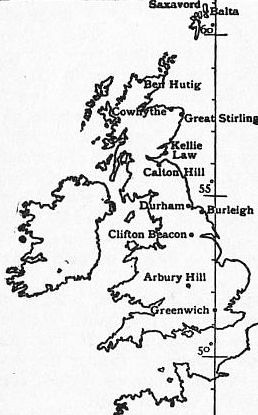
\includegraphics[width=\textwidth]{images/greenwich-meridian.jpg}
        \end{column}
    \end{columns}
\end{frame}
\inlineslide{s:utc}{}\label{l:utc}
% Image source: https://commons.wikimedia.org/wiki/File:Britannica_Figure_of_the_Earth.jpg (public domain)

% Earth has slowed down, so there might not be another leap second for a while:
% https://fanf.dreamwidth.org/133823.html

% TODO: leap seconds to be discontinued by 2035!
% https://www.theguardian.com/world/2022/nov/18/do-not-adjust-your-clock-scientists-call-time-on-the-leap-second

The difference between UTC and TAI is that UTC includes \emph{leap seconds}, which are added as needed to keep UTC roughly in sync with the rotation of the Earth.

\begin{frame}
    \label{s:leap-seconds}
    \frametitle{Leap seconds}
    Every year, on 30 June and 31 December at 23:59:59 UTC, one of three things happens:
    \begin{itemize}
        \item The clock immediately jumps forward to 00:00:00, skipping one second (\textbf{negative leap second})
        \item The clock moves to 00:00:00 after one second, as usual
        \item The clock moves to 23:59:60 after one second, and then moves to 00:00:00 after one further second\\
            (\textbf{positive leap second})
    \end{itemize}
    This is announced several months beforehand.
    \begin{center}
        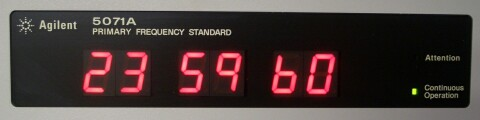
\includegraphics[width=8cm]{images/leap-second.jpg}
        \scriptsize\url{http://leapsecond.com/notes/leap-watch.htm}
    \end{center}
\end{frame}
\inlineslide{s:leap-seconds}{}\label{l:leap-seconds}

Due to leap seconds, it is not true that an hour always has 3600 seconds, and a day always has 86,400 seconds.
In the UTC timescale, a day can be 86,399 seconds, 86,400 seconds, or 86,401 seconds long due to a leap second.
This complicates software that needs to work with dates and times.

\begin{frame}
    \label{s:time-representation}
    \frametitle{How computers represent timestamps}
    Two most common representations:
    \begin{itemize}
        \item \textbf{Unix time}: number of seconds since 1 January 1970 00:00:00 UTC (the ``epoch''), \emph{not counting leap seconds}
        \item \textbf{ISO 8601}: year, month, day, hour, minute, second, and timezone offset relative to UTC\\
            example: \texttt{\timestampexample}\\[1em]
    \end{itemize}\pause
    Conversion between the two requires:
    \begin{itemize}
        \item Gregorian calendar: 365 days in a year, except leap years\\
            \texttt{(year \% 4 == 0 \&\& (year \% 100 != 0 ||}\\
            \texttt{~~~~~~~~~~~~~~~~~~~year \% 400 == 0))}
        \item Knowledge of past and future leap seconds\dots?!
    \end{itemize}
\end{frame}
\inlineslide{s:time-representation}{}\label{l:time-representation}

In computing, a \emph{timestamp} is a representation of a particular point in time.
Two representations of timestamps are commonly used: Unix time and ISO~8601.
For Unix time, zero corresponds to the arbitrarily chosen date of 1 January 1970, known as the \emph{epoch}.
There are minor variations: for example, Java's \verb|System.currentTimeMillis()| is like Unix time, but uses milliseconds rather than seconds.

To be correct, software that works with timestamps needs to know about leap seconds.
For example, if you want to calculate how many seconds elapsed between two timestamps, you need to know how many leap seconds were inserted between those two dates.
For dates that are more than about six months into the future, this is impossible to know, because the Earth's rotation has not happened yet!

The most common approach in software is to simply ignore leap seconds, pretend that they don't exist, and hope that the problem somehow goes away.
This approach is taken by Unix timestamps, and by the POSIX standard.
For software that only needs coarse-grained timings (e.g.\ rounded to the nearest day), this is fine, since the difference of a few seconds is not significant.

However, operating systems and distributed systems often \emph{do} rely on high-resolution timestamps for accurate measurements of time, where a difference of one second is very noticeable.
In such settings, ignoring leap seconds can be dangerous.
For example, say you have a Java program that twice calls \verb|System.currentTimeMillis()|, 500~ms apart, within a positive leap second (i.e.\ while the clock is saying 23:59:60).
What is the difference between those two timestamps going to be?
It can't be 500, since the \verb|currentTimeMillis()| clock does not account for leap seconds.
Does the clock stop, so the difference between the two timestamps is zero?
Or could the difference even be negative, so the clock runs backwards for a brief moment?
The documentation is silent about this question.
(The best solution is probably to use a \emph{monotonic clock} instead, which we introduce on \autoref{l:monotonic-clock}.)

Poor handling of the leap second on 30 June 2012 is what caused the simultaneous failures of many services on that day (\autoref{l:mystery}).
Due to a bug in the Linux kernel, the leap second had a high probability of triggering a livelock condition when running a multithreaded process \citep{Allen:2013,Minar:2012}.
Even a reboot did not fix the problem, but setting the system clock reset the bad state in the kernel.

\begin{frame}
    \label{s:leap-second-handling}
    \frametitle{How most software deals with leap seconds}
    \begin{columns}
        \begin{column}{0.7\textwidth}
            \textbf{By ignoring them!}\\[1em]
            \uncover<2->{However, OS and DistSys often need timings with sub-second accuracy.\\[1em]}
            \uncover<3->{30 June 2012: bug in Linux kernel caused livelock on leap second, causing many Internet services to go down\\[1em]}
            \uncover<4->{Pragmatic solution: ``\textbf{smear}'' (spread out) the leap second over the course of a day}
        \end{column}
        \begin{column}{0.3\textwidth}
            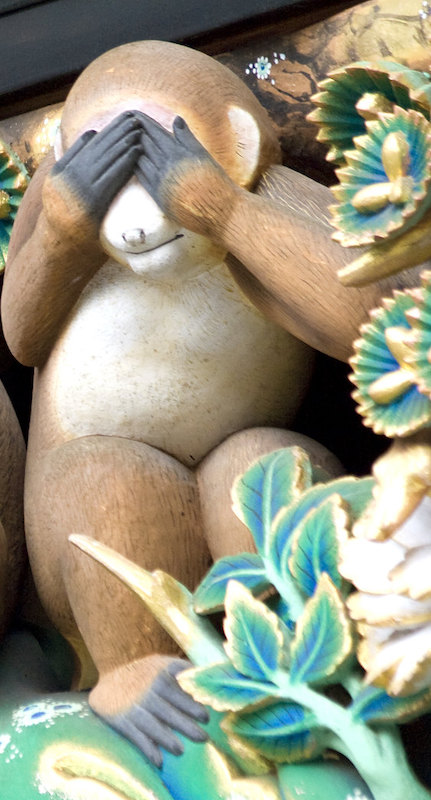
\includegraphics[width=\textwidth]{images/monkey.jpg}
            \scriptsize\url{https://www.flickr.com/photos/ru_boff/37915499055/}
        \end{column}
    \end{columns}
\end{frame}
\inlineslide{s:leap-second-handling}{}\label{l:leap-second-handling}

Today, some software handles leap seconds explicitly, while other programs continue to ignore them.
A pragmatic solution that is widely used today is that when a positive leap second occurs, rather than inserting it between 23:59:59 and 00:00:00, the extra second is spread out over several hours before and after that time by deliberately slowing down the clocks during that time (or speeding up in the case of a negative leap second).
This approach is called \emph{smearing} the leap second, and it is not without problems.
However, it is a pragmatic alternative to making all software aware of and robust to leap seconds, which may well be infeasible.

\supervision{
    Describe some problems that may arise from leap second smearing.
}{
    Measurements of time duration will be slightly wrong during the smearing period.
    For example, if the extra second is spread over 24 hours (12 hours before and 12 hours after the leap second), this amounts to an error of about 12~ppm in the rate at which clocks are running.
    However, many systems can tolerate this level of inaccuracy.

    A bigger problem is that if a timestamp from a smeared clock is compared with a non-smeared timestamp, there will be a spurious difference of up to half a second.
    For example, this could arise if two nodes with different smearing policies attempt to measure the network latency between them by sending one node's current timestamp as a message to the other node, and calculating the difference of timestamps when the message is received.
    The measured latency could even be negative.

    A similar problem arises (to a lesser degree) when comparing two timestamps from clocks that use different approaches to smearing.
    For example, some implementations of smearing spread the extra second over different periods of time.
    Also, different functions are used to interpolate across the leap second discontinuity: some systems use a linear functions, other use a cosine.
    There is no standardised approach to smearing.

    See \url{https://developers.google.com/time/smear} for some discussion.
    Our department's Markus Kuhn tried to get this standardised in 2006: \url{https://www.cl.cam.ac.uk/~mgk25/time/utc-sls/}
}

\newpage
\subsection{Clock synchronisation and monotonic clocks}\label{sec:clock-sync}

\begin{frame}
    \label{s:clock-sync}
    \frametitle{Clock synchronisation}
    Computers track physical time/UTC with a quartz clock\\
    (with battery, continues running when power is off)\\[1em]
    Due to \textbf{clock drift}, clock error gradually increases\\[1em]\pause
    \textbf{Clock skew}: difference between two clocks at a point in time\\[1em]\pause
    \textbf{Solution}: Periodically get the current time from a server that has a more
    accurate time source (atomic clock or GPS receiver)\\[1em]
    Protocols: Network Time Protocol (\textbf{NTP}),\\ Precision Time Protocol (\textbf{PTP})
\end{frame}
\inlineslide{s:clock-sync}{}\label{l:clock-sync}

Atomic clocks are too expensive and bulky to build into every computer and phone, so quartz clocks are used.
Since these clocks drift, they need adjustment from time to time, which is most commonly done using the \emph{Network Time Protocol} (NTP).
All mainstream operating systems have NTP clients built in.

\begin{frame}[plain]
    \label{s:ntp-config}
    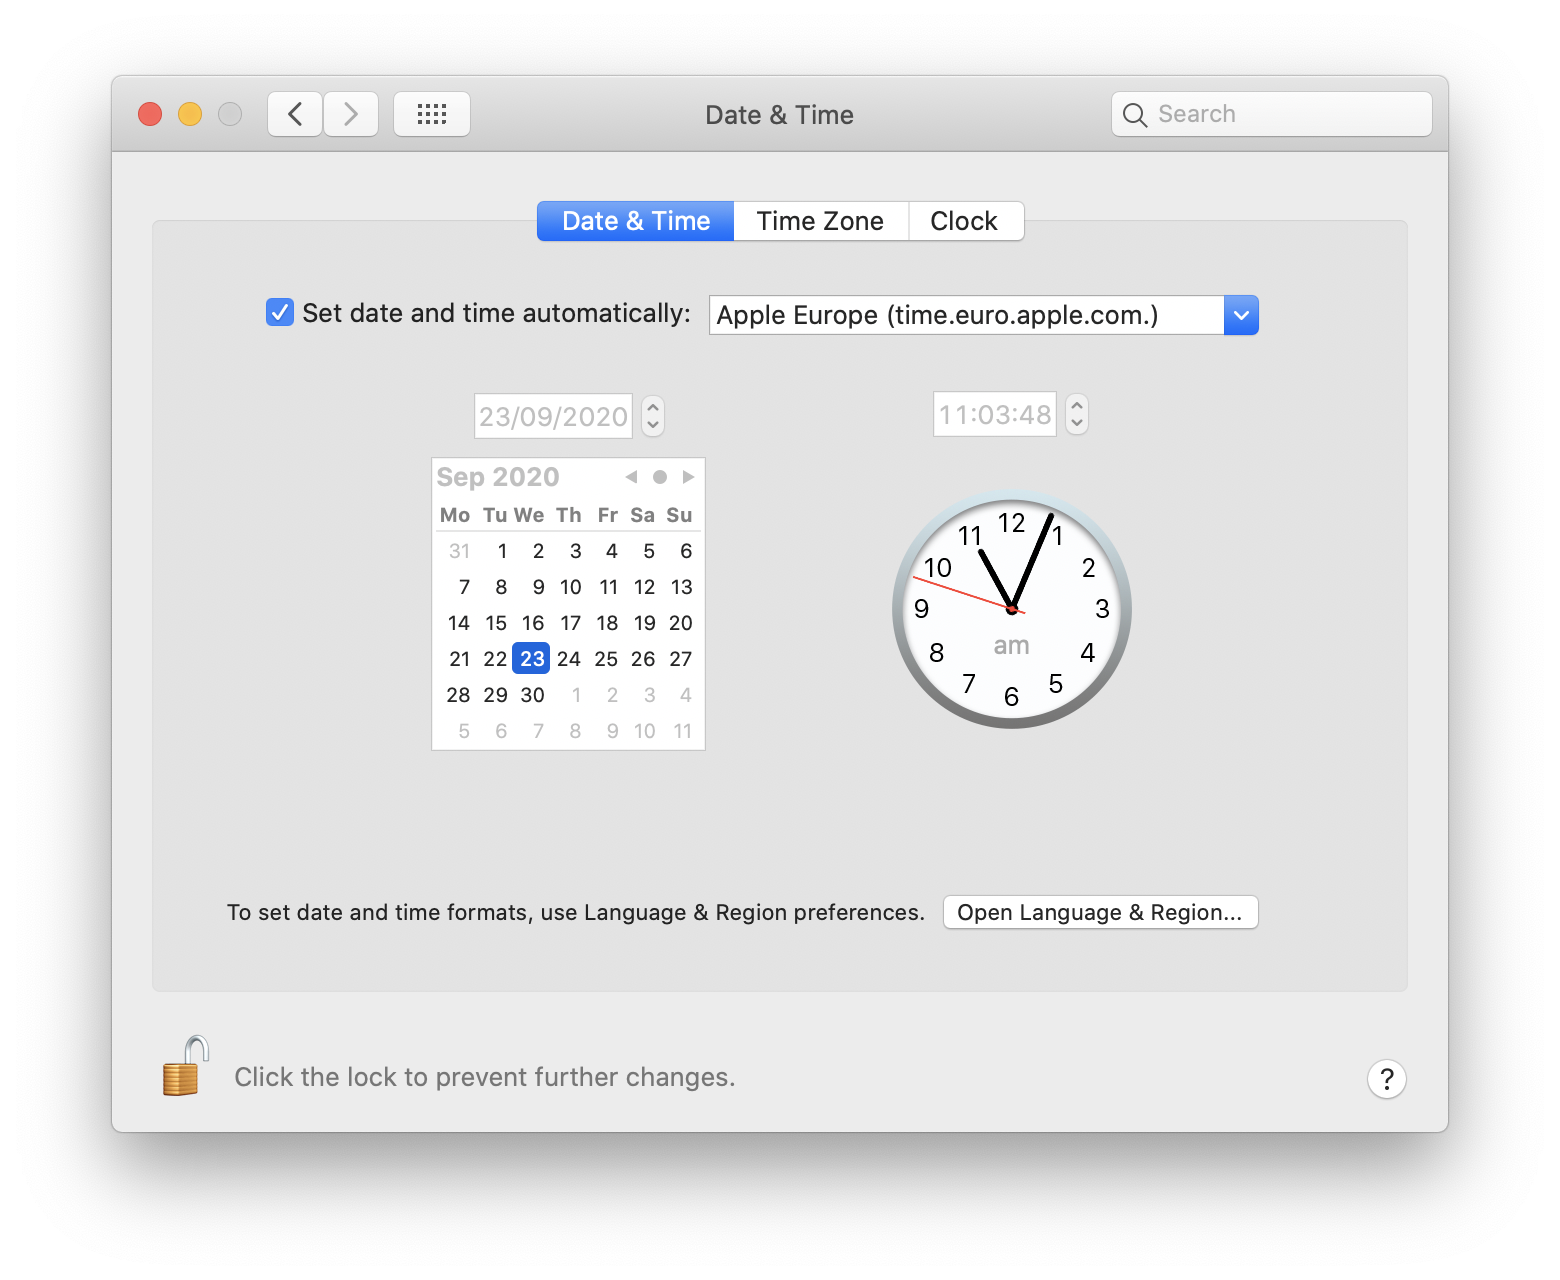
\includegraphics[height=\paperheight]{images/ntp-config.png}
\end{frame}
\inlineslide{s:ntp-config}{}\label{l:ntp-config}

\begin{frame}
    \label{s:ntp}
    \frametitle{Network Time Protocol (NTP)}
    Many operating system vendors run NTP servers,\\configure OS to use them by default\\[1em]\pause
    Hierarchy of clock servers arranged into \textbf{strata}:
    \begin{itemize}
        \item Stratum 0: atomic clock or GPS receiver
        \item Stratum 1: synced directly with stratum 0 device
        \item Stratum 2: servers that sync with stratum 1, etc.\\[1em]
    \end{itemize}\pause
    May contact multiple servers, discard outliers, average rest\\[1em]
    Makes multiple requests to the same server, use statistics to reduce random error due to variations in network latency\\[1em]
    Reduces clock skew to a few milliseconds in good network conditions, but can be much worse!
\end{frame}
\inlineslide{s:ntp}{}\label{l:ntp}

Time synchronisation over a network is made difficult by unpredictable latency.
As discussed on \autoref{l:timing-violations}, both network latency and nodes' processing speed can vary considerably.
To reduce the effects of random variations, NTP takes several samples of time measurements and applies statistical filters to eliminate outliers.

\autoref{l:ntp-calculation} shows how NTP estimates the clock skew between the client and the server.
When the client sends a request message, it includes the current timestamp $t_1$ according to the client's clock.
When the server receives the request, and before processing it, the server records the current timestamp $t_2$ according to the server's clock.
When the server sends its response, it echoes the value $t_1$ from the request, and also includes the server's receipt timestamp $t_2$ and the server's response timestamp $t_3$ in the reply.
Finally, when the client receives the response, it records the current timestamp $t_4$ according to the client's clock.

We can determine the time that the messages spent travelling across the network by calculating the round-trip time from the client's point of view ($t_4 - t_1$) and subtracting the processing time on the server ($t_3 - t_2$).
We then estimate the one-way network latency as being half of the total network delay.
Thus, by the time the response reaches the client, we can estimate that the server's clock will have moved on to $t_3$ plus the one-way network latency.
We then subtract the client's current time $t_4$ from the estimated server time to obtain the estimated skew between the two clocks.

This estimation depends on the assumption that the network latency is approximately the same in both directions.
This assumption is probably true if latency is dominated by geographic distance between client and server.
However, if queueing time in the network is a significant factor in the latency (e.g.\ if one node's network link is heavily loaded while the other node's link has plenty of spare capacity), then there could be a large difference between request and response latency.
Unfortunately, most networks do not give nodes any indication of the actual latency that a particular packet has experienced.

\begin{frame}
    \label{s:ntp-calculation}
    \frametitle{Estimating time over a network}
    \begin{center}
        \begin{tikzpicture}
            \node [rectangle,fill=red!10,draw] (client) at (0,3) {NTP client};
            \node [rectangle,fill=red!10,draw] (server) at (8,3) {NTP server};
            \draw (client) -- (0,0);
            \draw (server) -- (8,0);
            \draw<2-> [bigarrow] (0,2) --
                node [at start,left] {$t_1$}
                node [above,sloped] {request: $t_1$}
                node [at end,right] {$t_2$} (8,1.5);
            \draw<3-> [bigarrow] (8,1) --
                node [at start,right] {$t_3$}
                node [above,sloped] {response: $(t_1, t_2, t_3)$}
                node [at end,left] {$t_4$} (0,0.5);
        \end{tikzpicture}
    \end{center}
    \uncover<4->{ \[ \text{Round-trip network delay: } \delta = (t_4 - t_1) - (t_3 - t_2)\] }
    \uncover<5->{ \[ \text{Estimated server time when client receives response: } t_3 + \frac{\delta}{2} \] }
    \uncover<6->{ \[ \text{Estimated clock skew: }\theta = t_3 + \frac{\delta}{2} - t_4 = \frac{t_2 - t_1 + t_3 - t_4}{2} \] }
\end{frame}
\inlineslide{s:ntp-calculation}{}\label{l:ntp-calculation}

\supervision{\label{q:clock-sync-error}
    What is the maximum possible error in the NTP client's estimate of skew with regard to one particular server, assuming that both nodes correctly follow the protocol?
}{
    The maximum possible error in $\theta$ is $\delta/2$.
    This occurs either in the extreme case where request latency is 0 and response latency is $\delta$, or in the other extreme case where request latency is $\delta$ and response latency is 0.
    Whenever latency is nonzero, the error will be less than $\delta/2$.
}

Once NTP has estimated the clock skew between client and server, the next step is to adjust the client's clock to bring it in line with the server.
The method used for this depends on the amount of skew.
The client corrects small differences gently by adjusting the clock speed to run slightly faster or slower as needed, which gradually reduces the skew over the course of a few minutes.
This process is called \emph{slewing} the clock.

\autoref{l:ntp-graph} shows an example of slewing, in which the client's clock frequency converges to the same rate as the server, keeping the two in sync to within a few milliseconds.
Of course, the exact accuracy achieved in a particular system depends on the timing properties of the network between client and server.

However, if the skew is larger, slewing would take too long, so the NTP client instead forcibly sets its clock to the estimated correct time based on the server timestamp.
This is called \emph{stepping} the clock.
Any applications that are watching the clock on the client will see time suddenly jump forwards or backwards.

And finally, if the skew is very large (by default, more than about 15 minutes), the NTP client may decide that something must be wrong, and refuse to adjust the clock, leaving the problem for a user or operator to correct.
For this reason, any system that depends on clock synchronisation needs to be carefully monitored for clock skew: just because a node is running NTP, that does not guarantee that its clock will be correct, since it could get stuck in a panic state in which it refuses to adjust the clock.

\begin{frame}
    \label{s:ntp-slew}
    \frametitle{Correcting clock skew}
    Once the client has estimated the clock skew $\theta$, it needs to apply that correction to its clock.\\
    \begin{itemize}
        \item If $|\theta| < 125$~ms, \textbf{slew} the clock:\\
            slightly speed it up or slow it down by up to 500~ppm\\
            (brings clocks in sync within $\approx$ 5 minutes)\\[1em]\pause
        \item If $125\text{ ms} \le |\theta| < \text{1,000 s}$, \textbf{step} the clock:\\
            suddenly reset client clock to estimated server timestamp\\[1em]\pause
        \item If $|\theta| \ge \text{1,000 s}$, \textbf{panic} and do nothing\\
            (leave the problem for a human operator to resolve)\\[1em]
    \end{itemize}
    Systems that rely on clock sync need to monitor clock skew!
\end{frame}
\inlineslide{s:ntp-slew}{}\label{l:ntp-slew}

\begin{frame}[plain]
    \label{s:ntp-graph}
    \begin{center}
        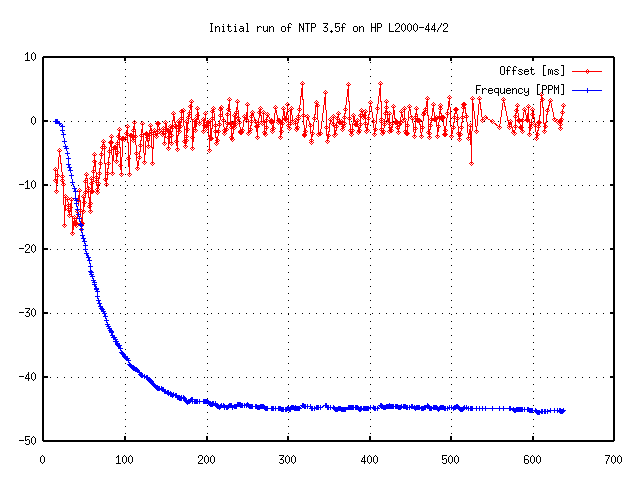
\includegraphics[height=8cm]{images/ntp-graph.png}
        \scriptsize\url{http://www.ntp.org/ntpfaq/NTP-s-algo.htm}
    \end{center}
\end{frame}
\inlineslide{s:ntp-graph}{}\label{l:ntp-graph}

The fact that clocks may be stepped by NTP, i.e.\ suddenly moved forwards or backwards, has an important implication for any software that needs to measure elapsed time.
\autoref{l:monotonic-clock} shows an example in Java, in which we want to measure the running time of a function \verb|doSomething()|.
Java has two core functions for getting the current timestamp from the operating system's local clock: \verb|currentTimeMillis()| and \verb|nanoTime()|.
Besides the different resolution (milliseconds versus nanoseconds), the key difference between the two is how they behave in the face of clock adjustments from NTP or other sources.

\verb|currentTimeMillis()| is a \emph{time-of-day} clock (also known as \emph{real-time} clock) that returns the time elapsed since a fixed reference point (in this case, the Unix epoch of 1 January 1970).
When the NTP client steps the local clock, a time-of-day clock may jump.
Thus, if you use such a clock to measure elapsed time, the resulting difference between end timestamp and start timestamp may be much greater than the actual elapsed time (if the clock was stepped forwards), or it may even be negative (if the clock was stepped backwards).
This type of clock is therefore not suitable for measuring elapsed time.

On the other hand, \verb|nanoTime()| is a \emph{monotonic} clock, which is not affected by NTP stepping: it still counts seconds elapsed, but it always moves forward.
Only the rate at which it moves forward may be adjusted by NTP slewing.
This makes a monotonic clock much more robust for measuring elapsed time.
The downside is that a timestamp from a monotonic clock is meaningless by itself: it measures the time since some arbitrary reference point, such as the time since this computer was started up.
When using a monotonic clock, only the difference between two timestamps from the same node is meaningful.
It does not make sense to compare monotonic clock timestamps across different nodes.

\begin{frame}
    \label{s:monotonic-clock}
    \frametitle{Monotonic and time-of-day clocks}
    \inputminted{java}{code/nonmonotonic.java}
    \begin{tikzpicture}[remember picture,overlay]
        \node (dosomething) [xshift=-2.2cm,yshift=1.8cm] at (current page.center) {};
        \node<2-> (stepping) [xshift=2.5cm,yshift=-0.5cm,red] at (current page.center) {NTP client steps the clock during this};
        \draw<2-> [-Stealth,red,line width=4pt] (stepping) .. controls +(0,2) and +(2,0) .. (dosomething);
    \end{tikzpicture}
    \uncover<3->{\inputminted{java}{code/monotonic.java}}
\end{frame}
\inlineslide{s:monotonic-clock}{}\label{l:monotonic-clock}

Most operating systems and programming languages provide both a time-of-day clock and a monotonic clock, since both are useful for different purposes.

\begin{frame}
    \label{s:monotonic-comparison}
    \frametitle{Monotonic and time-of-day clocks}
    \textbf{Time-of-day clock:}
    \begin{itemize}
        \item<1-> Time since a fixed date (e.g.\ 1 January 1970 epoch)
        \item<2-> May suddenly move forwards or backwards (NTP stepping), subject to leap second adjustments
        \item<3-> Timestamps can be compared across nodes (if synced)
        \item<4-> Java: \texttt{System.currentTimeMillis()}
        \item<4-> Linux: \texttt{clock\char`_gettime(CLOCK\char`_REALTIME)}\\[1em]
    \end{itemize}
    \textbf{Monotonic clock:}
    \begin{itemize}
        \item<1-> Time since arbitrary point (e.g.\ when machine booted up)
        \item<2-> Always moves forwards at near-constant rate
        \item<3-> Good for measuring elapsed time on a single node
        \item<4-> Java: \texttt{System.nanoTime()}
        \item<4-> Linux: \texttt{clock\char`_gettime(CLOCK\char`_MONOTONIC)}
    \end{itemize}
\end{frame}
\inlineslide{s:monotonic-comparison}{}\label{l:monotonic-comparison}

\subsection{Causality and happens-before}\label{sec:causality}

We will now move on to the problem of ordering events in a distributed system, which is closely related to the concept of time.
Consider the scenario on \autoref{l:moon-cheese}, in which user A makes a statement $m_1$ and sends it as a message to the other two users, B and C.
On receiving $m_1$, user B reacts by sending a reply $m_2$ to the other two users, A and C.
However, even if we assume the network links are reliable, they allow reordering (\autoref{l:model-network}), so C might receive $m_2$ before $m_1$ if $m_1$ is slightly delayed in the network.

From C's point of view, the result is confusing: C first sees the reply, and then the message it is replying to.
It almost looks as though B was able to see into the future and anticipate A's statement before A even said it.
In real life this sort of reordering of spoken words does not happen, and so we intuitively don't expect it to happen in computer systems either.

As a more technical example, consider $m_1$ to be an instruction that creates an object in a database, and $m_2$ to be an instruction that updates this same object.
If a node processes $m_2$ before $m_1$ it would first attempt to update a nonexistent object, and then create an object which would not subsequently be updated.
The database instructions only make sense if $m_1$ is processed before $m_2$.

\begin{frame}
    \label{s:moon-cheese}
    \frametitle{Ordering of messages}
    \begin{center}
        \begin{tikzpicture}
            \node [rectangle,fill=red!10,draw] (user1) at (0,3.7) {user A};
            \node [rectangle,fill=red!10,draw] (user2) at (4,3.7) {user B};
            \node [rectangle,fill=red!10,draw] (user3) at (8,3.7) {user C};
            \draw (user1) -- (0,0.2);
            \draw (user2) -- (4,0.2);
            \draw (user3) -- (8,0.2);
            \draw<1-> [bigarrow] (0,3.0)
                .. node [above,sloped] {$m_1$} controls (2,2.75) .. (4,2.5)
                .. controls (5,2.375) and (5,0.875) .. (6,0.75) -- (8,0.5);
            \draw<1-> [bigarrow] (0,2.9)
                .. controls (1,2.775) and (1,2.3) .. (2,2.05)
                -- node [above,sloped] {$m_1$} (4,1.8);
            \draw<2-> [bigarrow] (4,1.5) -- node [above,sloped] {$m_2$} (8,1.0);
            \draw<2-> [bigarrow] (4,1.4) -- node [above,sloped] {$m_2$} (0,0.9);
        \end{tikzpicture}
    \end{center}
    \uncover<1->{$m_1 = $ ``A says: The moon is made of cheese!''}\\
    \uncover<2->{$m_2 = $ ``B says: Oh no it isn't!''}\\[1em]%
    \uncover<3->{C sees $m_2$ first, $m_1$ second,\\even though logically $m_1$ \textbf{happened before} $m_2$.}
\end{frame}
\inlineslide{s:moon-cheese}{}\label{l:moon-cheese}

How can C determine the correct order in which it should put the messages?
A monotonic clock won't work since its timestamps are not comparable across nodes.
A first attempt might be to get a timestamp from a time-of-day clock whenever a user wants to send a message, and to attach that timestamp to the message.
In this scenario, we might reasonably expect $m_2$ to have a later timestamp than $m_1$, since $m_2$ is a response to $m_1$ and so $m_2$ must have happened after $m_1$.

Unfortunately, in a partially synchronous system model, this does not work reliably.
The clock synchronisation performed by NTP and similar protocols always leaves some residual uncertainty about the exact skew between two clocks, especially if the network latency in the two directions is asymmetric.
We therefore cannot rule out the following scenario: A sends $m_1$ with timestamp $t_1$ according to A's clock.
When B receives $m_1$, the timestamp according to B's clock is $t_2$, where $t_2 < t_1$, because A's clock is slightly ahead of B's clock.
Thus, if we order messages based on their timestamps from time-of-day clocks, we might again end up with the wrong order.

\begin{frame}<1-2>[label=physical-order]
    \label{s:physical-order}
    \frametitle<1-2>{Ordering of messages using timestamps?}
    \frametitle<3>{Physical timestamps inconsistent with causality}
    \begin{center}
        \begin{tikzpicture}
            \node [rectangle,fill=red!10,draw] (user1) at (0,3.7) {user A};
            \node [rectangle,fill=red!10,draw] (user2) at (4,3.7) {user B};
            \node [rectangle,fill=red!10,draw] (user3) at (8,3.7) {user C};
            \draw (user1) -- (0,0.2);
            \draw (user2) -- (4,0.2);
            \draw (user3) -- (8,0.2);
            \draw [bigarrow] (0,3.0)
                .. node [above,sloped] {$m_1$} node [at start,left,fill=yellow!50] {$t_1$} controls (2,2.75) .. (4,2.5)
                .. controls (5,2.375) and (5,0.875) .. (6,0.75) -- (8,0.5);
            \draw [bigarrow] (0,2.9)
                .. controls (1,2.775) and (1,2.3) .. (2,2.05)
                -- node [above,sloped] {$m_1$} node [at end,right,fill=yellow!50] {$t_2$} (4,1.8);
            \draw [bigarrow] (4,1.5) -- node [above,sloped] {$m_2$} (8,1.0);
            \draw [bigarrow] (4,1.4) -- node [above,sloped] {$m_2$} (0,0.9);
        \end{tikzpicture}
    \end{center}
    $m_1 = (t_1, \text{``A says: The moon is made of cheese!''})$\\
    $m_2 = (t_2, \text{``B says: Oh no it isn't!''})$\\[1em]%
    \uncover<2->{\textbf{Problem}: even with synced clocks, $t_2 < t_1$ is possible.\\
    Timestamp order is inconsistent with expected order!}
\end{frame}
\inlineslide{s:physical-order}{}\label{l:physical-order}

To formalise what we mean with the ``correct'' order in this type of scenario, we use the \emph{happens-before relation} as defined on \autoref{l:happens-before}.
This definition assumes that each node has only a single thread of execution, so for any two execution steps of a node, it is clear which one happened first.
More formally, we assume that there is a \emph{strict total order} on the events that occur at the same node.
A multithreaded process can be modelled by using a separate node to represent each thread.

We then extend this order across nodes by defining that a message is sent before that same message is received (in other words, we rule out time travel: it is not possible to receive a message that has not yet been sent).
For convenience, we assume that every sent message is unique, so when a message is received, we always know unambiguously where and when that message was sent.
In practice, duplicate messages may exist, but we can make them unique, for example by including the ID of the sender node and a sequence number in each message.

Finally, we take the transitive closure, and the result is the happens-before relation.
This is a \emph{partial order}, which means that it is possible that for some events $a$ and $b$, neither $a$ happened before $b$, nor $b$ happened before $a$.
In that case, we call $a$ and $b$ \emph{concurrent}.
Note that here, ``concurrent'' does not mean literally ``at the same time'', but rather that $a$ and $b$ are independent in the sense that there is no sequence of messages leading from one to the other.

\begin{frame}
    \label{s:happens-before}
    \frametitle{The happens-before relation}
    An \textbf{event} is something happening at one node (sending or receiving a message, or a local execution step).\\[1em]
    We say event $a$ \textbf{happens before} event $b$ (written $a \rightarrow b$) iff:\pause
    \begin{itemize}
        \item $a$ and $b$ occurred at the same node, and $a$ occurred before $b$ in that node's local execution order; or\pause
        \item event $a$ is the sending of some message $m$, and event $b$ is the receipt of that same message $m$ (assuming sent messages are unique); or\pause
        \item there exists an event $c$ such that $a \rightarrow c$ and $c \rightarrow b$.\\[1em]\pause
    \end{itemize}
    The happens-before relation is a partial order:
    it is possible that neither $a \rightarrow b$ nor $b \rightarrow a$.
    In that case, $a$ and $b$ are \textbf{concurrent} (written $a \parallel b$).
\end{frame}
\inlineslide{s:happens-before}{}\label{l:happens-before}

\begin{frame}
    \label{s:hb-example}
    \frametitle{Happens-before relation example}
    \begin{center}
        \begin{tikzpicture}
            \node [rectangle,fill=red!10,draw] (A) at (0,3.7) {A};
            \node [rectangle,fill=red!10,draw] (B) at (4,3.7) {B};
            \node [rectangle,fill=red!10,draw] (C) at (8,3.7) {C};
            \draw (A) -- (0,0.5);
            \draw (B) -- (4,0.5);
            \draw (C) -- (8,0.5);
            \tikzstyle{event}=[circle,fill=black,inner sep=2pt]
            \node (a) [event] at (0,3.0) {}; \draw (a) node [left,xshift=-0.1cm] {$a$};
            \node (b) [event] at (0,2.5) {}; \draw (b) node [left,xshift=-0.1cm] {$b$};
            \node (c) [event] at (4,2.0) {}; \draw (c) node [right,xshift=0.1cm] {$c$};
            \node (d) [event] at (4,1.5) {}; \draw (d) node [left,xshift=-0.1cm] {$d$};
            \node (e) [event] at (8,2.8) {}; \draw (e) node [right,xshift=0.1cm] {$e$};
            \node (f) [event] at (8,1.0) {}; \draw (f) node [right,xshift=0.1cm] {$f$};
            \draw [bigarrow] (b) -- node[above] {$m_1$} (c);
            \draw [bigarrow] (d) -- node[above] {$m_2$} (f);
        \end{tikzpicture}
    \end{center}\pause
    \begin{itemize}
        \item $a \rightarrow b$, $c \rightarrow d$, and $e \rightarrow f$ due to node execution order\pause
        \item $b \rightarrow c$ and $d \rightarrow f$ due to messages $m_1$ and $m_2$\pause
        \item $a \rightarrow c$, $a \rightarrow d$, $a \rightarrow f$, $b \rightarrow d$, $b \rightarrow f$,
            and $c \rightarrow f$ due to transitivity\pause
        \item $a \parallel e$, $b \parallel e$, $c \parallel e$, and $d \parallel e$
    \end{itemize}
\end{frame}
\inlineslide{s:hb-example}{}\label{l:hb-example}

\supervision{\label{q:strict-partial-order}
    A relation $R$ is a \emph{strict partial order} if it is irreflexive ($\nexists a.\; (a,a) \in R$) and transitive ($\forall a,b,c.\; (a,b) \in R \wedge (b,c) \in R \Longrightarrow (a,c) \in R$).
    (These two conditions also imply that it $R$ asymmetric, i.e.\ that $\forall a,b.\; (a,b) \in R \Longrightarrow (b,a) \notin R$.)
    Prove that the happens-before relation is a strict partial order.
    You may assume that any two nodes are a nonzero distance apart, as well as the physical principle that information cannot travel faster than the speed of light.
}{
    The fact that happens-before is transitive follows directly from the third bullet point of its definition.

    To prove that it is irreflexive, we use proof by contradiction.
    Assume to the contrary that there exists $a$ such that $a \rightarrow a$.
    This implies at least one of the following:
    \begin{enumerate}
        \item $a$ occurred before $a$ in some node's local execution order.
            However, this contradicts our assumption that every node's local execution forms a strict total order, which is irreflexive.
        \item $a$ is the sending of some message $m$, and $a$ is the receipt of that same message $m$.
            This is impossible because sending and receiving a message are two different events.
        \item There exists an event $b$ such that $a \rightarrow b$ and $b \rightarrow a$.
            Let $N_a$ be the node at which $a$ occurs, and $N_b$ the node at which $b$ occurs.
            Then either $N_a = N_b$ or $N_a \neq N_b$.
            If $N_a = N_b$ then $a \rightarrow b$ and $b \rightarrow a$ contradict our assumption that every node's local execution forms a strict total order, so we have $N_a \neq N_b$.

            Let $t_a$ be the time at which $a$ occurs and let $t_b$ be the time at which $b$ occurs, both according to $N_a$'s clock.
            Let $d$ be the distance in space between $N_a$ and $N_b$.
            $a \rightarrow b$ implies the existence of a message, or a sequence of messages (possibly via other nodes), through which information can travel from $a$ to $b$.
            Since this information cannot travel faster than the speed of light, we have $t_b \ge t_a + \frac{d}{c}$, where $c$ is the speed of light.
            By similar argument, $b \rightarrow a$ implies that $t_a \ge t_b + \frac{d}{c}$.

            Since we are assuming $d > 0$ and the speed of light is finite, $\frac{d}{c} > 0$.
            Therefore we have $t_b > t_a$ and $t_a > t_b$, a contradiction.
    \end{enumerate}
}

\supervision{\label{q:hb-three-cases}
    Show that for any two events $a$ and $b$, exactly one of the three following statements must be true: either $a \rightarrow b$, or $b \rightarrow a$, or $a \parallel b$.
}{
    The statement $a \rightarrow b$ must be either true or false.
    If it is true, then it is not the case that $a \parallel b$ by definition.
    Moreover, since the happens-before relation is a strict partial order (\autoref{q:strict-partial-order}), $a \rightarrow b$ implies $b \not\rightarrow a$.

    If $a \not\rightarrow b$, consider the statement $b \rightarrow a$, which must be either true or false.
    If it is true, then it is not the case that $a \parallel b$ by definition.
    If it is false, then $a \parallel b$ by definition.

    In all cases examined, exactly one of the three statements $\{a \rightarrow b,\; b \rightarrow a,\; a \parallel b\}$ is true.
}

The happens-before relation is a way of reasoning about \emph{causality} in distributed systems.
Causality considers whether information could have flowed from one event to another, and thus whether one event may have influenced another.
In the example of \autoref{l:moon-cheese}, $m_2$ (``Oh no it isn't!'') is a reply to $m_1$ (``The moon is made of cheese!''), and so $m_1$ influenced $m_2$.
Whether one event truly ``caused'' another is a philosophical question that we don't need to answer now; what matters for our purposes is that the sender of $m_2$ had already received $m_1$ at the time of sending $m_2$.

\begin{frame}
    \label{s:causality}
    \frametitle{Causality}
    Taken from physics (relativity).
    \begin{itemize}
        \item When $a \rightarrow b$, then $a$ \textbf{might have caused} $b$.
        \item When $a \parallel b$, we know that $a$ \textbf{cannot have caused} $b$.
    \end{itemize}
    Happens-before relation encodes \textbf{potential causality}.\pause
    \begin{center}
        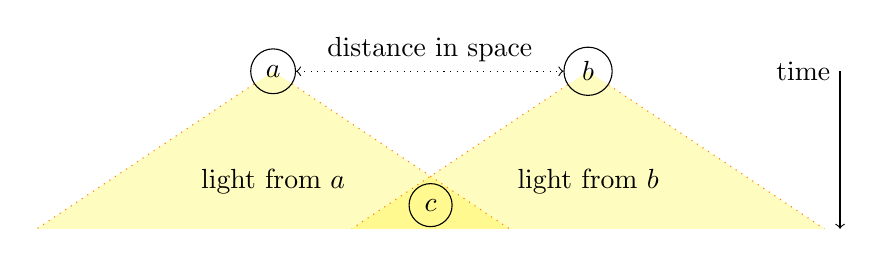
\begin{tikzpicture}
            \fill<3-> [yellow,nearly transparent] (0,2) -- (3,0) -- (-3,0) -- cycle;
            \fill<4-> [yellow,nearly transparent] (4,2) -- (7,0) -- (1,0) -- cycle;
            \node<2-> (a) [circle,draw] at (0,2) {$a$};
            \node<2-> (b) [circle,draw] at (4,2) {$b$};
            \node<5-> (c) [circle,draw] at (2,0.3) {$c$};
            \draw<2-> [<->,dotted] (a) -- node [above] {distance in space} (b);
            \draw<3-> [orange,dotted] (a) -- (-3,0);
            \draw<3-> [orange,dotted] (a) -- (3,0);
            \draw<4-> [orange,dotted] (b) -- (1,0);
            \draw<4-> [orange,dotted] (b) -- (7,0);
            \node<3-> at (0,0.6) {light from $a$};
            \node<4-> at (4,0.6) {light from $b$};
            \draw<2-> [->] (7.2,2) -- node [at start,left] {time} (7.2,0);
            \node at (-3,0) {}; \node at (7.2,2.2) {}; % placeholder so that slide 1 doesn't jump
        \end{tikzpicture}
    \end{center}
    \uncover<6->{Let $\prec$ be a strict total order on events.\\
    If $(a \rightarrow b) \Longrightarrow (a \prec b)$ then $\prec$ is a \textbf{causal order}\\
    (or: $\prec$ is ``consistent with causality'').\\
    \textbf{NB.} ``causal'' $\neq$ ``casual''!}
\end{frame}
\inlineslide{s:causality}{}\label{l:causality}

% The above introduction of "consistent with causality" is quite abstract. Introduce it with an example?
% Say the physical timestamp comparison is a total order, happens-before is a partial order

The notion of causality is borrowed from physics, where it is generally believed that it is not possible for information to travel faster than the speed of light.
Thus, if you have two events $a$ and $b$ that occur sufficiently far apart in space, but close together in time, then it is impossible for a signal sent from $a$ to arrive at $b$'s location before event $b$, and vice versa.
Therefore, $a$ and $b$ must be \emph{causally unrelated}.

An event $c$ that is sufficiently close in space to $a$, and sufficiently long after $a$ in time, will be within $a$'s \emph{light cone}: that is, it is possible for a signal from $a$ to reach $c$, and therefore $a$ might influence $c$.
In distributed systems, we usually work with messages on a network rather than beams of light, but the principle is very similar.

% "causality is reachability in spacetime"
% https://twitter.com/palvaro/status/1233208997257170944


\subsection{Logical time}\label{sec:logical-time}

\begin{frame}
    \begin{center}
        {\Large{\color{darkblue}{Broadcast protocols and logical time}}} \\[2em]
        \mydetails
    \end{center}
\end{frame}

\againframe<3>{physical-order}

\begin{frame}
    \label{s:logical-clocks}
    \frametitle{Logical vs. physical clocks}
    \begin{itemize}
        \item Physical clock: count number of \textbf{seconds elapsed}
        \item Logical clock: count number of \textbf{events occurred}\\[1em]
    \end{itemize}
    Physical timestamps: useful for many things, but may be \textbf{inconsistent with causality}.\\[1em]\pause
    Logical clocks: designed to \textbf{capture causal dependencies}.
    \[ (e_1 \rightarrow e_2) \Longrightarrow (T(e_1) < T(e_2)) \]\pause
    We will look at two types of logical clocks:
    \begin{itemize}
        \item Lamport clocks
        \item Vector clocks
    \end{itemize}
\end{frame}
\inlineslide{s:logical-clocks}{}\label{l:logical-clocks}

Recall that on \autoref{l:physical-order}, we saw that timestamps from physical clocks can be inconsistent with causality, even if those clocks are synchronised using something like NTP.
That is, if $\mathsf{send}(m)$ is the event of sending message $m$, and if the happens-before relation indicates that $\mathsf{send}(m_1) \rightarrow \mathsf{send}(m_2)$, then it could nevertheless happen that the the physical timestamp of $\mathsf{send}(m_1)$ (according to the clock of $m_1$'s sender) is less than the physical timestamp of $\mathsf{send}(m_2)$ (according to the clock of $m_2$'s sender).

In contrast, \emph{logical clocks} focus on correctly capturing the order of events in a distributed system.
The first type of logical clock we will examine is the Lamport clock, introduced by \citet{Lamport:1978} in one of the seminal papers of distributed computing.

\begin{frame}
    \label{s:lamport-definition}
    \frametitle{Lamport clocks algorithm}
    \begin{algorithmic}
        \On{initialisation}
            \State $t := 0$ \Comment{each node has its own local variable $t$}
        \EndOn
        \State
        \On{any event occurring at the local node}
            \State $t := t + 1$
        \EndOn
        \State
        \On{request to send message $m$}
            \State $t := t + 1$; send $(t, m)$ via the underlying network link
        \EndOn
        \State
        \On{receiving $(t', m)$ via the underlying network link}
            \State $t := \mathrm{max}(t, t') + 1$
            \State deliver $m$ to the application
        \EndOn
    \end{algorithmic}
\end{frame}
\inlineslide{s:lamport-definition}{}\label{l:lamport-definition}

\begin{frame}
    \label{s:lamport-description}
    \frametitle{Lamport clocks in words}
    \begin{itemize}
        \item Each node maintains a counter $t$,\\incremented on every local event $e$
        \item Let $L(e)$ be the value of $t$ after that increment
        \item Attach current $t$ to messages sent over network
        \item Recipient moves its clock forward to timestamp in the message (if greater than local counter), then increments\\[1em]
    \end{itemize}\pause
    Properties of this scheme:
    \begin{itemize}
        \item If $a \rightarrow b$ then $L(a) < L(b)$\pause
        \item However, $L(a) < L(b)$ does not imply $a \rightarrow b$\pause
        \item Possible that $L(a) = L(b)$ for $a \neq b$
    \end{itemize}
\end{frame}
\inlineslide{s:lamport-description}{}\label{l:lamport-description}

A Lamport timestamp is essentially an integer that counts the number of events that have occurred.
As such, it has no direct relationship to physical time.
On each node, time increases because the integer is incremented on every event.
The algorithm assumes a crash-stop model (or a crash-recovery model if the timestamp is maintained in stable storage, i.e.\ on disk).

When a message is sent over the network, the sender attaches its current Lamport timestamp to that message.
In the example on \autoref{l:lamport-example}, $t=2$ is attached to $m_1$ and $t=4$ is attached to $m_2$.
When the recipient receives a message, it moves its local Lamport clock forward to the timestamp in the message plus one; if the recipient's clock is already ahead of the timestamp in the message, it is only incremented.

Lamport timestamps have the property that if $a$ happened before $b$, then $b$ always has a greater timestamp than $a$; in other words, the timestamps are consistent with causality.
However, the converse is not true: in general, if $b$ has a greater timestamp than $a$, we know that $b \not\rightarrow a$, but we do not know whether $a \rightarrow b$ or $a \parallel b$.

It is also possible for two different events to have the same timestamp.
In the example on \autoref{l:lamport-example}, the third event on node $A$ and the first event on node $B$ both have a timestamp of 3.
If we need a unique timestamp for every event, each timestamp can be extended with the name or identifier of the node on which that event occurred.
Within the scope of a single node, each event is assigned a unique timestamp; thus, assuming each node has a unique name, the combination of timestamp and node name is globally unique (across all nodes).

\begin{frame}
    \label{s:lamport-example}
    \frametitle{Lamport clocks example}
    \begin{center}
        \begin{tikzpicture}
            \node [rectangle,fill=red!10,draw] (A) at (0,3.7) {A};
            \node [rectangle,fill=red!10,draw] (B) at (4,3.7) {B};
            \node [rectangle,fill=red!10,draw] (C) at (8,3.7) {C};
            \draw (A) -- (0,0.5);
            \draw (B) -- (4,0.5);
            \draw (C) -- (8,0.5);
            \tikzstyle{event}=[circle,fill=black,inner sep=2pt]
            \node (a) [event] at (0,3.0) {};
            \node (b) [event] at (0,2.5) {};
            \node (c) [event] at (4,2.0) {};
            \node (d) [event] at (4,1.5) {};
            \node (e) [event] at (8,2.8) {};
            \node (f) [event] at (8,1.0) {};
            \node (g) [event] at (0,1.5) {};
            \draw<1-2| handout:0> (a) node [left,xshift=-0.1cm] {1};
            \draw<1-2| handout:0> (b) node [left,xshift=-0.1cm] {2};
            \draw<1-2| handout:0> (c) node [right,xshift=0.1cm] {3};
            \draw<1-2| handout:0> (d) node [left,xshift=-0.1cm] {4};
            \draw<1-2| handout:0> (e) node [right,xshift=0.1cm] {1};
            \draw<1-2| handout:0> (f) node [right,xshift=0.1cm] {5};
            \draw<1-2| handout:0> (g) node [left,xshift=-0.1cm] {3};
            \draw<3-> (a) node [left,xshift=-0.1cm] {$(1, A)$};
            \draw<3-> (b) node [left,xshift=-0.1cm] {$(2, A)$};
            \draw<3-> (c) node [right,xshift=0.1cm] {$(3, B)$};
            \draw<3-> (d) node [left,xshift=-0.1cm] {$(4, B)$};
            \draw<3-> (e) node [right,xshift=0.1cm] {$(1, C)$};
            \draw<3-> (f) node [right,xshift=0.1cm] {$(5, C)$};
            \draw<3-> (g) node [left,xshift=-0.1cm] {$(3, A)$};
            \draw [bigarrow] (b) -- node[above] {$(2, m_1)$} (c);
            \draw [bigarrow] (d) -- node[below] {$(4, m_2)$} (f);
        \end{tikzpicture}
    \end{center}%
    \uncover<2->{Let $N(e)$ be the node at which event $e$ occurred.\\
    Then the pair $(L(e), N(e))$ \textbf{uniquely identifies} event $e$.}\\[1em]%
    \uncover<4->{Define a \textbf{total order} $\prec$ using Lamport timestamps:
    \[ (a \prec b) \Longleftrightarrow (L(a) < L(b) \;\vee\; (L(a) = L(b) \;\wedge\; N(a) < N(b))) \]
    This order is \textbf{causal}: $(a \rightarrow b) \Longrightarrow (a \prec b)$}
\end{frame}
\inlineslide{s:lamport-example}{}\label{l:lamport-example}

Recall that the happens-before relation is a partial order (\autoref{l:happens-before}).
Using Lamport timestamps we can extend this partial order into a \emph{total order}.
We use the lexicographic order over (timestamp, node name) pairs: that is, we first compare the timestamps, and if they are the same, we break ties by comparing the node names.

This relation $\prec$ puts all events into a linear order: for any two events $a \neq b$ we have either $a \prec b$ or $b \prec a$.
It is a causal order: that is, whenever $a \rightarrow b$ we have $a \prec b$.
In other words, $\prec$ is a \emph{linear extension} of the partial order $\rightarrow$.
However, if $a \parallel b$ we could have either $a \prec b$ or $b \prec a$, so the order of the two events is determined arbitrarily by the algorithm.

\supervision{\label{q:lamport-example}
    Given the sequence of messages in the following execution, show the Lamport timestamps at each send or receive event.

    \begin{center}
    \begin{tikzpicture}
        \node [rectangle,fill=red!10,draw] (A) at (0,7) {A};
        \node [rectangle,fill=red!10,draw] (B) at (3,7) {B};
        \node [rectangle,fill=red!10,draw] (C) at (6,7) {C};
        \node [rectangle,fill=red!10,draw] (D) at (9,7) {D};
        \draw (A) -- (0,0.7);
        \draw (B) -- (3,0.7);
        \draw (C) -- (6,0.7);
        \draw (D) -- (9,0.7);
        \tikzstyle{event}=[circle,fill=black,inner sep=2pt]
        \node (s1) [event] at (0,6.5) {};
        \node (r1) [event] at (3,6.2) {};
        \node (s2) [event] at (0,6.0) {};
        \node (r2) [event] at (6,5.4) {};
        \node (s3) [event] at (0,5.5) {};
        \node (r3) [event] at (9,4.6) {};
        \node (s4) [event] at (3,4.7) {};
        \node (r4) [event] at (9,4.1) {};
        \node (s5) [event] at (3,4.2) {};
        \node (r5) [event] at (6,3.9) {};
        \node (s6) [event] at (6,3.4) {};
        \node (r6) [event] at (9,3.1) {};
        \node (s7) [event] at (6,2.9) {};
        \node (r7) [event] at (0,2.3) {};
        \node (s8) [event] at (0,1.8) {};
        \node (r8) [event] at (3,1.5) {};
        \node (s9) [event] at (6,1.3) {};
        \node (r9) [event] at (3,1.0) {};
        \draw [bigarrow] (s1) -- node[above] {$m_1$} (r1);
        \draw [bigarrow] (s2) -- node[above,pos=0.25] {$m_2$} (r2);
        \draw [bigarrow] (s3) -- node[above,pos=0.17] {$m_3$} (r3);
        \draw [bigarrow] (s4) -- node[above,pos=0.25] {$m_4$} (r4);
        \draw [bigarrow] (s5) -- node[above] {$m_5$} (r5);
        \draw [bigarrow] (s6) -- node[above] {$m_6$} (r6);
        \draw [bigarrow] (s7) -- node[above,pos=0.25] {$m_7$} (r7);
        \draw [bigarrow] (s8) -- node[above] {$m_8$} (r8);
        \draw [bigarrow] (s9) -- node[above] {$m_9$} (r9);
    \end{tikzpicture}
    \end{center}
}{
    The following table shows both the Lamport timestamps from this exercise and the vector timestamps from \autoref{q:vector-example}.

    % Based on Steven Hand & Robert Watson's problem sheet
    \begin{center}
    \begin{tabular}{|c|cccc|cccc|}
    \hline
    Message & \multicolumn{4}{c|}{Lamport} & \multicolumn{4}{c|}{Vector} \\
            &  A &  B &  C &  D            & A & B & C & D \\
    \hline
    initial &  0 & 0  &  0 &  0            & $\langle 0, 0, 0, 0 \rangle$
                                           & $\langle 0, 0, 0, 0 \rangle$
                                           & $\langle 0, 0, 0, 0 \rangle$
                                           & $\langle 0, 0, 0, 0 \rangle$ \\
    \hline
    $m_1$   &  1 &  2 & -- & --            & $\langle 1, 0, 0, 0 \rangle$
                                           & $\langle 1, 1, 0, 0 \rangle$
                                           & --
                                           & -- \\
    $m_2$   &  2 & -- &  3 & --            & $\langle 2, 0, 0, 0 \rangle$
                                           & --
                                           & $\langle 2, 0, 1, 0 \rangle$
                                           & -- \\
    $m_3$   &  3 & -- & -- &  4            & $\langle 3, 0, 0, 0 \rangle$
                                           & --
                                           & --
                                           & $\langle 3, 0, 0, 1 \rangle$ \\
    $m_4$   & -- &  3 & -- &  5            & --
                                           & $\langle 1, 2, 0, 0 \rangle$
                                           & --
                                           & $\langle 3, 2, 0, 2 \rangle$ \\
    $m_5$   & -- &  4 &  5 & --            & --
                                           & $\langle 1, 3, 0, 0 \rangle$
                                           & $\langle 2, 3, 2, 0 \rangle$
                                           & -- \\
    $m_6$   & -- & -- &  6 &  7            & --
                                           & --
                                           & $\langle 2, 3, 3, 0 \rangle$
                                           & $\langle 3, 3, 3, 3 \rangle$ \\
    $m_7$   &  8 & -- &  7 & --            & $\langle 4, 3, 4, 0 \rangle$
                                           & --
                                           & $\langle 2, 3, 4, 0 \rangle$
                                           & -- \\
    $m_8$   &  9 & 10 & -- & --            & $\langle 5, 3, 4, 0 \rangle$
                                           & $\langle 5, 4, 4, 0 \rangle$
                                           & --
                                           & -- \\
    $m_9$   & -- & 11 &  8 & --            & --
                                           & $\langle 5, 5, 5, 0 \rangle$
                                           & $\langle 2, 3, 5, 0 \rangle$
                                           & -- \\
    \hline
    final   &  9 & 11 &  8 & 7             & $\langle 5, 3, 4, 0 \rangle$
                                           & $\langle 5, 5, 5, 0 \rangle$
                                           & $\langle 2, 3, 5, 0 \rangle$
                                           & $\langle 3, 3, 3, 3 \rangle$ \\
    \hline
    \end{tabular}
    \end{center}
}

\supervision{
    Prove that the total order $\prec$ using Lamport timestamps is a causal order.
}{
    We assume $a \rightarrow b$ for some events $a$ and $b$.
    Because the happens-before relation is a strict partial order (\autoref{q:strict-partial-order}) we have $a \neq b$.
    To show that $a \prec b$ we use induction over the recursive structure of the definition of the happens-before relation.
    That is, we consider three cases:
    \begin{enumerate}
        \item First base case: $a \rightarrow b$ because $a$ and $b$ occurred at the same node, and $a$ occurred before $b$ in that node's local execution order.
            Then $L(a) < L(b)$ because the algorithm for Lamport timestamps only ever increases a node's local clock, and every local event increases the clock, so an event that occurs later in a node's local execution must have a greater timestamp.
            Hence $a \prec b$.
        \item Second base case: $a \rightarrow b$ because $a = \mathsf{send}(m)$ and $b = \mathsf{receive}(m)$ for some message $m$.
            Then $L(a)$ is included in the message $m$, and so $L(b) = \mathrm{max}(t, L(a)) + 1 > L(a)$ by the definition of the Lamport timestamp algorithm.
            Therefore $L(a) < L(b)$ and hence $a \prec b$.
        \item Inductive step: $a \rightarrow b$ because there exists an event $c$ such that $a \rightarrow c$ and $c \rightarrow b$.
            Then $a \prec c$ and $c \prec b$ by the inductive hypothesis.
            Since $\prec$ is a total order, it is transitive, and therefore $a \prec b$.
    \end{enumerate}
}

Given the Lamport timestamps of two events, it is in general not possible to tell whether those events are concurrent or whether one happened before the other.
If we do want to detect when events are concurrent, we need a different type of logical time: a \emph{vector clock}.

While Lamport timestamps are just a single integer (possibly with a node name attached), vector timestamps are a list of integers, one for each node in the system.
By convention, if we put the $n$ nodes into a vector $\langle N_0, N_1, \dots, N_{n-1} \rangle$, then a vector timestamp is a similar vector $\langle t_0, t_1, \dots, t_{n-1} \rangle$ where $t_i$ is the entry corresponding to node $N_i$.
The value of $t_i$ is the number of events known to have occurred at node $N_i$.
In a vector $T = \langle t_0, t_1, \dots, t_{n-1} \rangle$ we refer to element $t_i$ as $T[i]$, like an index into an array.

\begin{frame}
    \label{s:vector-clocks}
    \frametitle{Vector clocks}
    Given Lamport timestamps $L(a)$ and $L(b)$ with $L(a) < L(b)$\\we can't tell whether $a \rightarrow b$ or $a \parallel b$.\\[1em]
    If we want to detect which events are concurrent, we need \textbf{vector clocks}:\pause
    \begin{itemize}
        \item Assume $n$ nodes in the system, $N = \langle N_0, N_1, \dots, N_{n-1} \rangle$\pause
        \item Vector timestamp of event $a$ is $V(a) = \langle t_0, t_1, \dots, t_{n-1}\rangle$
        \item $t_i$ is number of events observed by node $N_i$\pause
        \item Each node has a current vector timestamp $T$
        \item On event at node $N_i$, increment vector element $T[i]$\pause
        \item Attach current vector timestamp to each message
        \item Recipient merges message vector into its local vector
    \end{itemize}
\end{frame}
\inlineslide{s:vector-clocks}{}\label{l:vector-clocks}

Apart from the difference between a scalar and a vector, the vector clock algorithm is very similar to a Lamport clock (compare \autoref{l:lamport-definition} and \autoref{l:vector-definition}).
A node initialises its vector clock to contain a zero for each node in the system.
Whenever an event occurs at node $N_i$, it increments the $i$th entry (its own entry) in its vector clock.
(In practice, this vector is often implemented as a map from node IDs to integers rather than an array of integers.)
When a message is sent over the network, the sender's current vector timestamp is attached to the message.
Finally, when a message is received, the recipient merges the vector timestamp in the message with its local timestamp by taking the element-wise maximum of the two vectors, and then the recipient increments its own entry.

\begin{frame}
    \label{s:vector-definition}
    \frametitle{Vector clocks algorithm}
    \begin{algorithmic}
        \On{initialisation at node $N_i$}
            \State $T := \langle 0, 0, \dots, 0 \rangle$ \Comment{local variable at node $N_i$}
        \EndOn
        \State
        \On{any event occurring at node $N_i$}
            \State $T[i] := T[i] + 1$
        \EndOn
        \State
        \On{request to send message $m$ at node $N_i$}
            \State $T[i] := T[i] + 1$; send $(T, m)$ via network
        \EndOn
        \State
        \On{receiving $(T', m)$ at node $N_i$ via the network}
            \State $T[j] := \mathrm{max}(T[j], T'[j])$ for every $j \in \{1, \dots, n\}$
            \State $T[i] := T[i] + 1$; deliver $m$ to the application
        \EndOn
    \end{algorithmic}
\end{frame}
\inlineslide{s:vector-definition}{}\label{l:vector-definition}

\autoref{l:vector-example} shows an example of this algorithm in action.
Note that when $C$ receives message $m_2$ from $B$, the vector entry for $A$ is also updated to 2 because this event has an indirect causal dependency on the two events that happened at $A$.
In this way, the vector timestamps mirror the transitivity of the happens-before relation.

\begin{frame}
    \label{s:vector-example}
    \frametitle{Vector clocks example}
    Assuming the vector of nodes is $N = \langle A, B, C \rangle$:
    \begin{center}
        \begin{tikzpicture}
            \node [rectangle,fill=red!10,draw] (A) at (0,3.7) {A};
            \node [rectangle,fill=red!10,draw] (B) at (4,3.7) {B};
            \node [rectangle,fill=red!10,draw] (C) at (8,3.7) {C};
            \draw (A) -- (0,0.5);
            \draw (B) -- (4,0.5);
            \draw (C) -- (8,0.5);
            \tikzstyle{event}=[circle,fill=black,inner sep=2pt]
            \node (a) [event] at (0,3.0) {};
            \node (b) [event] at (0,2.5) {};
            \node (c) [event] at (4,2.0) {};
            \node (d) [event] at (4,1.5) {};
            \node (e) [event] at (8,2.8) {};
            \node (f) [event] at (8,1.0) {};
            \node (g) [event] at (0,1.5) {};
            \draw (a) node [left,xshift=-0.1cm] {$\langle 1, 0, 0 \rangle$};
            \draw (b) node [left,xshift=-0.1cm] {$\langle 2, 0, 0 \rangle$};
            \draw (c) node [right,xshift=0.1cm] {$\langle 2, 1, 0 \rangle$};
            \draw (d) node [left,xshift=-0.1cm] {$\langle 2, 2, 0 \rangle$};
            \draw (e) node [right,xshift=0.1cm] {$\langle 0, 0, 1 \rangle$};
            \draw (f) node [right,xshift=0.1cm] {$\langle 2, 2, 2 \rangle$};
            \draw (g) node [left,xshift=-0.1cm] {$\langle 3, 0, 0 \rangle$};
            \draw [bigarrow] (b) -- node[above,sloped] {$(\langle 2, 0, 0 \rangle, m_1)$} (c);
            \draw [bigarrow] (d) -- node[below,sloped] {$(\langle 2, 2, 0 \rangle, m_2)$} (f);
        \end{tikzpicture}
    \end{center}\pause
    The vector timestamp of an event $e$ represents a set of events, $e$ and its causal dependencies:
    $ \{e\} \cup \{a \mid a \rightarrow e\} $\\[1em]
    For example, $\langle 2, 2, 0\rangle$ represents the first two events from A, the first two events from B, and no events from C.
\end{frame}
\inlineslide{s:vector-example}{}\label{l:vector-example}

\begin{frame}[label=vector-ordering]
    \label{s:vector-ordering}
    \frametitle{Vector clocks ordering}
    Define the following order on vector timestamps\\(in a system with $n$ nodes):
    \begin{itemize}
        \item $T = T'$ iff $T[i] = T'[i]$ for all $i \in \{0, \dots, n-1\}$
        \item $T \le T'$ iff $T[i] \le T'[i]$ for all $i \in \{0, \dots, n-1\}$
        \item $T < T'$ iff $T \le T'$ and $T \ne T'$
        \item $T \parallel T'$ iff $T \not\le T'$ and $T' \not\le T$\\[1em]
    \end{itemize}\pause
    $V(a) \le V(b)$ iff $(\{a\} \cup \{e \mid e \rightarrow a\}) \subseteq (\{b\} \cup \{e \mid e \rightarrow b\})$\\[1em]\pause
    Properties of this order:
    \begin{itemize}
        \item $(V(a) < V(b)) \Longleftrightarrow (a \rightarrow b)$
        \item $(V(a) = V(b)) \Longleftrightarrow (a = b)$
        \item $(V(a) \parallel V(b)) \Longleftrightarrow (a \parallel b)$
    \end{itemize}
\end{frame}
\inlineslide{s:vector-ordering}{}\label{l:vector-ordering}

We then define a partial order over vector timestamps as shown on \autoref{l:vector-ordering}.
We say that one vector is less than or equal to another vector if every element of the first vector is less than or equal to the corresponding element of the second vector.
One vector is strictly less than another vector if they are less than or equal, and if they differ in at least one element.
However, two vectors are incomparable if one vector has a greater value in one element, and the other has a greater value in a different element.
For example, $T = \langle 2, 2, 0\rangle$ and $T' = \langle 0, 0, 1\rangle$ are incomparable because $T[1] > T'[1]$ but $T[3] < T'[3]$.

% TODO: vector representation is not practical in systems where nodes can join and leave; explain alternative representation as map from node ID to integer
% also acknowledge that vectors can get quite large, suggest alternatives (e.g. dotted version vectors, tracking dependencies using unique IDs) -- some discussion already appears later in the context of LWW
% Mention Charron-Bost result?

% Note the system model assumptions of these algorithms?

The partial order over vector timestamps corresponds exactly to the partial order defined by the happens-before relation.
Thus, the vector clock algorithm provides us with a mechanism for computing the happens-before relation in practice.

\supervision{\label{q:vector-example}
    Given the same sequence of messages as in \autoref{q:lamport-example}, show the vector clocks at each send or receive event.
}{
    See solution notes for \autoref{q:lamport-example}.
}

\supervision{\label{q:vector-happens-before}
    Using the Lamport and vector timestamps calculated in \autoref{q:lamport-example} and \ref{q:vector-example}, state whether or not the following events can be determined to have a happens-before relationship.

    \begin{center}
    \begin{tabular}{|c|c|c|c|}
    \hline
    \multicolumn{2}{|c|}{Events}                & Lamport & Vector \\
    \hline
    $\mathsf{send}(m_2)$ & $\mathsf{send}(m_3)$ &         &        \\
    $\mathsf{send}(m_3)$ & $\mathsf{send}(m_5)$ &         &        \\
    $\mathsf{send}(m_5)$ & $\mathsf{send}(m_9)$ &         &        \\
    \hline
    \end{tabular}
    \end{center}
}{
    Note that although Lamport clocks cannot determine \emph{happens-before} between nodes, they actually are sufficient to do so within a single node, as a higher local logical time will always reflect a later event.

    \begin{center}
    \begin{tabular}{|c|c|c|c|}
    \hline
    \multicolumn{2}{|c|}{Events}                & Lamport     & Vector \\
    \hline
    $\mathsf{send}(m_2)$ & $\mathsf{send}(m_3)$ & $2 < 3$     & $\langle 2, 0, 0, 0 \rangle <         \langle 3, 0, 0, 0 \rangle$ \\
    $\mathsf{send}(m_3)$ & $\mathsf{send}(m_5)$ & cannot tell & $\langle 3, 0, 0, 0 \rangle \parallel \langle 1, 3, 0, 0 \rangle$ \\
    $\mathsf{send}(m_5)$ & $\mathsf{send}(m_9)$ & cannot tell & $\langle 1, 3, 0, 0 \rangle <         \langle 2, 3, 5, 0 \rangle$ \\
    \hline
    \end{tabular}
    \end{center}
}

% TODO include this exercise? it's a bit hard though.
%\supervision{
%    Prove that the partial order over vector clocks is equivalent to the happens-before relation when vector clocks are computed according to the algorithm above.
%}{
%    We show that $(V(a) < V(b)) \Longleftrightarrow (a \rightarrow b)$ by proving the implication in both directions.
%
%    First, assume that $V(a) < V(b)$, i.e.\ $\forall i.\; V(a)[i] \le V(b)[i]$ and $\exists i.\; V(a)[i] < V(b)[i]$.
%    To prove that $a \rightarrow b$, note that in the vector clock algorithm, the only time when a node updates a vector entry other than its own %is on receiving a vector timestamp over the network.
%}

% Adapted from Robert Watson and Steven Hand's exercise sheet
\supervision{
    We have seen several types of physical clocks (time-of-day clocks with NTP, monotonic clocks) and logical clocks.
    For each of the following uses of time, explain which type of clock is the most appropriate: process scheduling; I/O; distributed filesystem consistency; cryptographic certificate validity; concurrent database updates.
}{
    \begin{description}
        \item [Process scheduling:]
            If we are talking about the operating system scheduler on a single machine, we only need to measure elapsed time (e.g.\ how many milliseconds a particular thread has been running), so a monotonic clock is the most appropriate.
            However, if we are talking about tasks scheduled to run on a particular date at a particular time (e.g.\ using the Unix service \texttt{cron}), a synchronised time-of-day clock is required.
        \item [I/O:]
            Timeouts and retry timers only need to measure elapsed time, so a monotonic clock is fine.
        \item [Distributed filesystem consistency:]
            When tracking file changes, we need to ensure that changes are consistent with causality, which requires a logical clock.
            Probably a vector clock is most appropriate, because it would allow detecting when two different users concurrently modify the same file.

            However, some software also relies on physical last-modification timestamps in a filesystem: for example, \texttt{make(1)} determines whether a file needs to be recompiled based on whether the source file's last-modification-time is earlier or later than that of the compilation output file.
            If the source file is written on one node but the compilation is performed on another node, this requires modification timestamps to be consistent with causality.
            It is also possible that a source file edit happens concurrently with a compilation, which could only be detected using vector clocks.
            However, last-modification timestamps are conventionally taken from a time-of-day clock, and changing these to be vector clocks would introduce compatibility problems.
        \item [Cryptographic certificate validity:]
            A certificate includes a start date (when it becomes valid) and end date (when it ceases to be valid).
            If a node wants to check whether it is within that period, a synchronised time-of-day clock is required.
        \item [Concurrent database updates:]
            Say two clients concurrently read the same object, modify it, and then write back the modified object to the database.
            The database will want to distinguish this from the situation where first client $A$ reads and writes the object, and then client $B$ reads and writes the object (where the version read by $B$ includes $A$'s changes).
            In the first case, the two updates are concurrent, while in the second case, B's update happened after A's update, so B's update should overwrite A's update.
            Distinguishing these two cases requires vector clocks.

            An alternative approach is that the database does not detect whether updates are concurrent, but simply always lets an update with a greater timestamp overwrite an update with a lesser timestamp.
            In this case, Lamport clocks are best, since they provide a total order that is consistent with causality.
    \end{description}
}

This completes our discussion of logical time.
We have seen two key algorithms: Lamport clocks and vector clocks, one providing a total order and the other capturing the partial order of happens-before.
Various other constructions have been proposed: for example, there are hybrid clocks that combine some of the properties of logical and physical clocks \citep{Kulkarni:2014}.


\section{Broadcast}\label{sec:broadcast}

In this section we will examine \emph{broadcast protocols} (also known as \emph{multicast protocols}), that is, algorithms for delivering one message to multiple recipients.
These are a useful building block for higher-level distributed algorithms, as we will see in \autoref{sec:replication}.
Several different broadcast protocols are used in practice, and their main difference is the \emph{order} in which they deliver messages.
As we saw in the last section, the concept of ordering is closely related to clocks and time.

\subsection{Delivery order}\label{sec:delivery-order}

Many networks provide point-to-point (unicast) messaging, in which a message has one specified recipient.
Broadcast protocols generalise networking such that a message is sent to all nodes in some group.
The group membership may be fixed, or the system may provide a way for nodes to join and leave the group.

Some local-area networks provide multicast or broadcast at the hardware level (for example, \emph{IP multicast}), but communication over the Internet typically only allows unicast.
Moreover, hardware-level multicast is typically provided on a \emph{best-effort} basis, which allows messages to be dropped; making it reliable requires retransmission protocols similar to those we will discuss.

The system model assumptions about node behaviour (\autoref{l:model-nodes}) and synchrony (\autoref{l:model-synchrony}) carry over directly to broadcast groups.

\begin{frame}
    \label{s:broadcast-intro}
    \frametitle{Broadcast protocols}
    Broadcast (multicast) is \textbf{group communication}:
    \begin{itemize}
        \item One node sends message, all nodes in group deliver it\pause
        \item Set of group members may be fixed (static) or dynamic\pause
        \item If one node is faulty, remaining group members carry on\pause
        \item Note: concept is more general than IP multicast\\
            (we build upon point-to-point messaging)\\[1em]\pause
    \end{itemize}
    Build upon system models from earlier lecture:
    \begin{itemize}
        \item Can be \textbf{best-effort} (may drop messages) or \\
            \textbf{reliable} (non-faulty nodes deliver every message,\\
            by retransmitting dropped messages)\pause
        \item Asynchronous/partially synchronous timing model\\
            $\Longrightarrow$ \textbf{no upper bound} on message latency
    \end{itemize}
\end{frame}
\inlineslide{s:broadcast-intro}{}\label{l:broadcast-intro}

Before we go into the details, we should clarify some terminology.
When an application wants to send a message to all nodes in the group, it uses an algorithm to \emph{broadcast} it.
To make this happen, the broadcast algorithm then \emph{sends} some messages to other nodes over point-to-point links, and another node \emph{receives} such a message when it arrives over the point-to-point link.
Finally, the broadcast algorithm may \emph{deliver} the message to the application.
As we shall see shortly, there is sometimes a delay between the time when a message is received and when it is delivered.

\begin{frame}
    \label{s:receive-deliver}
    \frametitle{Receiving versus delivering}
    \begin{tikzpicture}[every node/.style={font=\footnotesize,align=center}]
        \node at (0,4.4) {Node $A$:};
        \node at (6,4.4) {Node $B$:};
        \node [rectangle,draw,text width=4cm] (app1) at (0,3.6) {Application};
        \node [rectangle,draw,text width=4cm] (app2) at (6,3.6) {Application};
        \node [rectangle,draw,text width=4cm] (mid1) at (0,1.8) {Broadcast algorithm\\(middleware)};
        \node [rectangle,draw,text width=4cm] (mid2) at (6,1.8) {Broadcast algorithm\\(middleware)};
        \node [rectangle,draw,text width=10cm] (net) at (3,0) {Network};
        \draw<2-> [bigarrow] (app1)     -- node [left,orange]  {\textbf{broadcast}} (mid1);
        \draw<3-> [bigarrow] (-0.5,1.3) -- node [left,red]     {\textbf{send}}      (-0.5,0.25);
        \draw<3-> [bigarrow] (0.5,0.25) -- node [right,violet] {\textbf{receive}}   (0.5,1.3);
        \draw<3-> [bigarrow] (5.5,1.3)  -- node [left,red]     {\textbf{send}}      (5.5,0.25);
        \draw<3-> [bigarrow] (6.5,0.25) -- node [right,violet] {\textbf{receive}}   (6.5,1.3);
        \draw<4-> [bigarrow] (mid2)     -- node [right,blue]   {\textbf{deliver}}   (app2);
    \end{tikzpicture}\\[1em]%
    \uncover<3->{Assume network provides point-to-point \textbf{\color{red}send}/\textbf{\color{violet}receive}}\\[1em]%
    \uncover<4->{After broadcast algorithm \textbf{\color{violet}receives} message from network,
    it may buffer/queue it before \textbf{\color{blue}delivering} to the application}
\end{frame}
\inlineslide{s:receive-deliver}{}\label{l:receive-deliver}

We will examine three different forms of broadcast.
All of these are \emph{reliable}: every message is eventually delivered to every non-faulty node, with no timing guarantees.
However, they differ in terms of the order in which messages may be delivered at each node.
It turns out that this difference in ordering has very fundamental consequences for the algorithms that implement the broadcast.

\begin{frame}
    \label{s:broadcast-order}
    \frametitle{Forms of reliable broadcast}
    \textbf{FIFO broadcast}:\\
    If $m_1$ and $m_2$ are broadcast by the same node, and $\mathsf{broadcast}(m_1) \rightarrow \mathsf{broadcast}(m_2)$, then $m_1$ must be delivered before $m_2$\\[1em]\pause
    \textbf{Causal broadcast}:\\
    If $\mathsf{broadcast}(m_1) \rightarrow \mathsf{broadcast}(m_2)$ then $m_1$ must be delivered before $m_2$\\[1em]\pause
    \textbf{Total order broadcast}:\\
    If $m_1$ is delivered before $m_2$ on one node, then $m_1$ must be delivered before $m_2$ on all nodes\\[1em]\pause
    \textbf{FIFO-total order broadcast}:\\
    Combination of FIFO broadcast and total order broadcast
\end{frame}
\inlineslide{s:broadcast-order}{}\label{l:broadcast-order}

% TODO: the use of \rightarrow in the definitions above is problematic, because broadcast protocols make a distinction between "receiving" and "delivering" a message; when m1 is received but not delivered before m2 is broadcast, it's unclear whether broadcast(m1) -> broadcast(m2) or not.
% A better definition of causal broadcast might be: if m2 is broadcast by node i, and m1 is broadcast by i or delivered by i before m2 is broadcast, then m1 must be delivered before m2 on all nodes.

\begin{frame}
    \label{s:fifo-broadcast}
    \frametitle{FIFO broadcast}
    \begin{center}
        \begin{tikzpicture}
            \node [rectangle,fill=red!10,draw] (A) at (0,4.7) {A};
            \node [rectangle,fill=red!10,draw] (B) at (4,4.7) {B};
            \node [rectangle,fill=red!10,draw] (C) at (8,4.7) {C};
            \draw (A) -- (0,0);
            \draw (B) -- (4,0);
            \draw (C) -- (8,0);
            % broadcast m1
            \node [inner sep=2pt] (send1) at (0,4) {};
            \path<1-> [->,very thick] (send1) edge [leftloop] node {$m_1$} (send1);
            \draw<1-5| handout: 0> [bigarrow] (0,4.0) -- node [above,near start] {$m_1$} (8,3.2);
            \draw<6-> [bigarrow,darkgreen] (0,4.0)
                .. node [above] {$m_1$} controls (2,3.8) .. (6,3.4)
                .. controls (7,3.3) and (7,1.4) .. (8,1.3);
            \draw<1-> [bigarrow] (0,3.9)
                .. controls (1,3.8) and (1,3.2) .. (2,3.1)
                -- node [above] {$m_1$} (4,2.9);
            % broadcast m2
            \node [inner sep=3pt] (send2) at (4,2.2) {};
            \path<2-> [->,very thick] (send2) edge [rightloop] node [yshift=0.2cm] {$m_2$} (send2);
            \draw<2-> [bigarrow] (4,2.4) -- node [above] {$m_2$} (0,2.0);
            \draw<2-> [bigarrow] (4,2.3) -- node [above] {$m_2$} (8,1.9);
            % broadcast m3
            \node [inner sep=2pt] (send3) at (0,1.5) {};
            \path<3-> [->,very thick] (send3) edge [leftloop] node {$m_3$} (send3);
            \draw<3-> [bigarrow] (0,1.5) -- node [above,near start] {$m_3$} (8,0.7);
            \draw<3-> [bigarrow] (0,1.4)
                .. controls (1,1.3) and (1,0.7) .. (2,0.6)
                -- node [above] {$m_3$} (4,0.4);
        \end{tikzpicture}
    \end{center}%
    \uncover<4->{Messages sent by the same node must be delivered in the order they were sent.\\
    Messages sent by different nodes can be delivered in any order.}\\%
    \uncover<5->{Valid orders: $(m_2, m_1, m_3)$ or $(m_1, m_2, m_3)$ or $(m_1, m_3, m_2)$}
\end{frame}
\inlineslide{s:fifo-broadcast}{}\label{l:fifo-broadcast}

The weakest type of broadcast is called \emph{FIFO broadcast}, which is closely related to FIFO links (see \autoref{q:fifo-links}).
In this model, messages sent by the same node are delivered in the order they were sent.
For example, on \autoref{l:fifo-broadcast}, $m_1$ must be delivered before $m_3$, since they were both sent by $A$.
However, $m_2$ can be delivered at any time before, between, or after $m_1$ and $m_3$.

Another detail about these broadcast protocols: we assume that whenever a node broadcasts a message, it also delivers that message to itself (represented as a loopback arrow on \autoref{l:fifo-broadcast}).
This may seem unnecessary at first~-- after all, a node knows what messages it has itself broadcast!~-- but we will need this for total order broadcast.

The example execution on \autoref{l:fifo-broadcast} is valid FIFO broadcast, but it violates causality: node $C$ delivers $m_2$ before $m_1$, even though $B$ broadcast $m_2$ after delivering $m_1$.
\emph{Causal broadcast} provides a stricter ordering property than FIFO broadcast.
As the name suggests, it ensures that messages are delivered in causal order: that is, if the broadcast of one message happened before the broadcast of another message, then all nodes must deliver those two messages in that order.
If two messages are broadcast concurrently, a node may deliver them in either order.

In the example on \autoref{l:fifo-broadcast}, if node $C$ receives $m_2$ before $m_1$, the broadcast algorithm at $C$ will have to \emph{hold back} (delay or buffer) $m_2$ until after $m_1$ has been delivered, to ensure the messages are delivered in causal order.
In the example on \autoref{l:causal-broadcast}, messages $m_2$ and $m_3$ are broadcast concurrently.
Nodes $A$ and $C$ deliver messages in the order $m_1, m_3, m_2$, while node $B$ delivers them in the order $m_1, m_2, m_3$.
Either of these delivery orders is acceptable, since they are both consistent with causality.

\begin{frame}
    \label{s:causal-broadcast}
    \frametitle{Causal broadcast}
    \begin{center}
        \begin{tikzpicture}
            \node [rectangle,fill=red!10,draw] (A) at (0,4.7) {A};
            \node [rectangle,fill=red!10,draw] (B) at (4,4.7) {B};
            \node [rectangle,fill=red!10,draw] (C) at (8,4.7) {C};
            \draw (A) -- (0,0.4);
            \draw (B) -- (4,0.4);
            \draw (C) -- (8,0.4);
            % broadcast m1
            \node [inner sep=2pt] (send1) at (0,4) {};
            \path<1-> [->,very thick] (send1) edge [leftloop] node {$m_1$} (send1);
            \draw<1-> [bigarrow] (0,4.0) -- node [above,near start] {$m_1$} (8,3.2);
            \draw<1-> [bigarrow] (0,3.9)
                .. controls (1,3.8) and (1,3.2) .. (2,3.1)
                -- node [above] {$m_1$} (4,2.9);
            % broadcast m2
            \node [inner sep=3pt] (send2) at (4,2.2) {};
            \path<2-> [->,very thick] (send2) edge [rightloop] node {} (send2);
            \draw<2-> [bigarrow] (4,2.4) -- node [above,near start] {$m_2$} (0,0.8);
            \draw<2-5> [bigarrow] (4,2.3) -- node [above,near start] {$m_2$} (8,0.6);
            \draw<6-| handout:0> [bigarrow,darkgreen] (4,2.3) -- node [above, near start] {$m_2$} (8,1.9);
            % broadcast m3
            \node [inner sep=2pt] (send3) at (0,2.0) {};
            \path<3-> [->,very thick] (send3) edge [leftloop] node {$m_3$} (send3);
            \draw<3-> [bigarrow] (0,2.0) -- node [above,pos=0.1] {$m_3$} (8,1.2);
            \draw<3-> [bigarrow] (0,1.9)
                .. controls (1,1.8) and (1,1.2) .. (2,1.1)
                -- node [above] {$m_3$} (4,0.9);
        \end{tikzpicture}
    \end{center}%
    \uncover<4->{Causally related messages must be delivered in causal order.\\
    Concurrent messages can be delivered in any order.}\\[0.5em]%
    \uncover<5->{Here: $\mathsf{broadcast}(m_1) \rightarrow \mathsf{broadcast}(m_2)$
    and $\mathsf{broadcast}(m_1) \rightarrow \mathsf{broadcast}(m_3)$\\
    $\Longrightarrow$ valid orders are: $(m_1, m_2, m_3)$ or $(m_1, m_3, m_2)$}
\end{frame}
\inlineslide{s:causal-broadcast}{}\label{l:causal-broadcast}

The third type of broadcast is \emph{total order broadcast}, sometimes also known as \emph{atomic broadcast}.
While FIFO and causal broadcast allow different nodes to deliver messages in different orders, total order broadcast enforces consistency across the nodes, ensuring that all nodes deliver messages in the same order.
The precise delivery order is not defined, as long as it is the same on all nodes.

\autoref{l:total-order1} and \ref{l:total-order2} show two example executions of total order broadcast.
On \autoref{l:total-order1}, all three nodes deliver the messages in the order $m_1, m_2, m_3$, while on \autoref{l:total-order2}, all three nodes deliver the messages in the order of $m_1, m_3, m_2$.
Either of these executions is valid, as long as the nodes agree.

As with causal broadcast, nodes may need to hold back messages, waiting for other messages that need to be delivered first.
For example, node $C$ could receive messages $m_2$ and $m_3$ in either order.
If the algorithm has determined that $m_3$ should be delivered before $m_2$, but if node $C$ receives $m_2$ first, then $C$ will need to hold back $m_2$ until after $m_3$ has been received.

Another important detail can be seen on these diagrams: in the case of FIFO and causal broadcast, when a node broadcasts a message, it can immediately deliver that message to itself, without having to wait for communication with any other node.
This is no longer true in total order broadcast: for example, on \autoref{l:total-order1}, $m_2$ needs to be delivered before $m_3$, so node $A$'s delivery of $m_3$ to itself must wait until after $A$ has received $m_2$ from $B$.
Likewise, on \autoref{l:total-order2}, node $B$'s delivery of $m_2$ to itself must wait for $m_3$.

\begin{frame}
    \label{s:total-order1}
    \frametitle{Total order broadcast (1)}
    \begin{center}
        \begin{tikzpicture}
            \node [rectangle,fill=red!10,draw] (A) at (0,4.7) {A};
            \node [rectangle,fill=red!10,draw] (B) at (4,4.7) {B};
            \node [rectangle,fill=red!10,draw] (C) at (8,4.7) {C};
            \draw (A) -- (0,0.4);
            \draw (B) -- (4,0.4);
            \draw (C) -- (8,0.4);
            % broadcast m1
            \node [inner sep=2pt] (send1) at (0,4) {};
            \path<1-> [->,very thick] (send1) edge [leftloop] node {$m_1$} (send1);
            \draw<1-> [bigarrow] (0,4.0) -- node [above,near start] {$m_1$} (8,3.2);
            \draw<1-> [bigarrow] (0,3.9)
                .. controls (1,3.8) and (1,3.2) .. (2,3.1)
                -- node [above] {$m_1$} (4,2.9);
            % broadcast m2
            \node [inner sep=3pt] (send2) at (4,2.2) {};
            \path<2-> [->,very thick] (send2) edge [rightloop] node {} (send2);
            \draw<2-> [bigarrow] (4,2.4) -- node [above,near start] {$m_2$} (0,1.3);
            \draw<2-> [bigarrow] (4,2.3) -- node [above, near start] {$m_2$} (8,1.9);
            % broadcast m3
            \draw<3-> [bigarrow] (-0.1,2.1)
                .. controls (-1,3.0) and (-1,-0.1)
                .. node [above,pos=0.15] {$m_3$} (-0.1,0.8);
            \draw<3-> [bigarrow] (0,2.0) -- node [above,pos=0.1] {$m_3$} (8,1.2);
            \draw<3-> [bigarrow] (0,1.9)
                .. controls (1,1.8) and (1,1.2) .. (2,1.1)
                -- node [above] {$m_3$} (4,0.9);
        \end{tikzpicture}
    \end{center}%
    \uncover<4->{All nodes must deliver messages in \textbf{the same} order\\(here: $m_1, m_2, m_3$)}\\[1em]%
    \uncover<5->{This includes a node's deliveries to itself!}
\end{frame}
\inlineslide{s:total-order1}{}\label{l:total-order1}

\begin{frame}
    \label{s:total-order2}
    \frametitle{Total order broadcast (2)}
    \begin{center}
        \begin{tikzpicture}
            \node [rectangle,fill=red!10,draw] (A) at (0,4.7) {A};
            \node [rectangle,fill=red!10,draw] (B) at (4,4.7) {B};
            \node [rectangle,fill=red!10,draw] (C) at (8,4.7) {C};
            \draw (A) -- (0,0.4);
            \draw (B) -- (4,0.4);
            \draw (C) -- (8,0.4);
            % broadcast m1
            \node [inner sep=2pt] (send1) at (0,4) {};
            \path [->,very thick] (send1) edge [leftloop] node {$m_1$} (send1);
            \draw [bigarrow] (0,4.0) -- node [above,near start] {$m_1$} (8,3.2);
            \draw [bigarrow] (0,3.9)
                .. controls (1,3.8) and (1,3.2) .. (2,3.1)
                -- node [above] {$m_1$} (4,2.9);
            % broadcast m2
            \draw [bigarrow] (4.1,2.4)
                .. controls (5,3.3) and (5,-0.2)
                .. node [right,pos=0.75] {$m_2$} (4.1,0.7);
            \draw [bigarrow] (4,2.4) -- node [above,near start] {$m_2$} (0,1.0);
            \draw [bigarrow] (4,2.3) -- node [above] {$m_2$} (6,2.1)
                .. controls (7,2.0) and (7,0.7) .. (8,0.6);
            % broadcast m3
            \node [inner sep=2pt] (send3) at (0,2.0) {};
            \path [->,very thick] (send3) edge [leftloop] node {$m_3$} (send3);
            \draw [bigarrow] (0,2.0) -- node [above,pos=0.1] {$m_3$} (8,1.2);
            \draw [bigarrow] (0,1.9)
                .. controls (1,1.8) and (1,1.5) .. (2,1.3)
                -- node [above] {$m_3$} (4,1.1);
        \end{tikzpicture}
    \end{center}%
    All nodes must deliver messages in \textbf{the same} order\\(here: $m_1, m_3, m_2$)\\[1em]
    This includes a node's deliveries to itself!
\end{frame}
\inlineslide{s:total-order2}{}\label{l:total-order2}

Finally, \emph{FIFO-total order broadcast} is like total order broadcast, but with the additional FIFO requirement that any messages broadcast by the same node are delivered in the order they were sent.
The examples on \autoref{l:total-order1} and \ref{l:total-order2} are in fact valid FIFO-total order broadcast executions, since $m_1$ is delivered before $m_3$ in both.

\begin{frame}
    \label{s:broadcast-hierarchy}
    \frametitle{Relationships between broadcast models}
    \begin{center}
        \begin{tikzpicture}
            \tikzstyle{algo}=[rectangle,draw,text width=3cm,minimum height=1cm,font=\footnotesize,align=center]
            \node [algo,text width=4cm] (fifototal) at (4,6) {FIFO-total order broadcast};
            \node [algo] (total) at (6,4.5) {Total order broadcast};
            \node [algo] (causal) at (2,4.5) {Causal broadcast};
            \node [algo] (fifo) at (2,3) {FIFO broadcast};
            \node [algo] (reliable) at (2,1.5) {Reliable broadcast};
            \node [algo] (effort) at (2,0) {Best-effort broadcast};
            \tikzstyle{stronger}=[very thick,-{Stealth[length=3mm]}]
            \draw [stronger] (effort) -- (reliable);
            \draw [stronger] (reliable) -- (fifo);
            \draw [stronger] (reliable.north east) -- (total.south);
            \draw [stronger] (fifo) -- (causal);
            \draw [stronger] (causal) -- (fifototal);
            \draw [stronger] (total) -- (fifototal);
            \draw [stronger] (5,0) -- node [at end,right] {= stronger than} (6,0);
        \end{tikzpicture}
    \end{center}
\end{frame}
\inlineslide{s:broadcast-hierarchy}{}\label{l:broadcast-hierarchy}

We can arrange these various broadcast protocols into a hierarchy as shown on \autoref{l:broadcast-hierarchy}.
For example, FIFO-total order broadcast is a strictly stronger model than causal broadcast; in other words, every valid FIFO-total order broadcast protocol is also a valid causal broadcast protocol (but not the opposite), and so on for the other protocols.

\supervision{\label{q:broadcast-strength}
    Prove that causal broadcast also satisfies the requirements of FIFO broadcast, and that FIFO-total order broadcast also satisfies the requirements of causal broadcast.
}{
    To prove that causal broadcast is stronger than FIFO broadcast, assume an execution of causal broadcast containing at least two broadcast messages $m_1$ and $m_2$.
    If the two messages are broadcast by different nodes, FIFO broadcast does not require them to be delivered in any particular order, so we can ignore this case.
    If the two messages are broadcast by the same node, one of them must have been broadcast first.
    Without loss of generality, assume that $m_1$ was broadcast first and $m_2$ second.
    Then $\mathsf{broadcast}(m_1) \rightarrow \mathsf{broadcast}(m_2)$ by the first bullet point of the definition of the happens-before relation.
    Causal broadcast will therefore deliver $m_1$ before $m_2$ at every node, which meets the requirements of FIFO broadcast.

    To prove that FIFO-total order broadcast is stronger than causal broadcast, assume an execution of FIFO-total order broadcast containing at least two broadcast messages $m_1$ and $m_2$.
    Per \autoref{q:hb-three-cases} we have either $\mathsf{broadcast}(m_1) \rightarrow \mathsf{broadcast}(m_2)$ or $\mathsf{broadcast}(m_2) \rightarrow \mathsf{broadcast}(m_1)$ or $\mathsf{broadcast}(m_1) \parallel \mathsf{broadcast}(m_2)$.
    In the case where the events are concurrent, causal broadcast does not require any particular message ordering, so we can ignore this case.
    This leaves the two cases where one broadcast happened before the other; we choose $\mathsf{broadcast}(m_1) \rightarrow \mathsf{broadcast}(m_2)$ without loss of generality.
    There are now two cases:
    \begin{enumerate}
        \item $m_1$ and $m_2$ were broadcast by the same node.
            Then $\mathsf{broadcast}(m_1) \rightarrow \mathsf{broadcast}(m_2)$ implies that this node broadcast $m_1$ before $m_2$.
            FIFO ordering requires that all nodes deliver these messages in the order they were sent, so all nodes deliver these two messages in causal order.
        \item $m_1$ and $m_2$ were broadcast by different nodes.
            Then $\mathsf{broadcast}(m_1) \rightarrow \mathsf{broadcast}(m_2)$ implies the existence of a series of zero or more messages $M_1, M_2, \dots$ such that $m_1$ was delivered by the sender of $M_1$ before $M_1$ was broadcast, $M_1$ was delivered by the sender of $M_2$ before $M_2$ was broadcast, and so on, and $M_k$ was delivered by the sender of $m_2$ before $m_2$ was broadcast.

            A message can only be delivered after it has been broadcast, and since total order broadcast requires all nodes to deliver messages in the same order, this implies that $m_1$ is delivered before $M_1$ on all nodes, $M_1$ is delivered before $M_2$ on all nodes, and so on, and $M_k$ is delivered before $m_2$ on all nodes.
            By transitivity, $m_1$ is delivered before $m_2$ on all nodes, so the delivery order of these two messages matches their causal order.
    \end{enumerate}
    Thus, FIFO-total order broadcast always delivers messages in causal order.
}

\subsection{Broadcast algorithms}\label{sec:broadcast-protocols}

We will now move on to algorithms for implementing broadcast.
Roughly speaking, this involves two steps: first, ensuring that every message is received by every node; and second, delivering those messages in the right order.
We will first look at disseminating the messages reliably.

The first algorithm we might try is: when a node wants to broadcast a message, it individually sends that message to every other node, using reliable links as discussed on \autoref{l:model-network} (i.e.\ retransmitting dropped messages).
However, it could happen that a message is dropped, and the sender crashes before retransmitting it.
In this situation, one of the nodes will never receive that message.

\begin{frame}
    \label{s:broadcast-alg}
    \frametitle{Broadcast algorithms}
    Break down into two layers:
    \begin{enumerate}
        \item Make best-effort broadcast reliable by retransmitting dropped messages
        \item Enforce delivery order on top of reliable broadcast\\[1em]
    \end{enumerate}\pause
    First attempt: \textbf{broadcasting node sends message directly} to every other node
    \begin{itemize}
        \item Use reliable links (retry + deduplicate)\pause
        \item Problem: node may crash before all messages delivered\\[1em]
    \end{itemize}
    \begin{center}
        \begin{tikzpicture}
            \node [rectangle,fill=red!10,draw] (A) at (0,4.7) {A};
            \node [rectangle,fill=red!10,draw] (B) at (4,4.7) {B};
            \node [rectangle,fill=red!10,draw] (C) at (8,4.7) {C};
            \draw [crash] (A) -- (0,3.0);
            \draw (B) -- (4,2.8);
            \draw (C) -- (8,2.8);
            \draw [bigarrow] (0,4.0) -- node [above,near start] {$m_1$} (8,3.2);
            \draw [messageloss] (0,3.9)
                .. controls (1,3.8) and (1,3.2) .. (2,3.1)
                -- node [above,at start] {$m_1$} (3,3.0);
        \end{tikzpicture}
    \end{center}%
\end{frame}
\inlineslide{s:broadcast-alg}{}\label{l:broadcast-alg}

To improve the reliability, we can enlist the help of the other nodes.
For example, we could say that the first time a node receives a particular message, it forwards the message to every other node (this is called \emph{eager reliable broadcast}).
This algorithm ensures that even if some nodes crash, all of the remaining (non-faulty) nodes will receive every message.
However, this algorithm is fairly inefficient: in the absence of faults, every message is sent $O(n^2)$ times in a group of $n$ nodes, as each node will receive every message $n-1$ times.
This means it sends a large amount of redundant network traffic.

\begin{frame}
    \label{s:eager-broadcast}
    \frametitle{Eager reliable broadcast}
    Idea: the \textbf{first time} a node receives a particular message, it \textbf{re-broadcasts} to each other node (via reliable links).
    \begin{center}
        \begin{tikzpicture}
            \node [rectangle,fill=red!10,draw] (A) at (0,4.7) {A};
            \node [rectangle,fill=red!10,draw] (B) at (4,4.7) {B};
            \node [rectangle,fill=red!10,draw] (C) at (8,4.7) {C};
            \draw (A) -- (0,0.4);
            \draw (B) -- (4,0.4);
            \draw (C) -- (8,0.4);
            \draw<2-> [bigarrow] (0,4.0) -- node [above,near start] {$m_1$} (8,3.2);
            \draw<2-> [bigarrow] (0,3.9)
                .. controls (1,3.8) and (1,3.2) .. (2,3.1)
                -- node [above] {$m_1$} (4,2.9);
            \node<3> [circle,fill=green,semitransparent,inner sep=6pt] at (4,2.7) {};
            \draw<3-> [bigarrow] (4,2.5) -- node [above,near start] {$m_1$} (0,2.1);
            \draw<3-> [bigarrow] (4,2.4) -- node [above,near start] {$m_1$} (8,2.0);
            \node<4> [circle,fill=green,semitransparent,inner sep=6pt] at (8,3.0) {};
            \draw<4-> [bigarrow] (8,2.8)
                .. controls (7,2.7) and (7,2.0) .. (6,1.9)
                -- node [above,near end] {$m_1$} (4,1.7);
            \draw<4-> [bigarrow] (8,2.7)
                .. controls (7,2.6) and (7,1.5) .. (6,1.4)
                -- node [above,pos=0.67] {$m_1$} (0,0.8);
        \end{tikzpicture}
    \end{center}%
    \uncover<5->{Reliable, but\dots{} up to $O(n^2)$ messages for $n$ nodes!}
\end{frame}
\inlineslide{s:eager-broadcast}{}\label{l:eager-broadcast}

Many variants of this algorithm have been developed, optimising along various dimensions such as the fault tolerance, the time until all nodes receive a message, and the network bandwidth used.
One particularly common family of broadcast algorithms are \emph{gossip protocols} (also known as \emph{epidemic protocols}).
In these protocols, a node that wishes to broadcast a message sends it to a small fixed number of nodes that are chosen randomly.
On receiving a message for the first time, a node forwards it to a fixed number of randomly chosen nodes.
This resembles the way gossip, rumours, or an infectious disease may spread through a population.

Gossip protocols do not strictly guarantee that all nodes will receive a message: it is possible that in the random selection of nodes, some node is always omitted.
However, if the parameters of the algorithm are chosen appropriately, the probability of a message not being delivered can be very small.
Gossip protocols are appealing because, with the right parameters, they are very resilient to message loss and node crashes while also remaining efficient.

\begin{frame}
    \label{s:gossip}
    \frametitle{Gossip protocols}
    Useful when broadcasting to a large number of nodes.\\
    Idea: when a node receives a message for the first time, \textbf{forward it to 3 other nodes}, chosen randomly.
    \begin{center}
        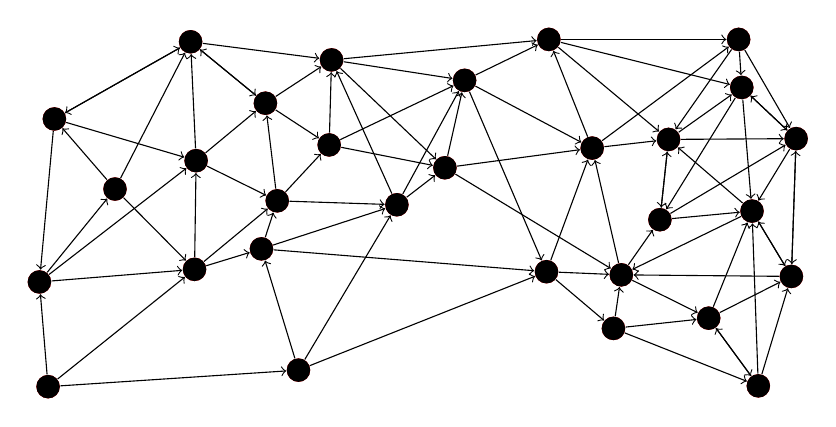
\begin{tikzpicture}
            \tikzstyle{before}=[circle,fill=black!20,inner sep=3pt]
            \tikzstyle{active}=[circle,fill=red,inner sep=3pt]
            \tikzstyle{after}=[circle,fill=black,inner sep=3pt]
            \node [before] (a)  at (0.45, 0.16) {}; \node<1> [active] at (0.45, 0.16) {}; \node<2-> [after] at (0.45, 0.16) {};
            \node [before] (b)  at (0.34, 1.49) {}; \node<2> [active] at (0.34, 1.49) {}; \node<3-> [after] at (0.34, 1.49) {};
            \node [before] (c)  at (2.31, 1.65) {}; \node<2> [active] at (2.31, 1.65) {}; \node<3-> [after] at (2.31, 1.65) {};
            \node [before] (d)  at (3.63, 0.37) {}; \node<2> [active] at (3.63, 0.37) {}; \node<3-> [after] at (3.63, 0.37) {};
            \node [before] (e)  at (1.30, 2.67) {}; \node<3> [active] at (1.30, 2.67) {}; \node<4-> [after] at (1.30, 2.67) {};
            \node [before] (f)  at (2.33, 3.03) {}; \node<3> [active] at (2.33, 3.03) {}; \node<4-> [after] at (2.33, 3.03) {};
            \node [before] (g)  at (0.53, 3.56) {}; \node<4> [active] at (0.53, 3.56) {}; \node<5-> [after] at (0.53, 3.56) {};
            \node [before] (h)  at (2.26, 4.54) {}; \node<4> [active] at (2.26, 4.54) {}; \node<5-> [after] at (2.26, 4.54) {};
            \node [before] (i)  at (3.36, 2.52) {}; \node<3> [active] at (3.36, 2.52) {}; \node<4-> [after] at (3.36, 2.52) {};
            \node [before] (j)  at (3.16, 1.91) {}; \node<3> [active] at (3.16, 1.91) {}; \node<4-> [after] at (3.16, 1.91) {};
            \node [before] (k)  at (4.88, 2.47) {}; \node<3> [active] at (4.88, 2.47) {}; \node<4-> [after] at (4.88, 2.47) {};
            \node [before] (l)  at (6.78, 1.62) {}; \node<3> [active] at (6.78, 1.62) {}; \node<4-> [after] at (6.78, 1.62) {};
            \node [before] (m)  at (3.21, 3.76) {}; \node<4> [active] at (3.21, 3.76) {}; \node<5-> [after] at (3.21, 3.76) {};
            \node [before] (n)  at (4.02, 3.23) {}; \node<4> [active] at (4.02, 3.23) {}; \node<5-> [after] at (4.02, 3.23) {};
            \node [before] (o)  at (4.05, 4.31) {}; \node<4> [active] at (4.05, 4.31) {}; \node<5-> [after] at (4.05, 4.31) {};
            \node [before] (p)  at (5.74, 4.05) {}; \node<4> [active] at (5.74, 4.05) {}; \node<5-> [after] at (5.74, 4.05) {};
            \node [before] (q)  at (5.49, 2.94) {}; \node<4> [active] at (5.49, 2.94) {}; \node<5-> [after] at (5.49, 2.94) {};
            \node [before] (r)  at (7.36, 3.19) {}; \node<4> [active] at (7.36, 3.19) {}; \node<5-> [after] at (7.36, 3.19) {};
            \node [before] (s)  at (7.73, 1.58) {}; \node<4> [active] at (7.73, 1.58) {}; \node<5-> [after] at (7.73, 1.58) {};
            \node [before] (t)  at (7.63, 0.90) {}; \node<4> [active] at (7.63, 0.90) {}; \node<5-> [after] at (7.63, 0.90) {};
            \node [before] (u)  at (6.81, 4.57) {}; \node<5> [active] at (6.81, 4.57) {}; \node<6-> [after] at (6.81, 4.57) {};
            \node [before] (v)  at (9.22, 4.57) {}; \node<5> [active] at (9.22, 4.57) {}; \node<6-> [after] at (9.22, 4.57) {};
            \node [before] (w)  at (8.33, 3.30) {}; \node<5> [active] at (8.33, 3.30) {}; \node<6-> [after] at (8.33, 3.30) {};
            \node [before] (x)  at (8.22, 2.28) {}; \node<5> [active] at (8.22, 2.28) {}; \node<6-> [after] at (8.22, 2.28) {};
            \node [before] (y)  at (8.84, 1.03) {}; \node<5> [active] at (8.84, 1.03) {}; \node<6-> [after] at (8.84, 1.03) {};
            \node [before] (z)  at (9.47, 0.17) {}; \node<5> [active] at (9.47, 0.17) {}; \node<6-> [after] at (9.47, 0.17) {};
            \node [before] (aa) at (9.26, 3.96) {}; \node<6> [active] at (9.26, 3.96) {}; \node<7-> [after] at (9.26, 3.96) {};
            \node [before] (bb) at (9.95, 3.31) {}; \node<6> [active] at (9.95, 3.31) {}; \node<7-> [after] at (9.95, 3.31) {};
            \node [before] (cc) at (9.39, 2.39) {}; \node<6> [active] at (9.39, 2.39) {}; \node<7-> [after] at (9.39, 2.39) {};
            \node [before] (dd) at (9.89, 1.56) {}; \node<6> [active] at (9.89, 1.56) {}; \node<7-> [after] at (9.89, 1.56) {};

            % Round 1
            \draw<1> [->] (a) -- (b);
            \draw<1> [->] (a) -- (c);
            \draw<1> [->] (a) -- (d);
            % Round 2
            \draw<2> [->] (b) -- (e);
            \draw<2> [->] (b) -- (c);
            \draw<2> [->] (b) -- (f);
            \draw<2> [->] (c) -- (f);
            \draw<2> [->] (c) -- (i);
            \draw<2> [->] (c) -- (j);
            \draw<2> [->] (d) -- (j);
            \draw<2> [->] (d) -- (k);
            \draw<2> [->] (d) -- (l);
            % Round 3
            \draw<3> [->] (e) -- (g);
            \draw<3> [->] (e) -- (h);
            \draw<3> [->] (e) -- (c);
            \draw<3> [->] (f) -- (h);
            \draw<3> [->] (f) -- (m);
            \draw<3> [->] (f) -- (i);
            \draw<3> [->] (i) -- (m);
            \draw<3> [->] (i) -- (n);
            \draw<3> [->] (i) -- (k);
            \draw<3> [->] (j) -- (i);
            \draw<3> [->] (j) -- (k);
            \draw<3> [->] (j) -- (l);
            \draw<3> [->] (k) -- (o);
            \draw<3> [->] (k) -- (p);
            \draw<3> [->] (k) -- (q);
            \draw<3> [->] (l) -- (r);
            \draw<3> [->] (l) -- (s);
            \draw<3> [->] (l) -- (t);
            % Round 4
            \draw<4> [->] (g) -- (b);
            \draw<4> [->] (g) -- (f);
            \draw<4> [->] (g) -- (h);
            \draw<4> [->] (h) -- (g);
            \draw<4> [->] (h) -- (m);
            \draw<4> [->] (h) -- (o);
            \draw<4> [->] (m) -- (h);
            \draw<4> [->] (m) -- (o);
            \draw<4> [->] (m) -- (n);
            \draw<4> [->] (n) -- (o);
            \draw<4> [->] (n) -- (p);
            \draw<4> [->] (n) -- (q);
            \draw<4> [->] (o) -- (u);
            \draw<4> [->] (o) -- (p);
            \draw<4> [->] (o) -- (q);
            \draw<4> [->] (p) -- (u);
            \draw<4> [->] (p) -- (r);
            \draw<4> [->] (p) -- (l);
            \draw<4> [->] (q) -- (p);
            \draw<4> [->] (q) -- (r);
            \draw<4> [->] (q) -- (s);
            \draw<4> [->] (r) -- (u);
            \draw<4> [->] (r) -- (v);
            \draw<4> [->] (r) -- (w);
            \draw<4> [->] (s) -- (r);
            \draw<4> [->] (s) -- (x);
            \draw<4> [->] (s) -- (y);
            \draw<4> [->] (t) -- (s);
            \draw<4> [->] (t) -- (y);
            \draw<4> [->] (t) -- (z);
            % Round 5
            \draw<5> [->] (u) -- (v);
            \draw<5> [->] (u) -- (aa);
            \draw<5> [->] (u) -- (w);
            \draw<5> [->] (v) -- (w);
            \draw<5> [->] (v) -- (aa);
            \draw<5> [->] (v) -- (bb);
            \draw<5> [->] (w) -- (aa);
            \draw<5> [->] (w) -- (bb);
            \draw<5> [->] (w) -- (x);
            \draw<5> [->] (x) -- (w);
            \draw<5> [->] (x) -- (bb);
            \draw<5> [->] (x) -- (cc);
            \draw<5> [->] (y) -- (cc);
            \draw<5> [->] (y) -- (dd);
            \draw<5> [->] (y) -- (z);
            \draw<5> [->] (z) -- (y);
            \draw<5> [->] (z) -- (cc);
            \draw<5> [->] (z) -- (dd);
            % Round 6
            \draw<6> [->] (aa) -- (bb);
            \draw<6> [->] (aa) -- (cc);
            \draw<6> [->] (aa) -- (x);
            \draw<6> [->] (bb) -- (aa);
            \draw<6> [->] (bb) -- (dd);
            \draw<6> [->] (bb) -- (cc);
            \draw<6> [->] (cc) -- (w);
            \draw<6> [->] (cc) -- (s);
            \draw<6> [->] (cc) -- (dd);
            \draw<6> [->] (dd) -- (bb);
            \draw<6> [->] (dd) -- (cc);
            \draw<6> [->] (dd) -- (s);
        \end{tikzpicture}
    \end{center}%
    \uncover<7>{Eventually reaches all nodes (with high probability).}
\end{frame}
\inlineslide{s:gossip}{}\label{l:gossip}

% what state must a recipient maintain in order to eliminate duplicates?
% the entire message? a unique message ID? a sequence number? (what assumptions does this require making about the sender?)

%\supervision{
%    Write pseudocode for a gossip-based implementation of reliable broadcast.
%}{
%    TODO do we want this?
%}

Now that we have reliable broadcast (using eager reliable broadcast or a gossip protocol), we can build FIFO, causal, or total order broadcast on top of it.
Let's start with FIFO broadcast.

\begin{frame}
    \label{s:fifo-algorithm}
    \frametitle{FIFO broadcast algorithm}
    \footnotesize
    \begin{algorithmic}
        \On{initialisation}
            \State $\mathit{sendSeq} := 0;\; \mathit{delivered} := \langle 0, 0, \dots, 0 \rangle;\; \mathit{buffer} := \{\}$
        \EndOn
        \State
        \On{request to broadcast $m$ at node $N_i$}
            \State send $(i, \mathit{sendSeq}, m)$ via reliable broadcast
            \State $\mathit{sendSeq} := \mathit{sendSeq} + 1$
        \EndOn
        \State
        \On{receiving $\mathit{msg}$ from reliable broadcast at node $N_i$}
            \State $\mathit{buffer} := \mathit{buffer} \cup \{\mathit{msg}\}$
            \While{$\exists \mathit{sender}, m.\; (\mathit{sender}, \mathit{delivered}[\mathit{sender}], m) \in \mathit{buffer}$}
                \State deliver $m$ to the application
                \State $\mathit{delivered}[\mathit{sender}] := \mathit{delivered}[\mathit{sender}] + 1$
            \EndWhile
        \EndOn
    \end{algorithmic}
\end{frame}
\inlineslide{s:fifo-algorithm}{}\label{l:fifo-algorithm}

Each FIFO broadcast message sent by node $N_i$ is tagged with the sending node number $i$ and a sequence number that is 0 for the first message sent by $N_i$, 1 for the second message, and so on.
The local state at each node consists of the sequence number \emph{sendSeq} (counting the number of messages broadcast by this node), \emph{delivered} (a vector with one entry per node, counting the number of messages from each sender that this node has delivered), and \emph{buffer} (a buffer for holding back messages until they are ready to be delivered).
The algorithm checks for messages from any sender that match the expected next sequence number, and then increments that number, ensuring that messages from each particular sender are delivered in order of increasing sequence number.

The causal broadcast algorithm is somewhat similar to FIFO broadcast; instead of attaching a sequence number to every message that is broadcast, we attach a vector of integers.
This algorithm is sometimes called a \emph{vector clock} algorithm, even though it is quite different from the algorithm on \autoref{l:vector-definition}.
In the vector clock algorithm from \autoref{l:vector-definition} the vector elements count the number of \emph{events} that have occurred at each node, while in the causal broadcast algorithm, the vector elements count the number of \emph{messages} from each sender that have been delivered.

\begin{frame}
    \label{s:causal-algorithm}
    \frametitle{Causal broadcast algorithm}
    \footnotesize
    \begin{algorithmic}
        \On{initialisation}
            \State $\mathit{sendSeq} := 0;\; \mathit{delivered} := \langle 0, 0, \dots, 0 \rangle;\; \mathit{buffer} := \{\}$
        \EndOn
        \State
        \On{request to broadcast $m$ at node $N_i$}
            \State $\mathit{deps} := \mathit{delivered}; \mathit{deps}[i] := sendSeq$
            \State send $(i, \mathit{deps}, m)$ via reliable broadcast
            \State $\mathit{sendSeq} := \mathit{sendSeq} + 1$
        \EndOn
        \State
        \On{receiving $\mathit{msg}$ from reliable broadcast at node $N_i$}
            \State $\mathit{buffer} := \mathit{buffer} \cup \{\mathit{msg}\}$
            \While{$\exists (\mathit{sender}, \mathit{deps}, m) \in \mathit{buffer}.\; \mathit{deps} \le \mathit{delivered}$}
                \State deliver $m$ to the application
                \State $\mathit{buffer} := \mathit{buffer} \setminus \{(\mathit{sender}, \mathit{deps}, m)\}$
                \State $\mathit{delivered}[\mathit{sender}] := \mathit{delivered}[\mathit{sender}] + 1$
            \EndWhile
        \EndOn
    \end{algorithmic}
\end{frame}
\inlineslide{s:causal-algorithm}{}\label{l:causal-algorithm}

\againframe<1>{vector-ordering}

The local state at each node consists of \emph{sendSeq}, \emph{delivered}, and \emph{buffer}, which have the same meaning as in the FIFO broadcast algorithm.
When a node wants to broadcast a message, we attach the sending node number $i$ and $\mathit{deps}$, a vector indicating the \emph{causal dependencies} of that message.
We construct $\mathit{deps}$ by taking a copy of $\mathit{delivered}$, the vector that counts how many messages from each sender have been delivered at this node.
This indicates that all messages that have been delivered locally prior to this broadcast must appear before the broadcast message in the causal order.
We then update the sending node's own element of this vector to equal $\mathit{sendSeq}$, which ensures that each message broadcast by this node has a causal dependency on the previous message broadcast by the same node.

When receiving a message, the algorithm first adds it to the buffer like in FIFO broadcast, and then searches the buffer for any messages that are ready to be delivered.
The comparison $\mathit{deps} \le \mathit{delivered}$ uses the $\le$ operator on vectors defined on \autoref{l:vector-ordering}.
This comparison is true if this node has already delivered all of the messages that must precede this message in the causal order.
Any messages that are causally ready are then delivered to the application and removed from the buffer, and the appropriate element of the $\mathit{delivered}$ vector is incremented.

\begin{frame}
    \label{s:total-bcast-alg}
    \frametitle{Total order broadcast algorithms}
    \textbf{Single leader} approach:
    \begin{itemize}
        \item One node is designated as leader (sequencer)
        \item To broadcast message, send it to the leader;\\ leader broadcasts it via FIFO broadcast.\pause
        \item Problem: leader crashes $\Longrightarrow$ no more messages delivered
        \item Changing the leader safely is difficult\\[1em]
    \end{itemize}\pause
    \textbf{Lamport clocks} approach:
    \begin{itemize}
        \item Attach Lamport timestamp to every message
        \item Deliver messages in total order of timestamps\pause
        \item Problem: how do you know if you have seen all messages with timestamp $< T$?
            Need to use FIFO links and wait for message with timestamp $\ge T$ from \emph{every} node
    \end{itemize}
\end{frame}
\inlineslide{s:total-bcast-alg}{}\label{l:total-bcast-alg}

Finally, total order broadcast (and FIFO-total order broadcast) are trickier.
Two simple approaches are outlined on \autoref{l:total-bcast-alg}, one based on a designated leader node, and a leaderless algorithm using Lamport timestamps.
However, neither of these approaches is fault tolerant: in both cases, the crash of a single node can stop all other nodes from being able to deliver messages.
In the single-leader approach, the leader is a single point of failure.
We will return to the problem of fault-tolerant total order broadcast in \autoref{sec:consensus}.

\supervision{
    Give pseudocode for an algorithm that implements FIFO-total order broadcast using Lamport clocks.
    You may assume that each node has a unique ID, and that the set of all node IDs is known.
    Further assume that the underlying network provides reliable FIFO broadcast.
    [\href{https://www.cl.cam.ac.uk/teaching/exams/pastpapers/y2020p5q8.pdf}{2020 Paper 5 Question 8}]
}{
    Each node maintains its state in the following variables:
    \begin{itemize}
        \item \texttt{procs}: set of all node IDs in the group
        \item \texttt{proc}: ID of the current node
        \item \texttt{counter}: an integer, initially zero
        \item \texttt{minLamport}: a map where the keys are node IDs and values are integers (initial value 0 for each node)
        \item \texttt{holdback}: a priority queue where keys are (integer, node ID) pairs and values are messages; the \texttt{getMin()} method returns the entry with the smallest key according to lexicographic order on (integer, node ID) pairs
    \end{itemize}
    \inputminted{js}{code/lamport-broadcast.js}
}

\section{Replication}\label{sec:replication}

\begin{frame}
    \begin{center}
        {\Large{\color{darkblue}{Replication}}} \\[2em]
        \mydetails
    \end{center}
\end{frame}

We will now turn to the problem of \emph{replication}, which means to maintain a copy of the same data on multiple nodes, each of which is called a \emph{replica}.
Replication is a standard feature of many distributed databases, filesystems, and other storage systems.
It is one of the main mechanisms we have for achieving \emph{fault tolerance}: if one replica becomes faulty, we can continue accessing the copies of the data on other replicas.

\begin{frame}
    \label{s:replication-intro}
    \frametitle{Replication}
    \begin{itemize}
        \item Keeping a copy of the same data on multiple nodes
        \item Databases, filesystems, caches, \dots
        \item A node that has a copy of the data is called a \textbf{replica}\pause
        \item If some replicas are faulty, others are still accessible
        \item Spread load across many replicas\pause
        \item Easy if the data doesn't change: just copy it
        \item We will focus on data changes\\[1em]\pause
    \end{itemize}
    Compare to \textbf{RAID} (Redundant Array of Independent Disks):\\replication within a single computer
    \begin{itemize}
        \item RAID has single controller; in distributed system, each node acts independently
        \item Replicas can be distributed around the world, near users
    \end{itemize}
\end{frame}
\inlineslide{s:replication-intro}{}\label{l:replication-intro}

\subsection{Manipulating remote state}\label{sec:remote-state}

If the data doesn't change, replication is easy, since it just requires making a one-time copy of the data.
Therefore, the main problem in replication is managing changes to the data.
Before we get into the details of replication, let's look at how data changes happen in a distributed system.

\begin{frame}
    \label{s:retry-increment}
    \frametitle{Retrying state updates}
    \framebox{
        \begin{minipage}{10cm}
            \textbf{User A}: The moon is not actually made of cheese!\\[0.5em]
            \fbox{\thumbsup~Like}\hspace{1em} 12,300 people like this.
        \end{minipage}
    }
    \begin{center}
        \begin{tikzpicture}
            \node at (10,-0.1) {}; % placeholder
            \node [rectangle,fill=red!10,draw] (gen1) at (0,4) {client};
            \node [rectangle,fill=red!10,draw] (gen2) at (8,4) {\storageSymbol};
            \draw (gen1) -- (0,0);
            \draw (gen2) -- (8,0);
            \draw<2-> [bigarrow] (0,3.3) -- node [above,sloped] {increment post.likes} node [at end,right] {12,301} (8,2.9);
            \draw<2-> [messageloss] (8,2.6) -- node [above,sloped] {ack} (2,2.3);
            \draw<3-> [bigarrow] (0,1.3) -- node [above,sloped] {increment post.likes} node [at end,right] {12,302} (8,0.9);
            \draw<3-> [messageloss] (8,0.6) -- node [above,sloped] {ack} (2,0.3);
        \end{tikzpicture}
    \end{center}%
    \uncover<4->{Deduplicating requests requires that the database tracks which requests it has already seen (in stable storage)}
\end{frame}
\inlineslide{s:retry-increment}{}\label{l:retry-increment}

Let's consider as example the act of ``liking'' a status update on a social network.
When you click the ``like'' button, the fact that you have liked it, and the number of people who have liked it, need to be stored somewhere so that they can be displayed to you and to other users.
This usually happens in a database on the social network's servers.
We can consider the data stored in a database to be its \emph{state}.

A request to update the database may be lost in the network, or an acknowledgement that an update has been performed might be lost.
As usual, we can improve reliability by retrying the request.
However, if we are not careful, the retry could lead to the request being processed multiple times, leading to an incorrect state in the database.

\begin{frame}[plain]
    \label{s:negative-followers}
    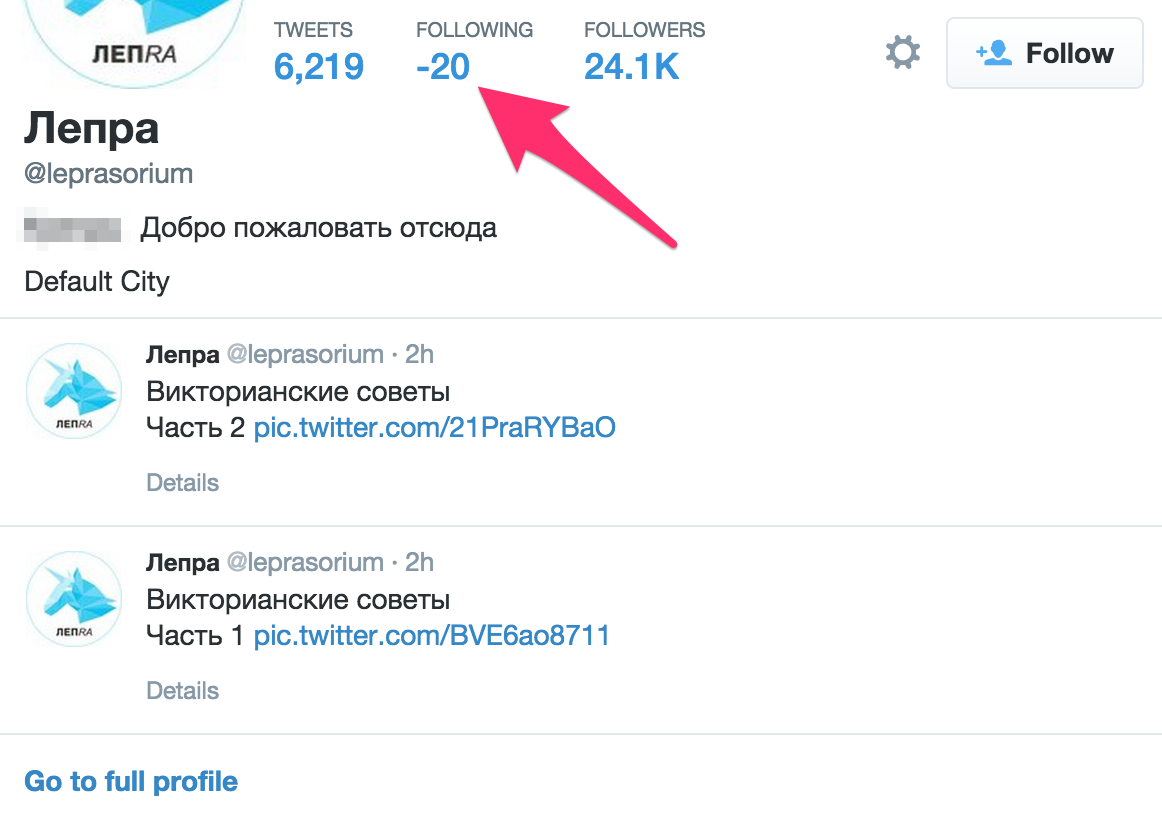
\includegraphics[width=12cm]{images/negative-followers.png}
\end{frame}
\inlineslide{s:negative-followers}{}\label{l:negative-followers}

Lest you think this is a purely hypothetical problem, consider \autoref{l:negative-followers}, a genuine (I promise!) screenshot of Twitter that I made in 2014, which shows the profile of a user who is apparently following a negative number of people.
I don't have insight into Twitter's internals to know exactly what happened here, but my guess is that this person used to follow several people, then unfollowed them, and due to a network problem during the unfollowing process, the decrement of the follow counter was retried, resulting in more decrements than the user was originally following.

If following a negative number of people seems like a trivial problem, then instead of decrementing a follow counter, consider the act of deducting {\textsterling}1,000 from your bank account balance.
The database operation is essentially the same, but performing this operation too many times has the potential to make you rather unhappy.

To prevent an update from taking effect multiple times, we need to deduplicate requests.
More formally speaking, we need to make requests \emph{idempotent}.

\begin{frame}
    \label{s:idempotence}
    \frametitle{Idempotence}
    A function $f$ is idempotent if $f(x) = f(f(x))$.
    \begin{itemize}
        \item \textbf{Not idempotent:} $f(\mathit{likeCount}) = \mathit{likeCount} + 1$
        \item \textbf{Idempotent:} $f(\mathit{likeSet}) = \mathit{likeSet} \cup \{\mathit{userID}\}$
    \end{itemize}
    Idempotent requests can be retried safely.\\[1em]\pause
    Choice of retry behaviour:
    \begin{itemize}
        \item \textbf{At-most-once} semantics:\\
            send request, don't retry, update may not happen
        \item \textbf{At-least-once} semantics:\\
            retry request until acknowledged, may repeat update
        \item \textbf{Exactly-once} semantics:\\
            retry + idempotence or deduplication
    \end{itemize}
\end{frame}
\inlineslide{s:idempotence}{}\label{l:idempotence}

Incrementing a counter is not idempotent, but adding an element to a set is.
Therefore, if a counter is required (as in the number of likes), it might be better to actually maintain the set of elements in the database, and to derive the counter value from the set by computing its cardinality.
In a crash-recovery system model, we can deduplicate requests storing them (or some metadata about requests, such as a vector clock) in stable storage, so that duplicates can be accurately detected even after a crash.

An idempotent update can safely be retried, because performing it several times has the same effect as performing it once.
Idempotence allows an update to have \emph{exactly-once} semantics: that is, the update may actually be applied multiple times, but the effect is the same as if it had been applied exactly once.
Idempotence is a very useful property in practical systems, and it is often found in the context of RPC (\autoref{sec:rpc}), where retries are often unavoidable.


However, idempotence has a limitation that becomes apparent when there are multiple updates in progress.
On \autoref{l:retry-union}, client 1 adds a user ID to the set of likes for a post, but the acknowledgement is lost.
Client 2 reads the set of likes from the database (including the user ID added by client 1), and then makes a request to remove the user ID again.
Meanwhile, client 1 retries its request, unaware of the update made by client 2.
The retry therefore has the effect of adding the user ID to the set again.
This is unexpected since client 2 observed client 1's change, so the removal happened causally after the addition of the set element, and therefore we might expect that in the final state, the user ID should \emph{not} be present in the set.
In this case, the fact that adding an element to a set is idempotent is not sufficient to make the retry safe.

\begin{frame}
    \label{s:retry-union}
    \frametitle{Adding and then removing again}
    \begin{center}
        \begin{tikzpicture}
            \node [rectangle,fill=red!10,draw] (node1) at (0,4) {client 1};
            \node [rectangle,fill=red!10,draw] (node2) at (4,4) {\storageSymbol};
            \node [rectangle,fill=red!10,draw] (node3) at (8,4) {client 2};
            \draw (node1) -- (0,-0.4);
            \draw (node2) -- (4,-0.4);
            \draw (node3) -- (8,-0.4);
            \draw<2-> [bigarrow] (0,3.3) -- node [above,sloped] {$f$: add like} (4,2.9);
            \draw<2-> [messageloss] (4,2.6) -- node [above,sloped] {ack} (1,2.3);
            \draw<3-> [bigarrow] (4,2.3) -- node [above,sloped] {set of likes} (8,1.9);
            \draw<4-> [bigarrow] (8,1.6) -- node [above,sloped] {$g$: unlike} (4,1.2);
            \draw<4-> [bigarrow] (4,0.9) -- node [above,sloped] {ack} (8,0.6);
            \draw<5-> [bigarrow] (0,1.0) -- node [above,sloped] {$f$: add like} (4,0.6);
            \draw<5-> [bigarrow] (4,0.3) -- node [above,sloped] {ack} (0,-0.1);
        \end{tikzpicture}
    \end{center}%
    \uncover<2->{$f(\mathit{likes}) = \mathit{likes} \cup \{\mathit{userID}\}$}\\%
    \uncover<4->{$g(\mathit{likes}) = \mathit{likes} \setminus \{\mathit{userID}\}$}\\%
    \uncover<6->{\textbf{Idempotent?} $f(f(x)) = f(x)$ but $f(g(f(x)) \neq g(f(x))$}
\end{frame}
\inlineslide{s:retry-union}{}\label{l:retry-union}

A similar problem occurs on \autoref{l:add-remove}, in which we have two replicas.
In the first scenario a client first adds $x$ to both replicas of the database, then tries to remove $x$ again from both.
However, the remove request to replica $B$ is lost, and the client crashes before it is able to retry.
In the second scenario a client tries to add $x$ to both replicas, but the request to replica $A$ is lost, and again the client crashes.

% TODO: change "add(x)" notation to "(add, x)" here and similarly on many following slides in this lecture and lecture 7
\begin{frame}
    \label{s:add-remove}
    \frametitle{Another problem with adding and removing}
    \begin{center}
        \begin{tikzpicture}
            \node [rectangle,fill=red!10,draw] (node1) at (0,4.5) {client};
            \node [rectangle,fill=red!10,draw] (node2) at (4,4.5) {\storageSymbol}; \node [yshift=-0.2cm] at (node2) {$A$};
            \node [rectangle,fill=red!10,draw] (node3) at (8,4.5) {\storageSymbol}; \node [yshift=-0.2cm] at (node3) {$B$};
            \draw [crash] (node1) -- (0,1.6);
            \draw (node2) -- (4,1.5);
            \draw (node3) -- (8,1.5);
            \draw<2-> [bigarrow] (0,4.0) -- node [above,near start,sloped,yshift=-0.1cm] {$\mathsf{add}(x)$} (8,3.2);
            \draw<2-> [bigarrow] (0,3.9)
                .. controls (1,3.8) and (1,3.3) .. (2,3.2)
                -- node [above,sloped,yshift=-0.1cm] {$\mathsf{add}(x)$} (4,3.0);
            \draw<3-> [messageloss] (0,2.8) -- node [above,near start,sloped,yshift=-0.1cm] {$\mathsf{remove}(x)$} (6,2.2);
            \draw<3-> [bigarrow] (0,2.7)
                .. controls (1,2.6) and (1,2.1) .. (2,2.0)
                -- node [above,sloped,yshift=-0.1cm,pos=0.4] {$\mathsf{remove}(x)$} (4,1.8);
        \end{tikzpicture}\\[1em]%
        \uncover<4->{Final state ($x \notin A,\; x \in B$) is the same as in this case:}\\[1em]%
        \begin{tikzpicture}
            \node at (0,0) {}; \node at (0,5) {}; % placeholder
            \node<5-> [rectangle,fill=red!10,draw] (node1) at (0,4.5) {client};
            \node<5-> [rectangle,fill=red!10,draw] (node2) at (4,4.5) {\storageSymbol}; \node<5-> [yshift=-0.2cm] at (node2) {$A$};
            \node<5-> [rectangle,fill=red!10,draw] (node3) at (8,4.5) {\storageSymbol}; \node<5-> [yshift=-0.2cm] at (node3) {$B$};
            \draw<5-> [crash] (node1) -- (0,2.9);
            \draw<5-> (node2) -- (4,2.8);
            \draw<5-> (node3) -- (8,2.8);
            \draw<5-> [bigarrow] (0,4.0) -- node [above,near start,sloped,yshift=-0.1cm] {$\mathsf{add}(x)$} (8,3.2);
            \draw<5-> [messageloss] (0,3.9)
                .. controls (1,3.8) and (1,3.3) .. (2,3.2)
                -- node [at start,above,sloped,yshift=-0.1cm] {$\mathsf{add}(x)$} (3.5,3.05);
        \end{tikzpicture}
    \end{center}%
\end{frame}
\inlineslide{s:add-remove}{}\label{l:add-remove}

In both scenarios the outcome is the same: $x$ is present on replica $B$, and absent from replica $A$.
Yet the intended effect is different: in the first scenario, the client wanted $x$ to be removed from both replicas, whereas in the second scenario, the client wanted $x$ to be present on both replicas.
When the two replicas reconcile their inconsistent states, we want them to both end up in the state that the client intended.
However, this is not possible if the replicas cannot distinguish between these two scenarios.

To solve this problem, we can do two things.
First, we attach a logical timestamp to every update operation, and store that timestamp in the database as part of the data written by the update.
Second, when asked to remove a record from the database, we don't actually remove it, but rather write a special type of update (called a \emph{tombstone}) marking it as deleted.
On \autoref{l:tombstones}, records containing $\mathsf{false}$ are tombstones.

\begin{frame}
    \label{s:tombstones}
    \frametitle{Timestamps and tombstones}
    \begin{center}
        \begin{tikzpicture}
            \node [rectangle,fill=red!10,draw] (node1) at (0,5) {client};
            \node [rectangle,fill=red!10,draw] (node2) at (4,5) {\storageSymbol}; \node [yshift=-0.2cm] at (node2) {$A$};
            \node [rectangle,fill=red!10,draw] (node3) at (8,5) {\storageSymbol}; \node [yshift=-0.2cm] at (node3) {$B$};
            \draw [crash] (node1) -- (0,0.6);
            \draw (node2) -- (4,0.5);
            \draw (node3) -- (8,0.5);
            \draw [bigarrow] (0,4.0)
                -- node [left,at start] {$t_1$}
                   node [above,near start,sloped] {$(t_1, \mathsf{add}(x))$}
                   node [right,at end] {$\{x \mapsto (t_1, \mathsf{true})\}$} (8,3.2);
            \draw [bigarrow] (0,3.9)
                .. controls (1,3.8) and (1,3.1) .. (2,3.0)
                -- node [above,sloped,near start] {$(t_1, \mathsf{add}(x))$}
                   node [right,at end] {$\{x \mapsto (t_1, \mathsf{true})\}$} (4,2.8);
            \draw<2-> [messageloss] (0,2.0)
                -- node [left,at start] {$t_2$}
                   node [above,near start,sloped] {$(t_2, \mathsf{remove}(x))$} (6,1.4);
            \draw<2-> [bigarrow] (0,1.9)
                .. controls (1,1.8) and (1,1.1) .. (2,1.0)
                -- node [above,sloped,near start] {$(t_2, \mathsf{remove}(x))$}
                   node [right,at end] {$\{x \mapsto (t_2, \mathsf{false})\}$} (4,0.8);
        \end{tikzpicture}
    \end{center}%
    \uncover<3->{``$\mathsf{remove}(x)$'' doesn't actually remove $x$:
    it labels $x$ with ``$\mathsf{false}$'' to indicate it is invisible (a \textbf{tombstone})}\\[0.5em]%
    \uncover<4->{Every record has \textbf{logical timestamp} of last write}\\[1em]
\end{frame}
\inlineslide{s:tombstones}{}\label{l:tombstones}

In many replicated systems, replicas run a protocol to detect and reconcile any differences (this is called \emph{anti-entropy}), so that the replicas eventually hold consistent copies of the same data.
Thanks to tombstones, the anti-entropy process can tell the difference between a record that has been deleted and a record that has not yet been created.
And thanks to timestamps, we can tell which version of a record is older and which is newer.
The anti-entropy process then keeps the newer and discards the older record.

This approach also helps address the problem on \autoref{l:retry-union}: a retried request has the same timestamp as the original request, so a retry will not overwrite a value written by a causally later request with a greater timestamp.

\begin{frame}
    \label{s:reconcile}
    \frametitle{Reconciling replicas}
    \begin{center}
        Replicas periodically communicate among themselves\\to check for any inconsistencies.\\[1em]
        \begin{tikzpicture}
            \node [rectangle,fill=red!10,draw] (node2) at (0,5) {\storageSymbol}; \node [yshift=-0.2cm] at (node2) {$A$};
            \node [rectangle,fill=red!10,draw] (node3) at (8,5) {\storageSymbol}; \node [yshift=-0.2cm] at (node3) {$B$};
            \node (left1) at (0,3.5) {$\{x \mapsto (t_2, \mathsf{false})\}$};
            \node (right1) at (8,3.5) {$\{x \mapsto (t_1, \mathsf{true})\}$};
            \node<3-> (left2) at (0,2.0) {$\{x \mapsto (t_2, \mathsf{false})\}$};
            \node<3-> (right2) at (8,2.0) {$\{x \mapsto (t_2, \mathsf{false})\}$};
            \draw<2-> [doublebigarrow] (left1) -- node [above] {reconcile state} node [below] {(anti-entropy)} (right1);
            \draw<3-> [bigarrow] (left1) -- (left2);
            \draw<3-> [bigarrow] (right1) -- (right2);
            \node<3-> at (4,2.0) {$t_1 < t_2$};
            \node at (0,1.8) {}; % placeholder
        \end{tikzpicture}\\[1em]
        \uncover<4->{Propagate the record with the latest timestamp,\\discard the records with earlier timestamps\\(for a given key).}
    \end{center}%
\end{frame}
\inlineslide{s:reconcile}{}\label{l:reconcile}

The technique of attaching a timestamp to every update is also useful for handling concurrent updates to a \emph{register} (a replicated variable whose value can be updated).
For example, in a key-value store, each key has an associated register.
On \autoref{l:concurrent-writes}, client~1 wants to set the register for key $x$ to the value $v_1$ (with timestamp $t_1$), while concurrently client~2 wants to set the register for the same key $x$ to the value $v_2$ (with timestamp $t_2$).
Replica $A$ receives $v_2$ first and $v_1$ second, while replica $B$ receives the updates in the opposite order.
To ensure that both replicas end up in the same state, we rely not on the order in which they receive requests, but the order of their timestamps.

\begin{frame}
    \label{s:concurrent-writes}
    \frametitle{Concurrent writes by different clients}
    \begin{center}
        \begin{tikzpicture}
            \node [rectangle,fill=red!10,draw] (node1) at (0,3) {client 1};
            \node [rectangle,fill=red!10,draw] (node2) at (3,3) {\storageSymbol}; \node [yshift=-0.2cm] at (node2) {$A$};
            \node [rectangle,fill=red!10,draw] (node3) at (6,3) {\storageSymbol}; \node [yshift=-0.2cm] at (node3) {$B$};
            \node [rectangle,fill=red!10,draw] (node4) at (9,3) {client 2};
            \draw (node1) -- (0,0);
            \draw (node2) -- (3,0);
            \draw (node3) -- (6,0);
            \draw (node4) -- (9,0);
            \draw<2-> [bigarrow] (0,2.0)
                -- node [left,at start] {$t_1$}
                   node [above,near start,sloped] {$(t_1, \mathsf{set}(x, v_1))$} (6,0.8);
            \draw<2-> [bigarrow] (0,1.9)
                .. controls (1,1.7) and (1,0.7) .. (2,0.5) -- (3,0.3);
            \draw<3-> [bigarrow] (9,2.0)
                -- node [right,at start] {$t_2$}
                   node [above,near start,sloped] {$(t_2, \mathsf{set}(x, v_2))$} (3,0.8);
            \draw<3-> [bigarrow] (9,1.9)
                .. controls (8,1.7) and (8,0.7) .. (7,0.5) -- (6,0.3);
        \end{tikzpicture}
    \end{center}%
    \begin{uncoverenv}<4->
        Two common approaches:
        \begin{itemize}
            \item \textbf{Last writer wins} (LWW) register:\\
                Use timestamps with total order (e.g. Lamport clock)\\
                Keep $v_2$ and discard $v_1$ if $t_2 > t_1$. Note: \textbf{data loss}!
            \item<5-> \textbf{Multi-value register}:\\
                Use timestamps with partial order (e.g. vector clock)\\
                $v_2$ replaces $v_1$ if $t_2 > t_1$; preserve both $\{v_1,v_2\}$ if $t_1 \parallel t_2$\\[1em]
        \end{itemize}
    \end{uncoverenv}
\end{frame}
\inlineslide{s:concurrent-writes}{}\label{l:concurrent-writes}

The details of this approach depend on the type of timestamps used.
If we use Lamport clocks (with the total order defined on \autoref{l:lamport-example}), two concurrent updates will be ordered arbitrarily, depending on how the timestamps happen to get assigned.
In this case, we get what is known as \emph{last writer wins} (LWW) semantics: the update with the greatest timestamp takes effect, and any concurrent updates with lower timestamps to the same key are discarded.
This approach is simple to work with, but it implies data loss when multiple updates are performed concurrently.
Whether or not this is a problem depends on the application: in some systems, discarding concurrent updates is fine.

When discarding concurrent updates is not acceptable, we need to use a type of timestamp that allows us to detect when updates happen concurrently, such as vector clocks.
With such partially ordered timestamps, we can tell when a new value should overwrite an old value (when the old update happened before the new update), and when several updates are concurrent, we can keep all of the concurrently written values.
These concurrently written values are called \emph{conflicts}, or sometimes \emph{siblings}.
The application can later merge conflicts back into a single value, as discussed in \autoref{sec:eventual-consistency}.

A downside of vector clocks is that they can become expensive: every client needs an entry in the vector, and in systems with large number of clients (or where clients assume a new identity every time they are restarted), these vectors can become large, potentially taking up more space than the data itself.
Further types of logical clocks, such as \emph{dotted version vectors} \citep{Preguica:2010}, have been developed to optimise this type of system.

\supervision{\label{q:cassandra}
    Apache Cassandra, a widely-used distributed database, uses a replication approach similar to the one described here.
    However, it uses physical timestamps instead of logical timestamps, as discussed here: \url{https://www.datastax.com/blog/why-cassandra-doesnt-need-vector-clocks}.
    % Archived blog post: https://perma.cc/MMQ9-R6ZC
    Write a critique of this blog post.
    What do you think of its arguments and why?
    What facts are missing from it?
    What recommendation would you make to someone considering using Cassandra?
}{
    The article conflates several different things.
    It explains the advantage of performing fine-grained updates (e.g. updating only one field of a user record rather than replacing the whole record), which may reduce the frequency of conflicts between writes and may improve performance.
    However, the granularity of updates has got nothing to do with the choice between physical or logical clocks.

    Major problems with physical clocks are left unmentioned in the article, in particular that they may be inconsistent with causality.
    For example, if a client reads the value for a key in the database, and writes back an updated value, it is possible that the write has no effect.
    This could happen if the client that previously wrote this key has a fast-running clock, and/or the client making the subsequent update has a slow-running clock, and so the second write's physical timestamp ends up being less than the previous write's timestamp.
    The article's claim that ``clock synchronisation is nice to have in a Cassandra cluster but not critical'' is completely wrong: clock sync is in fact crucial.

    If a client makes several successive writes to the same key, and the clock jumps backwards due to NTP stepping or a leap second, then it could happen that a later write fails to overwrite an earlier value because the later write has an earlier timestamp.
    In all of these cases, there is no error (the client believes that the database has stored the data) even though the data has in fact been discarded, not stored.
    This problem is discussed further in this article: \url{https://aphyr.com/posts/299-the-trouble-with-timestamps}

    The article explains that vector clocks allow the database to detect concurrently written values, giving the application the option of merging those values without data loss.
    However, as the article points out, this can be difficult for applications to do correctly.
    The alternative used by Cassandra, namely last-write-wins, simply discards all but one value when several values are written concurrently.
    This is certainly simpler, but the potential for data loss is not really acknowledged in this article.
    Moreover, the LWW conflict resolution strategy can be used even in a system that uses vector clocks, by using a merge function that discards all but one value.
    Using vector clocks opens the \emph{option} of merging concurrently written values, but it does not \emph{force} the application to be any more complicated than one based on LWW.
    Moreover, if detection of concurrent writes is not desired, Lamport clocks could be used instead of vector clocks: these would be fine for LWW semantics, and would avoid the problems of physical clocks.

    The article claims that Cassandra's approach is faster because an object does not need to be read in order to be updated.
    However, the choice of logical or physical clocks does not affect this aspect: even with logical clocks, a write that simply overwrites any existing value without reading its value (a so-called \emph{blind write}) can be performed without reading a record first.

    The only real reason I can see in favour of physical clocks is that they allow the API for clients to be simpler.
    If logical clocks are used, a write that depends on a prior read needs to propagate the logical timestamp from the read operation to the write operation, which means that they have to somehow be coupled in the client code.
    Using physical timestamps does not have this requirement.
    However, the article doesn't actually make this argument.

    In summary, the article does not make a convincing argument in favour of using physical time, and fails to acknowledge its risks.
    My recommendation for using Cassandra is that it's okay to use in situations where a record is only written once and then never updated (for example, for storing log files, where each line of the log is one record), because in that case the timestamp is irrelevant.
    However, any applications that update existing records in Cassandra are at risk of data loss if they encounter any problems with their clock synchronisation.
}

\subsection{Quorums}\label{sec:quorums}

As discussed at the start of this lecture, replication is useful since it allows us to improve the reliability of a system: when one replica is unavailable, the remaining replicas can continue processing requests.
Unavailability could be due to a faulty node (e.g.\ a crash or a hardware failure), due to a network partition (inability to reach a node over the network), or planned maintenance (e.g.\ rebooting a node to install software updates).

However, the details of how exactly the replication is performed have a big impact on the reliability of the system.
Without fault tolerance, having multiple replicas would make reliability \emph{worse}: the more replicas you have, the greater the probability that \emph{any one} of the replicas is faulty at any one time (assuming faults are not perfectly correlated).
However, if the system continues working despite some faulty replicas, then reliability improves: the probability that \emph{all} replicas are faulty at the same time is much lower than the probability of one replica being faulty.

\begin{frame}
    \label{s:fault-probability}
    \frametitle{Probability of faults}
    A replica may be \textbf{unavailable} due to network partition or node fault (e.g. crash, hardware problem).\\[1em]\pause
    Assume each replica has probability $p$ of being faulty or unavailable at any one time, and that faults are independent.\\
    {\footnotesize (Not actually true! But okay approximation for now.)}\\[1em]\pause
    Probability of \textbf{all} $n$ replicas being faulty: $p^n$\\
    Probability of $\ge 1$ out of $n$ replicas being faulty: $1-(1-p)^n$\\[1em]\pause
    Example with $p=0.01$:\\[0.5em]
    \rowcolors[]{2}{}{blue!10}
    \begin{tabular}{c|c|c|c}
        \hline
        replicas $n$ & $P(\ge 1 \text{ faulty})$ & $P(\ge \frac{n+1}{2}\text{ faulty})$ & $P(\text{all } n \text{ faulty})$ \\\hline
        1 & 0.01 & 0.01 & 0.01 \\
        3 & 0.03 & $3 \cdot 10^{-4}$ & $10^{-6}$ \\
        5 & 0.049 & $1 \cdot 10^{-5}$ & $10^{-10}$ \\
        100 & 0.63 & $6 \cdot 10^{-74}$ & $10^{-200}$ \\\hline
    \end{tabular}
\end{frame}
\inlineslide{s:fault-probability}{}\label{l:fault-probability}

% Python 3 code to compute the failure probabilities above
% (using arbitrary-precision integer arithmetic to avoid floating-point error):
%
% # https://stackoverflow.com/a/26561091
% def binomial(n, r):
%     p = 1
%     for i in range(1, min(r, n - r) + 1):
%         p *= n
%         p //= i
%         n -= 1
%     return p
%
% # P(<= k correct) = \sum_{i=0}^{k} {n \choose i} (1-p)^i p^{n-i}
% #                 = 100^{-n} \sum_{i=0}^{k} {n \choose i} 99^i
% numerator = sum([binomial(100,i) * (99**i) for i in range(50)])
%
% # numerator starts with a 6, and the following two statements are true
% numerator < 10**127
% numerator > 10**126
% # so numerator / 100^100 = 6e127 / 1e200 = 6e-74

We will now explore how to achieve fault tolerance in replication.
To start, consider the example on \autoref{l:read-after-write}.
Assume we have two replicas, $A$ and $B$, which initially both associate the key $x$ with a value $v_0$ (and timestamp $t_0$).
A client attempts to update the value of $x$ to $v_1$ (with timestamp $t_1$).
It succeeds in updating $B$, but the update to $A$ fails as $A$ is temporarily unavailable.
Subsequently, the client attempts to read back the value it has written; the read succeeds at $A$ but fails at $B$.
As a result, the read does not return the value $v_1$ previously written by the same client, but rather the initial value $v_0$.

\begin{frame}
    \label{s:read-after-write}
    \frametitle{Read-after-write consistency}
    \begin{center}
        \begin{tikzpicture}
            \node [rectangle,fill=red!10,draw] (node1) at (0,5) {client};
            \node [rectangle,fill=red!10,draw] (node2) at (4,5) {\storageSymbol}; \node [yshift=-0.2cm] at (node2) {$A$};
            \node [rectangle,fill=red!10,draw] (node3) at (8,5) {\storageSymbol}; \node [yshift=-0.2cm] at (node3) {$B$};
            \draw (node1) -- (0,0.5);
            \draw (node2) -- (4,0.5);
            \draw (node3) -- (8,0.5);
            \draw [bigarrow] (0,4.0)
                -- node [left,at start] {$t_1$}
                   node [above,near start,sloped] {$(t_1, \mathsf{set}(x,v_1))$} (8,3.2);
            \draw [messageloss] (0,3.9) .. controls (1,3.8) and (1,3.3) .. (2,3.2) -- (3.5,3.05);
            \draw<2-> [messageloss] (0,2.5)
                -- node [above,near start,sloped] {$\mathsf{get}(x)$} (6,1.9);
            \draw<2-> [bigarrow] (0,2.4) .. controls (1,2.3) and (1,1.8) .. (2,1.7) -- (4,1.5);
            \draw<2-> [bigarrow] (4,1.2) -- node [above,sloped,pos=0.7] {$(t_0, v_0)$} (0,0.8);
        \end{tikzpicture}
    \end{center}%
    \uncover<3->{Writing to one replica, reading from another: client does not read back the value it has written}\\[1em]%
    \uncover<4->{Require writing to/reading from both replicas $\Longrightarrow$ cannot write/read if one replica is unavailable}
\end{frame}
\inlineslide{s:read-after-write}{}\label{l:read-after-write}

This scenario is problematic, since from the client's point of view it looks as if the value it has written has been lost.
Imagine you post an update on a social network, then refresh the page, and don't see the update you have just posted.
As this behaviour is confusing for users, many systems require \emph{read-after-write consistency} (also known as \emph{read-your-writes consistency}), in which we ensure that after a client writes a value, the same client will be able to read back the value it has just written.

Strictly speaking, with read-after-write consistency, after writing a client may not read the value it wrote because concurrently another client may have overwritten the value.
Therefore we say that read-after-write consistency requires reading either the last value written, or a later value.

On \autoref{l:read-after-write} we could guarantee read-after-write consistency by ensuring we always write to both replicas and/or read from both replicas.
However, this would mean that reads and/or writes are no longer fault-tolerant: if one replica is unavailable, a write or read that requires responses from both replicas would not be able to complete.

We can solve this conundrum by using three replicas, as shown on \autoref{l:quorum-example}.
We send every read and write request to all three replicas, but we consider the request successful as long as we receive $\ge 2$ responses.
In the example, the write succeeds on replicas $B$ and $C$, while the read succeeds on replicas $A$ and $B$.
With a ``2 out of 3'' policy for both reads and writes, it is guaranteed that at least one of the responses to a read is from a replica that saw the most recent write (in the example, this is replica $B$).

\begin{frame}
    \label{s:quorum-example}
    \frametitle{Quorum (2 out of 3)}
    \begin{center}
        \begin{tikzpicture}
            \node [rectangle,fill=red!10,draw] (node1) at (0,5.2) {client};
            \node [rectangle,fill=red!10,draw] (node2) at (3,5.2) {\storageSymbol}; \node [yshift=-0.2cm] at (node2) {$A$};
            \node [rectangle,fill=red!10,draw] (node3) at (6,5.2) {\storageSymbol}; \node [yshift=-0.2cm] at (node3) {$B$};
            \node [rectangle,fill=red!10,draw] (node4) at (9,5.2) {\storageSymbol}; \node [yshift=-0.2cm] at (node4) {$C$};
            \draw (node1) -- (0,-1);
            \draw (node2) -- (3,-1);
            \draw (node3) -- (6,-1);
            \draw (node4) -- (9,-1);
            \draw<2-> [bigarrow] (0,4.0)
                -- node [left,at start] {$t_1$}
                   node [above,pos=0.15,sloped] {$(t_1, \mathsf{set}(x,v_1))$} (9,3.1);
            \draw<2-> [bigarrow] (0,3.9) .. controls (1,3.8) and (1,3.5) .. (2,3.4) -- (6,3.0);
            \draw<2-> [messageloss] (0,3.8) .. controls (1,3.7) and (1,3.1) .. (2,3.0) -- (2.5,2.95);
            \draw<3-> [bigarrow] (6,2.7) -- node [above,sloped,pos=0.30] {ok} (0,2.1);
            \draw<3-> [bigarrow] (9,2.6) -- node [above,sloped,pos=0.17] {ok} (0,1.7);
            \draw<4-> [messageloss] (0,1.4)
                -- node [above,pos=0.25,sloped,yshift=-0.1cm] {$\mathsf{get}(x)$} (8,0.6);
            \draw<4-> [bigarrow] (0,1.3) .. controls (1,1.2) and (1,0.9) .. (2,0.8) -- (6,0.4);
            \draw<4-> [bigarrow] (0,1.2) .. controls (1,1.1) and (1,0.5) .. (2,0.4) -- (3,0.3);
            \draw<5-> [bigarrow] (3,0.0) -- node [above,sloped,pos=0.5,yshift=-0.1cm] {$(t_0, v_0)$} (0,-0.3);
            \draw<5-> [bigarrow] (6,-0.1) -- node [above,sloped,near start,yshift=-0.1cm] {$(t_1, v_1)$} (0,-0.7);
        \end{tikzpicture}
    \end{center}%
    \uncover<3->{Write succeeds on $B$ and $C$}\uncover<5->{; read succeeds on $A$ and $B$}\\%
    \uncover<6->{Choose between $(t_0, v_0)$ and $(t_1, v_1)$ based on timestamp}
\end{frame}
\inlineslide{s:quorum-example}{}\label{l:quorum-example}

Different replicas may return different responses to the same read request: on \autoref{l:quorum-example}, the read at $A$ returns the initial value $(t_0, v_0)$, while the read at $B$ returns the value $(t_1, v_1)$ previously written by this client.
Using the timestamps, the client can tell which response is the more recent one, and return $v_1$ to the application.

In this example, the set of replicas $\{B, C\}$ that responded to the write request is a \emph{write quorum}, and the set $\{A, B\}$ that responded to the read is a \emph{read quorum}.
In general, a \emph{quorum} is a minimum set of nodes that must respond to some request for it to be successful.
(The term comes from politics, where a quorum refers to the minimum number of votes required to make a valid decision, e.g.\ in a parliament or committee.)
In order to ensure read-after-write consistency, the quorum for the write and the quorum for the read must have a non-empty intersection: in other words, the read quorum must contain at least one node that has acknowledged the write.

A common choice of quorum in distributed systems is a \emph{majority quorum}, which is any subset of nodes that comprises strictly more than half of the nodes.
In a system with three nodes $\{A,B,C\}$, the majority quorums are $\{A,B\}$, $\{A,C\}$, and $\{B,C\}$.
In general, in a system with an odd number of nodes $n$, any subset of size $\frac{n+1}{2}$ is a majority quorum (2 out of 3, or 3 out of 5, \dots).
With an even number of nodes $n$, this needs to be rounded up to $\left\lceil\frac{n+1}{2}\right\rceil = \frac{n+2}{2}$.
For example, 3 out of 4 form a majority quorum.
Majority quorums have the property that any two quorums always have at least one element in common.
However, other quorum constructions besides majorities are also possible \citep{Whittaker:2021}.

\begin{frame}
    \label{s:quorum}
    \frametitle{Read and write quorums}
    In a system with $n$ replicas:
    \begin{itemize}
        \item If a write is acknowledged by $w$ replicas (\textbf{write quorum}),
        \item<2-> and we subsequently read from $r$ replicas (\textbf{read quorum}),
        \item<2-> and $r+w>n$,
        \item<3-> {\dots}then the read will see the previously written value\\(or a value that subsequently overwrote it)
        \item<4-> Read quorum and write quorum share $\ge 1$ replica
        \item<5-> Typical: $r=w=\frac{n+1}{2}$ for $n=3,5,7,\dots$ (majority)
        \item<5-> Reads can tolerate $n-r$ unavailable replicas, writes $n-w$
    \end{itemize}
    \begin{uncoverenv}<4->
        \begin{center}
            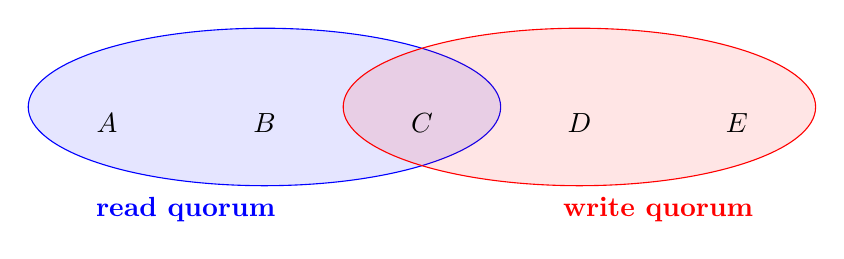
\begin{tikzpicture}
                \filldraw [blue,fill opacity=0.1] (2,2) circle [x radius=3,y radius=1];
                \filldraw [red,fill opacity=0.1] (6,2) circle [x radius=3,y radius=1];
                \node [blue] at (1,0.7) {\textbf{read quorum}};
                \node [red]  at (7,0.7) {\textbf{write quorum}};
                \node (A) at (0,2) {\storageSymbol}; \node [yshift=-0.2cm] at (A) {$A$};
                \node (B) at (2,2) {\storageSymbol}; \node [yshift=-0.2cm] at (B) {$B$};
                \node (C) at (4,2) {\storageSymbol}; \node [yshift=-0.2cm] at (C) {$C$};
                \node (D) at (6,2) {\storageSymbol}; \node [yshift=-0.2cm] at (D) {$D$};
                \node (E) at (8,2) {\storageSymbol}; \node [yshift=-0.2cm] at (E) {$E$};
            \end{tikzpicture}
        \end{center}
    \end{uncoverenv}
\end{frame}
\inlineslide{s:quorum}{}\label{l:quorum}

A system that requires $w$ acknowledgements for writes (i.e.\ a write quorum of size $w$) can continue processing updates as long as no more than $n-w$ replicas are unavailable, and a system that requires $r$ responses for reads can continue reading as long as no more than $n-r$ replicas are unavailable.
With majority quorums, this means that a system of three replicas can tolerate one replica being unavailable, a system of five replicas can tolerate two being unavailable, and so on.

In this quorum approach to replication, some updates may be missing from some replicas at any given moment: for example, on \autoref{l:quorum-example}, the $(t_1, v_1)$ update is missing from replica $A$, since that write request was dropped.
To bring replicas back in sync with each other, one approach is to rely on an anti-entropy process, as discussed on \autoref{l:reconcile}.

\begin{frame}
    \label{s:read-repair}
    \frametitle{Read repair}
    \begin{center}
        \begin{tikzpicture}
            \node [rectangle,fill=red!10,draw] (node1) at (0,5) {client};
            \node [rectangle,fill=red!10,draw] (node2) at (3,5) {\storageSymbol}; \node [yshift=-0.2cm] at (node2) {$A$};
            \node [rectangle,fill=red!10,draw] (node3) at (6,5) {\storageSymbol}; \node [yshift=-0.2cm] at (node3) {$B$};
            \node [rectangle,fill=red!10,draw] (node4) at (9,5) {\storageSymbol}; \node [yshift=-0.2cm] at (node4) {$C$};
            \draw (node1) -- (0,-0.3);
            \draw (node2) -- (3,-0.3);
            \draw (node3) -- (6,-0.3);
            \draw (node4) -- (9,-0.3);
            \draw<2-> [messageloss] (0,4.0) -- node [above,pos=0.2,sloped] {$\mathsf{get}(x)$} (8,3.2);
            \draw<2-> [bigarrow] (0,3.9) .. controls (1,3.8) and (1,3.5) .. (2,3.4) -- (6,3.0);
            \draw<2-> [bigarrow] (0,3.8) .. controls (1,3.7) and (1,3.1) .. (2,3.0) -- (3,2.9);
            \draw<3-> [bigarrow] (3,2.4) -- node [above,sloped] {$(t_0, v_0)$} (0,2.1);
            \draw<3-> [bigarrow] (6,2.3) -- node [above,sloped,near start] {$(t_1, v_1)$} (0,1.7);
            \draw<4-> [bigarrow] (0,0.8) -- node [above,sloped,pos=0.17] {$(t_1, \mathsf{set}(x,v_1))$} (9,-0.1);
            \draw<4-> [bigarrow] (0,0.7) .. controls (1,0.6) and (1,0.3) .. (2,0.2) -- (3,0.1);
        \end{tikzpicture}
    \end{center}%
    \uncover<3->{Update $(t_1, v_1)$ is more recent than $(t_0, v_0)$ since $t_0 < t_1$.}\\%
    \uncover<4->{Client helps \textbf{propagate} $(t_1, v_1)$ to other replicas.}
\end{frame}
\inlineslide{s:read-repair}{}\label{l:read-repair}

Another option is to get clients to help with the process of disseminating updates.
For example, on \autoref{l:read-repair}, the client reads $(t_1, v_1)$ from $B$, but it receives an older value $(t_0, v_0)$ from $A$, and no response from $C$.
Since the client now knows that the update $(t_1, v_1)$ needs to be propagated to $A$, it can send that update to $A$ (using the original timestamp $t_1$, since this is not a new update, only a retry of a previous update).
The client may also send the update to $C$, even though it does not know whether $C$ needs it (if it turns out that $C$ already has this update, only a small amount of network bandwidth is wasted).
This process is called \emph{read repair}.
The client can perform read repair on any read request it makes, regardless of whether it was the client that originally performed the update in question.

Databases that use this model of replication are often called \emph{Dynamo-style}, after Amazon's Dynamo database \citep{DeCandia:2007}, which popularised it.
However, the approach actually predates Dynamo \citep{Attiya:1995}.

\subsection{Replication using broadcast}\label{sec:broadcast-replication}

The quorum approach of \autoref{sec:quorums} essentially uses best-effort broadcast: a client broadcasts every read or write request to all of the replicas, but the protocol is unreliable (requests might be lost) and provides no ordering guarantees.

An alternative approach to replication is to use the broadcast protocols from \autoref{sec:broadcast}.
Let's first consider FIFO-total order broadcast, the strongest form of broadcast we have seen.

\begin{frame}
    \label{s:smr}
    \frametitle{State machine replication}
    So far we have used best-effort broadcast for replication.\\
    What about stronger broadcast models?\\[1em]\pause
    Total order broadcast: every node delivers the \textbf{same messages} in the \textbf{same order}\\[1em]\pause
    \textbf{State machine replication} (SMR):
    \begin{itemize}
        \item FIFO-total order broadcast every update to all replicas
        \item Replica delivers update message: apply it to own state\pause
        \item Applying an update is deterministic\pause
        \item Replica is a \textbf{state machine}: starts in fixed initial state,
            goes through same sequence of state transitions in the same order
            $\Longrightarrow$ all replicas end up in the same state
    \end{itemize}
\end{frame}
\inlineslide{s:smr}{}\label{l:smr}

Using FIFO-total order broadcast it is easy to build a replicated system: we broadcast every update request to the replicas, which update their state based on each message as it is delivered.
This is called \emph{state machine replication} (SMR), because a replica acts as a state machine whose inputs are message deliveries.
We only require that the update logic is \emph{deterministic}: any two replicas that are in the same state, and are given the same input, must end up in the same next state.
Even errors must be deterministic: if an update succeeds on one replica but fails on another, they would become inconsistent.

An excellent feature of SMR is that the logic for moving from one state to the next can be arbitrarily complex, as long as it is deterministic.
For example, an entire database transaction with arbitrary business logic can be executed, and this logic can depend both on the broadcast message and the current state of the database.
Some distributed database perform replication in this way, with each replica independently executing the same deterministic transaction code (this is known as \emph{active replication}).
This principle also underpins blockchains, cryptocurrencies, and distributed ledgers: the ``chain of blocks'' in a blockchain is nothing other than the sequence of messages delivered by a total order broadcast protocol (more on this in \autoref{sec:consensus}), and each replica deterministically executes the transactions described in those blocks to determine the state of the ledger (e.g.\ who owns which money).
A ``smart contract'' is just a deterministic program that a replica executes when a particular message is delivered.

\begin{frame}
    \label{s:smr2}
    \frametitle{State machine replication}
    \framebox{
        \begin{minipage}{10cm}
            \vspace*{3pt}
            \begin{algorithmic}
                \On{request to perform update $u$}
                    \State send $u$ via FIFO-total order broadcast
                \EndOn
                \State
                \On{delivering $u$ through FIFO-total order broadcast}
                    \State update state using arbitrary deterministic logic!
                \EndOn
            \end{algorithmic}
            \vspace*{3pt}
        \end{minipage}
    }\pause\vspace*{0.5em}
    Closely related ideas:
    \begin{itemize}
        \item Serializable transactions (execute in delivery order)\pause
        \item Blockchains, distributed ledgers, smart contracts\pause
    \end{itemize}
    Limitations:
    \begin{itemize}
        \item Cannot update state immediately, have to wait for delivery through broadcast\pause
        \item Need fault-tolerant total order broadcast: see next lecture
    \end{itemize}
\end{frame}
\inlineslide{s:smr2}{}\label{l:smr2}

The downsides of state machine replication are the limitations of total order broadcast.
As discussed in \autoref{sec:delivery-order}, when a node wants to broadcast a message through a total order broadcast, it cannot immediately deliver that message to itself.
For this reason, when using state machine replication, a replica that wants to update its state cannot do so immediately, but it has to go through the broadcast process, coordinate with other nodes, and wait for the update to be delivered back to itself.
The fault tolerance of state machine replication depends on the fault tolerance of the underlying total order broadcast, which we will discuss in \autoref{sec:consensus}.
Nevertheless, replication based on total order broadcast is widely used.

\begin{frame}
    \label{s:leader-database}
    \frametitle{Database leader replica}
    Leader database replica $L$ ensures total order broadcast
    \begin{center}
        \begin{tikzpicture}
            \node [rectangle,fill=red!10,draw] (node1) at (0,5) {client 1};
            \node [rectangle,fill=red!10,draw] (node2) at (3,5) {client 2};
            \node [rectangle,fill=red!10,draw] (node3) at (6,5) {\storageSymbol}; \node [yshift=-0.2cm] at (node3) {$L$};
            \node [rectangle,fill=red!10,draw] (node4) at (9,5) {\storageSymbol}; \node [yshift=-0.2cm] at (node4) {$F$};
            \draw (node1) -- (0,-0.3);
            \draw (node2) -- (3,-0.3);
            \draw (node3) -- (6,-0.3);
            \draw (node4) -- (9,-0.3);
            \node<2-> [rectangle,fill=white,draw,text depth=2.4cm] (T1) at (6,2.1) {$T_1$};
            \draw<2-> [bigarrow] (0,4.2) -- node [above,near start] {$T_1$} (T1.north west);
            \node<3-> [rectangle,fill=white,draw,text depth=0.6cm] (T2) at (6.4,2.0) {$T_2$};
            \draw<3-> [bigarrow] (3,2.9) -- node [above] {$T_2$} (T2.north west);
            \draw<4-> [bigarrow] (T2.south west) -- node [above,sloped] {ok} (3,1.1);
            \draw<4-> [bigarrow] (T2.south east) -- node [above,sloped] {commit} (9,1.1);
            \draw<5-> [bigarrow] (T1.south west) -- node [above,sloped,near end] {ok} (0,0);
            \draw<5-> [bigarrow] (T1.south east) -- node [below,sloped] {commit} (9,0.3);
        \end{tikzpicture}
    \end{center}%
    \uncover<4->{Follower $F$ applies transaction log in commit order}
\end{frame}
\inlineslide{s:leader-database}{}\label{l:leader-database}

Recall from \autoref{l:total-bcast-alg} that one way of implementing total order broadcast is to designate one node as the \emph{leader}, and to route all broadcast messages through it in order to impose a delivery order.
This principle is also widely used for database replication: many database systems designate one replica as \emph{leader}, \emph{primary}, or \emph{master}.
Any transactions that wish to modify the database must be executed on the leader replica.
As shown on \autoref{l:leader-database}, the leader may execute multiple transactions concurrently; however, it \emph{commits} those transactions in a total order.
When a transaction commits, the leader replica broadcasts the writes from that transaction to all the follower replicas, and the followers apply those writes in commit order.
This approach is known as \emph{passive replication} or \emph{primary-backup replication}, and we can see that it is equivalent to total order broadcast of transaction commit records.

So much on using total order broadcast for replication.
What about the other broadcast models from \autoref{sec:broadcast}~-- can we use them for replication too?
The answer is yes, as shown on \autoref{l:causal-replication}; however, more care is required to ensure that replicas remain consistent.
It is not sufficient to merely ensure that the state update is deterministic.

For example, we can use causal broadcast, which ensures the same delivery order across replicas when one update happened before another, but which may deliver concurrent updates in any order.
If we want to ensure that replicas end up in the same state, no matter in which order concurrent updates are delivered, we need to make those updates \emph{commutative}: that is, we have to ensure that the final result is the same, no matter in which order those updates are applied.
This can be done, and we will see some techniques for commutativity in \autoref{sec:eventual-consistency}.

\begin{frame}
    \label{s:causal-replication}
    \frametitle{Replication using causal (and weaker) broadcast}
    State machine replication uses (FIFO-)total order broadcast.\\
    Can we use weaker forms of broadcast too?\\[1em]\pause
    If replica state updates are \textbf{commutative}, replicas can process updates in different orders and still end up in the same state.\\[1em]
    Updates $f$ and $g$ are commutative if $f(g(x)) = g(f(x))$\\\pause
    \rowcolors[]{2}{}{blue!10}
    \renewcommand{\arraystretch}{1.3}
    \begin{tabular}{l|p{8cm}}
        \hline
        \textbf{broadcast} & \textbf{assumptions about state update function} \\\hline
        total order & deterministic (SMR) \pause\\
        causal & deterministic, concurrent updates commute \pause\\
        reliable & deterministic, all updates commute \pause\\
        best-effort & deterministic, commutative, idempotent,\newline tolerates message loss \\\hline
    \end{tabular}
\end{frame}
\inlineslide{s:causal-replication}{}\label{l:causal-replication}


% TODO reorder these sections as follows: first cover Raft (to follow on from SMR which we just covered); then atomic commit/2PC; then linearizability.

\section{Replica consistency}\label{sec:consistency}

\begin{frame}
    \begin{center}
        {\Large{\color{darkblue}{Replica consistency}}} \\[2em]
        \mydetails
    \end{center}
\end{frame}

We have seen how to perform replication using read/write quorums, and state machine replication using total order broadcast.
In this context we have said that we want replicas to have ``consistent copies of the same data'', without defining exactly what we mean with \emph{consistent}.

Unfortunately the word ``consistency'' means different things in different contexts.
In the context of transactions, the C in ACID stands for consistency that is a property of a state: that is, we can say that a database is in a consistent or inconsistent state, meaning that the state satisfies or violates certain invariants defined by the application.
On the other hand, in the context of replication, we have used ``consistency'' informally to refer to a relationship between replicas: we want one replica to be consistent with another replica.

Since there is no one true definition of consistency, we speak instead about a variety of \emph{consistency models}.
We have seen one particular example of a consistency model, namely read-after-write consistency (\autoref{l:read-after-write}), which restricts the values that a read operation may return when the same node previously writes to the same data item.
We will see more models in this lecture.

\begin{frame}
    \label{s:consistency}
    \frametitle{``Consistency''}
    A word that means many different things in different contexts!\pause
    \begin{itemize}
        \item \textbf{ACID}: a transaction transforms the database from one ``consistent'' state to another\\[0.5em]\pause
            Here, ``consistent'' = satisfying application-specific invariants\\[0.5em]
            e.g. ``every course with students enrolled must have at least one lecturer''\\[0.5em]\pause
        \item \textbf{Read-after-write consistency}\\[0.5em]\pause
        \item \textbf{Replication}: replica should be ``consistent'' with other replicas\\[0.5em]\pause
            ``consistent'' = in the same state? (when exactly?)\\[0.5em]
            ``consistent'' = read operations return same result?\\[0.5em]
        \item \textbf{Consistency model}: many to choose from
    \end{itemize}
\end{frame}
\inlineslide{s:consistency}{}\label{l:consistency}

\subsection{Two-phase commit}\label{sec:2pc}

Let's start with a consistency problem that arises when executing a \emph{distributed transaction}, i.e.\ a transaction that reads or writes data on multiple nodes.
The data on those nodes may be replicas of the same dataset, or different parts of a larger dataset; a distributed transaction applies in both cases.

Recall from the concurrent systems half of this course that a key property of a transaction is \emph{atomicity}.
When a transaction spans multiple nodes, we still want atomicity for the transaction as a whole: that is, either all nodes must commit the transaction and make its updates durable, or all nodes must abort the transaction and discard or roll back its updates.

\begin{frame}
    \label{s:atomic-commit}
    \frametitle{Distributed transactions}
    Recall \textbf{atomicity} in the context of ACID transactions:
    \begin{itemize}
        \item A transaction either \textbf{commits} or \textbf{aborts}\pause
        \item If it commits, its updates are durable
        \item If it aborts, it has no visible side-effects\pause
        \item ACID consistency (preserving invariants) relies on atomicity\pause\\[1em]
    \end{itemize}
    If the transaction updates data on multiple nodes, this implies:
    \begin{itemize}
        \item Either all nodes must commit, or all must abort\pause
        \item If any node crashes, all must abort\\[1em]
    \end{itemize}
    Ensuring this is the \textbf{atomic commitment} problem.
\end{frame}
\inlineslide{s:atomic-commit}{}\label{l:atomic-commit}

The most common algorithm to ensure atomic commitment across multiple nodes is the \emph{two-phase commit} (2PC) protocol \citep{Gray:1978}.
(Not to be confused with \emph{two-phase locking}: 2PL ensures serializable isolation for transactions, while 2PC ensures atomic commitment.
There is also a \emph{three-phase commit} protocol, but it assumes the unrealistic synchronous system model, so we won't discuss it here.)
The communication flow of 2PC is illustrated on \autoref{l:2pc}.

\begin{frame}
    \label{s:2pc}
    \frametitle{Two-phase commit (2PC)}
    \begin{center}
        \begin{tikzpicture}
            \node [rectangle,fill=red!10,draw] (node1) at (0,7.4) {client};
            \node [rectangle,fill=red!10,draw] (node2) at (3,7.4) {coordinator};
            \node [rectangle,fill=red!10,draw] (node3) at (6,7.4) {\storageSymbol}; \node [yshift=-0.2cm] at (node3) {$A$};
            \node [rectangle,fill=red!10,draw] (node4) at (9,7.4) {\storageSymbol}; \node [yshift=-0.2cm] at (node4) {$B$};
            \draw (node1) -- (0,0.3);
            \draw (node2) -- (3,0.3);
            \draw (node3) -- (6,0.3);
            \draw (node4) -- (9,0.3);
            \node<2-> [rectangle,fill=white,draw,text depth=4.6cm] (T1) at (6,3.3) {$T_1$};
            \node<2-> [rectangle,fill=white,draw,text depth=3.7cm] (T2) at (9,2.9) {$T_1$};
            \draw<2-> [bigarrow] (0,6.5) -- node [above,sloped,near start] {begin $T_1$} (T1.north west); % (5.65,5.9)
            \draw<2-> [bigarrow] (0,6.4) .. controls (1,6.3) and (1,5.8) .. (2,5.7) -- (T2.north west); % (8.65,5.0)
            \draw<3-> [blue,doublebigarrow] (0,4.5) -- node [above,blue,font=\footnotesize] {{\dots}usual transaction execution{\dots}} (5.65,4.5);
            \draw<3-> [blue,bigarrow] (6.35,4.5) -- (8.65,4.5);
            \draw<4-> [bigarrow] (0,3.9) -- node [above,sloped] {commit $T_1$} (3,3.6);
            \draw<5-> [bigarrow] (3,3.4) -- node [above,sloped,near start] {prepare} (8.65,2.8);
            \draw<5-> [bigarrow] (3,3.3) .. controls (4,3.2) and (4,3.0) .. (5,2.9) -- (5.65,2.83);
            \draw<6-> [bigarrow] (5.65,2.5) -- node [above,sloped] {ok} (3,2.2);
            \draw<6-> [bigarrow] (8.65,2.4) -- node [above,sloped,near start] {ok} (3,1.8);
            \draw<7-> [bigarrow] (3,1.3) -- node [above,sloped,near start] {commit} (T2.south west); % (8.65,0.7)
            \draw<7-> [bigarrow] (3,1.2) .. controls (4,1.1) and (4,0.9) .. (5,0.8) -- (T1.south west); % (5.65,0.73)
            \node<8-> [circle,fill=green,semitransparent,inner sep=5pt] (decision) at (3,1.5) {};
            \draw<8-> (decision.west) node [left,font=\scriptsize,text width=2.8cm,align=right,darkgreen] {decision whether to commit or abort};
        \end{tikzpicture}
    \end{center}
\end{frame}
\inlineslide{s:2pc}{}\label{l:2pc}

When using two-phase commit, a client first starts a regular single-node transaction on each replica that is participating in the transaction, and performs the usual reads and writes within those transactions.
When the client is ready to commit the transaction, it sends a commit request to the \emph{transaction coordinator}, a designated node that manages the 2PC protocol.
(In some systems, the coordinator is part of the client.)

The coordinator first sends a \emph{prepare} message to each replica participating in the transaction, and each replica replies with a message indicating whether it is able to commit the transaction (this is the first phase of the protocol).
The replicas do not actually commit the transaction yet, but they must ensure that they will definitely be able to commit the transaction in the second phase if instructed by the coordinator.
This means, in particular, that the replica must write all of the transaction's updates to disk and check any integrity constraints before replying \emph{ok} to the \emph{prepare} message, while continuing to hold any locks for the transaction.

The coordinator collects the responses, and decides whether or not to actually commit the transaction.
If all nodes reply \emph{ok}, the coordinator decides to commit; if any node wants to abort, or if any node fails to reply within some timeout, the coordinator decides to abort.
The coordinator then sends its decision to each of the replicas, who all commit or abort as instructed (this is the second phase).
If the decision was to commit, each replica is guaranteed to be able to commit its transaction because the previous \emph{prepare} request laid the groundwork.
If the decision was to abort, the replica rolls back the transaction.

\begin{frame}
    \label{s:2pc-coordinator}
    \frametitle{The coordinator in two-phase commit}
    What if the coordinator crashes?\pause
    \begin{itemize}
        \item Coordinator writes its decision to disk
        \item When it recovers, read decision from disk and send it to replicas
            (or abort if no decision was made before crash)\pause
        \item \textbf{Problem:} if coordinator crashes after prepare, but before broadcasting decision, other nodes do not know what it has decided\pause
        \item Replicas participating in transaction cannot commit or abort after responding ``ok'' to the \emph{prepare} request (otherwise we risk violating atomicity)\pause
        \item Algorithm is blocked until coordinator recovers
    \end{itemize}
\end{frame}
\inlineslide{s:2pc-coordinator}{}\label{l:2pc-coordinator}

The problem with two-phase commit is that the coordinator is a single point of failure.
Crashes of the coordinator can be tolerated by having the coordinator write its commit/abort decisions to stable storage, but even so, there may be transactions that have prepared but not yet committed/aborted at the time of the coordinator crash (called \emph{in-doubt transactions}).
Any in-doubt transactions must wait until the coordinator recovers to learn their fate; they cannot unilaterally decide to commit or abort, because that decision could end up being inconsistent with the coordinator and other nodes, which might violate atomicity.

Fortunately it is possible to avoid the single point of failure of the coordinator by using a total order broadcast protocol.
\autoref{l:paxos-commit1} shows a fault-tolerant two-phase commit algorithm based on Paxos Commit \citep{Gray:2006}.
The idea is that every node that is participating in the transaction uses total order broadcast to disseminate its vote on whether to commit or abort.
Moreover, if node $A$ suspects that node $B$ has failed (because no vote from $B$ was received within some timeout), then $A$ may try to vote to abort on behalf of $B$.
This introduces a race condition: if node $B$ is slow, it might be that node $B$ broadcasts its own vote to commit around the same time that node $A$ suspects $B$ to have failed and votes on $B$'s behalf.

These votes are delivered to each node by total order broadcast, and each recipient independently counts the votes.
In doing so, we count only the first vote from any given replica, and ignore any subsequent votes from the same replica.
Since total order broadcast guarantees the same delivery order on each node, all nodes will agree on whether the first delivered vote from a given replica was a commit vote or an abort vote, even in the case of a race condition between multiple nodes broadcasting contradictory votes for the same replica.

If a node observes that the first delivered vote from some replica is a vote to abort, then the transaction can immediately be aborted.
Otherwise a node must wait until it has delivered at least one vote from each replica.
Once these votes have been delivered, and none of the replicas vote to abort in their first delivered message, then the transaction can be committed.
Thanks to total order broadcast, all nodes are guaranteed to make the same decision on whether to abort or to commit, which preserves atomicity.

% TODO: visualise this algorithm graphically

\begin{frame}
    \label{s:paxos-commit1}
    \frametitle{Fault-tolerant two-phase commit (1/2)}
    \footnotesize
    \begin{algorithmic}
        \On{initialisation for transaction $T$}
            \State $\mathit{commitVotes}[T] := \{\};\; \mathit{replicas}[T] := \{\};\; \mathit{decided}[T] := \mathsf{false}$
        \EndOn
        \State
        \On{request to commit transaction $T$ with participating nodes $R$}
            \State \textbf{for each} $r \in R$ \textbf{do} send $(\mathsf{Prepare}, T, R)$ to $r$
        \EndOn
        \State
        \On{receiving $(\mathsf{Prepare}, T, R)$ at node $\mathit{replicaId}$}
            \State $\mathit{replicas}[T] := R$
            \State $\mathit{ok} = $ ``is transaction $T$ able to commit on this replica?''
            \State total order broadcast $(\mathsf{Vote}, T, \mathit{replicaId}, \mathit{ok})$ to $\mathit{replicas}[T]$
        \EndOn
        \State
        \On{a node suspects node $\mathit{replicaId}$ to have crashed}
            \For{each transaction $T$ in which $\mathit{replicaId}$ participated}
                \State total order broadcast $(\mathsf{Vote}, T, \mathit{replicaId}, \mathsf{false})$ to $\mathit{replicas}[T]$
            \EndFor
        \EndOn
    \end{algorithmic}
\end{frame}
\inlineslide{s:paxos-commit1}{}\label{l:paxos-commit1}

\begin{frame}
    \label{s:paxos-commit2}
    \frametitle{Fault-tolerant two-phase commit (2/2)}
    \footnotesize
    \begin{algorithmic}
        \On{delivering $(\mathsf{Vote}, T, \mathit{replicaId}, \mathit{ok})$ by total order broadcast}
            \If{$\mathit{replicaId} \notin \mathit{commitVotes}[T] \;\wedge\; \mathit{replicaId} \in \mathit{replicas}[T] \;\wedge$\\\hspace{60pt}$\neg\mathit{decided}[T]$}
                \If{$\mathit{ok} = \mathsf{true}$}
                    \State $\mathit{commitVotes}[T] := \mathit{commitVotes}[T] \cup \{\mathit{replicaId}\}$
                    \If{$\mathit{commitVotes}[T] = \mathit{replicas}[T]$}
                        \State $\mathit{decided}[T] := \mathsf{true}$
                        \State commit transaction $T$ at this node
                    \EndIf
                \Else
                    \State $\mathit{decided}[T] := \mathsf{true}$
                    \State abort transaction $T$ at this node
                \EndIf
            \EndIf
        \EndOn
    \end{algorithmic}
\end{frame}
\inlineslide{s:paxos-commit2}{}\label{l:paxos-commit2}

\subsection{Linearizability}\label{sec:linearizability}

An atomic commitment protocol is a way of preserving consistency across multiple replicas in the face of faults, by ensuring that all participants of a transaction either commit or abort.
However, when there are multiple nodes concurrently reading and modifying some shared data concurrently, ensuring the same commit or abort outcome for all nodes is not sufficient.
We also have to reason about the interaction that arises from concurrent activity.

In this section we will introduce one particular consistency model for concurrent system that is called \emph{linearizability}.
We will discuss linearizability informally; if you are interested in the details, \cite{Herlihy:1990} give a formal definition.
People sometimes say \emph{strong consistency} when referring to linearizability, but the concept of ``strong consistency'' is rather vague and imprecise.
We will stick to the term \emph{linearizability}, which has a precisely defined meaning.
% TODO: mention that a linearizable register is also known as an atomic register?

An informal definition of linearizability appears on \autoref{l:linearizability}.
Over the following slides we will clarify what this means through examples.
The concept of linearizability can be applied to any type of object, but it is most commonly used in the context of a register.
A linearizable register is sometimes also known as an \emph{atomic register}.

Linearizability is a useful concept not only in distributed systems, but also in the context of shared-memory concurrency on a single machine.
Interestingly, on a computer with multiple CPU cores (pretty much all servers, laptops and smartphones nowadays), memory access is not linearizable by default!
This is because each CPU core has its own caches, and an update made by one core is not immediately reflected in another core's cache.
Thus, even a single computer starts behaving a bit like a replicated system.
The \href{\multicore}{L304 unit in Part~III} goes into detail of multicore memory behaviour.
% TODO: Introduction to Computer Architecture discusses multicore cache coherence and barriers https://www.cl.cam.ac.uk/teaching/2122/IntComArch/
% This course runs in part IB in the first 5 weeks of Michaelmas term, just before this lecture

Don't confuse linearizability with serializability, even though both words seem to mean something like ``can be arranged into a sequential order''.
Serializability means that transactions have the same effect as if they had been executed in \emph{some} serial order, but it does not define what that order should be.
Linearizability defines the values that operations must return, depending on the concurrency and relative ordering of those operations.
It is possible for a system to provide both serializability and linearizability: the combination of the two is called \emph{strict serializability} or \emph{one-copy serializability}.

\begin{frame}
    \label{s:linearizability}
    \frametitle{Linearizability}
    Multiple nodes concurrently accessing replicated data.\\
    How do we define ``consistency'' here?\\[1em]\pause
    The strongest option: \textbf{linearizability}\pause
    \begin{itemize}
        \item Informally: every operation takes effect \textbf{atomically} sometime after it started and before it finished\pause
        \item All operations behave as if executed on a \textbf{single copy} of the data (even if there are in fact multiple replicas)\pause
        \item Consequence: every operation returns an ``up-to-date'' value, a.k.a.\ ``strong consistency''\pause
        \item Not just in distributed systems, also in shared-memory concurrency (memory on multi-core CPUs is not linearizable by default!)\pause
    \end{itemize}
    Note: linearizability $\neq$ serializability!
\end{frame}
\inlineslide{s:linearizability}{}\label{l:linearizability}

The main purpose of linearizability is to guarantee that nodes observe the system in an ``up-to-date'' state; that is, they do not read \emph{stale} (outdated) values.
We have previously seen this concept of reading an ``up-to-date'' value in the context of read-after-write consistency (\autoref{l:read-after-write}).
However, while read-after-write consistency defines only a consistency model for reads and writes made by the same node, linearizability generalises this idea to operations made concurrently by different nodes.

From the point of view of a client, every operation takes some amount of time.
We say that an operation \emph{starts} at the moment when it is requested by the application, and it \emph{finishes} when the operation result is returned to the application.
Between the start and finish, various network communication steps may happen; for example, if quorums are used, an operation can finish when the client has received responses from a quorum of replicas.

Let's consider a register supporting $\mathsf{get}$/$\mathsf{set}$ operations, and see what it means for it to be linearizable.
On \autoref{l:read-after-write-2} and the following slides we represent the client's view of an operation as a rectangle covering the period of time from the start to finish of an operation.
Inside the rectangle we write the effect of the operation: $\mathsf{set}(x,v)$ means updating the register $x$ to have the value $v$, and $\mathsf{get}(x) \rightarrow v$ means a read of $x$ that returns the value $v$.

\begin{frame}
    \label{s:read-after-write-2}
    \frametitle{Read-after-write consistency revisited}
    \begin{center}
        \begin{tikzpicture}
            \node [rectangle,fill=red!10,draw] (node1) at (0,5.7) {client};
            \node [rectangle,fill=red!10,draw] (node2) at (3,5.7) {\storageSymbol}; \node [yshift=-0.2cm] at (node2) {$A$};
            \node [rectangle,fill=red!10,draw] (node3) at (6,5.7) {\storageSymbol}; \node [yshift=-0.2cm] at (node3) {$B$};
            \node [rectangle,fill=red!10,draw] (node4) at (9,5.7) {\storageSymbol}; \node [yshift=-0.2cm] at (node4) {$C$};
            \draw (node1) -- (0,-1.5);
            \draw (node2) -- (3,-1.5);
            \draw (node3) -- (6,-1.5);
            \draw (node4) -- (9,-1.5);
            \node<2-> [op,text width=2.2cm] (op1) at (0,3.4) {$\mathsf{set}(x,v_1)$};
            \draw<2-> [bigarrow] (0.3,4.5) -- node [above,pos=0.15,sloped] {$(t_1, \mathsf{set}(x,v_1))$} (9,3.6);
            \draw<2-> [bigarrow] (0.3,4.4) .. controls (1,4.33) and (1,4.0) .. (2,3.9) -- (6,3.5);
            \draw<2-> [messageloss] (0.3,4.3) .. controls (1,4.23) and (1,3.6) .. (2,3.5) -- (2.5,3.45);
            \draw<3-> [bigarrow] (6,3.2) -- node [above,sloped,pos=0.30] {ok} (0.3,2.6);
            \draw<3-> [bigarrow] (9,3.1) -- node [above,sloped,pos=0.17] {ok} (0.3,2.2);
            \node<4-> [op,text width=2.0cm] (op2) at (0,0.3) {$\mathsf{get}(x) \rightarrow v_1$};
            \draw<4-> [messageloss] (0.3,1.4) -- node [above,pos=0.2,sloped] {$\mathsf{get}(x)$} (8,0.6);
            \draw<4-> [bigarrow] (0.3,1.3) .. controls (1,1.23) and (1,0.9) .. (2,0.8) -- (6,0.4);
            \draw<4-> [bigarrow] (0.3,1.2) .. controls (1,1.13) and (1,0.5) .. (2,0.4) -- (3,0.3);
            \draw<5-> [bigarrow] (3,0.0) -- node [above,sloped,pos=0.5,yshift=-0.1cm] {$(t_0, v_0)$} (0.3,-0.3);
            \draw<5-> [bigarrow] (6,-0.1) -- node [above,sloped,near start,yshift=-0.1cm] {$(t_1, v_1)$} (0.3,-0.7);
        \end{tikzpicture}
    \end{center}%
\end{frame}
\inlineslide{s:read-after-write-2}{}\label{l:read-after-write-2}

Linearizability is independent of the system implementation and communication protocols: all that matters is the timing of each operation's start and finish, and the outcome of the operation.
We can therefore leave out all of the replicas and message-sending arrows, and look at the system's behaviour only from the client's point of view.

The key thing that linearizability cares about is whether one operation finished before another operation started, regardless of the nodes on which they took place.
On \autoref{l:read-after-write-3}, the two $\mathsf{get}$ operations both start after the $\mathsf{set}$ operation has finished, and therefore we expect the $\mathsf{get}$ operations to return the value $v_1$ written by $\mathsf{set}$.

\begin{frame}
    \label{s:read-after-write-3}
    \frametitle{From the client's point of view}
    \begin{columns}
        \begin{column}{0.4\textwidth}
            \begin{tikzpicture}
                \node<1-> [rectangle,fill=red!10,draw] (node1) at (0,7) {client 1};
                \node<4-> [rectangle,fill=red!10,draw] (node2) at (3,7) {client 2};
                \draw<1-> (node1) -- (0,0);
                \draw<4-> (node2) -- (3,0);
                \node<1-> [op,text width=2.2cm] (op1) at (0,4.9) {$\mathsf{set}(x,v_1)$};
                \draw<2-> [bigarrow] (op1.north west) -- node [at end,right] {?} +(0.9,-0.3);
                \draw<2-> [revbigarrow] (op1.north east) -- node [at end,right] {?} +(0.9,0.3);
                \node<1-3> [op,text width=2.0cm] (op2) at (0,1.8) {$\mathsf{get}(x) \rightarrow v_1$};
                \draw<2-3> [bigarrow] (op2.north west) -- +(0.9,-0.3);
                \draw<2-3> [revbigarrow] (op2.north east) -- +(0.9,0.3);
                \node<2-> at (1.5,2.6) {?};
                \node<2-> at (1.5,1.0) {?};
                \node<4-> [op,text width=2.0cm] (op3) at (3,1.8) {$\mathsf{get}(x) \rightarrow v_1$};
                \draw<4-> [bigarrow] (op3.south west) -- +(-0.9,-0.3);
                \draw<4-> [revbigarrow] (op3.south east) -- +(-0.9,0.3);
                \draw<3> (0.1,3.6) edge [-{Stealth},red,thick,densely dashed,out=330,in=50] node [pos=0.7,right,red,font=\scriptsize] {real time} (0.1,3.0);
                \draw<4-> (0.1,3.6) edge [-{Stealth},red,thick,densely dashed,out=330,in=150] node [above,red,font=\scriptsize] {real time} (2.9,3.0);
            \end{tikzpicture}
        \end{column}
        \begin{column}{0.6\textwidth}
            \begin{itemize}
                \item<1-> Focus on client-observable behaviour: when and what an operation returns
                \item<2-> Ignore how the replication system is implemented internally
                \item<3-> Did operation $A$ finish before operation $B$ started?
                \item<4-> Even if the operations are on different nodes?
                \item<5-> \textbf{This is not happens-before}:\\
                    we want client 2 to read value written by client 1, even if the clients have not communicated!
            \end{itemize}
        \end{column}
    \end{columns}
\end{frame}
\inlineslide{s:read-after-write-3}{}\label{l:read-after-write-3}

On the other hand, on \autoref{l:overlapping}, the $\mathsf{get}$ and $\mathsf{set}$ operation overlap in time: in this case we don't necessarily know in which order the operations take effect.
$\mathsf{get}$ may return either the value $v_1$ written by $\mathsf{set}$, or $x$'s previous value $v_0$, and either result is acceptable.

Note that ``operation A finished before operation B started'' is not the same as ``A happened before B''.
The happens-before relation (\autoref{sec:causality}) is defined in terms of messages sent and received; it is possible to have two operations that do not overlap in time, but are still concurrent according to the happens-before relation, because no communication has occurred between those operations.
On the other hand, linearizability is defined in terms of \emph{real time}: that is, a hypothetical global observer who can instantaneously see the state of all nodes (or, a perfectly synchronised clock on each node) determines the start and finish times of each operation.
In reality, such a global observer or perfectly synchronised clock does not exist in a system with variable network latency, but we can nevertheless define linearizability in terms of such a hypothetical observer.
This has the advantage that if we prove a system to be linearizable, we can be sure that its consistency guarantees hold regardless of whether some communication has taken place or not.

\begin{frame}
    \label{s:overlapping}
    \frametitle{Operations overlapping in time}
    \begin{columns}
        \begin{column}{0.5\textwidth}
            \begin{tikzpicture}
                \node [rectangle,fill=red!10,draw] (node1) at (0,7) {client 1};
                \node [rectangle,fill=red!10,draw] (node2) at (2,7) {\storageSymbol};
                \node [rectangle,fill=red!10,draw] (node3) at (4,7) {client 2};
                \draw (node1) -- (0,0);
                \draw (node2) -- (2,0);
                \draw (node3) -- (4,0);
                \node [op,text width=2.5cm] (op1) at (0,3.5) {$\mathsf{set}(x,v_1)$};
                \node<1-2> [op,text width=2.5cm] (op2) at (4,2.8) {$\mathsf{get}(x) \rightarrow v_1$};
                \node<3-|handout:0> [op,text width=2.5cm] (op3) at (4,2.8) {$\mathsf{get}(x) \rightarrow v_0$};
                \node [inner sep=0] (atomic1L) at (1.7,3.5) {}; \node [inner sep=0] (atomic1R) at (2.3,3.5) {};
                \node [inner sep=0] (atomic2L) at (1.7,2.9) {}; \node [inner sep=0] (atomic2R) at (2.3,2.9) {};
                \draw [blue,line width=4pt] (atomic1L) -- (atomic1R);
                \draw [blue,line width=4pt] (atomic2L) -- (atomic2R);
                \draw<1-2> [bigarrow] (op1.north west) -- (atomic1L);
                \draw<1-2> [bigarrow] (atomic1L) -- (op1.north east);
                \draw<1-2> [bigarrow] (op2.south west) -- (atomic2R);
                \draw<1-2> [bigarrow] (atomic2R) -- (op2.south east);
                \draw<3-|handout:0> [bigarrow] (op1.north west) -- (atomic2L);
                \draw<3-|handout:0> [bigarrow] (atomic2L) -- (op1.north east);
                \draw<3-|handout:0> [bigarrow] (op2.south west) -- (atomic1R);
                \draw<3-|handout:0> [bigarrow] (atomic1R) -- (op2.south east);
            \end{tikzpicture}
        \end{column}
        \begin{column}{0.5\textwidth}
            \begin{itemize}
                \item<1-> Client 2's get operation overlaps in time with client 1's set operation
                \item<2-> Maybe the set operation takes effect first?
                \item<3-> Just as likely, the get operation may be executed first
                \item<4-> Either outcome is fine in this case
            \end{itemize}
        \end{column}
    \end{columns}
\end{frame}
\inlineslide{s:overlapping}{}\label{l:overlapping}

Linearizability is not only about the relationship of a $\mathsf{get}$ operation to a prior $\mathsf{set}$ operation, but it can also relate one $\mathsf{get}$ operation to another.
\autoref{l:non-linearizable} shows an example of a system that uses quorum reads and writes, but is nevertheless non-linearizable.
Here, client 1 sets $x$ to $v_1$, and due to a quirk of the network the update to replica $A$ happens quickly, while the updates to replicas $B$ and $C$ are delayed.
Client 2 reads from a quorum of $\{A,B\}$, receives responses $\{v_0,v_1\}$, and determines $v_1$ to be the newer value based on the attached timestamp.
After client 2's read has finished, client 3 starts a read from a quorum of $\{B,C\}$, receives $v_0$ from both replicas, and returns $v_0$ (since it is not aware of $v_1$).

Thus, client 3 observes an older value than client 2, even though the real-time order of operations would require client 3's read to return a value that is no older than client 2's result.
This behaviour is not allowed in a linearizable system.

\begin{frame}
    \label{s:non-linearizable}
    \frametitle{Not linearizable, despite quorum reads/writes}
    \begin{tikzpicture}
        \node [rectangle,fill=red!10,draw] (node1) at (0,5.9) {client 1};
        \node [rectangle,fill=red!10,draw] (node2) at (2,5.9) {\storageSymbol}; \node [yshift=-0.2cm] at (node2) {$A$};
        \node [rectangle,fill=red!10,draw] (node3) at (4,5.9) {\storageSymbol}; \node [yshift=-0.2cm] at (node3) {$B$};
        \node [rectangle,fill=red!10,draw] (node4) at (6,5.9) {\storageSymbol}; \node [yshift=-0.2cm] at (node4) {$C$};
        \node [rectangle,fill=red!10,draw] (node5) at (8,5.9) {client 2};
        \node [rectangle,fill=red!10,draw] (node6) at (10,5.9) {client 3};
        \draw (node1) -- (0,-1);
        \draw (node2) -- (2,-1);
        \draw (node3) -- (4,-1);
        \draw (node4) -- (6,-1);
        \draw (node5) -- (8,-1);
        \draw (node6) -- (10,-1);
        \node<2-> [op,text width=5.2cm] at (0,2.0) {$\mathsf{set}(x,v_1)$};
        \draw<2-> [bigarrow] (0.3,4.7) -- node [above,sloped,font=\scriptsize,pos=0.4] {$(t_1, \mathsf{set}(x,v_1))$} (2,4.5);
        \draw<7-> [bigarrow] (0.3,4.6) .. controls (1.1,4.53) and (1.1,1.1) .. (2,1.0) -- (4,0.8);
        \draw<7-> [bigarrow] (0.3,4.5) .. controls (1,4.43) and (1,0.7) .. (2,0.6) -- (6,0.2);
        \draw<2-> [bigarrow] (2,4.2) -- node [above,sloped,font=\footnotesize] {ok} (0.3,4.0);
        \draw<8-> [bigarrow] (4,0.0) -- node [above,sloped,font=\footnotesize,near start] {ok} (0.3,-0.4);
        \draw<8-> [bigarrow] (6,-0.1) -- node [above,sloped,font=\footnotesize,pos=0.17] {ok} (0.3,-0.7);
        \node<3-> [op,text width=1.9cm] at (8,3.6) {$\mathsf{get}(x) \rightarrow v_1$};
        \draw<3-> [bigarrow] (7.7,4.5) -- node [above,pos=0.15,sloped,font=\footnotesize] {$\mathsf{get}(x)$} (2,3.9);
        \draw<3-> [bigarrow] (7.7,4.4) .. controls (7,4.33) and (7,4.1) .. (6,4.0) -- (4,3.8);
        \draw<4-> [bigarrow] (2,3.6) -- node [above,sloped,pos=0.19,font=\footnotesize,yshift=-0.1cm] {$(t_1, v_1)$} (7.7,3.0);
        \draw<4-> [bigarrow] (4,3.0) -- node [below,sloped,pos=0.25,font=\footnotesize,yshift=0.1cm] {$(t_0, v_0)$} (7.7,2.6);
        \node<5-> [op,text width=1.9cm] at (10,1.0) {$\mathsf{get}(x) \rightarrow v_0$};
        \draw<5-> [bigarrow] (9.7,2.0) -- node [above,pos=0.15,sloped,font=\footnotesize] {$\mathsf{get}(x)$} (4,1.4);
        \draw<5-> [bigarrow] (9.7,1.9) .. controls (9,1.83) and (9,1.6) .. (8,1.5) -- (6,1.3);
        \draw<6-> [bigarrow] (4,1.1) -- node [above,sloped,pos=0.19,font=\footnotesize,yshift=-0.1cm] {$(t_0, v_0)$} (9.7,0.5);
        \draw<6-> [bigarrow] (6,0.5) -- node [below,sloped,pos=0.25,font=\footnotesize,yshift=0.1cm] {$(t_0, v_0)$} (9.7,0.1);
    \end{tikzpicture}
\end{frame}
\inlineslide{s:non-linearizable}{}\label{l:non-linearizable}

\begin{frame}
    \label{s:non-linearizable-2}
    \frametitle{Not linearizable, despite quorum reads/writes}
    \begin{tikzpicture}
        \node [rectangle,fill=red!10,draw] (node1) at (0,5.7) {client 1};
        \node [rectangle,fill=red!10,draw] (node5) at (8,5.7) {client 2};
        \node [rectangle,fill=red!10,draw] (node6) at (10,5.7) {client 3};
        \draw (node1) -- (0,-1);
        \draw (node5) -- (8,-1);
        \draw (node6) -- (10,-1);
        \node [op,text width=5.2cm] at (0,2.0) {$\mathsf{set}(x,v_1)$};
        \node [op,text width=1.9cm] at (8,3.6) {$\mathsf{get}(x) \rightarrow v_1$};
        \node [op,text width=1.9cm] at (10,1.0) {$\mathsf{get}(x) \rightarrow v_0$};
        \draw<2-> (8.1,2.4) edge [-{Stealth},red,thick,densely dashed,out=340,in=160] node [above,red,font=\scriptsize] {real time} (9.9,2.1);
        \node<3-> at (4,2.5) {\begin{minipage}{6cm}
            \begin{itemize}
                \item Client 2's operation finishes before client 3's operation starts
                \item Linearizability therefore requires client 3's operation to observe a state no older than client 2's operation
                \item This example violates linearizability because $v_0$ is older than $v_1$
            \end{itemize}
        \end{minipage}};
    \end{tikzpicture}
\end{frame}
\inlineslide{s:non-linearizable-2}{}\label{l:non-linearizable-2}

Fortunately, it is possible to make $\mathsf{get}$ and $\mathsf{set}$ operations linearizable using quorum reads and writes.
First, for simplicity, assume that $\mathsf{set}$ operations are only performed by one designated node (we will remove this assumption later).
In this model, $\mathsf{set}$ operations don't change: as before, they send the update to all replicas, and wait for acknowledgement from a quorum of replicas.

For $\mathsf{get}$ operations, another step is required, as shown on \autoref{l:non-linearizable-3}.
A client must first send the $\mathsf{get}$ request to replicas, and wait for responses from a quorum.
If some responses include a more recent value than other responses, as indicated by their timestamps, then the client must write back the most recent value to all replicas that did not already respond with the most recent value, like in read repair (\autoref{l:read-repair}).
The $\mathsf{get}$ operation finishes only after the client is sure that the most recent value is stored on a quorum of replicas: that is, after a quorum of replicas either responded $\mathsf{ok}$ to the read repair, or replied with the most recent value in the first place.

This approach is known as the \emph{ABD algorithm}, after its authors Attiya, Bar-Noy, and Dolev \citep{Attiya:1995}.
It ensures linearizable reads and writes, because whenever a $\mathsf{get}$ and $\mathsf{set}$ operation finishes, we know that the value read or written is present on a quorum of replicas, and therefore any subsequent quorum read is guaranteed to observe that value (or a later value).

\supervision{
    Give pseudocode for the ABD algorithm.
}{
    Each replica executes the following:
    \begin{algorithmic}
        \On{initialisation}
            \State $\mathit{values} := \{\}$
        \EndOn
        \State
        \On{receiving $(\mathsf{get}, k)$ from a client}
            \State \textbf{send} $\{(t,v) \mid (t,k,v) \in \mathit{values}\}$ as response
        \EndOn
        \State
        \On{receiving $(\mathsf{set}, t, k, v)$ from a client}
            \If{$\nexists t', v'.\; (t', k, v') \in \mathit{values} \wedge t < t'$}
                \State $\mathit{values} := \{(t',k',v') \in \mathit{values} \mid k' \neq k\} \,\cup\, \{(t,k,v)\}$
            \EndIf
            \State \textbf{send} $\mathsf{ok}$ as response
        \EndOn
        \State
    \end{algorithmic}

    % TODO: This does not handle the case when the replica returns an empty set because it has no value for the given key
    \noindent Each client executes the following:
    \begin{algorithmic}
        \On{initialisation}
            \State $\mathit{writes} := 0$
        \EndOn
        \State
        \On{request to read value for key $k$}
            \State \textbf{send} $(\mathsf{get}, k)$ to each replica in $\mathit{replicas}$
            \State $\mathit{responses} := \{\}$
            \While{$|\mathit{responses}| < \left\lceil \frac{|\mathit{replicas}| + 1}{2} \right\rceil$}
                \State \textbf{receive response} $(t,v)$ from replica $i$
                \State $\mathit{responses} := \mathit{responses} \,\cup\, \{(i,t,v)\}$
            \EndWhile
            \State $\mathit{maxt} := \max(\{t \mid \exists i,v.\; (i,t,v) \in \mathit{responses}\})$
            \State $\mathit{maxv} := \text{the unique value } v \text{ such that } \exists i.\; (i,\mathit{maxt},v) \in \mathit{responses}$
            \State \textbf{send} $(\mathsf{set}, \mathit{maxt}, k, \mathit{maxv})$ to each replica in $\{i \in \mathit{replicas} \mid (i, \mathit{maxt}, \mathit{maxv}) \notin \mathit{responses}\}$
            \While{$|\{i \mid (i, \mathit{maxt}, \mathit{maxv}) \in \mathit{responses}\}| < \left\lceil \frac{|\mathit{replicas}| + 1}{2} \right\rceil$}
                \State \textbf{receive response} $\mathsf{ok}$ from replica $i$
                \State $\mathit{responses} := \mathit{responses} \,\cup\, \{(i, \mathit{maxt}, \mathit{maxv})\}$
            \EndWhile
            \State \textbf{return} $\mathit{maxv}$
        \EndOn
        \State
        \On{request to set key $k$ to value $v$} \Comment{NOTE: only one designated node may perform writes}
            \State $\mathit{writes} := \mathit{writes} + 1$
            \State \textbf{send} $(\mathsf{set}, \mathit{writes}, k, v)$ to each replica in $\mathit{replicas}$
            \State $\mathit{responses} := \{\}$
            \While{$|\mathit{responses}| < \left\lceil \frac{|\mathit{replicas}| + 1}{2} \right\rceil$}
                \State \textbf{receive response} $\mathsf{ok}$ from replica $i$
                \State $\mathit{responses} := \mathit{responses} \,\cup\, \{i\}$
            \EndWhile
        \EndOn
    \end{algorithmic}
}

\begin{frame}
    \label{s:non-linearizable-3}
    \frametitle{ABD: Making quorum reads/writes linearizable}
    \begin{tikzpicture}
        \node [rectangle,fill=red!10,draw] (node1) at (0,5.9) {client 1};
        \node [rectangle,fill=red!10,draw] (node2) at (2,5.9) {\storageSymbol}; \node [yshift=-0.2cm] at (node2) {$A$};
        \node [rectangle,fill=red!10,draw] (node3) at (4,5.9) {\storageSymbol}; \node [yshift=-0.2cm] at (node3) {$B$};
        \node [rectangle,fill=red!10,draw] (node4) at (6,5.9) {\storageSymbol}; \node [yshift=-0.2cm] at (node4) {$C$};
        \node [rectangle,fill=red!10,draw] (node5) at (8,5.9) {client 2};
        \node [rectangle,fill=red!10,draw] (node6) at (10,5.9) {client 3};
        \draw (node1) -- (0,-1);
        \draw (node2) -- (2,-1);
        \draw (node3) -- (4,-1);
        \draw (node4) -- (6,-1);
        \draw (node5) -- (8,-1);
        \draw (node6) -- (10,-1);
        \node<1-> [op,text width=5.2cm] (op1) at (0,2.0) {$\mathsf{set}(x,v_1)$};
        \draw<1-> [bigarrow] (0.3,4.7) -- node [above,sloped,font=\scriptsize,pos=0.4] {$(t_1, \mathsf{set}(x,v_1))$} (2,4.5);
        \draw<1-> [bigarrow] (0.3,4.6) .. controls (1.1,4.53) and (1.1,1.1) .. (2,1.0) -- (4,0.8);
        \draw<1-> [bigarrow] (0.3,4.5) .. controls (1,4.43) and (1,0.7) .. (2,0.6) -- (6,0.2);
        \draw<1-> [bigarrow] (2,4.2) -- node [above,sloped,font=\footnotesize] {ok} (0.3,4.0);
        \draw<6-> [bigarrow] (4,0.0) -- node [above,sloped,font=\footnotesize,near start] {ok} (0.3,-0.4);
        \draw<6-> [bigarrow] (6,-0.1) -- node [above,sloped,font=\footnotesize,pos=0.17] {ok} (0.3,-0.7);
        \node<1-> [op,text width=3.6cm] (op2) at (8,2.6) {$\mathsf{get}(x) \rightarrow v_1$};
        \draw<2-> [bigarrow] (7.7,4.5) -- node [above,pos=0.15,sloped,font=\footnotesize] {$\mathsf{get}(x)$} (2,3.9);
        \draw<2-> [bigarrow] (7.7,4.4) .. controls (7,4.33) and (7,4.1) .. (6,4.0) -- (4,3.8);
        \draw<3-> [bigarrow] (2,3.6) -- node [above,sloped,pos=0.19,font=\footnotesize,yshift=-0.1cm] {$(t_1, v_1)$} (7.7,3.0);
        \draw<3-> [bigarrow] (4,3.0) -- node [below,sloped,pos=0.25,font=\footnotesize,yshift=0.1cm] {$(t_0, v_0)$} (7.7,2.6);
        \draw<4-> [bigarrow] (7.7,2.1) -- node [above,pos=0.32,sloped,font=\footnotesize,yshift=-0.1cm] {$(t_1, \mathsf{set}(x,v_1))$} (4,1.7);
        \draw<4-> [bigarrow] (7.7,2.0) .. controls (7,1.93) and (7,1.7) .. (6,1.6);
        \draw<5-> [bigarrow] (6,1.27) -- node [above,sloped,font=\footnotesize] {ok} (7.7,1.1);
        \draw<5-> [bigarrow] (4,1.1) -- node [above,sloped,near start,font=\footnotesize] {ok} (7.7,0.7);
        \node<1-> [op,text width=1.9cm] (op3) at (10,1.0) {$\mathsf{get}(x) \rightarrow v_1$};
        \draw<1-> [bigarrow] (op3.south west) -- node [at end,below,yshift=-0.2cm] {\dots} +(-0.7,-0.1);
        \draw<1-> [revbigarrow] (op3.south east) -- node [at end,above] {\dots} +(-0.7,0.1);
    \end{tikzpicture}
\end{frame}
\inlineslide{s:non-linearizable-3}{}\label{l:non-linearizable-3}

To generalise the ABD algorithm to a setting where multiple nodes may perform $\mathsf{set}$ operations, we need to ensure timestamps reflect the real-time ordering of operations.
Say operation $\mathsf{set}(x, v_1)$ has a timestamp of $t_1$, operation $\mathsf{set}(x, v_2)$ has a timestamp of $t_2$, and the first operation finishes before the second operation starts: then we must ensure that $t_1 < t_2$.

We can do this by having each $\mathsf{set}$ operation first request the latest timestamp from each replica and waiting for responses from a quorum (like in a $\mathsf{get}$ operation).
The logical timestamp for the $\mathsf{set}$ operation is then one plus the maximum timestamp received from the quorum.
Since the quorum is guaranteed to contain at least one replica that has observed any $\mathsf{set}$ operation that has completed, we get the required ordering of timestamps.

However, if two different clients are concurrently performing $\mathsf{set}$ operations, this approach could result in two different operations having the same timestamp.
To tell them apart, we can give each client a unique ID, and incorporate that ID into the timestamps generated by that client.
When a $\mathsf{get}$ operation encounters responses with the same timestamp, but different client IDs, it can use a total ordering on client IDs to determine which one is the ``winner'' (similarly to the Lamport timestamp definition we saw on \autoref{l:lamport-definition} to \ref{l:lamport-example}).
This algorithm ensures linearizable $\mathsf{get}$ and $\mathsf{set}$ operations for any number of nodes \citep{Cachin:2011,Lynch:1997}.

% TODO: add a slide explaining single-writer ABD and the multi-writer generalisation, including logical timestamps construction.
% Multi-writer generalisation first appears in \cite{Lynch:1997}

\begin{frame}
    \label{s:cas-1}
    \frametitle{Linearizability for different operations}
    This ensures linearizability of $\mathsf{get}$ (quorum read) and\\$\mathsf{set}$ (\textbf{blind write} to quorum)\pause
    \begin{itemize}
        \item When an operation finishes, the value read/written is stored on a quorum of replicas
        \item Every subsequent quorum operation will see that value\pause
        \item Multiple concurrent writes may overwrite each other\\[1em]\pause
    \end{itemize}
    What about an atomic \textbf{compare-and-swap} operation?
    \begin{itemize}
        \item $\mathsf{CAS}(x, \mathit{oldValue}, \mathit{newValue})$ sets $x$ to $\mathit{newValue}$
            iff current value of $x$ is $\mathit{oldValue}$
        \item Previously discussed in shared-memory concurrency\pause
        \item Can we implement \textbf{linearizable} compare-and-swap in a distributed system?\pause
        \item \textbf{Yes:} total order broadcast to the rescue again!
    \end{itemize}
\end{frame}
\inlineslide{s:cas-1}{}\label{l:cas-1}

The $\mathsf{set}$ operation for which the ABD algorithm ensures linearizability is a so-called \emph{blind write} (unconditional write): it simply overwrites the value of the register, regardless of its previous value.
If multiple clients concurrently write to the same item, it uses a last-writer-wins conflict resolution policy (\autoref{l:concurrent-writes}), i.e.\ one of those writes will end up as the ``winner'' and the other values will silently be discarded.

In some applications, we want to be more careful and overwrite a value only if it has not been concurrently modified by another node.
This can be achieved with an \emph{atomic compare-and-swap} (CAS) operation.
A CAS operation for concurrency between threads on a single node was discussed in the first half of this course.
This raises the question: how can we implement a linearizable CAS operation in a distributed, replicated system?

Recall that the purpose of linearizability is to make a system behave as if there was only a single copy of the data, and all operations on it happen atomically, even if the system is in fact replicated.
This makes CAS a natural operation to want to support in a linearizable context.

\begin{frame}
    \label{s:cas-2}
    \frametitle{Linearizable compare-and-swap (CAS)}
    \footnotesize
    \begin{algorithmic}
        \On{request to perform $\mathsf{get}(x)$}
            \State total order broadcast $(\mathsf{get}, x)$ and wait for delivery
        \EndOn
        \State
        \On{request to perform $\mathsf{CAS}(x, \mathit{old}, \mathit{new})$}
            \State total order broadcast $(\mathsf{CAS}, x, \mathit{old}, \mathit{new})$ and wait for delivery
        \EndOn
        \State
        \On{delivering $(\mathsf{get}, x)$ by total order broadcast}
            \State \textbf{return} $\mathit{localState}[x]$ as result of operation $\mathsf{get}(x)$
        \EndOn
        \State
        \On{delivering $(\mathsf{CAS}, x, \mathit{old}, \mathit{new})$ by total order broadcast}
            \State $\mathit{success} := \mathsf{false}$
            \If{$\mathit{localState}[x] = \mathit{old}$}
                \State $\mathit{localState}[x] := \mathit{new};\; \mathit{success} := \mathsf{true}$
            \EndIf
            \State \textbf{return} $\mathit{success}$ as result of operation $\mathsf{CAS}(x, \mathit{old}, \mathit{new})$
        \EndOn
    \end{algorithmic}
\end{frame}
\inlineslide{s:cas-2}{}\label{l:cas-2}

The ABD algorithm is not able to implement CAS, because different replicas may see the operations in a different order, and thus reach inconsistent conclusions about whether a particular CAS operation succeeded or not.
However, it is possible to implement a linearizable, replicated CAS operation using total order broadcast, as shown on \autoref{l:cas-2}.
We simply broadcast every operation we want to perform, and actually execute the operation when it is delivered.
Like in state machine replication (\autoref{l:smr}), this algorithm ensures that an operation has the same effect and outcome on every replica.

\supervision{
    Is the following execution linearizable? If not, where does the violation occur?
    \vspace*{0.5em}
    \begin{center}
        \begin{tikzpicture}
            \node [rectangle,fill=red!10,draw] (node1) at (0,10) {node $A$};
            \node [rectangle,fill=red!10,draw] (node2) at (3,10) {node $B$};
            \node [rectangle,fill=red!10,draw] (node3) at (6,10) {node $C$};
            \node [rectangle,fill=red!10,draw] (node4) at (9,10) {node $D$};
            \draw (node1) -- (0,0);
            \draw (node2) -- (3,0);
            \draw (node3) -- (6,0);
            \draw (node4) -- (9,0);
            \node [op,text width=2.6cm] (a1) at (0,7.2) {$\mathsf{set}(x, 1)$};
            \node [op,text width=1.5cm] (a2) at (0,3.5) {$\mathsf{get}(x) \rightarrow 4$};
            \node [op,text width=1.6cm] (b1) at (3,8.5) {$\mathsf{get}(x) \rightarrow 1$};
            \node [op,text width=2.6cm] (b2) at (3,6.0) {$\mathsf{cas}(x, 1, 2) \rightarrow \mathsf{true}$};
            \node [op,text width=1.5cm] (b3) at (3,1.4) {$\mathsf{get}(x) \rightarrow 2$};
            \node [op,text width=1.5cm] (c1) at (6,7.5) {$\mathsf{get}(x) \rightarrow 1$};
            \node [op,text width=1.5cm] (c2) at (6,5.5) {$\mathsf{get}(x) \rightarrow 2$};
            \node [op,text width=2.4cm] (c3) at (6,2.3) {$\mathsf{cas}(x, 2, 4) \rightarrow \mathsf{true}$};
            \node [op,text width=2.8cm] (d1) at (9,7.6) {$\mathsf{set}(x, 0)$};
            \node [op,text width=3cm] (d2) at (9,4) {$\mathsf{cas}(x, 0, 3) \rightarrow \mathsf{false}$};
        \end{tikzpicture}
    \end{center}
}{
    It is not linearizable.
    The violation is the final read by $B$, which should have returned 4 rather than 2.
    The value of $x$ was previously 2, but $C$'s $\mathsf{CAS}(x,2,4)$ changed it to 4, then $A$ read 4.
    Because $B$'s final read started after $A$'s final read finished, $B$'s read should have returned a value no older than $A$'s.

    The following diagram visualises the points in time at which each operation takes effect, and the resulting total order of atomic operations.
    Example based on Figure~9-4 from \emph{Designing Data-Intensive Applications} (see suggested reading for this course).

    \begin{tikzpicture}
        \node [rectangle,fill=red!10,draw] (node1) at (0,10) {node $A$};
        \node [rectangle,fill=red!10,draw] (node2) at (3,10) {node $B$};
        \node [rectangle,fill=red!10,draw] (node3) at (6,10) {node $C$};
        \node [rectangle,fill=red!10,draw] (node4) at (9,10) {node $D$};
        \node [rectangle,fill=red!10,draw] (node5) at (12,10) {\storageSymbol};
        \draw (node1) -- (0,0);
        \draw (node2) -- (3,0);
        \draw (node3) -- (6,0);
        \draw (node4) -- (9,0);
        \draw (node5) -- (12,0);
        \draw [blue!30] (0.3,8.3) -- (11.7,8.3);
        \draw [blue!30] (0.3,2.8) -- (11.7,2.8);
        \draw [blue!30] (3.3,7.8) -- (11.7,7.8);
        \draw [blue!30] (3.3,6.5) -- (11.7,6.5);
        \draw [blue!30] (3.3,1.5) -- (11.7,1.5);
        \draw [blue!30] (6.3,7.5) -- (11.7,7.5);
        \draw [blue!30] (6.3,5.6) -- (11.7,5.6);
        \draw [blue!30] (6.3,3.3) -- (11.7,3.3);
        \draw [blue!30] (9.3,8.8) -- (11.7,8.8);
        \draw [blue!30] (9.3,4.0) -- (11.7,4.0);
        \tikzstyle{atomic}=[rectangle,fill=blue,nearly transparent,inner sep=2pt,minimum width=0.6cm]
        \tikzstyle{rlabel}=[right,font=\footnotesize]
        \node [op,text width=2.6cm] (a1op) at (0,7.2) {$\mathsf{set}(x, 1)$};                               \node [atomic] (a1) at (0,8.3) {};
        \node [op,text width=1.5cm] (a2op) at (0,3.5) {$\mathsf{get}(x)       \rightarrow 4$};              \node [atomic] (a2) at (0,2.8) {};
        \node [op,text width=1.6cm] (b1op) at (3,8.5) {$\mathsf{get}(x)       \rightarrow 1$};              \node [atomic] (b1) at (3,7.8) {};
        \node [op,text width=2.6cm] (b2op) at (3,6.0) {$\mathsf{cas}(x, 1, 2) \rightarrow \mathsf{true}$};  \node [atomic] (b2) at (3,6.5) {};
        \node [op,text width=1.5cm] (b3op) at (3,1.4) {$\mathsf{get}(x)       \rightarrow 2$};              \node [atomic] (b3) at (3,1.5) {};
        \node [op,text width=1.5cm] (c1op) at (6,7.5) {$\mathsf{get}(x)       \rightarrow 1$};              \node [atomic] (c1) at (6,7.5) {};
        \node [op,text width=1.5cm] (c2op) at (6,5.5) {$\mathsf{get}(x)       \rightarrow 2$};              \node [atomic] (c2) at (6,5.6) {};
        \node [op,text width=2.4cm] (c3op) at (6,2.3) {$\mathsf{cas}(x, 2, 4) \rightarrow \mathsf{true}$};  \node [atomic] (c3) at (6,3.3) {};
        \node [op,text width=2.8cm] (d1op) at (9,7.6) {$\mathsf{set}(x, 0)$};                               \node [atomic] (d1) at (9,8.8) {};
        \node [op,text width=3.0cm] (d2op) at (9,4.0) {$\mathsf{cas}(x, 0, 3) \rightarrow \mathsf{false}$}; \node [atomic] (d2) at (9,4.0) {};
        \node [atomic] (a1x) at (12,8.3) {}; \draw (a1x.east) node [rlabel] {write 1};
        \node [atomic] (a2x) at (12,2.8) {}; \draw (a2x.east) node [rlabel] {read 4};
        \node [atomic] (b1x) at (12,7.8) {}; \draw (b1x.east) node [rlabel] {read 1};
        \node [atomic] (b2x) at (12,6.5) {}; \draw (b2x.east) node [rlabel] {write 2};
        \node [atomic] (b3x) at (12,1.5) {}; \draw (b3x.east) node [rlabel] {read 2 -- wrong!};
        \node [atomic] (c1x) at (12,7.5) {}; \draw (c1x.east) node [rlabel] {read 1};
        \node [atomic] (c2x) at (12,5.6) {}; \draw (c2x.east) node [rlabel] {read 2};
        \node [atomic] (c3x) at (12,3.3) {}; \draw (c3x.east) node [rlabel] {write 4};
        \node [atomic] (d1x) at (12,8.8) {}; \draw (d1x.east) node [rlabel] {write 0};
        \node [atomic] (d2x) at (12,4.0) {}; \draw (d2x.east) node [rlabel] {no-op};
    \end{tikzpicture}
}

\section{Consensus and total order broadcast}\label{sec:consensus}

\begin{frame}
    \begin{center}
        {\Large{\color{darkblue}{Consensus and total order broadcast}}} \\[2em]
        \mydetails
    \end{center}
\end{frame}

In this lecture we return to the problem of total order broadcast.
We saw in \autoref{sec:broadcast-replication} that total order broadcast is very useful for enabling state machine replication.
As discussed on \autoref{l:total-bcast-alg}, one way of implementing total order broadcast is by designating one node as the \emph{leader}, and routing all messages via it.
The leader then just needs to distribute the messages via FIFO broadcast, and this is sufficient to ensure that all nodes deliver the same sequence of messages in the same order.

However, the big problem with this approach is that the leader is a single point of failure: if it becomes unavailable, the whole system grinds to a halt.
One way of overcoming this is through manual intervention: a human operator can be notified if the leader becomes unavailable, and this person then reconfigures all of the nodes to use a different node as their leader.
This process is called \emph{failover}, and it is in fact used in many database systems.

Failover works fine in situations where the leader unavailability is planned in advance, for example when the leader needs to be rebooted to install software updates.
However, for sudden and unexpected leader outages (e.g.\ a crash, hardware failure, or network problem), failover suffers from the fact that humans are limited in how fast they can perform this procedure.
Even in the best case, it will take several minutes for an operator to respond, during which the system is not able to process any updates.

This raises the question: can we automatically transfer the leadership from one node to another in the case that the old leader becomes unavailable?
The answer is yes, and this is exactly what some consensus algorithms do.

% There are also leaderless consensus algorithms, see e.g. section 3 of https://vasigavr1.github.io/files/Odyssey_Eurosys_2021.pdf

\begin{frame}
    \label{s:failover}
    \frametitle{Fault-tolerant total order broadcast}
    Total order broadcast is very useful for state machine replication.\\[0.5em]
    Can implement total order broadcast by sending all messages via a single \textbf{leader}.\\[0.5em]
    Problem: what if leader crashes/becomes unavailable?\\\pause
    \begin{itemize}
        \item \textbf{Manual failover}: a human operator chooses a new leader, and reconfigures each node to use new leader\\[0.5em]
            Used in many databases! Fine for planned maintenance.\\[0.5em]\pause
            Unplanned outage? Humans are slow, may take a long time until system recovers\dots\\[0.5em]\pause
        \item Can we \textbf{automatically choose a new leader}?
    \end{itemize}
\end{frame}
\inlineslide{s:failover}{}\label{l:failover}

\subsection{Introduction to consensus}

The consensus problem is traditionally formulated as follows: several nodes want to come to \emph{agreement} about a value.
One or more nodes may \emph{propose} a value, and then the consensus algorithm will \emph{decide} on one of those values.
The algorithm guarantees that the decided value is one of the proposed values, that all nodes decide on the same value (with the exception of faulty nodes, which may not decide anything), and that the decision is final (a node will not change its mind once it has decided a value).

It has been formally shown that consensus and total order broadcast are equivalent to each other~-- that is, an algorithm for one can be turned into an algorithm for the other, and vice versa \citep{Chandra:1996}:
\begin{itemize}
    \item To turn total order broadcast into consensus, a node that wants to propose a value broadcasts it, and the first message delivered by total order broadcast is taken to be the decided value.
    \item To turn consensus into total order broadcast, we use a separate instance of the consensus protocol to decide on the first, second, third, {\dots} message to be delivered.
        A node that wants to broadcast a message proposes it for one of these rounds of consensus.
        The consensus algorithm then ensures that all nodes agree on the sequence of messages to be delivered.
\end{itemize}

\begin{frame}
    \label{s:consensus-intro}
    \frametitle{Consensus and total order broadcast}
    \begin{itemize}
        \item Traditional formulation of consensus: several nodes want to come to \textbf{agreement} about a single \textbf{value}\pause
        \item In context of total order broadcast: this value is the \textbf{next message to deliver}\pause
        \item Once one node \textbf{decides} on a certain message order, all nodes will decide the same order\pause
        \item Consensus and total order broadcast are formally equivalent\pause
    \end{itemize}
    Common consensus algorithms:
    \begin{itemize}
        \item \textbf{Paxos}: single-value consensus\\
            \textbf{Multi-Paxos}: generalisation to total order broadcast\pause
        \item \textbf{Raft}, \textbf{Viewstamped Replication}, \textbf{Zab}:\\
            FIFO-total order broadcast by default
    \end{itemize}
\end{frame}
\inlineslide{s:consensus-intro}{}\label{l:consensus-intro}

The two best-known consensus algorithms are \emph{Paxos} \citep{Lamport:1998} and \emph{Raft} \citep{Ongaro:2014}.
In its original formulation, Paxos provides only consensus on a single value, and the \emph{Multi-Paxos} algorithm is a generalisation of Paxos that provides FIFO-total order broadcast.
On the other hand, Raft is designed to provide FIFO-total order broadcast ``out of the box''.

You might be wondering: is the agreement property of consensus the same as \emph{atomic commitment}, which we discussed in \autoref{sec:2pc}?
The answer is no: although both are superficially about reaching agreement, the details differ significantly, as shown on \autoref{l:atomic-commit-consensus}.

\begin{frame}
    \label{s:atomic-commit-consensus}
    \frametitle{Atomic commit versus consensus}
    \rowcolors[]{2}{}{blue!10}
    \renewcommand{\arraystretch}{1.5}
    \begin{tabular}{>{\raggedright}p{5cm}|>{\raggedright\arraybackslash}p{5cm}} % https://tex.stackexchange.com/a/2892
        \textbf{Atomic commit} & \textbf{Consensus} \\\hline
        Every node votes whether to commit or abort & One or more nodes propose a value \pause\\
        Must commit if all nodes vote to commit; must abort if $\ge 1$ nodes vote to abort & Any one of the proposed values is decided \pause\\
        Must abort if a participating node crashes & Crashed nodes can be tolerated, as long as a quorum is working
    \end{tabular}
\end{frame}
\inlineslide{s:atomic-commit-consensus}{}\label{l:atomic-commit-consensus}

In this lecture we will examine the Raft algorithm for total order broadcast, since total order broadcast is generally a more useful abstraction than single-value consensus.
In \autoref{sec:delivery-order} we discussed informally what we want from a total order broadcast algorithm (it should deliver the same messages in the same order at each node), but now we need to be more precise.
For example, we need to specify what happens when a node crashes: a crashed node that does not recover will not be able to do anything, and so it doesn't make sense to require it to continue delivering messages after it has crashed.

Another property we would like is that a message is delivered if and only if it was broadcast.
The algorithm would not be very useful if a broadcast message was never delivered, and it would be even worse if the algorithm delivered messages that were never broadcast.
However, we have to allow the possibility that a node tries to broadcast a message and then immediately crashes before it is able to send the message to any other node; in this case the broadcast message will never be delivered.

\autoref{l:safety-liveness} shows one way of formalising the properties of total order broadcast in a way that is precise and achievable.
The five properties are broken down into two categories: \emph{safety} and \emph{liveness}.
(The concept of safety and liveness applies to many types of algorithms, not only consensus/broadcast algorithms.)

\begin{itemize}
    \item A safety property is an invariant that must never be violated: that is, at any point in the execution we can check this property and it must always be true.
    \item A liveness property is an expectation of a future state: initially it might not be satisfied (for example, a node may have broadcast a message, but it has not yet been delivered), but we can ensure that we wait long enough, it will eventually become true.
        Liveness properties do not have a time bound on how long it might take until the property is satisfied: we only require them to hold \emph{eventually}, i.e.\ after some arbitrary but finite amount of time.
\end{itemize}

% TODO: safety properties are not necessarily invariants; they can also be properties of finite sequences of states, e.g. allowed state transitions https://www.hillelwayne.com/post/safety-and-liveness/

Liveness properties are intentionally vague with regard to timing.
Ideally we would have some sort of SLA, such as ``99.9\% of broadcast messages are delivered within 200~ms'' (\autoref{l:availability}); however, if we wanted to prove that an algorithm meets some SLA, we would have to make a lot of assumptions about network latency, probability of message loss, and other factors that affect timing.
That would get rather complicated, and therefore we use liveness properties as a simplification.

On \autoref{l:safety-liveness}, property 1 captures the requirement that messages are delivered in the same order at every node.
Properties 2, 4, and 5 ensure that non-crashed nodes deliver all the messages that were broadcast, and nothing else.
Property 3 rules out duplicate deliveries of the same message (for simplicity, we assume that every broadcast message is unique, if necessary by adding a unique broadcast ID to every message).

\supervision{
    Would it be equivalent to combine properties 4 and 5 into a single liveness property, namely ``If a node broadcasts a message $m$ and does not crash, then every node that does not crash eventually delivers $m$''?
}{
    No, this is not equivalent.
    Say message $m$ is broadcast by node $N_1$, then $m$ is delivered by node $N_2$, and then $N_1$ crashes.
    In the original properties given on the slide, $m$ must now be delivered by all non-crashed nodes because it was delivered by one node.
    In the revised property, other nodes would not necessarily need to deliver $m$, because it was sent by a crashed node.
    The revised property therefore does not ensure that all non-crashed nodes deliver the same sequence of messages.
}

\begin{frame}
    \label{s:safety-liveness}
    \frametitle{How total order broadcast should behave}
    Properties of total order broadcast fall into two categories:
    \begin{itemize}
        \item \textbf{Safety}: \emph{``nothing bad happens''}\\
            \begin{enumerate}
                \item<2-> Let $N_1$ and $N_2$ be two nodes that each deliver two messages $m_1$ and $m_2$, and assume that $N_1$ delivers $m_1$ before $m_2$.
                    Then $N_2$ also delivers $m_1$ before $m_2$.
                \item<3-> If some node delivers a message $m$, then $m$ was previously broadcast by some node.
                \item<4-> A node does not deliver the same message more than once.
            \end{enumerate}
        \item \textbf{Liveness}: \emph{``something good eventually happens''}
            \begin{enumerate}
                \setcounter{enumi}{3}
                \item<5-> If a node broadcasts a message $m$ and does not crash, then eventually that node delivers $m$.
                \item<6-> If one node delivers a message $m$, then every other node that does not crash eventually delivers $m$.
            \end{enumerate}
    \end{itemize}
\end{frame}
\inlineslide{s:safety-liveness}{}\label{l:safety-liveness}

\begin{frame}
    \label{s:consensus-model}
    \frametitle{Consensus system models}
    Paxos, Raft, etc. assume a \textbf{partially synchronous, crash-recovery} system model.\\[1em]\pause
    Why not asynchronous?
    \begin{itemize}
        \item \textbf{FLP result} (Fischer, Lynch, Paterson):\\
            There is no deterministic consensus algorithm that is guaranteed to terminate in an asynchronous crash-stop system model.\pause
        \item Paxos, Raft, etc. use clocks only used for timeouts/failure detector to ensure liveness.
            Safety does not depend on timing.\\[1em]\pause
    \end{itemize}
    There are also consensus algorithms for a partially synchronous \textbf{Byzantine} system model (used in blockchains)
\end{frame}
\inlineslide{s:consensus-model}{}\label{l:consensus-model}

The design of a consensus algorithm depends crucially on the system model, as discussed in \autoref{sec:system-behaviour}.
Paxos and Raft assume a system model with fair-loss links (\autoref{l:model-network}), crash-recovery behaviour of nodes (\autoref{l:model-nodes}), and partial synchrony (\autoref{l:model-synchrony}).

The assumptions on network and node behaviour can be weakened to Byzantine, and such algorithms are used in blockchains.
However, Byzantine fault-tolerant consensus algorithms are significantly more complicated and less efficient than non-Byzantine ones.
We will focus on fair-loss, crash-recovery algorithms for now, which are useful in many practical settings (such as datacenters in which the machines are running trusted code).
The \href{\ledgersystems}{R47 unit in Part~III} goes into detail of Byzantine consensus.

On the other hand, the assumption of partial synchrony cannot be weakened to asynchrony.
The reason is that consensus requires a failure detector (\autoref{l:failure-detector}), which in turn requires a local clock to trigger timeouts \citep{Chandra:1996}.
If we did not have any clocks, then a deterministic consensus algorithm might never terminate.
Indeed, it has been proved that no deterministic, asynchronous algorithm can solve the consensus problem with guaranteed termination.
This fact is known as the \emph{FLP result}, one of the most important theorems of distributed computing, named after its three authors Fischer, Lynch, and Paterson \citep{Fischer:1985}.

It is possible to get around the FLP result by using a nondeterministic (randomised) algorithm.
However, most practical systems instead avoid non-termination by using clocks for timeouts.
Recall, however, that in a partially synchronous system, we cannot assume bounded network latency or bounded execution speed of nodes.
For this reason, consensus algorithms need to guarantee their safety properties regardless of the timing in the system, even if messages are arbitrarily delayed.
Only the liveness properties may depend on clocks and timing.

\begin{frame}
    \label{s:leader-election}
    \frametitle{Leader election}
    Multi-Paxos, Raft, etc. use a leader to sequence messages.\pause
    \begin{itemize}
        \item Use a \textbf{failure detector} (timeout) to determine suspected crash or unavailability of leader.
        \item On suspected leader crash, \textbf{elect a new one}.\pause
        \item Prevent \textbf{two leaders at the same time} (``split-brain'')!\\[0.5em]\pause
    \end{itemize}
    Ensure $\le 1$ leader per \textbf{term}:
    \begin{itemize}
        \item Term is incremented every time a leader election is started\pause
        \item A node can only \textbf{vote once} per term
        \item Require a \textbf{quorum} of nodes to elect a leader in a term\\[0.5em]
    \end{itemize}
    \begin{uncoverenv}<5->
        \begin{tikzpicture}
            \node at (-1,2.9) {}; \node at (9.8,0) {}; % placeholders
            \filldraw<6-> [blue,fill opacity=0.1] (2,2) circle [x radius=3,y radius=1];
            \filldraw<7-> [red,fill opacity=0.1] (6,2) circle [x radius=3,y radius=1];
            \node<6-> [blue] at (1,0.7) {\textbf{elects a leader}};
            \node<7-> [red,text width=6.5cm]  at (7,0.45) {\textbf{cannot elect a different leader} because $C$ already voted};
            \node (A) at (0,2) {\storageSymbol}; \node [yshift=-0.2cm] at (A) {$A$};
            \node (B) at (2,2) {\storageSymbol}; \node [yshift=-0.2cm] at (B) {$B$};
            \node (C) at (4,2) {\storageSymbol}; \node [yshift=-0.2cm] at (C) {$C$};
            \node (D) at (6,2) {\storageSymbol}; \node [yshift=-0.2cm] at (D) {$D$};
            \node (E) at (8,2) {\storageSymbol}; \node [yshift=-0.2cm] at (E) {$E$};
        \end{tikzpicture}
    \end{uncoverenv}
\end{frame}
\inlineslide{s:leader-election}{}\label{l:leader-election}

At the core of most consensus algorithms is a process for electing a new leader when the existing leader becomes unavailable for whatever reason.
The details differ between the algorithms; in this lecture we will concentrate on the approach taken by Raft, but many of the lessons from Raft are equally relevant to other consensus algorithms.
\citet{Howard:2020} give a detailed comparison of Raft and Multi-Paxos.

A leader election is initiated when the other nodes suspect the current leader to have failed, typically because they haven't received any message from the leader for some time.
One of the other nodes becomes a \emph{candidate} and asks the other nodes to vote on whether they accept the candidate as their new leader.
If a \emph{quorum} (\autoref{sec:quorums}) of nodes vote in favour of the candidate, it becomes the new leader.
If a majority quorum is used, this vote can succeed as long as a majority of nodes (2 out of 3, or 3 out of 5, etc.) are working and able to communicate.

If there were multiple leaders, they could make inconsistent decisions that lead to violations of the safety properties of total order broadcast (a situation known as \emph{split brain}).
Therefore, the key thing we want of a leader election is that there should only be one leader at any one time.
In Raft, the concept of ``at any one time'' is captured by having a \emph{term} number, which is just an integer that is incremented every time a leader election is started.
If a leader is elected, the voting algorithm guarantees that that it is the only leader within that particular term.
Different terms may have different leaders.

\begin{frame}
    \label{s:leader-uniqueness}
    \frametitle{Can we guarantee there is only one leader?}
    Can guarantee unique leader \textbf{per term}.\\[1em]\pause
    \textbf{Cannot} prevent having multiple leaders from different terms.\\[1em]\pause
    Example: node 1 is leader in term $t$, but due to a network partition it can no longer communicate with nodes 2 and 3:
    \begin{center}
        \begin{tikzpicture}
            \node [rectangle,fill=red!10,draw] (node1) at (0,2) {node 1};
            \node [rectangle,fill=red!10,draw] (node2) at (4,2) {node 2};
            \node [rectangle,fill=red!10,draw] (node3) at (8,2) {node 3};
            \draw (node1) -- (0,0);
            \draw (node2) -- (4,0);
            \draw (node3) -- (8,0);
            \draw [messageloss] (0,1.2) -- (3.5,0.4);
            \draw [messageloss] (4,1.2) -- (0.5,0.4);
            \draw [bigarrow] (4,1.3) -- (8,0.5);
            \draw [bigarrow] (8,1.3) -- (4,0.5);
        \end{tikzpicture}
    \end{center}
    Nodes 2 and 3 may elect a new leader in term $t+1$.\\[1em]\pause
    Node 1 may not even know that a new leader has been elected!
\end{frame}
\inlineslide{s:leader-uniqueness}{}\label{l:leader-uniqueness}

However, recall from \autoref{l:eventual-detector} that in a partially synchronous system, a timeout-based failure detector may be inaccurate: it may suspect a node has having crashed when in fact the node is functioning fine, for example due to a spike in network latency.
For example, on \autoref{l:leader-uniqueness}, node 1 is the leader in term $t$, but the network between it and nodes 2 and 3 is temporarily interrupted.
Nodes 2 and 3 may detect node 1 as having failed, and elect a new leader in term $t+1$, even though node 1 is still functioning correctly.
Moreover, node 1 might not even have noticed the network problem, and it doesn't yet know about the new leader either.
Thus, we end up with two nodes both believing to be the leader.

\begin{frame}
    \label{s:leader-two-phase}
    \frametitle{Checking if a leader has been voted out}
    For every decision (message to deliver), the leader must first get acknowledgements from a quorum.
    \begin{center}
        \begin{tikzpicture}
            \node [rectangle,fill=red!10,draw] (node1) at (0,6.5) {leader};
            \node [rectangle,fill=red!10,draw] (node2) at (4,6.5) {follower 1};
            \node [rectangle,fill=red!10,draw] (node3) at (8,6.5) {follower 2};
            \draw (node1) -- (0,0);
            \draw (node2) -- (4,0);
            \draw (node3) -- (8,0);
            \tikzstyle{msg}=[above,sloped,yshift=-0.1cm]
            \draw<2-> [bigarrow] (0,5.6) -- node [msg,pos=0.4] {Shall I be your leader in term $t$?} (8,4.8);
            \draw<2-> [bigarrow] (0,5.5) .. controls (1,5.4) and (1,5.2) .. (2,5.1) -- (4,4.9);
            \draw<3-> [bigarrow] (4,4.6) -- node [msg] {yes} (0,4.2);
            \draw<3-> [bigarrow] (8,4.5) -- node [msg,near start] {yes} (0,3.7);
            \draw<4-> [bigarrow] (0,3.3) -- node [msg,pos=0.5] {Can we deliver message $m$ next in term $t$?} (8,2.5);
            \draw<4-> [bigarrow] (0,3.2) .. controls (1,3.1) and (1,2.9) .. (2,2.8) -- (4,2.6);
            \draw<5-> [bigarrow] (4,2.3) -- node [msg] {okay} (0,1.9);
            \draw<5-> [bigarrow] (8,2.2) -- node [msg,near start] {okay} (0,1.4);
            \draw<6-> [bigarrow] (0,1.0) -- node [msg,pos=0.4] {Right, now deliver $m$ please} (8,0.2);
            \draw<6-> [bigarrow] (0,0.9) .. controls (1,0.8) and (1,0.6) .. (2,0.5) -- (4,0.3);
        \end{tikzpicture}
    \end{center}
\end{frame}
\inlineslide{s:leader-two-phase}{}\label{l:leader-two-phase}

For this reason, even after a node has been elected leader, it must act carefully, since at any moment the system might contain be another leader with a later term that it has not yet heard about.
It is not safe for a leader to act unilaterally.
Instead, every time a leader wants to decide on the next message to deliver, it must again request confirmation from a quorum of nodes.
This is illustrated on \autoref{l:leader-two-phase}:
\begin{enumerate}
    \item In the first round-trip, the left node is elected leader thanks to the votes of the other two nodes.
    \item In the second round-trip, the leader proposes the next message to deliver, and the followers acknowledge that they do not know of any leader with a later term than $t$.
    \item Finally, the leader actually delivers $m$ and broadcasts this fact to the followers, so that they can do the same.
\end{enumerate}
If another leader has been elected, the old leader will find out from at least one of the acknowledgements in the second round-trip, because at least one of the nodes in the second-round quorum must have also voted for the new leader.
Therefore, even though multiple leaders may exist at the same time, the old leaders will no longer be able to decide on any further messages to deliver, making the algorithm safe.

\subsection{The Raft consensus algorithm}

To make these ideas concrete, we will now walk through the full Raft algorithm for fault-tolerant FIFO-total order broadcast.
It is by far the most complex algorithm that we look at in this course, with pseudocode spanning nine slides.
(Paxos and other consensus algorithms are similarly complex, if not worse.)
There is no need to memorise the whole algorithm for the exam, but it is worth studying carefully in order to understand the underlying principles.
For a graphical visualisation of the algorithm, see \url{http://thesecretlivesofdata.com/raft/}.

In order to understand the algorithm, it is worth keeping in mind the state machine on \autoref{l:raft-states}.
A node can be in one of three states: \emph{leader}, \emph{candidate}, or \emph{follower}.
When a node first starts running, or when it crashes and recovers, it starts up in the follower state and awaits messages from other nodes.
If it receives no messages from a leader or candidate for some period of time, the follower suspects that the leader is unavailable, and it may attempt to become leader itself.
The timeout for detecting leader failure is randomised, to reduce the probability of several nodes becoming candidates concurrently and competing to become leader.

When a node suspects the leader to have failed, it transitions to the candidate state, increments the term number, and starts a leader election in that term, asking other nodes to vote for it.
During this election, if the node hears from another candidate or leader with a higher term, it moves back into the follower state.
But if the election succeeds and it receives votes from a quorum of nodes, the candidate transitions to the leader state.
If not enough votes are received within some period of time, the election times out, and the candidate restarts the election with a higher term.

Once a node is in the leader state, it remains leader until it is shut down or crashes, or until it receives a message from a leader or candidate with a term higher than its own.
Such a higher term could occur if a network partition made the leader and another node unable to communicate for long enough that the other node started an election for a new leader.
On hearing about a higher term, the former leader steps down to become a follower.

\begin{frame}
    \label{s:raft-states}
    \frametitle{Node state transitions in Raft}
    \begin{center}
        \begin{tikzpicture}
            \tikzstyle{transition}=[-Stealth,very thick]
            \tikzstyle{label}=[align=center,font=\footnotesize]
            \node at (-1,3) {}; \node at (10,-2) {};
            \node [circle,fill=lightgrey,draw,minimum width=2.1cm] (follower) at (0,0) {Follower};
            \node [circle,fill=lightgrey,draw,minimum width=2.1cm] (candidate) at (4.5,0) {Candidate};
            \node [circle,fill=lightgrey,draw,minimum width=2.1cm] (leader) at (9,0) {Leader};
            \draw<2-> (-1,3) edge [transition] node [label,right,near start,text width=2cm] {starts up or recovers from crash} (follower);
            \draw<3-> (follower) edge [transition,out=30,in=150] node [label,above,text width=2.5cm] {suspects leader failure} (candidate);
            \draw<4-> (candidate) edge [transition] node [label,above,text width=2.5cm] {receives votes from quorum} (leader);
            \draw<5-> (candidate) edge [transition] node [label,below,text width=2.5cm] {discovers new term} (follower);
            \draw<6-> (candidate) edge [transition,loop above,looseness=5,out=110,in=70] node [label,above,text width=2.5cm] {election times out} (candidate);
            \draw<7-> (leader) edge [transition,out=215,in=325] node [label,below] {discovers new term} (follower);
        \end{tikzpicture}
    \end{center}%
\end{frame}
\inlineslide{s:raft-states}{}\label{l:raft-states}

% TODO: show examples of log consistency/invariants before going into the details of the code?
% Invariant: if two nodes have the same term number at the same index, their logs are identical up to that index
% How could logs get into inconsistent states where different nodes have different suffixes?
% Illustrate this graphically.

% Differences between this formulation of the algorithm and that in Diego Ongaro's thesis:
% - arrays (log, list of entries) use 0-based indexing
% - rename "index" variable names to "length" to avoid confusion because indexes are now 1 lower
% - changed nextIndex to sentLength and reduced its value by 1, to match the name
% - allow for replicating more than one log entry at a time

% See http://wcl.cs.rpi.edu/pilots/library/papers/consensus/RAFTOngaroPhD.pdf for proof of Raft correctness

% Liangrun did an implementation in Rust https://liangrunda.com/posts/raft-lite/
% and is planning to model-check it with Stateright

\autoref{l:raft1} shows the pseudocode for starting up, and for starting an election.
The variables defined in the initialisation block constitute the state of a node.
Four of the variables ($\mathit{currentTerm}$, $\mathit{votedFor}$, $\mathit{log}$, and $\mathit{commitLength}$) need to be maintained in stable storage (e.g.\ on disk), since their values must not be lost in the case of a crash.
The other variables can be in volatile memory, and the crash-recovery function resets their values.
Each node has a unique ID, and we assume there is a global constant, $\mathit{nodes}$, containing the set of IDs of all nodes in the system.
This version of the algorithm does not deal with reconfiguration (adding or removing nodes in the system).

The variable $\mathit{log}$ contains an array of entries, each of which has the properties $\mathsf{msg}$ and $\mathsf{term}$.
The $\mathsf{msg}$ property of each array entry contains a message that we want to deliver through total order broadcast, and the $\mathsf{term}$ property contains the term number in which it was broadcast.
The log uses zero-based indexing, so $\mathit{log}[0]$ is the first log entry and $\mathit{log}[\mathit{log}.\mathsf{length}-1]$ is the last.
The log grows by appending new entries to the end, and Raft replicates this log across nodes.
When a log entry (and all of its predecessors) have been replicated to a quorum of nodes, it is \emph{committed}.
At the moment when we commit a log entry, we also deliver its $\mathsf{msg}$ to the application.
Before a log entry is committed, it may yet change, but Raft guarantees that once a log entry is committed, it is final, and all nodes will commit the same sequence of log entries.
Therefore, delivering messages from committed log entries in their log order gives us total order broadcast.

When a node suspects a leader failure, it starts a leader election as follows: it increments $\mathit{currentTerm}$, it sets its own role to $\mathsf{candidate}$, and it votes for itself by setting $\mathit{votedFor}$ and $\mathit{votesReceived}$ to its own node ID.
It then sends a $\mathsf{VoteRequest}$ message to each other node, asking it to vote on whether this candidate should be the new leader.
The message contains the $\mathit{nodeId}$ of the candidate, its $\mathit{currentTerm}$ (after incrementing), the number of entries in its log, and the $\mathsf{term}$ property of its last log entry.

\begin{frame}[plain]
    \label{s:raft1}
    \frametitle{Raft (1/9): initialisation}
    \footnotesize
    \begin{algorithmic}
        \On{initialisation}
            \State $\mathit{currentTerm} := 0;\; \mathit{votedFor} := \mathsf{null}$
            \State $\mathit{log} := \langle\rangle;\; \mathit{commitLength} := 0$
            \State $\mathit{currentRole} := \mathsf{follower};\; \mathit{currentLeader} := \mathsf{null}$
            \State $\mathit{votesReceived} := \{\};\; \mathit{sentLength} := \langle\rangle;\; \mathit{ackedLength} := \langle\rangle$
        \EndOn
        \State
        \On{recovery from crash}
            \State $\mathit{currentRole} := \mathsf{follower};\; \mathit{currentLeader} := \mathsf{null}$
            \State $\mathit{votesReceived} := \{\};\; \mathit{sentLength} := \langle\rangle;\; \mathit{ackedLength} := \langle\rangle$
        \EndOn
        \State
        \On{node $\mathit{nodeId}$ suspects leader has failed, or on election timeout}
            \State $\mathit{currentTerm} := \mathit{currentTerm} + 1;\; \mathit{currentRole} := \mathsf{candidate}$
            \State $\mathit{votedFor} := \mathit{nodeId};\; \mathit{votesReceived} := \{\mathit{nodeId}\};\; \mathit{lastTerm} := 0$
            \State \textbf{if} $\mathit{log}.\mathsf{length} > 0$ \textbf{then} $\mathit{lastTerm} := \mathit{log}[\mathit{log}.\mathsf{length} - 1].\mathsf{term}$; \textbf{end if}
            \State $\mathit{msg} := (\mathsf{VoteRequest}, \mathit{nodeId}, \mathit{currentTerm}, \mathit{log}.\mathsf{length}, \mathit{lastTerm})$
            \State \textbf{for each} $\mathit{node} \in \mathit{nodes}$: \textbf{send} $\mathit{msg}$ to $\mathit{node}$
            \State start election timer
        \EndOn
    \end{algorithmic}
    \begin{tikzpicture}[remember picture,overlay]
        \tikzstyle{entry}=[rectangle split,rectangle split parts=2,draw,fill=green!10]
        \node (log) [xshift=3cm,yshift=4cm] at (current page.center) {};
        \draw<2-> (log) node [left,xshift=-1cm] {$\mathit{log} =$};
        \node<2-> [entry,xshift=-0.5cm] (entry1) at (log) {$m_1$\nodepart{second}1};
        \node<2-> [entry,right of=entry1] (entry2) {$m_2$\nodepart{second}1};
        \node<2-> [entry,right of=entry2] (entry3) {$m_3$\nodepart{second}1};
        \draw<2-> [<-] (entry3.text east) -- node [at end,right] {$\mathsf{msg}$}  +(0.3,0);
        \draw<2-> [<-] (entry3.two east)  -- node [at end,right] {$\mathsf{term}$} +(0.3,0);
        \draw<2-> [<-] (entry1.south) -- node [at end,below] {$\mathit{log}[0]$} +(0,-0.3);
        \draw<2-> [<-] (entry2.south) -- node [at end,below] {$\mathit{log}[1]$} +(0,-0.3);
        \draw<2-> [<-] (entry3.south) -- node [at end,below] {$\mathit{log}[2]$} +(0,-0.3);
    \end{tikzpicture}
\end{frame}
\inlineslide{s:raft1}{}\label{l:raft1}

\begin{frame}
    \label{s:raft2}
    \frametitle{Raft (2/9): voting on a new leader}
    \footnotesize
    \begin{algorithmic}
        \State
        \On{receiving $(\mathsf{VoteRequest}, \mathit{cId}, \mathit{cTerm}, \mathit{cLogLength}, \mathit{cLogTerm})$\\\hspace{35pt} at node $\mathit{nodeId}$}
            \If{$\mathit{cTerm} > \mathit{currentTerm}$}
                \State $\mathit{currentTerm} := \mathit{cTerm};\; \mathit{currentRole} := \mathsf{follower}$
                \State $\mathit{votedFor} := \mathsf{null}$
                % TODO do we want to cancel election timer here? maybe not, as otherwise a node with higher term
                % but outdated log could keep sending us VoteRequests that never lead to a successful leader election
            \EndIf
            \State $\mathit{lastTerm} := 0$
            \State \textbf{if} $\mathit{log}.\mathsf{length} > 0$ \textbf{then} $\mathit{lastTerm} := \mathit{log}[\mathit{log}.\mathsf{length} - 1].\mathsf{term}$; \textbf{end if}
            \State $\mathit{logOk} := (\mathit{cLogTerm} > \mathit{lastTerm}) \;\vee$
            \State \hspace{25pt}$(\mathit{cLogTerm} = \mathit{lastTerm} \wedge \mathit{cLogLength} \ge \mathit{log}.\mathsf{length})$
            \State
            \If{$\mathit{cTerm} = \mathit{currentTerm} \wedge \mathit{logOk} \wedge \mathit{votedFor} \in \{\mathit{cId}, \mathsf{null}\} $}
                \State $\mathit{votedFor} := \mathit{cId}$
                \State \textbf{send} $(\mathsf{VoteResponse}, \mathit{nodeId}, \mathit{currentTerm}, \mathsf{true})$ to node $\mathit{cId}$
            \Else
                \State \textbf{send} $(\mathsf{VoteResponse}, \mathit{nodeId}, \mathit{currentTerm}, \mathsf{false})$ to node $\mathit{cId}$
            \EndIf
        \EndOn
        \State
    \end{algorithmic}
    \begin{tikzpicture}[remember picture,overlay]
        \node<2-> (log) [xshift=4.5cm,yshift=4.2cm,ellipse callout,callout relative pointer={(-1,-0.6)},draw,fill=green!10]
            at (current page.center) {$c$ for candidate};
    \end{tikzpicture}
\end{frame}
\inlineslide{s:raft2}{}\label{l:raft2}

\autoref{l:raft2} shows what happens when a node receives a $\mathsf{VoteRequest}$ message from a candidate.
If the candidate's term is greater than the recipient's current term, the recipient becomes a follower in that term (even if it was a leader in a previous term).
It then checks whether the candidate's log is at least as up-to-date as its own log; this prevents a candidate with an outdated log from becoming leader, which could lead to the loss of committed log entries.
The candidate's log is acceptable if the term of its last log entry is higher than the term of the last log entry on the node that received the $\mathsf{VoteRequest}$ message.
Moreover, the log is also acceptable if the terms are the same and the candidate's log contains at least as many entries as the recipient's log.
This logic is reflected in the $\mathit{logOk}$ variable.

The $\mathit{votedFor}$ variable keeps track of any previous vote by the current node in $\mathit{currentTerm}$.
If the candidate's term is the most recent we have seen, and if the candidate's log is up-to-date, and if we have not already voted for another candidate in this term, then we vote in favour of the candidate by recording it in $\mathit{votedFor}$, and sending a $\mathsf{VoteResponse}$ message containing $\mathsf{true}$ (indicating success) to the candidate.
Otherwise, we send a $\mathsf{VoteResponse}$ message containing $\mathsf{false}$ (indicating a refusal to vote for the candidate).
Besides the flag for success or failure, the response message contains the $\mathit{nodeId}$ of the node sending the vote, and the term of the vote.

\begin{frame}
    \label{s:raft3}
    \frametitle{Raft (3/9): collecting votes}
    \footnotesize
    \begin{algorithmic}
        \State
        \On{receiving $(\mathsf{VoteResponse}, \mathit{voterId}, \mathit{term}, \mathit{granted})$ at $\mathit{nodeId}$}
            \If{$\mathit{currentRole} = \mathsf{candidate} \wedge \mathit{term} = \mathit{currentTerm} \wedge \mathit{granted}$}
                \State $\mathit{votesReceived} := \mathit{votesReceived} \cup \{\mathit{voterId}\}$
                \If{$|\mathit{votesReceived}| \ge \left\lceil (|\mathit{nodes}| + 1)/2 \right\rceil$}
                    \State $\mathit{currentRole} := \mathsf{leader};\; \mathit{currentLeader} := \mathit{nodeId}$
                    \State cancel election timer
                    \For{each $\mathit{follower} \in \mathit{nodes} \setminus \{\mathit{nodeId}\}$}
                        \State $\mathit{sentLength}[\mathit{follower}] := \mathit{log}.\mathsf{length}$
                        \State $\mathit{ackedLength}[\mathit{follower}] := 0$
                        \State \Call{ReplicateLog}{$\mathit{nodeId}, \mathit{follower}$}
                    \EndFor
                \EndIf
            \ElsIf{$\mathit{term} > \mathit{currentTerm}$}
                \State $\mathit{currentTerm} := \mathit{term}$
                \State $\mathit{currentRole} := \mathsf{follower}$
                \State $\mathit{votedFor} := \mathsf{null}$
                \State cancel election timer
            \EndIf
        \EndOn
        \State
    \end{algorithmic}
\end{frame}
\inlineslide{s:raft3}{}\label{l:raft3}

Back on the candidate, \autoref{l:raft3} shows the code for processing the $\mathsf{VoteResponse}$ messages.
We ignore any responses relating to earlier terms (which could arrive late due to network delays).
If the term in the response is higher than the candidate's term, the candidate cancels the election and transitions back into the follower state.
But if the term is correct and the success flag $\mathit{granted}$ is set to true, the candidate adds the node ID of the voter to the set of votes received.

If the set of votes constitutes a quorum, the candidate transitions into the leader state.
As its first action as a leader, it updates the $\mathit{sentLength}$ and $\mathit{ackedLength}$ variables (explained below), and then calls the \textsc{ReplicateLog} function (defined on \autoref{l:raft5}) for each follower.
This has the effect of sending a message to each follower, informing them about the new leader.

On the leader, $\mathit{sentLength}$ and $\mathit{ackedLength}$ are variables that map each node ID to an integer (non-leader nodes do not use these variables).
For each follower $F$, $\mathit{sentLength}[F]$ tracks how many log entries, counting from the beginning of the log, have been sent to $F$, and $\mathit{ackedLength}[F]$ tracks how many log entries have been acknowledged as received by $F$.
On becoming a leader, a node initialises $\mathit{sentLength}[F]$ to $\mathit{log}.\mathsf{length}$ (i.e.\ it assumes that the follower has already been sent the whole log), and initialises $\mathit{ackedLength}[F]$ to $0$ (i.e.\ nothing has been acknowledged yet).
These assumptions might be wrong: for example, the follower might be missing some of the log entries that are present on the leader.
In this case, $\mathit{sentLength}[F]$ will be corrected through a process that we discuss on \autoref{l:raft8}.

\autoref{l:raft4} shows how a new entry is added to the log when the application wishes to broadcast a message through total order broadcast.
A leader can simply go ahead and append a new entry to its log, while any other node needs to ask the leader to do this on its behalf, via a FIFO link (to ensure FIFO-total order broadcast).
The leader then updates its own entry in $\mathit{ackedLength}$ to $\mathit{log}.\mathsf{length}$, indicating that it has acknowledged its own addition to the log, and calls \textsc{ReplicateLog} for each other node.

Moreover, a leader also periodically calls \textsc{ReplicateLog} for each other node, even if there is no new message to broadcast.
This serves multiple purposes: it lets the followers know that the leader is still alive; it serves as retransmission of any messages from leader to follower that might have been lost; and it updates the follower about which messages can be committed, as explained below.

\begin{frame}
    \label{s:raft4}
    \frametitle{Raft (4/9): broadcasting messages}
    \footnotesize
    \begin{algorithmic}
        \State
        \On{request to broadcast $\mathit{msg}$ at node $\mathit{nodeId}$}
            \If{$\mathit{currentRole} = \mathsf{leader}$}
                \State append the record $(\mathsf{msg}: \mathit{msg},\; \mathsf{term}: \mathit{currentTerm})$ to $\mathit{log}$
                \State $\mathit{ackedLength}[\mathit{nodeId}] := \mathit{log}.\mathsf{length}$
                \For{each $\mathit{follower} \in \mathit{nodes} \setminus \{\mathit{nodeId}\}$}
                    \State \Call{ReplicateLog}{$\mathit{nodeId}, \mathit{follower}$}
                \EndFor
            \Else
                \State forward the request to $\mathit{currentLeader}$ via a FIFO link
            \EndIf
        \EndOn
        \State
        \Periodically{at node $\mathit{nodeId}$}
            \If{$\mathit{currentRole} = \mathsf{leader}$}
                \For{each $\mathit{follower} \in \mathit{nodes} \setminus \{\mathit{nodeId}\}$}
                    \State \Call{ReplicateLog}{$\mathit{nodeId}, \mathit{follower}$}
                \EndFor
            \EndIf
        \EndPeriodically
        \State
    \end{algorithmic}
\end{frame}
\inlineslide{s:raft4}{}\label{l:raft4}

\begin{frame}
    \label{s:raft5}
    \frametitle{Raft (5/9): replicating to followers}
    \footnotesize
    Called on the leader whenever there is a new message in the log, and also periodically.
    If there are no new messages, $\mathit{suffix}$ is the empty list.
    $\mathsf{LogRequest}$ messages with $\mathit{suffix} = \langle\rangle$ serve as heartbeats, letting followers know that the leader is still alive.\\[1em]
    \begin{algorithmic}
        \Function{ReplicateLog}{$\mathit{leaderId}, \mathit{followerId}$}
            \State $\mathit{prefixLen} := \mathit{sentLength}[\mathit{followerId}]$
            \State $\mathit{suffix} := \langle\mathit{log}[\mathit{prefixLen}],\, \mathit{log}[\mathit{prefixLen} + 1],\, \dots,$
            \State \hspace{45pt}$\mathit{log}[\mathit{log}.\mathsf{length} - 1]\rangle$
            \State $\mathit{prefixTerm} := 0$
            \If{$\mathit{prefixLen} > 0$}
                \State $\mathit{prefixTerm} := \mathit{log}[\mathit{prefixLen} - 1].\mathsf{term}$
            \EndIf
            \State \textbf{send} $(\mathsf{LogRequest}, \mathit{leaderId}, \mathit{currentTerm}, \mathit{prefixLen},$
            \State \hspace{25pt}$\mathit{prefixTerm}, \mathit{commitLength}, \mathit{suffix})$ to $\mathit{followerId}$
        \EndFunction
        \State
    \end{algorithmic}
\end{frame}
\inlineslide{s:raft5}{}\label{l:raft5}

The \textsc{ReplicateLog} function is shown on \autoref{l:raft5}.
Its purpose is to send any new log entries from the leader to the follower node with ID $\mathit{followerId}$.
It first sets the variable $\mathit{suffix}$ to the suffix of the log starting with index $\mathit{sentLength}[\mathit{followerId}]$, if it exists.
That is, if $\mathit{sentLength}[\mathit{followerId}]$ is the number of log entries already sent to $\mathit{followerId}$, then $\mathit{suffix}$ contains the remaining entries that have not yet been sent.
If $\mathit{sentLength}[\mathit{followerId}] = \mathit{log}.\mathsf{length}$, the variable $\mathit{suffix}$ is set to the empty array.

\textsc{ReplicateLog} then sends a $\mathsf{LogRequest}$ message to $\mathit{followerId}$ containing $\mathit{suffix}$ as well as several other values: the ID of the leader; its current term; the length of the log prefix that precedes $\mathit{suffix}$; the term of the last log entry preceding $\mathit{suffix}$; and $\mathit{commitLength}$, which is the number of log entries that have been committed, as counted from the start of the log.
More on committing log entries shortly.

When a follower receives a $\mathsf{LogRequest}$ message from the leader it processes the message as shown on \autoref{l:raft6}.
First, if the message is for a later term than the follower has previously seen, it updates its current term and accepts the sender of the message as leader.
The recipient of the message may also be a candidate in the same term; if so, it also becomes a follower and recognises the sender as leader.

Next, the follower checks if its log is consistent with that of the leader.
$\mathit{prefixLen}$ is the number of log entries that precede the new $\mathit{suffix}$ contained in the $\mathsf{LogRequest}$ message.
The follower requires that its log is at least as long as $\mathit{prefixLen}$ (i.e.\ it is not missing any entries), and that the term of the last log entry in the $\mathit{prefixLen}$ prefix of the follower's log is the same as the term of the same log entry on the leader.
Raft ensures that if two nodes have the same term number at the same index of the log, then their logs are identical up to and including that index.
Therefore, if the $\mathit{logOk}$ variable is set to true, that means the follower's first $\mathit{prefixLen}$ log entries are identical to the corresponding log prefix on the leader.

If the $\mathsf{LogRequest}$ message is for the expected term and if $\mathit{logOk}$, then the follower accepts the message and calls the \textsc{AppendEntries} function (defined on \autoref{l:raft7}) to add $\mathit{suffix}$ to its own log.
It then replies to the leader with a $\mathsf{LogResponse}$ message containing the follower's ID, the current term, an acknowledgement of the number of log entries received, and the value $\mathsf{true}$ indicating that the $\mathsf{LogRequest}$ was successful.
If the message is from an outdated term or $\mathit{logOk}$ is false, the follower replies with a $\mathsf{LogResponse}$ containing $\mathsf{false}$ to indicate an error.

\begin{frame}
    \label{s:raft6}
    \frametitle{Raft (6/9): followers receiving messages}
    \footnotesize
    \makebox[\linewidth][c]{%
        \begin{minipage}{11cm}
            \raggedright
            \begin{algorithmic}
                \On{receiving $(\mathsf{LogRequest}, \mathit{leaderId}, \mathit{term}, \mathit{prefixLen}, \mathit{prefixTerm},$\\\hspace{58pt}$\mathit{leaderCommit}, \mathit{suffix})$ at node $\mathit{nodeId}$}
                    \If{$\mathit{term} > \mathit{currentTerm}$}
                        \State $\mathit{currentTerm} := \mathit{term};\; \mathit{votedFor} := \mathsf{null}$
                    \EndIf
                    % Originally the following condition had an extra term $\wedge \mathit{currentRole} = \mathsf{candidate}$.
                    % This was supposed to mirror the "return to follower state" step in Diego's thesis, p. 211 lines 342--346.
                    % However, this had the effect that currentLeader would not get set if the local node was only a follower
                    % and not a candidate. Diego's TLA+ version doesn't have this problem since it doesn't have a variable
                    % for tracking the nodeId of the leader.
                    \If{$\mathit{term} = \mathit{currentTerm}$}
                        \State $\mathit{currentRole} := \mathsf{follower};\; \mathit{currentLeader} := \mathit{leaderId}$
                        \State cancel election timer
                    \EndIf
                    \State $\mathit{logOk} := (\mathit{log}.\mathsf{length} \ge \mathit{prefixLen}) \;\wedge$
                    \State \hspace{41.5pt}$(\mathit{prefixLen} = 0 \vee \mathit{log}[\mathit{prefixLen} - 1].\mathsf{term} = \mathit{prefixTerm})$
                    \If{$\mathit{term} = \mathit{currentTerm} \wedge \mathit{logOk}$}
                        \State \Call{AppendEntries}{$\mathit{prefixLen}, \mathit{leaderCommit}, \mathit{suffix}$}
                        \State $\mathit{ack} := \mathit{prefixLen} + \mathit{suffix}.\mathsf{length}$
                        \State \textbf{send} $(\mathsf{LogResponse}, \mathit{nodeId}, \mathit{currentTerm}, \mathit{ack}, \mathsf{true})$ to $\mathit{leaderId}$
                    \Else
                        \State \textbf{send} $(\mathsf{LogResponse}, \mathit{nodeId}, \mathit{currentTerm}, 0, \mathsf{false})$ to $\mathit{leaderId}$
                    \EndIf
                \EndOn
            \end{algorithmic}
        \end{minipage}%
    }%
\end{frame}
\inlineslide{s:raft6}{}\label{l:raft6}

\begin{frame}
    \label{s:raft7}
    \frametitle{Raft (7/9): updating followers' logs}
    \footnotesize
    \begin{algorithmic}
        \Function{AppendEntries}{$\mathit{prefixLen}, \mathit{leaderCommit}, \mathit{suffix}$}
            \If{$\mathit{suffix}.\mathsf{length} > 0 \;\wedge\; \mathit{log}.\mathsf{length} > \mathit{prefixLen}$}
                \State $\mathit{index} := \min(\mathit{log}.\mathsf{length}, \mathit{prefixLen} + \mathit{suffix}.\mathsf{length}) - 1$
                \If{$\mathit{log}[\mathit{index}].\mathsf{term} \neq \mathit{suffix}[\mathit{index} - \mathit{prefixLen}].\mathsf{term}$}
                    \State $\mathit{log} := \langle\mathit{log}[0],\, \mathit{log}[1],\, \dots,\, \mathit{log}[\mathit{prefixLen} - 1]\rangle$
                \EndIf
            \EndIf
            \If{$\mathit{prefixLen} + \mathit{suffix}.\mathsf{length} > \mathit{log}.\mathsf{length}$}
                \For{$i := \mathit{log}.\mathsf{length} - \mathit{prefixLen}$ \textbf{to} $\mathit{suffix}.\mathsf{length} - 1$}
                    \State append $\mathit{suffix}[i]$ to $\mathit{log}$
                \EndFor
            \EndIf
            \If{$\mathit{leaderCommit} > \mathit{commitLength}$}
                \For{$i := commitLength$ \textbf{to} $\mathit{leaderCommit} - 1$}
                    \State deliver $\mathit{log}[i].\mathsf{msg}$ to the application
                \EndFor
                \State $\mathit{commitLength} := \mathit{leaderCommit}$
            \EndIf
        \EndFunction
        \State
    \end{algorithmic}
\end{frame}
\inlineslide{s:raft7}{}\label{l:raft7}

\autoref{l:raft7} shows the \textsc{AppendEntries} function, which a follower calls to extend its log with entries received from the leader.
$\mathit{prefixLen}$ is the number of log entries that precede the new $\mathit{suffix}$.
If the follower's log already contains entries at $\mathit{log}[\mathit{prefixLen}]$ and beyond, we need to check whether they match the log entries in $\mathit{suffix}$.
We pick the last log index we can compare between leader and follower (either the last entry in the follower's log or the last entry in $\mathit{suffix}$, whichever comes first) and compare the terms at that log index.
If they are inconsistent we have to truncate the log, keeping only the first $\mathit{prefixLen}$ entries and discarding the rest.
Such inconsistency could happen if the existing log entries came from a previous leader, which has now been superseded by a new leader.

Next, any new entries that are not already present in the follower's log are appended to the log.
This operation is idempotent in case the $\mathsf{LogRequest}$ message is duplicated.

Finally, the follower checks whether the integer $\mathit{leaderCommit}$ in the $\mathsf{LogRequest}$ message is greater than its local variable $\mathit{commitLength}$.
If so, this means that new records are ready to be committed and delivered to the application.
The follower moves its $\mathit{commitLength}$ forward and performs the total order broadcast delivery of the messages in the appropriate log entries.

This completes the algorithm from the followers' point of view.
What remains is to switch back to the leader, and to show how it processes the $\mathsf{LogResponse}$ messages from followers (see \autoref{l:raft8}).

\begin{frame}
    \label{s:raft8}
    \frametitle{Raft (8/9): leader receiving acks}
    \footnotesize
    \makebox[\linewidth][c]{%
        \begin{minipage}{12cm}
            \raggedright
            \begin{algorithmic}
                \On{receiving $(\mathsf{LogResponse}, \mathit{follower}, \mathit{term}, \mathit{ack}, \mathit{success})$ at $\mathit{nodeId}$}
                    \If{$\mathit{term} = \mathit{currentTerm} \;\wedge\; \mathit{currentRole} = \mathsf{leader}$}
                        \If{$\mathit{success} = \mathsf{true} \;\wedge\; \mathit{ack} \ge \mathit{ackedLength}[\mathit{follower}]$}
                            \State $\mathit{sentLength}[\mathit{follower}] := \mathit{ack}$
                            \State $\mathit{ackedLength}[\mathit{follower}] := \mathit{ack}$
                            \State \Call{CommitLogEntries}{}()
                        \ElsIf{$\mathit{sentLength}[\mathit{follower}] > 0$}
                            \State $\mathit{sentLength}[\mathit{follower}] := \mathit{sentLength}[\mathit{follower}] - 1$
                            \State \Call{ReplicateLog}{$\mathit{nodeId}, \mathit{follower}$}
                        \EndIf
                    \ElsIf{$\mathit{term} > \mathit{currentTerm}$}
                        \State $\mathit{currentTerm} := \mathit{term}$
                        \State $\mathit{currentRole} := \mathsf{follower}$
                        \State $\mathit{votedFor} := \mathsf{null}$
                        \State cancel election timer
                        % Can't set currentLeader as the response didn't tell us who it is
                    \EndIf
                \EndOn
            \end{algorithmic}
        \end{minipage}%
    }%
\end{frame}
\inlineslide{s:raft8}{}\label{l:raft8}

% TODO: rather than decrementing sentLength[follower], a better approach would be for the follower to send its commitLength to the leader as part of an unsuccessful LogResponse. Any log entries committed on the follower must be identical on the leader, so the new sentLength will always be safe. This might result in some log entries being replicated unnecessarily, because the follower already has them, but has the advantage of minimising round trips.

A leader receiving a $\mathsf{LogResponse}$ message first checks the term in the message: if the sender's term is later than the recipient's term, that means a new leader election has been started, and so this node transitions from leader to follower.
Messages with an outdated term are ignored.
For messages with the correct term, we check the $\mathit{success}$ boolean field to see whether the follower accepted the log entries.

If $\mathit{success} = \mathsf{true}$, the leader updates $\mathit{sentLength}$ and $\mathit{ackedLength}$ to reflect the number of log entries acknowledged by the follower, and then calls the \textsc{CommitLogEntries} function (\autoref{l:raft9}).
If $\mathit{success} = \mathsf{false}$, we know that the follower did not accept the log entries because its $\mathit{logOk}$ variable was false.
In this case, the leader decrements the $\mathit{sentLength}$ value for this follower, and calls \textsc{ReplicateLog} to retry sending the $\mathsf{LogRequest}$ message starting with an earlier log entry.
This may happen multiple times, but eventually the leader will send the follower an array of entries that cleanly extends the follower's existing log, at which point the follower will accept the $\mathsf{LogRequest}$.
(This algorithm could be optimised to require fewer retries, but in this course we will avoid making it more complex than needed.)

Finally, \autoref{l:raft9} shows how the leader determines which log entries to commit.
We define the function $\mathrm{acks}(\mathit{length})$ to take an integer, a number of log entries counted from the start of the log.
This function returns the number of nodes that have acknowledged the receipt of $\mathit{length}$ log entries or more.

\textsc{CommitLogEntries} uses this function to determine how many log entries have been acknowledged by a majority quorum of nodes or more.
The variable $\mathit{ready}$ contains the set of log prefix lengths that are ready to commit, and if $\mathit{ready}$ is nonempty, $\max(\mathit{ready})$ is the maximum log prefix length that we can commit.
If this exceeds the current value of $\mathit{commitLength}$, this means there are new log entries that are now ready to commit because they have been acknowledged by sufficiently many nodes.
The message in each of these log entries is now delivered to the application on the leader, and the $\mathit{commitLength}$ variable is updated.
On the next $\mathsf{LogRequest}$ message that the leader sends to followers, the new value of $\mathit{commitLength}$ will be included, causing the followers to commit and deliver the same log entries.

\begin{frame}
    \label{s:raft9}
    \frametitle{Raft (9/9): leader committing log entries}
    \footnotesize
    Any log entries that have been acknowledged by a quorum of nodes are ready to be committed by the leader.
    When a log entry is committed, its message is delivered to the application.\\[1em]
    \begin{algorithmic}
        \State \textbf{define} $\mathrm{acks}(\mathit{length}) = |\{n \in \mathit{nodes} \mid \mathit{ackedLength}[n] \ge \mathit{length}\}|$
        \State
        \Function{CommitLogEntries}{}
            \State $\mathit{minAcks} := \left\lceil (|\mathit{nodes}| + 1)/2 \right\rceil$
            \State $\mathit{ready} := \{\mathit{len} \in \{1,\dots,\mathit{log}.\mathsf{length}\} \mid \mathrm{acks}(\mathit{len}) \ge \mathit{minAcks}\}$
            \If{$\mathit{ready} \ne \{\} \;\wedge\; \max(\mathit{ready}) > \mathit{commitLength} \;\;\wedge$\\\hspace{45pt}$\mathit{log}[\max(\mathit{ready}) - 1].\mathsf{term} = \mathit{currentTerm}$}
                \For{$i := commitLength$ \textbf{to} $\max(\mathit{ready}) - 1$}
                    \State deliver $\mathit{log}[i].\mathsf{msg}$ to the application
                \EndFor
                \State $\mathit{commitLength} := \max(\mathit{ready})$
            \EndIf
        \EndFunction
        \State
    \end{algorithmic}
\end{frame}
\inlineslide{s:raft9}{}\label{l:raft9}

% Partial disconnection discussed in OmniPaxos paper https://dl.acm.org/doi/pdf/10.1145/3552326.3587441

\begin{frame}
    \label{s:raft-end}
    \frametitle{{\dots}and that was just the basic form of Raft!}
    A real implementation would need to do more:
    \begin{itemize}
        \item Efficient \textbf{log reconciliation} when $\neg\mathit{logOk}$
        \item Allow \textbf{reconfiguration}:\\ allow administrators to add or remove nodes, adjusting quorums accordingly
            % TODO: avoid having to store the entire log forever
            % TODO: less susceptibility to denial of service through duelling leaders or partial disconnection
        \item Better \textbf{throughput}:\\ avoid having to do everything through the leader? \\
            (some Paxos variants are less leader-centric) \pause\\[1em]
    \end{itemize}
    Going even further:
    \begin{itemize}
        \item Raft assumes all nodes are honest;\\
            \textbf{Byzantine consensus} required for blockchains
    \end{itemize}
\end{frame}
\inlineslide{s:raft-end}{}\label{l:raft-end}

\supervision{
    Three nodes are executing the Raft algorithm.
    At one point in time, each node has the log shown below:
    \begin{center}
    \begin{tikzpicture}\rm
        \tikzstyle{entry}=[rectangle split,rectangle split parts=2,draw,fill=green!10]
        \node [entry] (entry1) at (0,0) {$m_1$\nodepart{second}1};
        \node [entry] at (0.8,0) {$m_2$\nodepart{second}1};
        \draw (entry1.west) node [left] {$\mathit{log}$ at node $A$:};
        \node [entry] (entry2) at (4.2,0) {$m_1$\nodepart{second}1};
        \node [entry] at (5.0,0) {$m_4$\nodepart{second}2};
        \node [entry] at (5.8,0) {$m_5$\nodepart{second}2};
        \node [entry] at (6.6,0) {$m_6$\nodepart{second}2};
        \draw (entry2.west) node [left] {$\mathit{log}$ at node $B$:};
        \node [entry] (entry3) at (10,0) {$m_1$\nodepart{second}1};
        \node [entry] at (10.8,0) {$m_4$\nodepart{second}2};
        \node [entry] (entry4) at (11.6,0) {$m_7$\nodepart{second}3};
        \draw (entry3.west) node [left] {$\mathit{log}$ at node $C$:};
        \draw [<-] (entry4.text east) -- node [at end,right] {$\mathsf{msg}$}  +(0.3,0);
        \draw [<-] (entry4.two east)  -- node [at end,right] {$\mathsf{term}$} +(0.3,0);
    \end{tikzpicture}
    \end{center}

    \noindent (a)~Explain what events may have occurred that caused the nodes to be in this state.

    \noindent (b)~What are the possible values of the \emph{commitLength} variable at each node?

    \noindent (c)~Node A starts a leader election in term 4, while the nodes are in the state above.
    Is it possible for it to obtain a quorum of votes?
    What if the election was instead started by one of the other nodes?

    \noindent (d)~Assume that node B is elected leader in term 4, while the nodes are in the state above.
    Give the sequence of messages exchanged between B and C following this election.
}{
    \begin{enumerate} \renewcommand{\theenumi}{\alph{enumi}} % enumitem package doesn't work for some reason
        \item Node $A$ was leader in term 1; it successfully replicated $m_1$ to all nodes, then it appended $m_2$ to its own log, but message loss (or a crash of $A$) prevented $m_2$ from being replicated to nodes $B$ and $C$.
            Node $B$ suspected $A$ as faulty, was elected leader in term 2 with a vote from $C$, appended $m_4$ to its log, and successfully replicated it to $C$ (but not $A$).
            Node $B$ then also appended $m_5$ and $m_6$ to the log, but the replication requests were lost or $B$ crashed.
            Finally, node $C$ suspected $B$ to be faulty, and started a leader election in term 3.
            $A$ has now recovered, and $C$ becomes leader with a vote from $A$ ($B$ would not vote for $C$ in this case, because $B$'s log is more up-to-date than $C$'s).
            $C$ then appends $m_7$ to its log and sends it to $A$ and $B$, but these messages have not arrived yet.
        \item At $A$, $\mathit{commitLength}$ must be either 0 or 1, since only the first log entry has been replicated to a quorum of nodes.
            At $B$ and $C$, it might be 0, 1, or 2, since the first two entries have been replicated to a quorum.
            In all cases, the value might be 0 because the acknowledgement messages may not yet have arrived.
        \item Nodes $B$ and $C$ would not vote for $A$ because the terms of their last log entries (2, 3) are higher than the term of $A$'s last log entry (1), and so $A$ would not be able to form a quorum.
            Likewise, $C$ would not vote for $B$.
            However, $A$ would vote for $B$, and both $A$ and $B$ would vote for $C$.
            Thus, $B$ or $C$ would be able to form a quorum if it started an election.
        \item $B$ sends to $C$: $(\mathsf{LogRequest}, B, 4, 4, 2, 1, \langle\rangle)$ \\
            $C$ sends to $B$: $(\mathsf{LogResponse}, A, 4, 0, \mathsf{false})$ \\
            $B$ sends to $C$: $(\mathsf{LogRequest}, B, 4, 3, 2, 1, \langle(m_6, 2)\rangle)$ \\
            $C$ sends to $B$: $(\mathsf{LogResponse}, A, 4, 0, \mathsf{false})$ \\
            $B$ sends to $C$: $(\mathsf{LogRequest}, B, 4, 2, 2, 1, \langle(m_5, 2), (m_6, 2)\rangle)$ \\
            $C$ sends to $B$: $(\mathsf{LogResponse}, A, 4, 4, \mathsf{true})$ \\
            (The $\mathit{commitLength}$ field could be 0, 1, or 2, as per part c. Node $C$ will discard $m_7$ when it receives $m_5$ and $m_6$ from $B$. This is okay because $m_7$ was not written to a quorum of nodes, and hence it was not acknowledged as committed.)
    \end{enumerate}
}

\section{Eventual consistency}\label{sec:eventual-consistency}

\begin{frame}
    \begin{center}
        {\Large{\color{darkblue}{Eventual Consistency}}} \\[2em]
        \mydetails
    \end{center}
\end{frame}

Linearizability (\autoref{sec:linearizability}) is a very convenient consistency model for distributed systems, because it guarantees that a system behaves as if there was only one copy of the data, even if it is in fact replicated.
This allows applications to ignore some of the complexities of working with distributed systems.
However, this strong guarantee also comes at cost, and therefore linearizability is not suitable for all applications.

Part of the cost is performance: both the ABD algorithm and the linearizable CAS algorithm based on total order broadcast need to send a lot of messages over the network, and require significant amounts of waiting due to network latency.
Part is scalability: in algorithms where all updates need to be sequenced through a leader, such as Raft, the leader can become a bottleneck that limits the number of operations that can be processed per second.

Perhaps the biggest problem with linearizability is that every operation requires communication with a quorum of replicas.
If a node is temporarily unable to communicate with sufficiently many replicas, it cannot perform any operations.
Even though the node may be running, such a communication failure makes it effectively unavailable.

\begin{frame}
    \label{s:eventual-1}
    \frametitle{Eventual consistency}
    Linearizability advantages:
    \begin{itemize}
        \item Makes a distributed system behave as if it were non-distributed
        \item Simple for applications to use\\[1em]\pause
    \end{itemize}
    Downsides:
    \begin{itemize}
        \item \textbf{Performance} cost: lots of messages and waiting for responses\pause
        \item \textbf{Scalability} limits: leader can be a bottleneck\pause
        \item \textbf{Availability} problems: if you can't contact a quorum of nodes, you can't process any operations\\[1em]\pause
    \end{itemize}
    \textbf{Eventual consistency}: a weaker model than linearizability.\\
    Different trade-off choices.
\end{frame}
\inlineslide{s:eventual-1}{}\label{l:eventual-1}

As an example, consider the calendar app that you can find on most phones, tablets, and computers.
We would like the appointments and entries in this app to sync across all of our devices; in other words, we want it to be replicated such that each device is a replica.
Moreover, we would like to be able to view, modify, and add calendar events even while a device is offline (e.g.\ due to poor mobile network coverage).
If the calendar app's replication protocol was linearizable, this would not be possible, since an offline device cannot communicate with a quorum of replicas.

% This is how to record a video of an iOS device and a macOS app side-by-side:
% https://computers.tutsplus.com/tutorials/two-different-ways-to-mirror-an-ios-device-to-a-mac--cms-23533
% Connect the iOS device to the mac with a cable, and say yes to the pop-up about trusting the device.
% Open QuickTime player, go to File -> New Movie Recording. By default this captures video from the
% computer's webcam, but you can change the input source to be a video feed from the iOS device, by
% clicking the little drop-down next to the big red record button. Now you should have a QuickTime
% window showing a live video feed from the iOS device. Next, place that QuickTime video side-by-side
% with the other app, and back in QuickTime do File -> New Screen Recording.

% Also demo Google Docs here?

\begin{frame}[plain]
    \label{s:calendar}
    \begin{tikzpicture}[remember picture,overlay]
        \node at (current page.center) {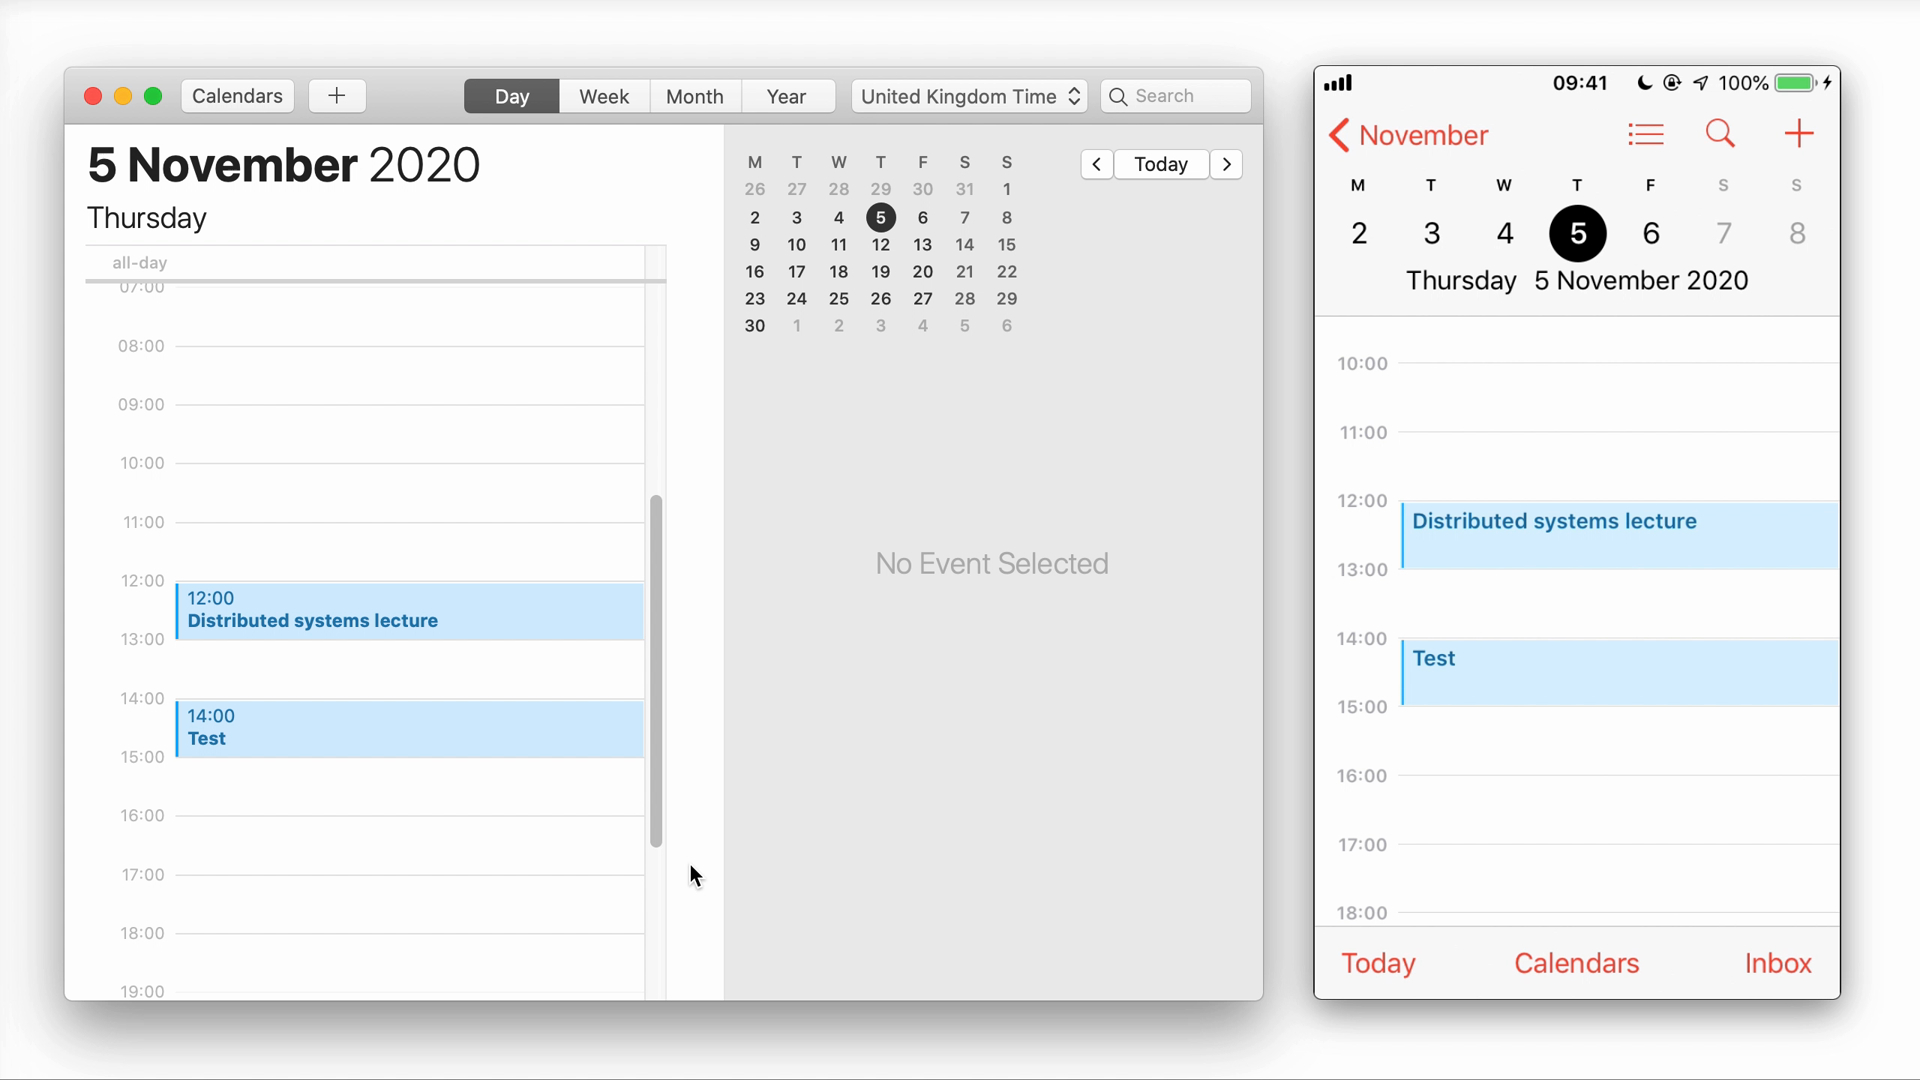
\includegraphics[width=\paperwidth]{images/calendar.png}};
    \end{tikzpicture}
\end{frame}
\inlineslide{s:calendar}{}\label{l:calendar}

Instead, calendar apps allow the user to read and write events in their calendar even while a device is offline, and they sync any updates between devices sometime later, in the background, when an internet connection is available.

This trade-off is known as the \emph{CAP theorem} (named after \emph{consistency}, \emph{availability}, and \emph{partition tolerance}), which states that if there is a network partition in a system, we must choose between one of the following options \citep{Gilbert:2002}:
\begin{enumerate}
    \item We can have linearizable consistency, but in this case, some replicas will not be able to respond to requests because they cannot communicate with a quorum.
        Not being able to respond to requests makes those nodes effectively unavailable.
    \item We can allow replicas to respond to requests even if they cannot communicate with other replicas.
        In this case, they continue to be available, but we cannot guarantee linearizability.
\end{enumerate}
Sometimes the CAP theorem is formulated as a choice of ``pick 2 out of 3'', but that framing is misleading.
A system can be both linearizable and available as long as there is no network partition, and the choice is forced only in the presence of a partition \citep{Kleppmann:2015}.

This trade-off is illustrated on \autoref{l:cap-theorem}, where node $C$ is unable to communicate with nodes $A$ and $B$.
On $A$ and $B$'s side of the partition, linearizable operations can continue as normal, because $A$ and $B$ constitute a quorum.
However, if $C$ wants to read the value of $x$, it must either wait (potentially indefinitely) until the network partition is repaired, or it must return its local value of $x$, which does not reflect the value previously written by $A$ on the other side of the partition.

\begin{frame}
    \label{s:cap-theorem}
    \frametitle{The CAP theorem}
    A system can be either strongly \textbf{Consistent} (linearizable) or \textbf{Available} in the presence of a network \textbf{Partition}
    \begin{center}
        \begin{tikzpicture}
            \node [rectangle,fill=red!10,draw] (node1) at (0,5.7) {node $A$};
            \node [rectangle,fill=red!10,draw] (node2) at (3,5.7) {node $B$};
            \node [rectangle,fill=red!10,draw] (node3) at (7,5.7) {node $C$};
            \draw (node1) -- (0,0.5);
            \draw (node2) -- (3,0.5);
            \draw (node3) -- (7,0.5);
            \draw [red,very thick,dashed] (5,0.5) -- (5,6);
            \node [rotate=270,red] at (4.7,3) {network partition};
            \node [op,text width=1.5cm] (op1) at (0,4.2) {$\mathsf{set}(x,v_1)$};
            \draw [bigarrow] (op1.north west) -- +(0.9,-0.3);
            \draw [revbigarrow] (op1.north east) -- +(0.9,0.3);
            \node [op,text width=1.9cm] (op2) at (0,1.8) {$\mathsf{get}(x) \rightarrow v_1$};
            \draw [bigarrow] (op2.north west) -- +(0.9,-0.3);
            \draw [revbigarrow] (op2.north east) -- +(0.9,0.3);
            \node [op,text width=1.9cm] (op3) at (3,1.8) {$\mathsf{get}(x) \rightarrow v_1$};
            \draw [bigarrow] (op3.south west) -- +(-0.9,-0.3);
            \draw [revbigarrow] (op3.south east) -- +(-0.9,0.3);
            \node [op,text width=1.9cm] (op4) at (7,1.8) {$\mathsf{get}(x) \rightarrow v_0$};
            \draw [messageloss] (op4.south west) -- +(-0.9,-0.3);
        \end{tikzpicture}
    \end{center}%
    $C$ must either wait indefinitely for the network to recover, or return a potentially stale value
\end{frame}
\inlineslide{s:cap-theorem}{}\label{l:cap-theorem}

The calendar app chooses option 2: it forgoes linearizability in favour of allowing the user to continue performing operations while a device is offline.
Many other systems similarly make this choice for various reasons.

The approach of allowing each replica to process both reads and writes based only on its local state, and without waiting for communication with other replicas, is called \emph{optimistic replication}.
A variety of consistency models have been proposed for optimistically replicated systems, with the best-known being \emph{eventual consistency}.

Eventual consistency is defined as: ``if no new updates are made to an object, eventually all reads will return the last updated value'' \citep{Vogels:2009}.
This is a very weak definition: what if the updates to an object never stop, so the premise of the statement is never true?
A slightly stronger consistency model called \emph{strong eventual consistency}, defined on \autoref{l:eventual-2}, is often more appropriate \citep{Shapiro:2011}.
It is based on the idea that as two replicas communicate, they \emph{converge} towards the same state.

\begin{frame}
    \label{s:eventual-2}
    \frametitle{Eventual consistency}
    Replicas process operations based only on their local state.\\[0.5em]
    If there are no more updates, \textbf{eventually} all replicas will be in the same state.
    (No guarantees how long it might take.)\\[0.5em]\pause
    \textbf{Strong eventual consistency}:
    \begin{itemize}
        \item \textbf{Eventual delivery:} every update made to one non-faulty replica is eventually processed by every non-faulty replica.\pause
        \item \textbf{Convergence:} any two replicas that have processed the same set of updates are in the same state\\
            (even if updates were processed in a different order).\\[0.5em]\pause
    \end{itemize}
    Properties:
    \begin{itemize}
        \item Does not require waiting for network communication
        \item Causal broadcast (or weaker) can disseminate updates\pause
        \item Concurrent updates $\Longrightarrow$ \textbf{conflicts} need to be resolved
    \end{itemize}
\end{frame}
\inlineslide{s:eventual-2}{}\label{l:eventual-2}

In both eventual consistency and strong eventual consistency, there is the possibility of different nodes concurrently updating the same object, leading to conflicts (as previously discussed on \autoref{l:concurrent-writes}).
Various algorithms have been developed to resolve those conflicts automatically \citep{Shapiro:2011}.

In the lecture I show a demo of a conflict in the eventually consistent calendar app: on one device, I update the time of an event, while concurrently on another device, I update the title of the same event.
After the two devices synchronise, the update of the time is applied to both devices, while the update of the title is discarded~-- or possibly the other way round.
The state of the two devices therefore converges~-- at the cost of a small amount of data loss.
This is the \emph{last writer wins} approach to conflict resolution that we have seen on \autoref{l:concurrent-writes} (assuming the update to the time is the ``last'' update in this example).
A more refined approach might merge the updates to the time and the title, as shown on \autoref{l:lecture-conflicts}.

\autoref{l:model-requirements} summarises some of the key properties of the consistency models we have seen, in descending order of the minimum strength of assumptions that they must make about the system model.

\begin{frame}
    \label{s:model-requirements}
    \frametitle{Summary of minimum system model requirements}
    \begin{tikzpicture}[remember picture,overlay]
        \node (highest) [xshift=5.3cm,yshift=1.5cm] at (current page.center) {};
        \node (lowest)  [xshift=5.3cm,yshift=-3cm] at (current page.center) {};
        \node [xshift=5.7cm,yshift=-0.75cm,rotate=90,blue,font=\footnotesize] at (current page.center) {strength of assumptions};
        \draw [-Stealth,very thick,blue] (lowest) -- (highest);
    \end{tikzpicture}%
    \rowcolors[]{2}{}{blue!10}%
    \renewcommand{\arraystretch}{1.5}%
    \begin{tabular}{>{\raggedright}p{3.7cm}|>{\raggedright}p{3cm}|>{\raggedright\arraybackslash}p{2.4cm}} % https://tex.stackexchange.com/a/2892
        \textbf{Problem} & \textbf{Must wait for communication} & \textbf{Requires synchrony} \\\hline
        atomic commit & all participating nodes & partially synchronous\pause\\
        consensus,\newline total order broadcast,\newline linearizable CAS & quorum & partially synchronous\pause\\
        linearizable get/set & quorum & asynchronous\pause\\
        eventual consistency,\newline causal broadcast,\newline FIFO broadcast & local replica only & asynchronous \\\hline
    \end{tabular}
\end{frame}
\inlineslide{s:model-requirements}{}\label{l:model-requirements}

% Note: the participants in atomic commit could be fault-tolerant services, not individual nodes

Atomic commit makes the strongest assumptions, since it must wait for communication with all nodes participating in a transaction (potentially all of the nodes in the system) in order to complete successfully.
Consensus, total order broadcast, and linearizable algorithms make weaker assumptions since they only require waiting for communication with a quorum, so they can tolerate some unavailable nodes.
The FLP result (\autoref{l:consensus-model}) showed us that consensus and total order broadcast require partial synchrony.
It can be shown that a linearizable CAS operation is equivalent to consensus \citep{Herlihy:1991}, and thus also requires partial synchrony.
On the other hand, the ABD algorithm for a linearizable register (supporting $\mathsf{get}$/$\mathsf{set}$ operations) is asynchronous, since it does not require any clocks or timeouts.
Finally, eventual consistency and strong eventual consistency make the weakest assumptions: operations can be processed without waiting for any communication with other nodes, and without any timing assumptions.
Similarly, in causal broadcast and weaker forms of broadcast (FIFO, reliable, etc.), a node broadcasting a message can immediately deliver it to itself without waiting for communication with other nodes, as discussed in \autoref{sec:delivery-order}; this corresponds to a replica immediately processing its own operations without waiting for communication with other replicas.

This hierarchy has some similarities to the concept of complexity classes of algorithms~-- for example, sorting generally is $O(n \log n)$~-- in the sense that it captures the unavoidable minimum communication and synchrony requirements for a range of common problems in distributed systems.

\subsection{Conflict resolution and CRDTs}\label{sec:collaboration}

There is a particular type of software that makes good use of eventual consistency, which my collaborators and I decided to call \emph{local-first software}~\citep{Kleppmann:2019}.
This is software running on end-user devices (laptop, smartphone, etc.) that first stores its data locally on the user's device, but also replicates that data to other devices when a network connection is available (perhaps via servers).
The aforementioned calendar app is an example of local-first software.

Local-first software contrasts with web applications such as Google Docs, which store all of their data on cloud servers.
Cloud storage makes it easy to share data with colleagues and access it from multiple devices, but it has the disadvantage that the software usually does not work offline.
Moreover, if a user gets locked out of their account or if the cloud service shuts down, they lose access to all of the data they have created.

Local-first software has several advantages over web apps: users can continue accessing their local copy of the data, even while they are offline or if they lose access to the cloud service.
This gives users greater control over their data while enabling similar collaboration features as in web apps.

\begin{frame}
    \label{s:local-first}
    \frametitle{Local-first software}
    \textbf{End-user device is a full replica}; servers are just for backup.\\
    ``Local-first'': a term introduced by me and my colleagues\\
    \url{https://www.inkandswitch.com/local-first/}\\[1em]
    Calendar app with cross-device sync is an example:\pause
    \begin{itemize}
        \item App works \textbf{offline} (can both read and modify data)
        \item \textbf{Fast}: no need to wait for network round-trip
        \item \textbf{Sync} with other devices when online
        \item \textbf{Real-time collaboration} with other users\pause
        \item \textbf{Longevity}: even if cloud service shuts down, you have a copy of your files on your own computer
        \item Supports \textbf{end-to-end encryption} for better security
        \item Simpler \textbf{programming model} than RPC
        \item \textbf{User control} and agency over their own data
    \end{itemize}
\end{frame}
\inlineslide{s:local-first}{}\label{l:local-first}

Collaboration software is a broad category of software that facilitates several people working together on some task.
This includes applications such as Google Docs/Office 365 (multi-user text documents, spreadsheets, presentations, etc.), Overleaf (collaborative {\LaTeX} documents), multi-user graphics software (e.g.\ Figma), project planning tools (e.g.\ Trello), note-taking apps (e.g.\ OneNote, Evernote, Notion), and shared calendars between colleagues or family members (like the calendar sync we saw on \autoref{l:calendar}).
Many of these are web apps, not local-first software, but similar approaches apply to both.

Modern collaboration software allows several people to update a document concurrently, without having to email files back and forth.
This makes collaboration another example of replication: each device on which a user has opened a document is a replica, and any updates made to one replica need to be sent over the network to the replicas on other devices.

In principle, it would be possible to use a linearizable replication scheme for collaboration software.
However, such software would be slow to use, since every read or write operation would have to contact a quorum of replicas; moreover, it would not work on a device that is offline.
Instead, for the sake of better performance and better robustness to network interruptions, most collaboration software uses optimistic replication that provides strong eventual consistency (\autoref{l:eventual-2}).

\begin{frame}
    \label{s:collaboration}
    \frametitle{Collaboration and conflict resolution}
    Nowadays we use a lot of \textbf{collaboration software}:
    \begin{itemize}
        \item \textbf{Examples:} calendar sync, text editors (Google Docs), spreadsheets, presentations, graphics apps\dots\pause
        \item Several users/devices working on a shared file/document
        \item Each user device has local replica of the data\pause
        \item Update local replica optimistically, sync with others asynchronously (waiting for round trip is too slow)\pause
        \item \textbf{Challenge:} how to reconcile concurrent updates?\\[1em]\pause
    \end{itemize}
    Families of \textbf{algorithms}:
    \begin{itemize}
        \item Conflict-free Replicated Data Types (\textbf{CRDTs})
            \begin{itemize}
                \item Operation-based
                \item State-based
            \end{itemize}
        \item Operational Transformation (\textbf{OT})
    \end{itemize}
\end{frame}
\inlineslide{s:collaboration}{}\label{l:collaboration}

In this lecture we will look at some algorithms that are used for this kind of collaboration.
As example, consider calendar sync again.
Two nodes initially start with the same calendar entry.
On node $A$, the title is changed from ``Lecture'' to ``Lecture 1'', and concurrently on node $B$ the time is changed from 12:00 to 10:00.
These two updates happen while the two nodes are temporarily unable to communicate, but eventually connectivity is restored and the two nodes sync their changes.
In the outcome shown on \autoref{l:lecture-conflicts}, the final calendar entry reflects both the change to the title and the change to the time.

\begin{frame}
    \label{s:lecture-conflicts}
    \frametitle{Conflicts due to concurrent updates}
    \begin{tikzpicture}
        \node [rectangle,fill=red!10,draw] (node1) at (0,6.4) {node $A$};
        \node [rectangle,fill=red!10,draw] (node2) at (6,6.4) {node $B$};
        \draw (node1) -- (0,-1.2);
        \draw (node2) -- (6,-1.2);
        \draw [red,very thick,dashed] (3,2.0) -- (3,6.6);
        \node [rotate=270,red] at (2.7,4.3) {network partition};
        \node [draw,fill=white] at (0,5) {\begin{minipage}{3.5cm}
            \inputminted[fontsize=\scriptsize]{json}{code/conflict1.json}
        \end{minipage}};
        \node<2-> [font=\footnotesize] at (-0.1,3.75) {\texttt{title = "Lecture 1"}};
        \node<2-> [draw,fill=white] at (0,2.5) {\begin{minipage}{3.5cm}
            \inputminted[fontsize=\scriptsize]{json}{code/conflict2.json}
        \end{minipage}};
        \node<4-> [draw,fill=white] at (0,0) {\begin{minipage}{3.5cm}
            \inputminted[fontsize=\scriptsize]{json}{code/conflict4.json}
        \end{minipage}};
        \node [draw,fill=white] at (6,5) {\begin{minipage}{3.5cm}
            \inputminted[fontsize=\scriptsize]{json}{code/conflict1.json}
        \end{minipage}};
        \node<3-> [font=\footnotesize] at (7.4,3.75) {\texttt{time = "10:00"}};
        \node<3-> [draw,fill=white] at (6,2.5) {\begin{minipage}{3.5cm}
            \inputminted[fontsize=\scriptsize]{json}{code/conflict3.json}
        \end{minipage}};
        \node<4-> [draw,fill=white] at (6,0) {\begin{minipage}{3.5cm}
            \inputminted[fontsize=\scriptsize]{json}{code/conflict4.json}
        \end{minipage}};
        \draw<4-> [doublebigarrow] (0,1.25) -- node [above] {sync} (6,1.25);
    \end{tikzpicture}
\end{frame}
\inlineslide{s:lecture-conflicts}{}\label{l:lecture-conflicts}

This scenario is an example of \emph{conflict resolution}, which occurs whenever several concurrent writes to the same object need to be integrated into a single final state (see also \autoref{l:concurrent-writes}).
\emph{Conflict-free replicated data types}, or \emph{CRDTs} for short, are a family of algorithms that perform such conflict resolution \citep{Shapiro:2011}.
A CRDT is a replicated object that an application accesses though the object-oriented interface of an abstract datatype, such as a set, list, map, tree, graph, counter, etc.

\autoref{l:op-crdt-map} shows an example of a CRDT that provides a map from keys to values.
The application can invoke two types of operation: reading the value for a given key, and setting the value for a given key (which adds the key if it is not already present).
In other words, each key has an associated register, as discussed in \autoref{sec:remote-state}.

The local state at each node consists of the set $\mathit{values}$ containing $(\mathit{timestamp}, \mathit{key}, \mathit{value})$ triples.
Reading the value for a given key is a purely local operation that only inspects $\mathit{values}$ on the current node, and performs no network communication.
The algorithm preserves the invariant that $\mathit{values}$ contains at most one element for any given key.
Therefore, when reading the value for a key, the value is unique if it exists.

\begin{frame}
    \label{s:op-crdt-map}
    \frametitle{Operation-based map CRDT}
    \footnotesize
    \begin{algorithmic}
        \On{initialisation}
            \State $\mathit{values} := \{\}$
        \EndOn
        \State
        \On{request to read value for key $k$}
            \State \textbf{if} $\exists t,v.\; (t,k,v) \in \mathit{values}$ \textbf{then return} $v$ \textbf{else return} $\mathsf{null}$
        \EndOn
        \State
        \On{request to set key $k$ to value $v$}
            \State $t := \mathrm{newTimestamp}()$ \Comment{globally unique, e.g. Lamport timestamp}
            \State \textbf{broadcast} $(\mathsf{set}, t, k, v)$ by reliable broadcast (including to self)
        \EndOn
        \State
        \On{delivering $(\mathsf{set},t,k,v)$ by reliable broadcast}
            \State $\mathit{previous} := \{(t',k',v') \in \mathit{values} \mid k' = k\}$
            \If{$\mathit{previous} = \{\} \;\vee\; \forall (t',k',v') \in \mathit{previous}.\; t' < t$}
                \State $\mathit{values} := (\mathit{values} \setminus \mathit{previous}) \,\cup\, \{(t,k,v)\}$
            \EndIf
        \EndOn
    \end{algorithmic}
\end{frame}
\inlineslide{s:op-crdt-map}{}\label{l:op-crdt-map}

To update the value for a given key, we create a globally unique timestamp for the operation~-- a Lamport timestamp (\autoref{l:lamport-definition}) is a good choice~-- and then broadcast a message containing the timestamp, key, and value.
When that message is delivered, we check if the local copy of $\mathit{values}$ already contains an entry with a higher timestamp for the same key; if so, we ignore the message, because the value with the higher timestamp takes precedence.
Otherwise we remove the previous value (if any), and add the new $(\mathit{timestamp}, \mathit{key}, \mathit{value})$ triple to $\mathit{values}$.
This means that we resolve concurrent updates to the same key using the last-writer-wins (LWW) approach that we saw on \autoref{l:concurrent-writes}.

\begin{frame}
    \label{s:op-crdt}
    \frametitle{Operation-based CRDTs}
    Reliable broadcast may deliver updates in any order:
    \begin{itemize}
        \item broadcast $(\mathsf{set}, t_1, \text{``title''}, \text{``Lecture 1''})$
        \item broadcast $(\mathsf{set}, t_2, \text{``time''}, \text{``10:00''})$\\[1em]\pause
    \end{itemize}
    Recall \textbf{strong eventual consistency}:
    \begin{itemize}
        \item \textbf{Eventual delivery:} every update made to one non-faulty replica is eventually processed by every non-faulty replica.
        \item \textbf{Convergence:} any two replicas that have processed the same set of updates are in the same state\\[1em]\pause
    \end{itemize}
    CRDT algorithm implements this:
    \begin{itemize}
        \item Reliable broadcast ensures every operation is eventually delivered to every (non-crashed) replica\pause
        \item Applying an operation is \textbf{commutative}: order of delivery doesn't matter
    \end{itemize}
\end{frame}
\inlineslide{s:op-crdt}{}\label{l:op-crdt}

This algorithm is an example of an approach that we hinted at on \autoref{l:causal-replication}, namely, a method for performing replication using reliable broadcast, without requiring totally ordered delivery.
It is an \emph{operation-based} CRDT because each broadcast message contains a description of an update operation (as opposed to \emph{state-based} CRDTs that we will see shortly).
It allows operations to complete without network connectivity, because the sender of a reliable broadcast can immediately deliver a message to itself, and send it to other nodes sometime later.
Moreover, even though messages may be delivered in different orders on different replicas, the algorithm ensures strong eventual consistency because the function that updates a replica's state is commutative.

\supervision{
    Prove that the operation-based map CRDT algorithm provides strong eventual consistency.
}{
    The \emph{eventual delivery} property of strong eventual consistency holds because when a message is delivered by one non-faulty node, reliable broadcast ensures that it will also be delivered by all other non-faulty nodes.
    Therefore, each update applied on one non-faulty replica is also applied by every other non-faulty replica.

    To prove the \emph{convergence} property, we must show that any two replicas that have processed the same set of updates are in the same state.
    Note that the replica state $\mathit{values}$ is determined entirely and deterministically by the sequence of messages delivered by reliable broadcast.
    Consider two replicas, $A$ and $B$, on which the broadcast protocol has delivered the same set of messages; that is, their sequences of deliveries contain the same messages, and $A$'s sequence of deliveries is a permutation of $B$'s sequence of deliveries.
    Then we must show that processing the messages in $A$'s delivery order results in the same state as processing the messages in $B$'s delivery order.

    We can transform $A$'s sequence of deliveries into $B$'s sequence of deliveries by repeatedly performing pairwise swaps of two adjacent messages in the sequence, since one is a permutation of the other.
    Let $a$ and $b$ be any two such messages being swapped.
    To show convergence, we must prove commutativity: that is, processing first $a$ and then $b$ (in any replica state) has the same effect on the state as processing first $b$ then $a$.
    If this property holds, then each of the pairwise swaps that we make has no effect on the final state.

    To prove commutativity, let $a = (\mathsf{set}, t_a, k_a, v_a)$ and $b = (\mathsf{set}, t_b, k_b, v_b)$.
    We have $t_a \ne t_b$ due to the assumption of globally unique timestamps and because reliable broadcast does not duplicate messages.
    Assume $t_a < t_b$ without loss of generality.
    Let $\mathit{values}$ be the state of both replicas immediately before $a$ or $b$ are processed.

    Consider first the case where $k_a \ne k_b$.
    The pseudocode for delivering a $\mathsf{set}$ message only reads or modifies tuples in $\mathit{values}$ that contain the key in the message.
    Thus, two messages containing different keys can be processed in either order without affecting the outcome.

    In the case where $k_a=k_b$ we consider the following cases:
    \begin{enumerate}
        \item $\nexists t,v.\; (t,k_a,v) \in \mathit{values}.$

            Consider a replica that first processes $a$, then $b$.
            After processing $a$, the replica state is $\mathit{values} \cup \{(t_a,k_a,v_a)\}$.
            After processing $b$, the replica state is $\mathit{values} \cup \{(t_b,k_b,v_b)\}$.

            Next, consider a replica that first processes $b$, then $a$.
            After processing $b$, the replica state is $\mathit{values} \cup \{(t_b,k_b,v_b)\}$.
            After processing $a$, the replica state remains $\mathit{values} \cup \{(t_b,k_b,v_b)\}$ since $t_a < t_b$.
            Thus, both delivery orders lead to the same state.

        \item There exist $t,v$ such that $(t,k_a,v) \in \mathit{values}$.
            By uniqueness of timestamps, $t \ne t_a$ and $t \ne t_b$.
            We then consider further cases:

            \begin{enumerate}
                \item $t < t_a < t_b$.

                    A replica that first processes $a$ will first be in state $\mathit{values} \setminus \{(t,k_a,v)\} \cup \{(t_a,k_a,v_a)\}$, and then in state $\mathit{values} \setminus \{(t,k_a,v)\} \cup \{(t_b,k_b,v_b)\}$ after processing $b$.

                    A replica that first processes $b$ will first be in state $\mathit{values} \setminus \{(t,k_a,v)\} \cup \{(t_b,k_b,v_b)\}$, and then remain in that state after processing $a$.
                \item $t_a < t < t_b$.

                    A replica that first processes $a$ will remain in state $\mathit{values}$ after processing $a$.
                    After processing $b$ it moves to state $\mathit{values} \setminus \{(t,k_a,v)\} \cup \{(t_b,k_b,v_b)\}$.

                    A replica that first processes $b$ will first be in state $\mathit{values} \setminus \{(t,k_a,v)\} \cup \{(t_b,k_b,v_b)\}$, and then remain in that state after processing $a$.
                \item $t_a < t_b < t$.
                    Then processing $a$ and $b$ leaves the replica state unchanged, regardless of the order in which they are processed.
            \end{enumerate}
    \end{enumerate}
    In all of these cases, the state of a replica after processing $a$ then $b$ is the same as the state of a replica after processing $b$ then $a$.
    Therefore, $a$ and $b$ commute in all replica states, and therefore the algorithm ensures convergence.
}

\supervision{
    Give pseudocode for a variant of the operation-based map CRDT algorithm that has multi-value register semantics instead of last-writer-wins semantics; that is, when there are several concurrent updates for the same key, the algorithm should preserve all of those updates rather than preserving only the one with the greatest timestamp.
}{
    Note that this algorithm uses causal broadcast to ensure that when one updates overwrites another, the causally later (overwriting) update is delivered after the update that it overwrites. We extend the broadcast message to include a set $T$, which is the set of timestamps of causally prior operations that are overwritten by a particular $\mathsf{set}$ operation. This way, when a broadcast message is delivered, we know which values were written by operations that happened before this $\mathsf{set}$ operation, and which operations were concurrent.

    \begin{algorithmic}
        \On{initialisation}
            \State $\mathit{values} := \{\}$
        \EndOn
        \State
        \On{request to read value for key $k$}
            \State \textbf{return} $\{v \mid \exists t.\; (t,k,v) \in \mathit{values}\}$
        \EndOn
        \State
        \On{request to set key $k$ to value $v$}
            \State $T := \{t \mid \exists v'.\; (t,k,v') \in \mathit{values}\}$
            \State $t := \mathrm{newTimestamp}()$ \Comment{globally unique, e.g. Lamport timestamp~~~~~~~~~~~~~~~~~~~~~~~~~~~~~~~~~~~~~}
            \State \textbf{broadcast} $(\mathsf{set},T,t,k,v)$ by causal broadcast (including to self)
        \EndOn
        \State
        \On{delivering $(\mathsf{set},T,t,k,v)$ by causal broadcast}
            \State $\mathit{values} := \{(t',k',v') \in \mathit{values} \mid t' \notin T\} \,\cup\, \{(t,k,v)\}$
        \EndOn
    \end{algorithmic}
}

\begin{frame}
    \label{s:state-crdt-map}
    \frametitle{State-based map CRDT}
    \footnotesize
    The operator $\sqcup$ merges two states $s_1$ and $s_2$ as follows:
    \[ s_1 \sqcup s_2 = \{(t,k,v) \in (s_1 \cup s_2) \mid \nexists (t',k',v') \in (s_1 \cup s_2).\; k' = k \wedge t' > t\} \]
    \begin{algorithmic}
        \On{initialisation}
            \State $\mathit{values} := \{\}$
        \EndOn
        \State
        \On{request to read value for key $k$}
            \State \textbf{if} $\exists t,v.\; (t,k,v) \in \mathit{values}$ \textbf{then return} $v$ \textbf{else return} $\mathsf{null}$
        \EndOn
        \State
        \On{request to set key $k$ to value $v$}
            \State $t := \mathrm{newTimestamp}()$ \Comment{globally unique, e.g. Lamport timestamp}
            \State $\mathit{values} := \{(t',k',v') \in \mathit{values} \mid k' \neq k\} \,\cup\, \{(t,k,v)\}$
            \State \textbf{broadcast} $\mathit{values}$ by best-effort broadcast
        \EndOn
        \State
        \On{delivering $V$ by best-effort broadcast}
            \State $\mathit{values} := \mathit{values} \sqcup V$
        \EndOn
    \end{algorithmic}
\end{frame}
\inlineslide{s:state-crdt-map}{}\label{l:state-crdt-map}

An alternative CRDT algorithm for the same map datatype is shown on \autoref{l:state-crdt-map}.
The definition of $\mathit{values}$ and the function for reading the value for a key is the same as on \autoref{l:op-crdt-map}.
However, updates are handled differently: instead of broadcasting each operation, we directly update $\mathit{values}$ and then broadcast the whole of $\mathit{values}$.
On delivering this message at another replica, we merge together the two replicas' states using a merge function $\sqcup$.
This merge function compares the timestamps of entries with the same key, and keeps those with the greater timestamp.
This approach of broadcasting the entire replica state and merging it with another replica's state is called a \emph{state-based CRDT}.

\begin{frame}
    \label{s:state-crdt}
    \frametitle{State-based CRDTs}
    Merge operator $\sqcup$ must satisfy: $\forall s_1, s_2, s_3$\dots
    \begin{itemize}
        \item \textbf{Commutative}: $s_1 \sqcup s_2 = s_2 \sqcup s_1.$
        \item \textbf{Associative}: $(s_1 \sqcup s_2) \sqcup s_3 = s_1 \sqcup (s_2 \sqcup s_3).$
        \item \textbf{Idempotent}: $s_1 \sqcup s_1 = s_1.$\\[1em]\pause
    \end{itemize}
    State-based versus operation-based:
    \begin{itemize}
        \item Op-based CRDT typically has smaller messages
        \item State-based CRDT can tolerate message loss/duplication\\[1em]\pause
    \end{itemize}
    Not necessarily uses broadcast:
    \begin{itemize}
        \item Can also merge concurrent updates to replicas e.g. in quorum replication, anti-entropy, \dots
    \end{itemize}
\end{frame}
\inlineslide{s:state-crdt}{}\label{l:state-crdt}

The downside of the state-based approach is that the broadcast messages are likely to be larger than in the operation-based approach.
The advantage of the state-based approach is that it can tolerate lost or duplicated messages: as long as two replicas eventually succeed in exchanging their latest states, they will converge to the same state, even if some earlier messages were lost.
Duplicated messages are also fine because the merge operator is idempotent (cf.\ \autoref{l:idempotence}).
This is why a state-based CRDT can use unreliable best-effort broadcast, while an operation-based CRDT requires reliable broadcast (and some even require causal broadcast).

Moreover, state-based CRDTs are not limited to replication systems that use broadcast.
Other methods of replication, such as the quorum write algorithms and anti-entropy protocols we saw in \autoref{sec:replication}, can also use CRDTs for conflict resolution (see \autoref{l:reconcile}).

\subsection{Collaborative text editing}

As another example of concurrent updates and the need for conflict resolution, we will consider collaborative text editors such as Google Docs.
When you type in a Google Doc, the keystrokes are immediately applied to the local copy of the document in your web browser, without waiting for them to sync to a server or any other users.
This means that when two users are typing concurrently, their documents can temporarily diverge; as network communication takes place, the system needs to ensure that all users converge to the same view of the document.

\begin{frame}[plain]
    \label{s:google-docs}
    \begin{tikzpicture}[remember picture,overlay]
        \node at (current page.center) {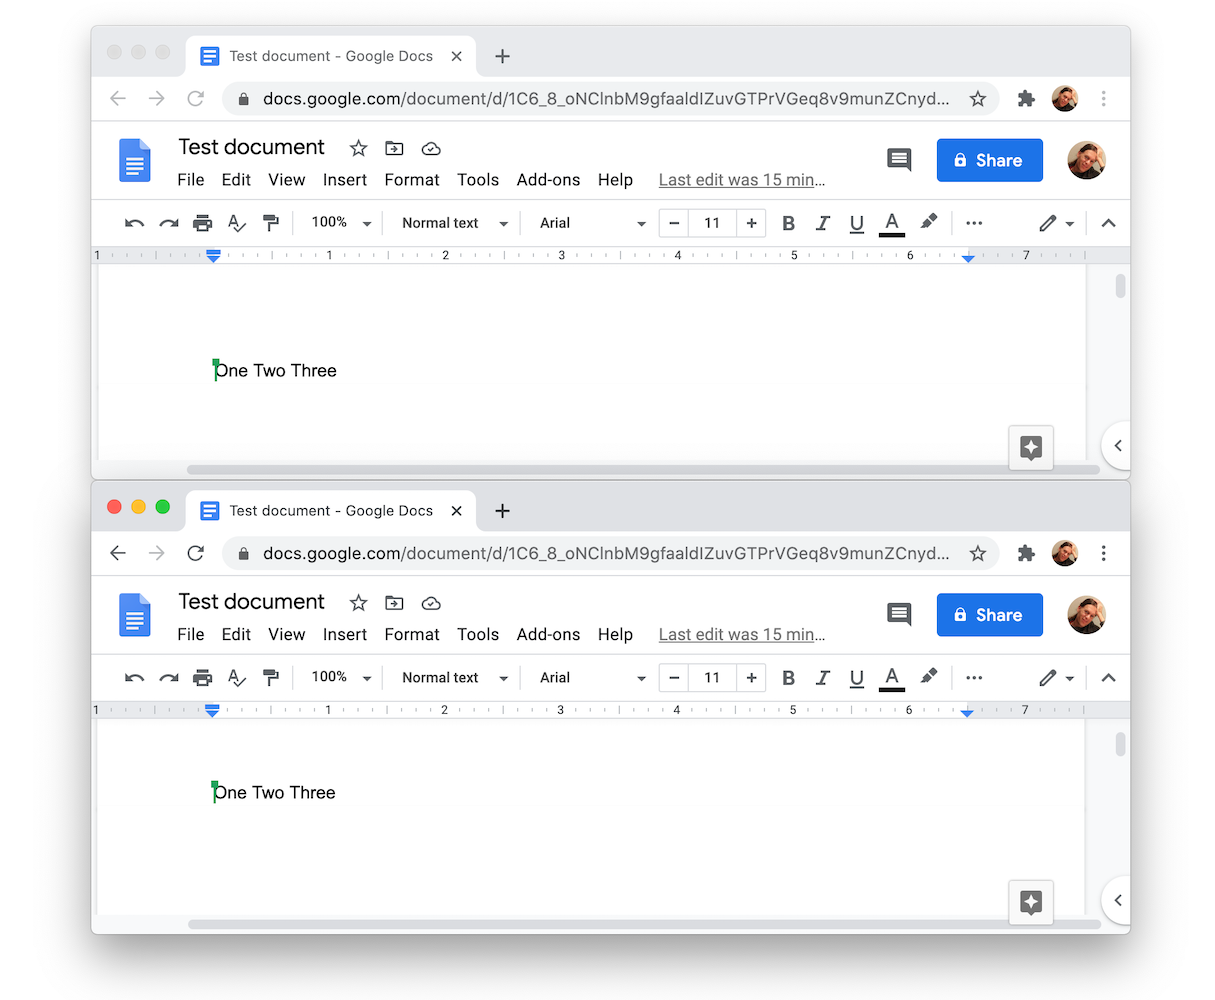
\includegraphics[height=\paperheight]{images/google-docs.png}};
    \end{tikzpicture}
\end{frame}
\inlineslide{s:google-docs}{}\label{l:google-docs}

% Use Apple's Network Link Conditioner (part of the Additional Tools for Xcode package) to disconnect the network while demoing Google Docs
% https://apple.stackexchange.com/questions/24066/how-to-simulate-slow-internet-connections-on-the-mac

We can think of a collaboratively editable text document as a list of characters, where each user can insert or delete characters at any index in the list.
Fonts, formatting, embedded images, tables, and so on add further complexity, so we will just concentrate on plain text for now.
When several users may concurrently update a text document, a particular problem arises, which is demonstrated in the example on \autoref{l:text-editing}.

\begin{frame}
    \label{s:text-editing}
    \frametitle{Collaborative text editing: the problem}
    \begin{center}
        % ampersand replacement: https://tex.stackexchange.com/questions/208408/tikz-matrix-undefined-control-sequence
        \begin{tikzpicture}[ampersand replacement=\&]
            \tikzstyle{state}=[draw,fill=white,matrix,column sep={20pt,between origins}]
            \tikzstyle{val}=[draw,anchor=base,minimum width=20pt,text height=8pt,text depth=3pt]
            \tikzstyle{oid}=[anchor=base,font=\footnotesize]
            \node [rectangle,fill=red!10,draw] (node1) at (0,6.4) {user $A$};
            \node [rectangle,fill=red!10,draw] (node2) at (6,6.4) {user $B$};
            \draw (node1) -- (0,-1);
            \draw (node2) -- (6,-1);
            \draw [red,very thick,dashed] (3,2.0) -- (3,6.6);
            \node [rotate=270,red] at (2.7,4.3) {network partition};
            \node (a1) at (0,5) [state] {
                \node [val] {\texttt{B}}; \&
                \node [val] {\texttt{C}}; \\
                \node [oid] {0}; \&
                \node [oid] {1}; \\
            };
            \path<2-> (0,3.9) node [right,font=\footnotesize] {$\mathsf{insert}(0, \text{``A''})$};
            \node<2-> (a2) at (0,2.8) [state] {
                \node [val] {\texttt{A}}; \&
                \node [val] {\texttt{B}}; \&
                \node [val] {\texttt{C}}; \\
                \node [oid] {0}; \&
                \node [oid] {1}; \&
                \node [oid] {2}; \\
            };
            \node<5-> (a3) at (0,0) [state] {
                \node [val] {\texttt{A}}; \&
                \node [val] {\texttt{B}}; \&
                \node [val,fill=red!10] {\texttt{D}}; \&
                \node [val,fill=red!10] {\texttt{C}}; \\
                \node [oid] {0}; \&
                \node [oid] {1}; \&
                \node [oid,fill=red!10] {2}; \&
                \node [oid,fill=red!10] {3}; \\
            };
            \node (b1) at (6,5) [state] {
                \node [val] {\texttt{B}}; \&
                \node [val] {\texttt{C}}; \\
                \node [oid] {0}; \&
                \node [oid] {1}; \\
            };
            \path<3-> (6,3.9) node [right,font=\footnotesize] {$\mathsf{insert}(2, \text{``D''})$};
            \node<3-> (b2) at (6,2.8) [state] {
                \node [val] {\texttt{B}}; \&
                \node [val] {\texttt{C}}; \&
                \node [val] {\texttt{D}}; \\
                \node [oid] {0}; \&
                \node [oid] {1}; \&
                \node [oid] {2}; \\
            };
            \node<4-> (b3) at (6,0) [state] {
                \node [val] {\texttt{A}}; \&
                \node [val] {\texttt{B}}; \&
                \node [val] {\texttt{C}}; \&
                \node [val] {\texttt{D}}; \\
                \node [oid] {0}; \&
                \node [oid] {1}; \&
                \node [oid] {2}; \&
                \node [oid] {3}; \\
            };
            \draw<4-> (0,1.3) edge [bigarrow,out=0,in=160]
                node [above,near start,font=\footnotesize] {$(\mathsf{insert}, 0, \text{``A''})$} (b3.north west);
            \draw<5-> (6,1.3) edge [bigarrow,out=180,in=20]
                node [above,near start,font=\footnotesize] {$(\mathsf{insert}, 2, \text{``D''})$} (a3.north east);
            \useasboundingbox (-2,-1) -- (9,-1);
        \end{tikzpicture}
    \end{center}
\end{frame}
\inlineslide{s:text-editing}{}\label{l:text-editing}

In this example, two users $A$ and $B$ both start with the same document, ``BC''.
User $A$ adds the character ``A'' at the beginning of the document, so that it reads ``ABC''.
Concurrently, user $B$ adds the character ``D'' at the end of the document, so that it reads ``BCD''.
As $A$ and $B$ merge their edits, we would expect that the final document should read ``ABCD''.

On \autoref{l:text-editing}, the users' replicas communicate by sending each other the operations they have performed.
User $A$ sends $(\mathsf{insert}, 0, \text{``A''})$ to $B$, and $B$ applies this operation, leading to the desired outcome ``ABCD''.
However, when $B$ sends $(\mathsf{insert}, 2, \text{``D''})$ to $A$, and $A$ inserts the character ``D'' at index 2, the result is ``ABDC'', not the expected ``ABCD''.

The problem is that at the time when $B$ performed the operation $\mathsf{insert}(2, \text{``D''})$, index 2 referred to the position after character ``C''.
However, $A$'s concurrent insertion at index 0 had the effect of increasing the indexes of all subsequent characters by 1, so the position after ``C'' is now index 3, not index 2.

\emph{Operational transformation} is one approach that is used to solve this problem.
There is a family of different algorithms that use this approach and that vary in the details of how they resolve conflicts.
But the general principle they have in common is illustrated on \autoref{l:op-transform}.

\begin{frame}
    \label{s:op-transform}
    \frametitle{Operational transformation}
    \begin{center}
        % ampersand replacement: https://tex.stackexchange.com/questions/208408/tikz-matrix-undefined-control-sequence
        \begin{tikzpicture}[ampersand replacement=\&]
            \tikzstyle{state}=[draw,fill=white,matrix,column sep={20pt,between origins}]
            \tikzstyle{val}=[draw,anchor=base,minimum width=20pt,text height=8pt,text depth=3pt]
            \tikzstyle{oid}=[anchor=base,font=\footnotesize]
            \node [rectangle,fill=red!10,draw] (node1) at (0,6.7) {user $A$};
            \node [rectangle,fill=red!10,draw] (node2) at (6,6.7) {user $B$};
            \draw (node1) -- (0,-1);
            \draw (node2) -- (6,-1);
            \path (0,5.9) node [right,font=\footnotesize] {$\mathsf{insert}(0, \text{``A''})$};
            \node (a1) at (0,4.8) [state] {
                \node [val] {\texttt{A}}; \&
                \node [val] {\texttt{B}}; \&
                \node [val] {\texttt{C}}; \\
                \node [oid] {0}; \&
                \node [oid] {1}; \&
                \node [oid] {2}; \\
            };
            \node<2-> (a2) at (0,1.8) [draw,fill=white,text width=3cm,align=left,font=\footnotesize] {
                $T((\mathsf{insert}, 2, \text{``D''}),$ \\
                $\quad(\mathsf{insert}, 0, \text{``A''})) =$ \\
                $\quad(\mathsf{insert}, 3, \text{``D''})$
            };
            \node<3-> (b2) at (6,1.8) [draw,fill=white,text width=3cm,align=left,font=\footnotesize] {
                $T((\mathsf{insert}, 0, \text{``A''}),$ \\
                $\quad(\mathsf{insert}, 2, \text{``D''})) =$ \\
                $\quad(\mathsf{insert}, 0, \text{``A''})$
            };
            \node<2-> (a3) at (0,0) [state] {
                \node [val] {\texttt{A}}; \&
                \node [val] {\texttt{B}}; \&
                \node [val] {\texttt{C}}; \&
                \node [val] {\texttt{D}}; \\
                \node [oid] {0}; \&
                \node [oid] {1}; \&
                \node [oid] {2}; \&
                \node [oid] {3}; \\
            };
            \path (6,5.9) node [right,font=\footnotesize] {$\mathsf{insert}(2, \text{``D''})$};
            \node (b1) at (6,4.8) [state] {
                \node [val] {\texttt{B}}; \&
                \node [val] {\texttt{C}}; \&
                \node [val] {\texttt{D}}; \\
                \node [oid] {0}; \&
                \node [oid] {1}; \&
                \node [oid] {2}; \\
            };
            \node<3-> (b3) at (6,0) [state] {
                \node [val] {\texttt{A}}; \&
                \node [val] {\texttt{B}}; \&
                \node [val] {\texttt{C}}; \&
                \node [val] {\texttt{D}}; \\
                \node [oid] {0}; \&
                \node [oid] {1}; \&
                \node [oid] {2}; \&
                \node [oid] {3}; \\
            };
            \draw<3-> (0,3.3) edge [bigarrow,out=0,in=160]
                node [above,near start,font=\footnotesize] {$(\mathsf{insert}, 0, \text{``A''})$} (b2.north west);
            \draw<2-> (6,3.3) edge [bigarrow,out=180,in=20]
                node [above,near start,font=\footnotesize] {$(\mathsf{insert}, 2, \text{``D''})$} (a2.north east);
            \useasboundingbox (-2,0) -- (8,0);
        \end{tikzpicture}
    \end{center}
\end{frame}
\inlineslide{s:op-transform}{}\label{l:op-transform}

A node keeps track of the history of operations it has performed.
When a node receives another node's operation that is concurrent to one or more of its own operations, it \emph{transforms} the incoming operation relative to its own, concurrent operations.

The function $T(\mathit{op}_1, \mathit{op}_2)$ takes two operations: $\mathit{op}_1$ is an incoming operation, and $\mathit{op}_2$ is a concurrent local operation.
$T$ returns a transformed operation $\mathit{op}_1'$ such that applying $\mathit{op}_1'$ to the local state has the effect originally intended by $\mathit{op}_1$.
For example, if $\mathit{op}_1 = (\mathsf{insert}, 2, \text{``D''})$ and $\mathit{op}_2 = (\mathsf{insert}, 0, \text{``A''})$ then the transformed operation is $T(\mathit{op}_1, \mathit{op}_2) = (\mathsf{insert}, 3, \text{``D''})$ because the original insertion $\mathit{op}_1$ at index 2 now needs to be instead be performed at index 3 due to the concurrent insertion at index 0.
On the other hand, $T(\mathit{op}_2, \mathit{op}_1) = \mathit{op}_2$ returns the unmodified $\mathit{op}_2$ because the insertion at index 0 is not affected by a concurrent insertion later in the document.

% TODO: give pseudocode for T

The transformation function becomes more complicated when deletions, formatting etc.\ are taken into account, and we will skip the details.
However, this approach is used in practice: for example, the conflict resolution algorithm in Google Docs uses an operational transformation approach based on the Xerox PARC research system Jupiter \citep{Nichols:1995}.
A limitation of this approach is that it requires communication between users to use total order broadcast, requiring the use of a designated leader node to sequence the updates, or a consensus algorithm as in \autoref{sec:consensus}.

An alternative to operational transformation, which avoids the need for total order broadcast, is to use a CRDT for text editing.
Rather than identifying positions in the text using indexes, and thus necessitating operational transformation, text editing CRDTs work by attaching a unique identifier to each character.
These identifiers remain unchanged, even as surrounding characters are inserted or deleted.

Several constructions for these unique identifiers have been proposed, one of which is illustrated on \autoref{l:text-crdt}.
Here, each character is assigned a rational number $i \in \mathbb{Q}$ with $0 < i < 1$, where 0 represents the beginning of the document, 1 is the end, and numbers in between identify the characters in the document in ascending order.
We also use the symbol $\vdash$ to represent the beginning of document and $\dashv$ to represent the end; these symbols are part of the algorithm's internal state, not visible to the user.

When we want to insert a new character between two existing adjacent characters with position numbers $i$ and $j$, we can assign that new character a position number of $\frac{i+j}{2}$, which always lies between $i$ and $j$.
This new position always exists, provided that we use arbitrary-precision arithmetic (floating-point numbers have limited precision, so they would no longer work once the intervals get too small).
It is possible for two different nodes to generate characters with the same position number if they concurrently insert at the same position, so we can use the ID of the node that generated a character to break ties for any characters that have the same position number.
Using this approach, conflict resolution becomes easy: an insertion with a particular position number can simply be broadcast to other replicas, which then add that character to their set of characters, and sort by position number to obtain the current document.

\begin{frame}
    \label{s:text-crdt}
    \frametitle{Text editing CRDT}
    \begin{center}
        \begin{tikzpicture}[ampersand replacement=\&]
            \tikzstyle{state}=[draw,fill=white,matrix,column sep={20pt,between origins}]
            \tikzstyle{val}=[draw,anchor=base,minimum width=20pt,text height=8pt,text depth=3pt]
            \tikzstyle{oid}=[anchor=base,font=\scriptsize]
            \node [rectangle,fill=red!10,draw] (node1) at (0,6.4) {user $A$};
            \node [rectangle,fill=red!10,draw] (node2) at (6.5,6.4) {user $B$};
            \draw (node1) -- (0,-1);
            \draw (node2) -- (6.5,-1);
            \node (a1) at (0,5) [state] {
                \node [val] {$\vdash$}; \&
                \node [val] {\texttt{B}}; \&
                \node [val] {\texttt{C}}; \&
                \node [val] {$\dashv$}; \\
                \node [oid] {0.0}; \&
                \node [oid] {0.5}; \&
                \node [oid] {0.75}; \&
                \node [oid] {1.0}; \\
            };
            \path<2-> (0,3.9) node [right,font=\footnotesize] {$\mathsf{insert}(0.25, \text{``A''})$};
            \node<2-> (a2) at (0,2.8) [state] {
                \node [val] {$\vdash$}; \&
                \node [val] {\texttt{A}}; \&
                \node [val] {\texttt{B}}; \&
                \node [val] {\texttt{C}}; \&
                \node [val] {$\dashv$}; \\
                \node [oid] {0.0}; \&
                \node [oid] {0.25}; \&
                \node [oid] {0.5}; \&
                \node [oid] {0.75}; \&
                \node [oid] {1.0}; \\
            };
            \node<4-> (a3) at (0,0) [state] {
                \node [val] {$\vdash$}; \&
                \node [val] {\texttt{A}}; \&
                \node [val] {\texttt{B}}; \&
                \node [val] {\texttt{C}}; \&
                \node [val] {\texttt{D}}; \&
                \node [val] {$\dashv$}; \\
                \node [oid] {0.0}; \&
                \node [oid] {0.25}; \&
                \node [oid] {0.5}; \&
                \node [oid] {0.75}; \&
                \node [oid] {0.875}; \&
                \node [oid] {1.0}; \\
            };
            \node (b1) at (6.5,5) [state] {
                \node [val] {$\vdash$}; \&
                \node [val] {\texttt{B}}; \&
                \node [val] {\texttt{C}}; \&
                \node [val] {$\dashv$}; \\
                \node [oid] {0.0}; \&
                \node [oid] {0.5}; \&
                \node [oid] {0.75}; \&
                \node [oid] {1.0}; \\
            };
            \path<3-> (6.5,3.9) node [left,font=\footnotesize] {$\mathsf{insert}(0.875, \text{``D''})$};
            \node<3-> (b2) at (6.5,2.8) [state] {
                \node [val] {$\vdash$}; \&
                \node [val] {\texttt{B}}; \&
                \node [val] {\texttt{C}}; \&
                \node [val] {\texttt{D}}; \&
                \node [val] {$\dashv$}; \\
                \node [oid] {0.0}; \&
                \node [oid] {0.5}; \&
                \node [oid] {0.75}; \&
                \node [oid] {0.875}; \&
                \node [oid] {1.0}; \\
            };
            \node<5-> (b3) at (6.5,0) [state] {
                \node [val] {$\vdash$}; \&
                \node [val] {\texttt{A}}; \&
                \node [val] {\texttt{B}}; \&
                \node [val] {\texttt{C}}; \&
                \node [val] {\texttt{D}}; \&
                \node [val] {$\dashv$}; \\
                \node [oid] {0.0}; \&
                \node [oid] {0.25}; \&
                \node [oid] {0.5}; \&
                \node [oid] {0.75}; \&
                \node [oid] {0.875}; \&
                \node [oid] {1.0}; \\
            };
            \draw<5-> (0,1.3) edge [bigarrow,out=0,in=160]
                node [above right,at start,font=\footnotesize] {$(\mathsf{insert}, 0.25, \text{``A''})$} (b3.north west);
            \draw<4-> (6.5,1.3) edge [bigarrow,out=180,in=20]
                node [above left,at start,font=\footnotesize] {$(\mathsf{insert}, 0.875, \text{``D''})$} (a3.north east);
            \useasboundingbox (-2.3,0) -- (8.8,0);
        \end{tikzpicture}
    \end{center}
\end{frame}
\inlineslide{s:text-crdt}{}\label{l:text-crdt}

This algorithm is shown on Slides \ref{l:text-crdt-alg1} and \ref{l:text-crdt-alg2}.
The state of a replica is the set $\mathit{chars}$, which contains $(\mathit{position}, \mathit{nodeId}, \mathit{character})$ triples.
The function \textsc{ElementAt} iterates over the elements of $\mathit{chars}$ in ascending order of position number.
It does this by first finding the minimum element, that is, the element for which there does not exist another element with a lower position number.
If there are multiple elements with the same position number, the element with the lowest nodeId is chosen.
If $\mathit{index}=0$ we return this minimum element, otherwise we remove the minimum element, decrement the index, and repeat.
(This is a rather slow algorithm; a real implementation would make an effort to be more efficient.)

A replica's $\mathit{chars}$ is initialised with elements for $\vdash$ and $\dashv$.
To get the character at a particular index, we use the \textsc{ElementAt} we just defined, adding 1 to the index in order to skip the first element in $\mathit{chars}$, which is always $(0,\mathsf{null},\vdash)$.

To insert a character at a particular position, we get the position numbers $p_1$ and $p_2$ of the immediate predecessor and successor, and then compute the new position number as $(p_1+p_2)/2$.
We then disseminate this operation by causal broadcast.
On delivery of an $\mathsf{insert}$ message we simply add the triple to $\mathit{chars}$.

\begin{frame}
    \label{s:text-crdt-alg1}
    \frametitle{Operation-based text CRDT (1/2)}
    \footnotesize
    \begin{algorithmic}
        \Function{ElementAt}{$\mathit{chars}, \mathit{index}$}
            \State $\mathit{min} = \text{the unique triple } (p,n,v) \in \mathit{chars}$ such that
            \State \hspace{3.1em}$\nexists (p',n',v') \in \mathit{chars}.\; p' < p \vee (p' = p \wedge n' < n)\}$
            \State \textbf{if} $\mathit{index}=0$ \textbf{then return} $\mathit{min}$
            \State \textbf{else return} \Call{ElementAt}{$\mathit{chars} \setminus \{min\}, \mathit{index}-1$}
        \EndFunction
        \State
        \On{initialisation}
            \State $\mathit{chars} := \{(0, \mathsf{null}, \vdash),\, (1, \mathsf{null}, \dashv)\}$
        \EndOn
        \State
        \On{request to read character at index $\mathit{index}$}
            \State \textbf{let} $(p,n,v) := $ \Call{ElementAt}{$\mathit{chars}, \mathit{index}+1$}; \textbf{return} $v$
        \EndOn
        \State
        \On{request to insert character $v$ at index $\mathit{index}$ at node $\mathit{nodeId}$}
            \State \textbf{let} $(p_1,n_1,v_1) := $ \Call{ElementAt}{$\mathit{chars}, \mathit{index}$}
            \State \textbf{let} $(p_2,n_2,v_2) := $ \Call{ElementAt}{$\mathit{chars}, \mathit{index}+1$}
            \State \textbf{broadcast} $(\mathsf{insert}, (p_1+p_2)/2, \mathit{nodeId}, v)$ by causal broadcast
        \EndOn
    \end{algorithmic}
\end{frame}
\inlineslide{s:text-crdt-alg1}{}\label{l:text-crdt-alg1}

\begin{frame}
    \label{s:text-crdt-alg2}
    \frametitle{Operation-based text CRDT (2/2)}
    \begingroup\footnotesize
    \begin{algorithmic}
        \On{delivering $(\mathsf{insert}, p, n, v)$ by causal broadcast}
            \State $\mathit{chars} := \mathit{chars} \cup \{(p,n,v)\}$
        \EndOn
        \State
        \On{request to delete character at index $\mathit{index}$}
            \State \textbf{let} $(p,n,v) := $ \Call{ElementAt}{$\mathit{chars}, \mathit{index} + 1$}
            \State \textbf{broadcast} $(\mathsf{delete}, p, n)$ by causal broadcast
        \EndOn
        \State
        \On{delivering $(\mathsf{delete}, p, n)$ by causal broadcast}
            \State $\mathit{chars} := \{(p',n',v') \in \mathit{chars} \mid \neg (p' = p \wedge n' = n)\}$
        \EndOn
    \end{algorithmic}
    \endgroup\vspace{1em}
    \begin{itemize}
        \item Use causal broadcast so that insertion of a character is delivered before its deletion
        \item Insertion and deletion of different characters commute
    \end{itemize}
\end{frame}
\inlineslide{s:text-crdt-alg2}{}\label{l:text-crdt-alg2}

To delete a character at a particular position we use \textsc{ElementAt}, adding 1 to skip $\vdash$ as before, to find the position number and nodeId of that character.
We then broadcast this information, which uniquely identifies a particular character, by causal broadcast as a $\mathsf{delete}$ message.
On delivery of a $\mathsf{delete}$ message, a replica removes the element in $\mathit{chars}$ that matches both the position number and the nodeId in the message, if it exists.

The reason for using causal broadcast (rather than just reliable broadcast) in this algorithm is to ensure that if a character is deleted, all replicas process the insertion of the character before processing the deletion.
This restriction is necessary because the operations to insert and delete the same character do not commute.
However, insertions and deletions of different characters commute, allowing this algorithm to ensure convergence and strong eventual consistency.

% TODO: talk about interleaving problem; introduce RGA

\newpage
\subsection{Wrapping up}

\begin{frame}
    \label{s:conclusions}
    \frametitle{That's all, folks!}
    \textbf{Any questions?} ~ Email martin.kleppmann@cst.cam.ac.uk!\\[1em]
    Summary:
    \begin{itemize}
        \item Distributed systems are everywhere
        \item You use them every day: e.g.\ web apps
        \item Key goals: availability, scalability, performance
        \item Key problems: concurrency, faults, unbounded latency
        \item Key abstractions: replication, broadcast, consensus
        \item No one right way, just trade-offs\\[1em]
    \end{itemize}
\end{frame}
\inlineslide{s:conclusions}{}\label{l:conclusions}

This brings us to the end of the course on Concurrent and Distributed Systems.
We started from a simple premise: when you send a message over the network and you don't get a response, you don't know what happened.
Maybe the message got lost, or the response got lost, or either message got delayed, or the remote node crashed, and we cannot distinguish between these types of fault.

Distributed systems are fascinating because we have to work with partial knowledge and uncertain truths.
We never have certainty about the state of the system, because by the time we hear about something, that state may already be outdated.
In this way it resembles real life more than most of computing!
In real life you need to often make decisions with incomplete information.

But distributed systems are also immensely practical: every web site and most apps are distributed systems, and the servers and databases that underlie most websites are in turn further distributed systems.
After graduating, many of you will end up working on such systems.
Hopefully, the ideas in this course have given you a solid grounding so that you can go and make those systems reliable and understandable.

% Topics not covered due to lack of time:
% NFS (including close-to-open consistency) versus Windows shared folders/network drives, Dropbox, Google Drive, OneDrive
% peer-to-peer systems
% MapReduce [covered in Part II cloud computing module]
% Byzantine fault tolerance
% Distributed mutual exclusion / locking

\footnotesize
\bibliographystyle{plainnat}
\bibliography{references}{}
\end{document}
